\documentclass[12pt,a4paper,twoside,openright]{ociamthesis}  % default square logo 
%\documentclass[12pt,beltcrest]{ociamthesis} % use old belt crest logo
%\documentclass[12pt,shieldcrest]{ociamthesis} % use older shield crest logo
\usepackage[utf8]{inputenc}

%enhanced support of Computer Modern fonts
\usepackage{lmodern}
%additional American Mathematical Society mathematical typesetting capabilities
\usepackage{amsmath}
%American Mathematical Society mathematical theorems
\usepackage{amsthm}
%American Mathematical Society mathematical symbols
\usepackage{amssymb}
% For double line spacing
\usepackage{setspace}
% For opening quote
\usepackage{epigraph}
% For coloured tables
\usepackage[table]{xcolor}
% For rotated table
\usepackage{rotating}
% For nomenclature
\usepackage[intoc]{nomencl}
% For flowchart
\usepackage{tikz}
\usetikzlibrary{shapes,arrows,automata,positioning,fit,calc,backgrounds,chains, decorations.pathreplacing}
% For coloring
\usepackage{color,soul}
% Inline enumeration
\usepackage[inline]{enumitem}

% What was additionally imported by MDPI style
\usepackage{graphicx}
\usepackage{subfig}
\usepackage{multirow}
\usepackage{enumitem}
\usepackage[linesnumbered,lined,boxed,commentsnumbered]{algorithm2e}
\usepackage{footmisc}
\usepackage{etoolbox}
% Fix to allow for \pounds
\usepackage[T1]{fontenc}
% Fix to show \texteuro
\usepackage{textcomp}

%\usepackage[numbers,sort&compress]{natbib}
\usepackage{cite}

\usepackage{array}
\newcolumntype{L}[1]{>{\raggedright\let\newline\\\arraybackslash\hspace{0pt}}m{#1}}
\newcolumntype{C}[1]{>{\centering\let\newline\\\arraybackslash\hspace{0pt}}m{#1}}
\newcolumntype{R}[1]{>{\raggedleft\let\newline\\\arraybackslash\hspace{0pt}}m{#1}}


\usepackage{letltxmacro}
\AtBeginDocument{
  \LetLtxMacro\Oldincludegraphics\includegraphics
%  \renewcommand{\includegraphics}[2][]{\Oldincludegraphics[width=0.9\textwidth,#1]{#2}}
  \renewcommand{\includegraphics}[2][]{%
	\ifstrempty{#1}{%
	  \Oldincludegraphics[width=0.95\textwidth]{#2}%
	}{%
	  \Oldincludegraphics[#1]{#2}%
	}%
  }
%  \renewcommand{\includegraphics}\@ifnextchar[{\@specificincludegraphics}{\@defaultincludegraphics}
%  \cmd\@specificincludegraphics[#1]#2{{\Oldincludegraphics[#1]{#2}}
%  \cmd\@defaultincludegraphics#1{{\Oldincludegraphics[width=0.9\textwidth]{#1}}
}
%\newcommand{\includefig}[1]{\includegraphics[width=0.9\textwidth]{#1}}

% Make draft
%\usepackage[printwatermark]{xwatermark}
%\newwatermark[ % Add asterisk to put watermark in front of text
%  allpages,
%  angle=45,
%  scale=6,
%  xpos=-20,
%  ypos=15
%]{DRAFT}

\setlength\epigraphrule{0pt}
\renewcommand{\epigraphflush}{center}
\setlength{\epigraphwidth}{0.95\textwidth}

% Change default figure positioning
\makeatletter
  \providecommand*\setfloatlocations[2]{\@namedef{fps@#1}{#2}}
\makeatother
\setfloatlocations{figure}{htbp}
\setfloatlocations{table}{htbp}

% New footnote style
%\renewcommand{\thefootnote}{\fnsymbol{footnote}}

%% This code creates the groups
% -----------------------------------------
\usepackage{ifthen}
\renewcommand\nomgroup[1]{%
  \ifthenelse{\equal{#1}{G}}{\item[\textbf{Acronyms}]}{%
  \ifthenelse{\equal{#1}{H}}{\item[\textbf{Definition variables and dimensionality}]}{%
  \ifthenelse{\equal{#1}{I}}{\item[\textbf{Symbols used in Chapter 3}]}{%
  \ifthenelse{\equal{#1}{J}}{\item[\textbf{Symbols used in Chapter 4}]}{%
  \ifthenelse{\equal{#1}{K}}{\item[\textbf{Symbols used in Chapter 5}]}{%
  \ifthenelse{\equal{#1}{L}}{\item[\textbf{Symbols used in Chapter 6}]}{%
  {}}}}}}}}
% -----------------------------------------

% TODO : remove these
%\newcommand{\hladd}[1]{\sethlcolor{green}\hl{#1}}
%\newcommand{\hlrem}[1]{\sethlcolor{red}\textcolor{white}{\hl{#1}}}
%\newcommand{\hladd}[1]{\sethlcolor{white}\hl{#1}}
%\newcommand{\hlrem}[1]{}

% Generate the nomenclature (includes glossary)
\makenomenclature

%input macros (i.e. write your own macros file called mymacros.tex 
%and uncomment the next line)
%\include{mymacros}

\title{%
Control and Schedule Adjustments\\[1ex]
of Battery Based Energy Storage in\\[1ex]
Low-Voltage Distribution Networks}
%note \\[1ex] is a line break in the title

\author{Maximilian J. Zangs}
\college{School of the Built Environment}

%\renewcommand{\submittedtext}{change the default text here if needed}
\degree{Doctor of Philosophy in Electronic Engineering}
\degreedate{2018}


% end the preamble and start the document
\begin{document}
%\tracingonline1\tracinggroups1

% this baselineskip gives sufficient line spacing for an examiner to easily
% markup the thesis with comments
\baselineskip=18pt plus1pt

% set the number of sectioning levels that get number and appear in the contents
\setcounter{secnumdepth}{3}
\setcounter{tocdepth}{3}


\maketitle                  % create a title page from the preamble info
\doublespacing

\begin{romanpages}          % start roman page numbering
%\setlength{\topmargin}{-.5in}

\epigraph{\textit{It is not a dream. It is a simple feat of scientific electrical engineering. Electric power can drive the world's machinery without the need of coal, oil or gas. Although perhaps humanity is not yet sufficiently advanced to be willingly lead by the inventor's keen searching sense. Perhaps it is better in this present world of ours where a revolutionary idea may be hampered in its adolescence. All this that was great in the past was ridiculed, condemned, combatted, suppressed only to emerge all the more triumphantly from the struggle. [...] Our duty is to lay the foundation for those who are to come and to point the way, yes humanity will advance with giant strides. We are whirling through endless space with an inconceivable speed, all around everything is spinning, everything is moving, everywhere there is energy.}}{--- Nicola Tesla}


\chapter*{Abstract}

\addcontentsline{toc}{chapter}{Abstract}


%enter text for the abstract below

%% version 3
British Distribution Network Operators (DNOs) are facing challenges due to the\linebreak
energy sectors transitioning into a low carbon economy. This thesis aims to present\linebreak
novel methods to aid DNOs in operating their Low-Voltage (LV) networks despite this\linebreak
ongoing transition and its entailed challenges. The presented methods are realised\linebreak
with the use of Battery Energy Storage Solutions (BESS) and they develop BESS\linebreak
energy management algorithms whilst focusing on communication regimes and\linebreak
sub-half-hourly volatility in demand. Consequently, improving LV network operation\linebreak
mainly considers the reduction of peak power flow, but also includes reducing\linebreak
energy losses, voltage deviation, the magnitude of neutral currents and phase un-\linebreak
balance. Without these methods, DNOs would have to rely on traditional network re-\linebreak
enforcements so that LV networks are kept within statutory voltage bands, \hladd{for\linebreak
example}. Extending current literature with methods to control a single energy\linebreak
resource and a distributed BESS - whilst considering requirements for communication\linebreak
systems that may effect BESS control - is the main contribution of this thesis.

%% version 2
%British national low-carbon targets have resulted in a transition within the UK\linebreak
%energy and transport sectors. This transition entails the development and uptake of\linebreak
%new Low-Carbon Technologies (LCTs). Some technologies (\hlrem{e.g.}\hladd{for example} photovoltaic) can\linebreak
%offer demand alleviating services since they can supply electricity to the grid,\linebreak
%whilst others (\hlrem{e.g.}\hladd{for example} Electric Vehicles - EVs) will increase demand for grid supplied\linebreak
%electricity. Distribution System Operators (DNOs), having to keep the distribution\linebreak
%system within statutory constraints, are thus facing significant challenges like\linebreak
%more volatility in demand, higher voltage deviation and larger phase unbalance.\linebreak
%Energy storage devices can be a feasible alternative to conventional reinforcement\linebreak
%activities, since they can be managed actively. Developing novel control for\linebreak
%Battery Energy Storage Solutions (BESS) is thus the main focus of this thesis.\linebreak
%Extending current literature by developing control algorithms for a single \linebreak
%energy system and distributed BESS whilst taking into account the communication\linebreak
%requirements for effective control is its main contribution.

%% version 1
%Beginning the transition of UK energy systems to reach national low-carbon\linebreak
%economy targets is expected to put significant strain onto the existing power\linebreak
%networks. Reinforcing the Low-Voltage (LV) distribution network, to assure its\linebreak
%operation remains within statutory constraints, will become essential and necessary\linebreak
%when e.g. Low-Carbon Technologies (LCTs) like heat pumps, photovoltaic panels or\linebreak
%Electric Vehicles (EVs) begin penetrating the network. The expected impact\linebreak
%such as higher voltage deviation, phase unbalance, neutral current and larger\linebreak
%mean power flow, will make the Distribution Network Operator's (DNO's) role of\linebreak
%ensuring their LV networks remain within the aforementioned statutory limits \linebreak
%a significant challenge. The deployment of Battery Energy Storage Solution \linebreak
%(BESS) is seen as a feasible alternative to conventional network reinforcement.\linebreak
%Energy storage control, for both single, DNO owned and multiple, privately owned\linebreak
%energy storage devices, to improve LV network operation without the need for any\linebreak
%reinforcement, is the main contribution of this thesis.

The \hlrem{first} BESS control algorithm\hlrem{s} developed in this thesis \hlrem{are}\hladd{is} designed to incorporate \hlrem{both} half-hourly forecasts and sub-half-hourly load volatility\hlrem{ in order to take into account both the long term demand trends and its high volatility}.
\hlrem{As a result,}\hladd{Resulting} key network parameters and their interplay \hlrem{could be}\hladd{are} identified and daily load peaks\hlrem{ that are}\hladd{,} caused by load volatility\hladd{,} could \hlrem{on average }be reduced by an \hlrem{additional}\hladd{average of} 3.8kW \hladd{(from 45kW)}\hlrem{, even when the underlying demand forecast was erroneous}.
\hlrem{These m}\hladd{M}ethods are developed and address challenges for controlling a single \hlrem{(i.e. DNO owned) }BESS\hlrem{ - hence neglecting the challenges that are based on inter-device communication}.
\hlrem{Those n}\hladd{N}eglected challenges are addressed in the subsequent BESS control methods where a desynchronised Multi-Agent Network (MAS) and communication-less BESS control fill this gap.
Results show how internal algorithm behaviour changes when desynchronising the communication environment, but without impacting the global performance of the distributed BESS.
Also, real-time performance of the communication less control algorithm is studied on \hlrem{a time-series and statistical}\hladd{different} basis \hlrem{and}\hladd{to} show\hlrem{s} how effects from uncoordinated Low-Carbon Technologies (LTCs) \hlrem{i.e.}\hladd{like} Electric Vehicle (EV) charging, can be successfully mitigated.
All \hlrem{key} objectives \hlrem{that} align\hladd{ing} with the aforementioned achievements have been met \hlrem{for each of the presented contribution} and the comparable storage control techniques in literature are either met or exceeded in performance when subjected to the available datasets.
 
 
\begin{flushright}
	\hlrem{Word count: \textbf{328}}
\end{flushright}          % include the abstract
\chapter*{Declaration}
\addcontentsline{toc}{chapter}{Declaration}

I confirm that this is my own work and the use of all material from other sources has been properly and fully acknowledged.

\vspace{4cm}

\noindent\rule{20em}{0.4pt}

Maximilian J. Zangs       % declaration of authenticity
\chapter*{Dedication}
\addcontentsline{toc}{chapter}{Dedication}

In gratitude to my British higher education, I dedicate this thesis to my parents.        % include a dedication.tex file
\chapter*{Acknowledgements}
\addcontentsline{toc}{chapter}{Acknowledgements}

I would like to begin by thanking my two PhD supervisors and tutors Dr Ben Potter and Dr William Holderbaum for their continuing support, help and guidance throughout my PhD.
In addition, I would like to thank the \textit{University of Reading} and sponsors of the \textit{NTVV Project} for providing the funding for my research.
Also, I would like to thank the \textit{ITNG} members of the former \textit{School of Systems Engineering} for providing and maintaining the vital computational resources, and I would like to thank our industrial project partner, \textit{Scottish and Southern Electricity Networks}, for providing thei network models and datasets; both were were vital necessities to conduct and complete my research.

I would like to thank members of the \textit{School of the Built Environment}, the \textit{School of Biological Sciences} and the \textit{School of Psychology and Clinical Language Sciences} for taking their time to share, exchange and discuss ideas and for challenging my thinking and expertise throughout the journey towards the PhD.
In particular I would like to express special thanks to individuals in the \textit{Energy Research Laboratory}: Dr Timur Yunusov, Ana Rodriguez-Arguelles and Peter Adams; individuals from the \textit{SUSPORTS Project}: Dr Ian Harrison and Stefano Pietrosanti; an individual in the \textit{Brain Embodiment Laboratory}: Asad Malik; and individuals at the \textit{TSBE Centre} and the \textit{School of Construction Management and Engineering}: Alice Gunn and Vicky Papaioannou.

There are many current and past colleagues, researchers and friends who have not only technically aided my research, but have also reminded me of life outside academia.
Through their willingness to listen, motivate, support and (sometimes) distract me, they have made my time as a PhD student considerably more enjoyable; so thank you.

%To name a few: Thomas Chung, Alan Halford, Nicholas Holley, Joshua Eadie, Mary Pothitou, Saadia Ansari, Dr Laura Daniels, Deborah Ritzmann, Dr Dan Williams, Dr Stephen Haben, Dr Christopher Shackleton and Dr Charles Moorey.

Last but not least, I would like to express my greatest gratitude and thanks to my family for all of their support and understanding throughout my PhD and time at university; it is much appreciated and I could not have done it without you.   % include an acknowledgements.tex file
\addcontentsline{toc}{chapter}{Table of Contents}
\tableofcontents            % generate and include a table of contents
\addcontentsline{toc}{chapter}{Table of Figures}
\listoffigures              % generate and include a list of figures
\chapter*{Abbreviations}
\addcontentsline{toc}{chapter}{Abbreviations}


\begin{table*}[hbt]
  \begin{tabular}{l l}
    AR & Auto-Regressive\\
    ARMAX & Auto-Regressive Moving-Average Exogenous\\
    ARX & Auto-Regressive Exogenous\\
    BES & Battery Energy Storage\\
    BESS & Battery Energy Storage Solution\\
    CAES & Compressed Air Energy Storage\\
    DG & Distributed Generation\\
    DNO & Distribution Network Operator\\
    DOD & Depth of Discharge\\
    DSM & Demand Side Management\\
    DSR & Demand Side Response\\
    EPRI & Electric Power Research Institute\\
    ESMU & Energy Storage Management Unit\\
    ESQCR & Electricity Supply Quality and Continuity Regulations\\
    ESS & Energy Storage Solution\\
    EV & Electric Vehicle\\
    FCES & Fuel Cell driven Energy Storage\\
    FIPA & Foundation for Intelligent Physical Agents\\
    GB & Great Britain\\
    JADE & Java Agent Development Environment\\
    LCT & Low Carb on Technology\\
    NARX & Nonlinear Auto-Regressive Exogenous\\
    NTVV & New Thames Valley Vision\\
    P2N & Phase to Neutral\\
    P2P & Phase to Phase\\
    PCC & Point of Common Coupling\\
    PMU & Power Management Unit\\
    PV & Photo Voltaic\\
    SMU & Storage Management Unit\\
    SSE-EN & Scottish and Southern Energy - Electricity Networks\\
    SOC & State of Charge\\
    SQP & Sequential Quadratic Programming\\
    TES & Thermal Energy Storage\\
    UK & United Kingdom\\
    VPP & Virtual Power Plant
  \end{tabular}
\end{table*}

\singlespacing

\printnomenclature[1in]

\doublespacing


\nomenclature[H]{$x$}{A scalar named $x$}
\nomenclature[H]{$\textbf{x}$}{A vector named $\textbf{x}$ where \hlrem{e.g. }$\textbf{x} = (x(t))$}
\nomenclature[H]{$\textbf{x}_i$}{A column vector named $\textbf{x}$ at index $i$ where \hlrem{e.g. }$\textbf{X} = (\textbf{x}_i)$}
\nomenclature[H]{$\textbf{X}$}{A matrix named $\textbf{X}$ where \hlrem{e.g. }$\textbf{X} = (\textbf{x}_i)$}
\nomenclature[H]{$\textbf{x} = (x(t))$}{The element $x(t)$ is part of the vector $\textbf{x}$}
\nomenclature[H]{$\mathbb{Z}_{B}^{A}$}{The $A$-dimensional set of all integers that lie within a range defined in $B$ (\hlrem{e.g.}\hladd{for example} $\mathbb{Z}^{N\times3}_{\geq0}$ is $N\times3$ dimensional set of all integers greater than or equal to zero)}
\nomenclature[H]{$\mathbb{R}_{B}^{A}$}{The $A$-dimensional set of all real numbers that lie within a range defined in $B$ (\hlrem{e.g.}\hladd{for example} $\mathbb{R}^{N\times3}_{\geq0}$ is $N\times3$ dimensional set of all real numbers greater than or equal to zero)}
\nomenclature[H]{$\mathbb{C}^{B}$}{The $B$-dimensional set of all complex numbers (\hlrem{e.g.}\hladd{for example} $\mathbb{Z}^{N\times3}$ is $N\times3$ dimensional)}
\nomenclature[H]{$x \in [0, 1]$}{Scalar named $x$ can take any number within in the inclusive range between zero and one}
\nomenclature[H]{$x \in (0, 1)$}{Scalar named $x$ can take any number within in the exclusive range between zero and one}
\nomenclature[H]{$x \in \{0, \dots, N\}$}{Scalar named $x$ can take any number within the discrete set of numbers of the sequence $\{0, \dots, N\}$}
\end{romanpages}            % end roman page numbering

% now include the files of latex for each of the chapters etc
\chapter{Introduction}
\label{ch-introduction}

% Structure of ``Introduction'':
% - Background
%   - Electricity grid
%   - Role of energy storage - a survey
% - Motivation
% - Problem statement and research objectives
% - Contributions and publication
% - Structure of thesis

% Structure of ``Literature Review'':
% - Types of energy storage
% - Control of energy storage and its applications
%   - Open-loop and closed-loop control
%   - Distributed control
% - Gaps in literature
% - Summary

The aim of the work that is presented in this thesis is to make a contribution to the field of battery control algorithms.
To do so, particular focus is put on:

\begin{itemize}
	\item assigning predetermined battery schedules in such a way that they improve the operation of three-phase power distribution networks,
	\item correcting predetermined half-hourly battery schedules to address and mitigate load volatility at sub-half-hourly temporal resolution,
	\item assessing the effect of desynchronising distributed charging batteries that communicate using a multi-agent network, and
	\item optimising control parameters for distributed batteries in a communication-less environment to offset the negative impart of consumptive low-carbon technologies, i.e. electric vehicles.
\end{itemize}

This chapter presents the background and motivation for the conducted research.
Next, on the basis of the identified challenges and opportunities for battery energy storage in the electricity distribution network, the problem statement and all research objectives are outlined.
At the end of this chapter, all contributions and publications are stated, and the structure of the rest of this thesis is presented.

\section{Background and motivation}
\label{ch-introduction:sec:background}

% - Background
%   - Electricity grid
%   - Role of energy storage - a survey

Today's society and economy are highly dependent on the continuous availability of energy, or more specifically: electric energy.
Demand for electricity has increased over the past decades, and this trend is expected to continue into the future \cite{HMGovernment2009}.
This demand increase is only accelerated since major focus of UK energy policies has been put on transitioning towards a low carbon economy \cite{RoyalAcademyofEngineering2010}.
Particularly the decarbonisation of heat and transport sectors are two areas of significant strategic focus and Low Carbon Technology (LCT) such as Photo-Voltaic (PV) installations, electric vehicles and heat pumps are expected to contribute significantly to this transition.

However, as adaptation of these LCTs increases and they start to penetrate power distribution networks, stress on these networks will continue to increase even further, which may result in additional service disruptions.
Furthermore, the uptake of LCTs is not expected to progress evenly throughout the entire power network, and instead clusters of early adopters are predicted to form, leading to certain Low-Voltage (LV) networks to exceed their operational constraints even at relatively low national rate of LCT adaption \cite{Poghosyan2014}.
The scale of this energy transition becomes becomes particularly apparent when referring to the UK's future energy scenarios that compare the predicted future load scenarios.

\begin{figure}\centering
	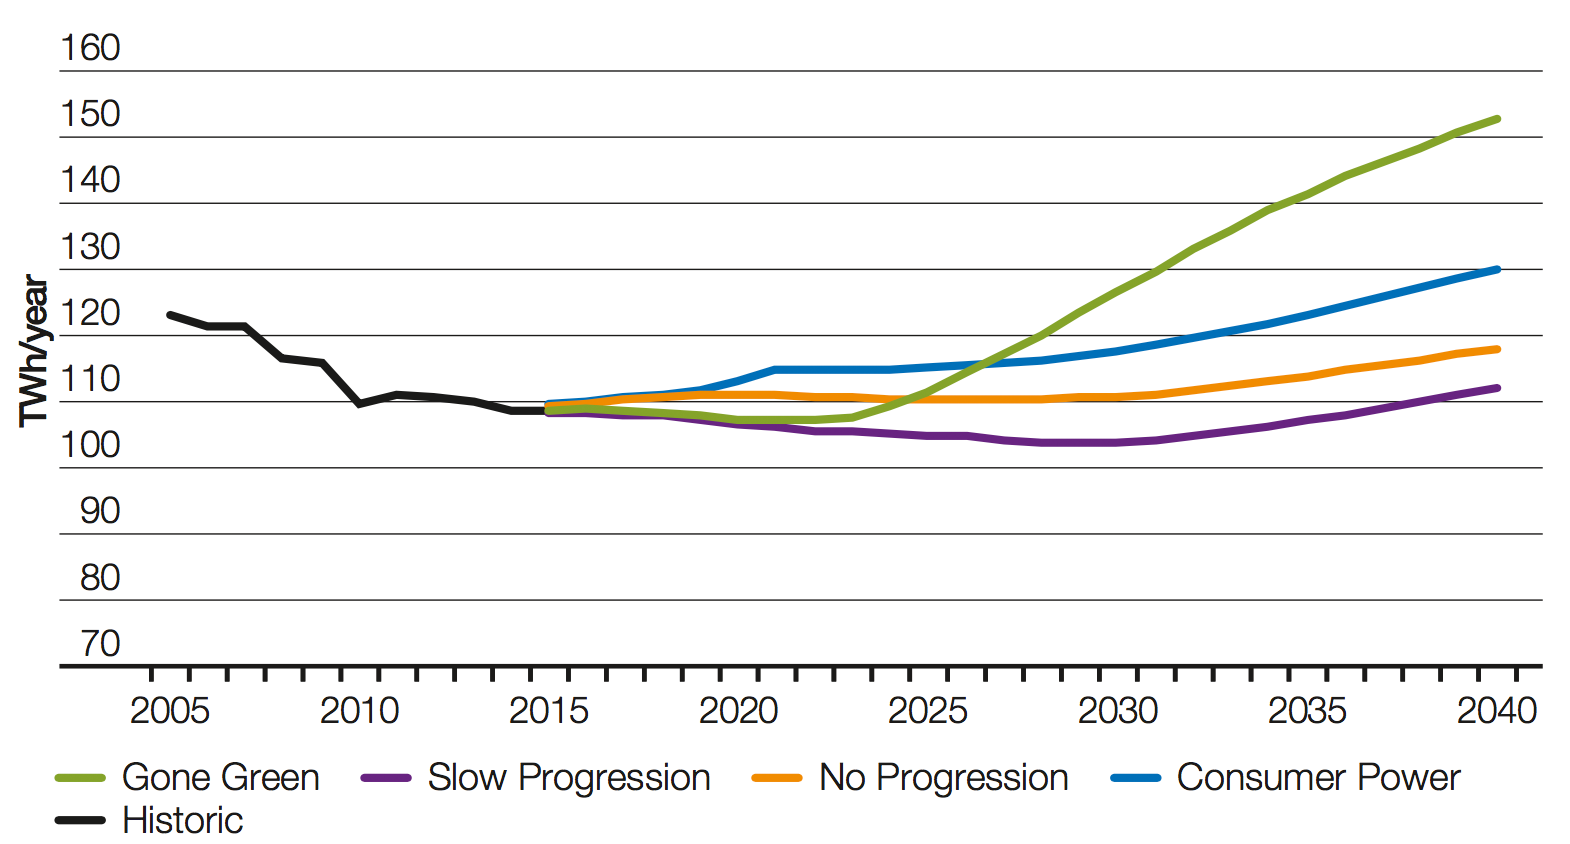
\includegraphics{_introduction/fig/electricity-demand-forecast}
	\caption{Annual residential demand for electricity from FES2016 \cite{FES2016}}
	\label{ch-introduction:fig:electricity-demand-forecast}
\end{figure}

Figure \ref{ch-introduction:fig:electricity-demand-forecast} shows the predicted increase in demand for electric energy when following the UK's 2020 and 2050 goals in reducing green-house emissions.
According to this projection, the annual energy demand will increase by more than 40TWh by the year 2040, if the ``Gone Green'' approach is implemented.
This trend is expected despite increasing device efficiencies, since the shift from oil and gas to electricity, i.e. the electrification, offset these gains.

\begin{figure}\centering
	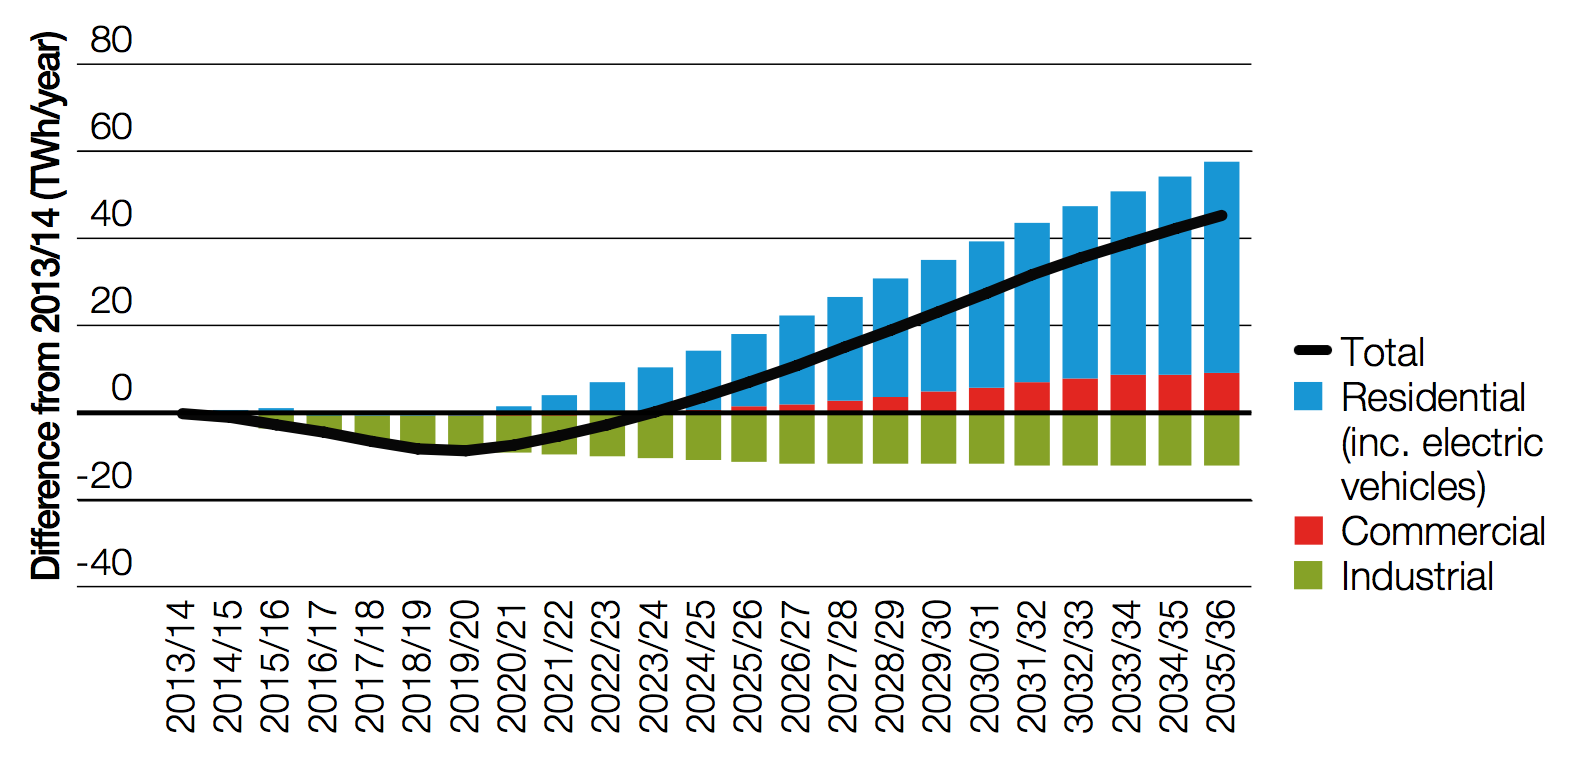
\includegraphics{_introduction/fig/electricity-demand-change-forecast}
	\caption{``Gone Green'' power demand comparison to 2013/14 by type (excluding losses) from FES2015 \cite{FES2015}}
	\label{ch-introduction:fig:electricity-demand-change-forecast}
\end{figure}

\nomenclature[G]{CREST}{Centre for Renewable Energy Systems Technology}

When breaking down the change in demand for electricity, as done in Figure \ref{ch-introduction:fig:electricity-demand-change-forecast}, one can observe how industry sectors are expected to decrease their energy consumption.
Yet residential and commercial sectors are expected to increase their demand and outweigh the industry's energy savings.
Their negative impact on the distribution network is only amplified, since loads in the residential and commercial sectors are typically situated at the network edge, i.e. in the LV distribution network.
This part of the network is its weakest part, since its assets were designed to caters for small powers between 315kVA to 500kVA \cite{EDS08-0115}.
A study based on the findings from \textit{Electricity North West} in \cite{ElectricityNorthWestLtd2014} emphasises the issues that result from residential increase in demand for electricity, of e.g. voltage deviation due to an uptake of LCTs.
The voltage deviation and corresponding power profiles are shown in Figure \ref{ch-introduction:fig:lct-impact}, which was produced by simulating several loads on the IEEE LV Test Case power distribution feeder.
Loads were modelled at high resolution, using the \textit{Centre for Renewable Energy Systems Technology} (CREST) dwelling model \cite{Richardson2010a} and a subset of loads was adjusted using a normal and Rayleigh distribution for solar irradiance and home-charging EVs, respectively.
The findings in Figure \ref{ch-introduction:fig:lct-impact} show how uncontrolled home-charging of EVs significantly reduces voltages in the network, and although solar injection does lead to voltage rises along the feeder, unbalanced injection increases voltage deviation even further.

\begin{figure}\centering
	\subfloat[]{
		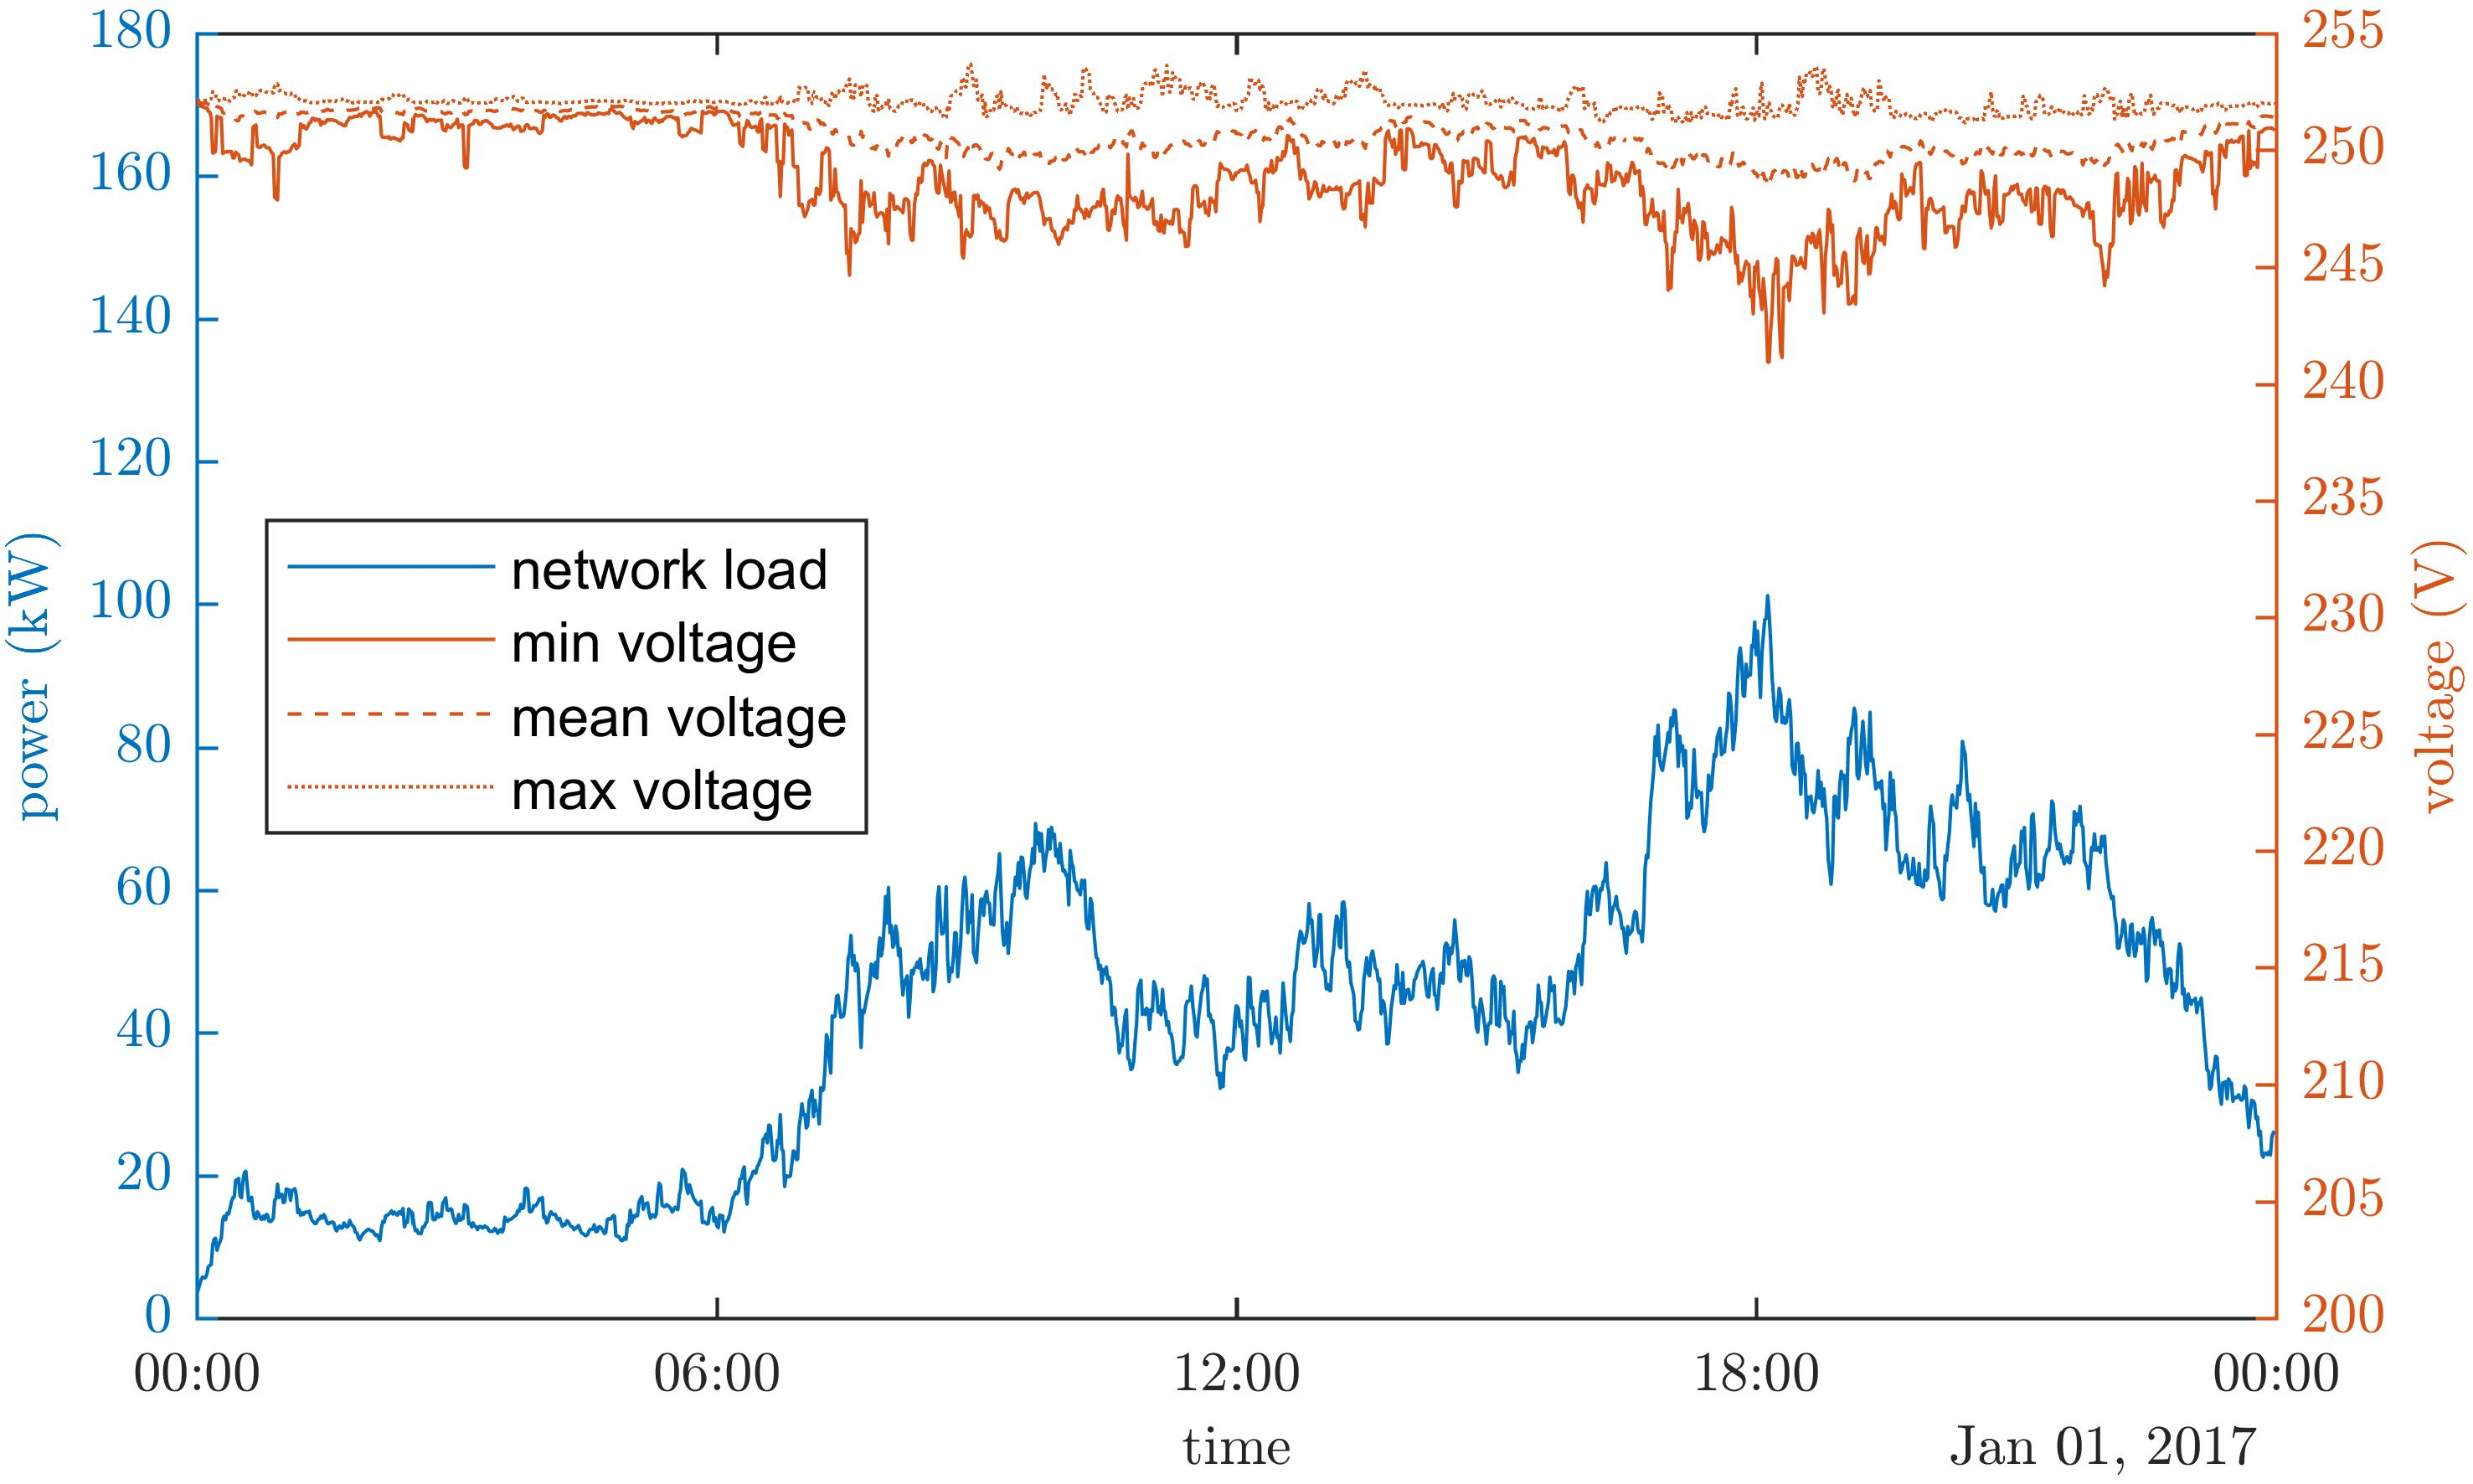
\includegraphics{_introduction/fig/lct-impact-without}
		\label{ch-introduction:subfig:lct-impact-without}
	}
	\vspace{1mm}
	\subfloat[]{
		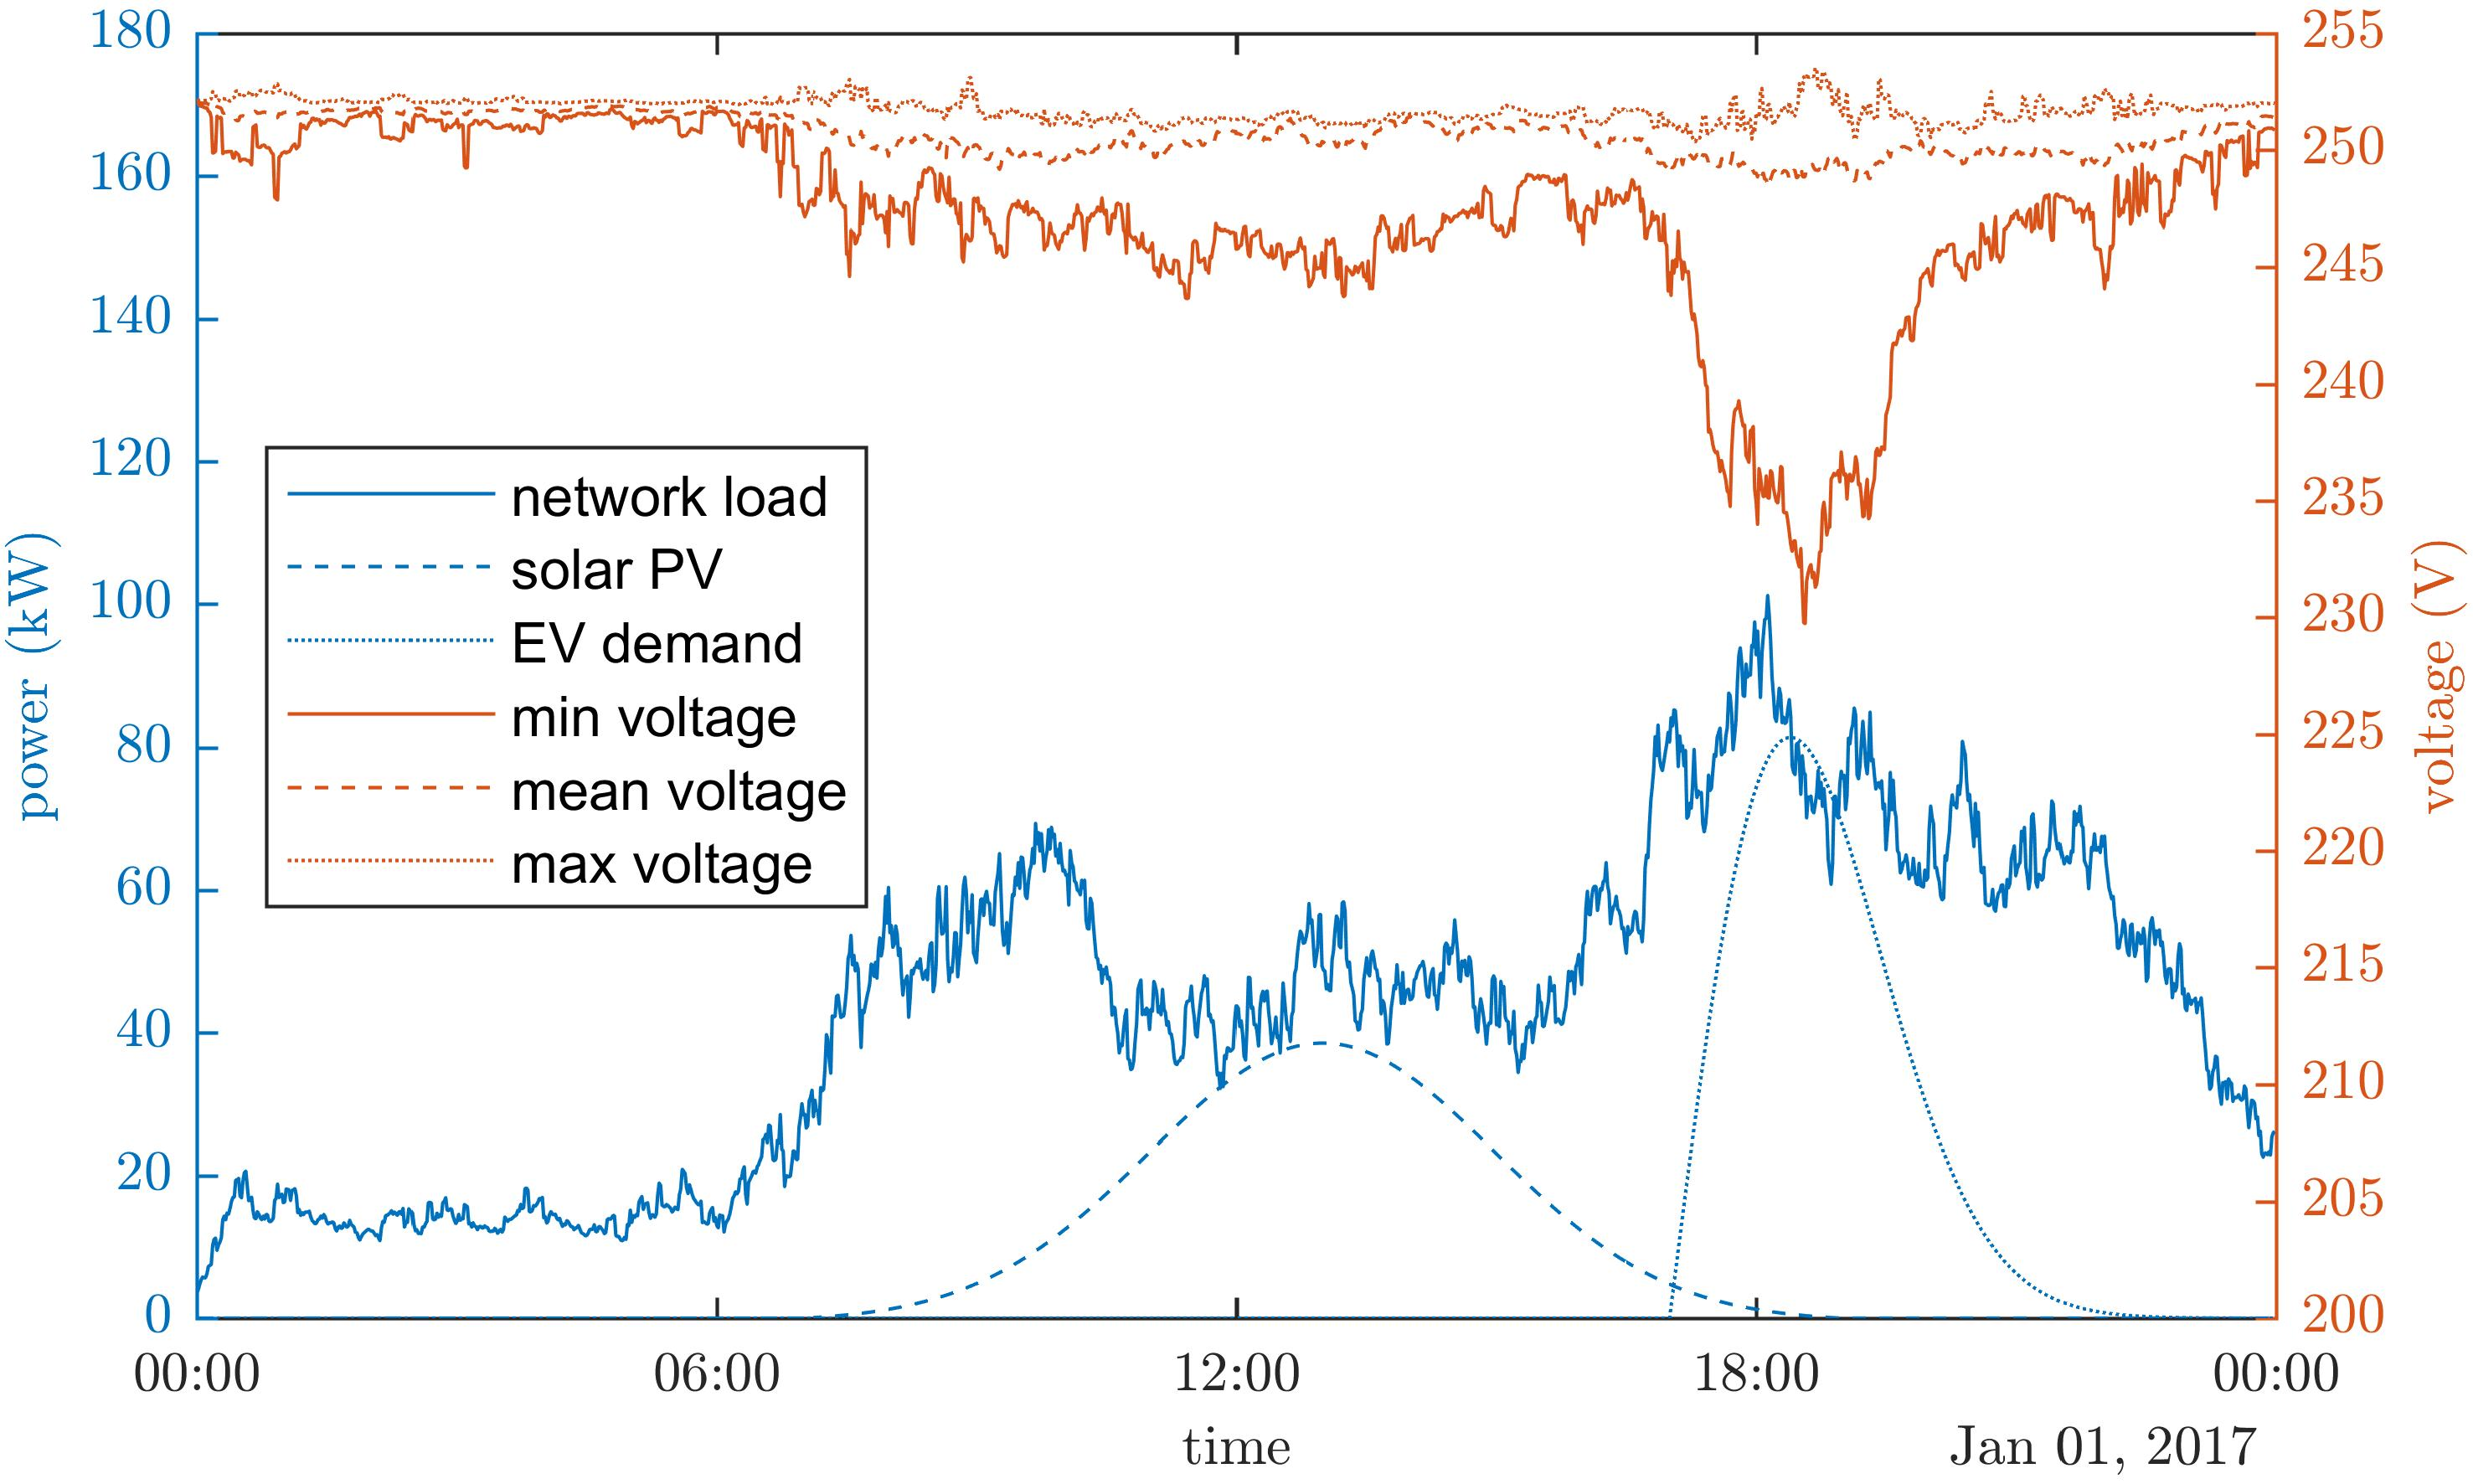
\includegraphics{_introduction/fig/lct-impact-with}
		\label{ch-introduction:subfig:lct-impact-with}
	}
	\caption{Study that compares impact on network voltages due to an uptake in LTCs on the IEEE LV test case: (a) does not contain any PV generation or EV loads; in (b) 20\% of all customers have PV generation with a peak generation of 3.5kW \cite{MongooseEnergy2015} and 20\% of all customers own EVs with Mode-2 home-charging capabilities at 7.4kW \cite{SustainableEnergyAuthorityofIreland2015}.}
	\label{ch-introduction:fig:lct-impact}
\end{figure}

Such a voltage drop behaviour was achieved with a relatively low rate of LCT adaptation in the residential environment, therefore strict regulation is in place to assure continuous operation without violating any operating constraints.
Otherwise additional voltage deviation, unbalanced network operation or potential asset overloads could be the result.

Traditional network planning approaches to follow these regulation were used to circumvent constraint violations.
These approaches follow the commonly used practice of aggregating a large number of customers and designing the power delivery network to cater for their largest probable demand, i.e. the After Diversity Maximum Demand (ADMD) method \cite{Richardson2010a}.
This ADMD method has remained the same for many years and uses historical load analysis and standard growth assumptions that are both no longer valid in this unprecedented LCT uptake scenario \cite{Yunusov2016}.
To make things worse, LV networks in the UK are generally unmonitored once installed.
Distribution Network Operators (DNOs) have become aware of this issue and are developing updated planning strategies involving ``smart'' and ``flexible'' electricity grids \cite{Fang2012}.
However, in situ equipment that will become subject to the same adaptation of LCT needs to be managed actively via innovation in the use of existing and new technologies; otherwise both frequency of service disruptions and customer minutes lost will increase alongside the proliferation of LCTs \cite{Ault2008a}.

\subsection{Solutions to mitigate impact of LCT}
\label{ch-introduction:subsec:solutions-to-mitigate-impact-of-lct}

Two solutions exist, allowing DNOs to support LV network's operation: 
\begin{enumerate*}
	\item reinforcement of in situ network assets;
	\item deployment of network support equipment.
\end{enumerate*}
Whilst network reinforcement would certainly address immediate issues of current network capacity constraints, this approach is also the more expensive and disruptive option.
More specifically, customer will need to deal with outages during periods of asset upgrades (e.g. transformer upgrade and line re-conductoring after secondary transformers' tap settings have been adjusted).
Therefore, alternatives to defer or avoid network reinforcements have been sought and assessed \cite{Harrison2007, Zangs2016a, VanderKlauw2016d, Greenwood2017}.
Most promising alternatives are to install flexible and controllable Distributed Energy Resources (DERs), or more specifically: Battery Energy Storage Solutions (BESS) \cite{Wade2010}.
BESS has not only seen significant advancements in technology, but also received increasing attention in both academic studies and industry trials \cite{Palizban2016}.

Installing BESS on a strategic location in the LV network brings several advantages to DNOs' control over the network's performance.
Roles for BESS are addressed in the subsequent section, i.e. Section \ref{ch-introduction:subsec:role-of-energy-storage-a-survey}.
However, a few examples of potential benefits from BESS include the regulation of voltages to stay within statutory operating bands \cite{Yang2014}, shaving peak loads to relieve stress from the installed network assets \cite{Bennett2015}, and reducing phase unbalance to increase network efficiency \cite{Wang2015b} .
Whilst the questions regarding locating and scaling of BESS have mostly been addressed, BESS control can be split into two complementing yet unmarried approaches:

\begin{enumerate}
	\item ``off-line'' control, using load forecasts and BESS schedules, and
	\item ``on-line'' control, using Set-Points Control (SPC), Model Predictive Control (MPC) or similar dynamic control methods.
\end{enumerate}

Furthermore, with the anticipated uptake of household BESS, mechanisms to control several storage systems also need to be considered.
For instance, several industry leaders propose to store solar energy in order to support charging of EVs \cite{Baumann2017}.
Without rooftop PV installations, batteries need work in a cooperative manner to not impose additional strain onto the network.
The full review of storage control strategies to achieve both off-line and on-line, as well as centralised/individual and distributed battery control is presented in Section \ref{ch-literature:sec:control-of-energy-storage}.

\subsection{Role of energy storage - a survey}
\label{ch-introduction:subsec:role-of-energy-storage-a-survey}


\begin{figure}\centering
	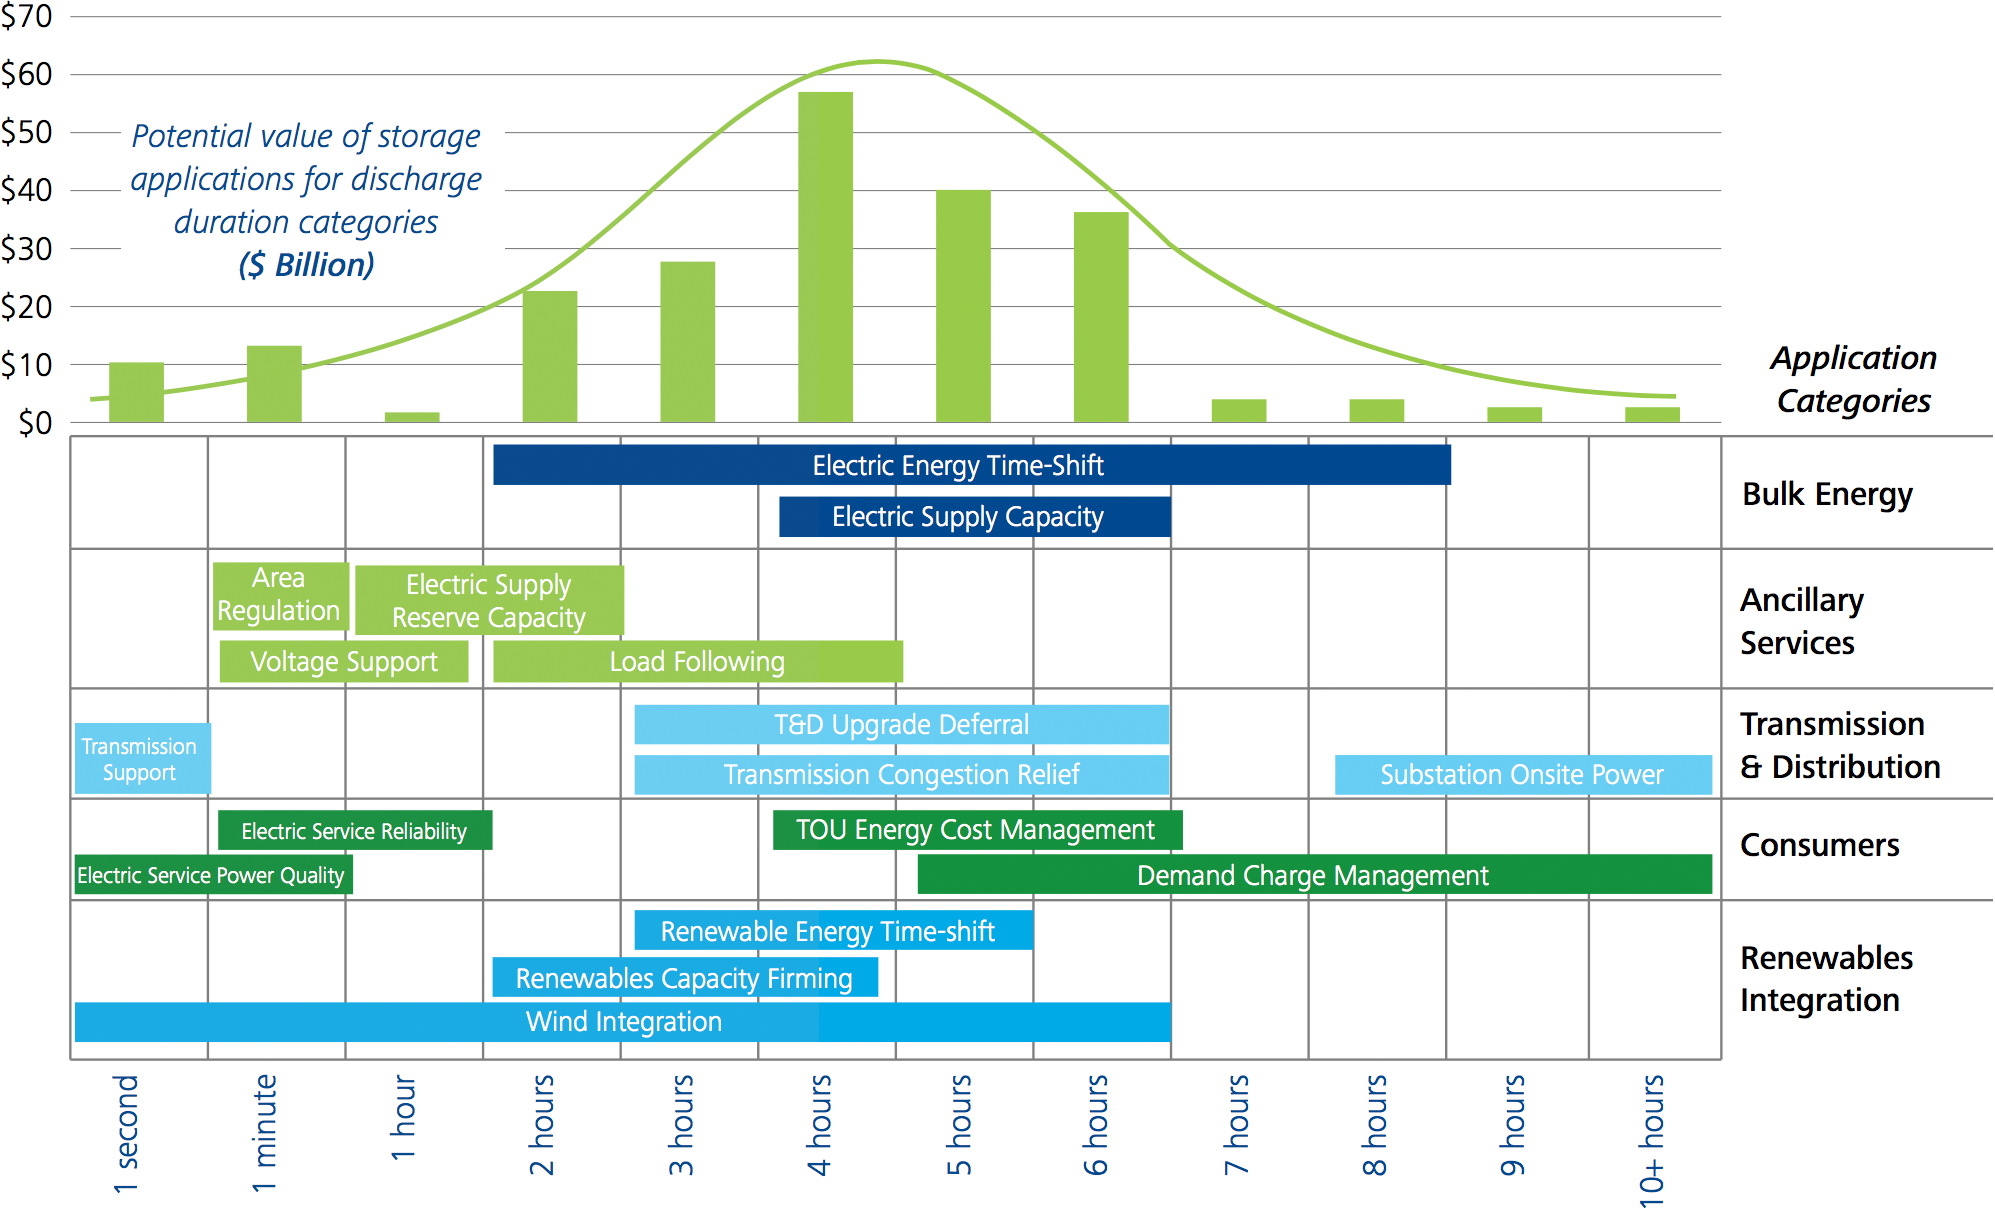
\includegraphics[width=\textwidth]{_introduction/fig/storage-financial-benefits}
	\caption{Energy storage applications and corresponding value for various discharge durations \cite{Deloitte2016}}
	\label{ch-introduction:fig:storage-financial-benefits}
\end{figure}

The idea of using energy storage in the electricity grid has been discussed for quite some time, and its important role in future energy systems has already been identified in the 70s \cite{Kalhammer1979}.
As the name suggests, electrical energy storage systems have the ability to both consume, store, and release electrical energy by converting it into a different form of energy.
Depending on the rate at which energy can be consumed and released, i.e. the system's power, as well as the amount of energy that can be stored, i.e. system's capacity, different functions can be provided.
A study for the Department Of Energy (DOE) showed that, when correctly exploited, these functions can yield direct financial benefits of \$157.56 billion over an estimated 10 year system lifecycle \cite{Eyer2010a}.
Figure \ref{ch-introduction:fig:storage-financial-benefits} shows these benefits in relation to their typical discharge period, and links them to their associated functions, too.
Here, Time Of Use (TOU) energy cost management yields the largest economic profit, yet from a historical point of view, bulk energy storage has played the most important role in the energy system.

Nowadays, storage can also tap into emerging revenue streams and perform additional functions.
As identified in several review articles \cite{Chen2009, Katsanevakis2017, Guney2017}, the key roles and applications of energy storage systems, regardless of profitability in the current market situation, can be identified as follows:

\textbf{Energy shifting - arbitrage}: This function uses the difference in energy price to yield revenue.
More specifically, as energy pricing is expected to become more dynamic and responsive to current energy demand and generation, storage is controlled to charge when energy prices are low and discharge when energy prices are high \cite{Chen2009, Leou2012}.
Such dynamic pricing schemes are expected to emerge due to significant changes in demand at morning and evening peaks \cite{Koohi-Kamali2013}.

\textbf{Supply capacity}: In order to meet future energy demand, energy suppliers commit their resources in advance.
Doing so allows them to plan for their operation and solve the economic dispatch problem.
With increasing demand, the supply volume will have to increase, too.
However, it is predicted that energy storage can defer or even avoid investments in power plants, assuming they are sized accrodingly (i.e. several 100MW)\cite{Dobie1998}.
Bulk energy storage was the first choice to support supply capacity.
One example is pumped hydro-electric energy storage, which has seen a global growth of 127GW since 1979 \cite{Rehman2015, Barbour2015, Barbour2016}.

\textbf{Ancillary services}: These services are of interest to transmission and distribution system operators since they support the operation of their networks.
For example, load following and frequency regulation are two complementing applications of that address the imbalance between demand and supply \cite{Bevrani2011}.
In case of a severe imbalance that resulted in network outage, black start is also a function that can be supplied by energy storage \cite{Cole1995, Kashem2007}.
Since modern energy storage systems can absorb and inject both active and reactive power, they can also provide voltage support \cite{Kulkarni2005}.

\textbf{Grid stability}: To make the grid more resilient to network faults (e.g. short-circuit or loss of a large generator), or to overcome scheduled network outages, energy storage can be used as an intermittent energy source \cite{Kundur1993}.
To provide optimal operation conditions for energy generators, storage can support rotor angle stability and voltage stability by injecting active and reactive power at the point of common coupling \cite{Chakraborty2012, Kolluri2002}.
Furthermore, sub-synchronous resonance and harmonic interference can also be reduced \cite{Wang1994}.
This coupling resonance can occur between electrical and mechanical systems and can damage the mechanical structure due to repetitive stresses and strains.

\textbf{Upgrade deferral}: As already stated in Section \ref{ch-introduction:subsec:solutions-to-mitigate-impact-of-lct}, both transmission and distribution systems would have to be upgraded unless energy storage could provide network-support functions.
By deferring network upgrades, network assets will be used more efficiently, and customer disruptions will be avoided \cite{Sayer2007, Eyer2010a}.
Furthermore, in areas where the expected load has already been met and growth has levelled out, deployed energy storage is flexible enough to provide alternative functions (unlike other network assets) \cite{Huff2013}.

\textbf{Transmission charges}: In scenarios where generators are charged to use transmission systems (due to the capacity limitations of the transmission system), energy storage could take advantage of the price structure to maximise the profit from the generated energy \cite{Sayer2007, Leou2012}.

\textbf{Congestion relief}: High congestion at substations of heavily loaded transmission or distribution lines can be tackled by co-located energy storage units \cite{Saez-de-Ibarra2013a, Kulkarni2005}.
This can be achieved by e.g. shaving peak load or relaxing the energy requirements from distributed generation \cite{Reihani2016, Gerards2016d}.

\textbf{Service reliability}: In areas where a string grid connection is required to assure e.g. industry operations, an ``uninterruptible power supply'' may be required.
Traditionally, these power supplies were diesel backup generators, but modern energy storage technology can provide similar services at lower cost \cite{Schoenung2001} (particularly when including alternative revenue streams).

\textbf{Power quality}: Sub-cycle and harmonic distortions on can severely deteriorate power quality, since they can have unwanted effects on connected equipment (similar to the issue of sub-synchronous resonance at the generation side).
Energy storage with modern power electronics could be capable of providing power filtering functions that suppress those distortion \cite{Putrus2007}.
This feature could be of particular interest to LV networks in the UK, since customers are arbitrarily connected to a single phase of a three-phase network.
Therefore, the discrepancy of power quality between the phases is even larger, yet available energy storage resources could even address this issue \cite{Miret2009} (especially when considering household connected units).


\textbf{Time-of-use energy charges}: A hurdle to DSM through flexible tariffs or TOU tariffs is the reason that consumers would have to adjust their energy consumption based on external price signals, which many are do not want to do.
Energy storage could however decouple the consumer form these tariffs and allow them to continue with their normal lifestyle \cite{Khani2014}.
Additionally, when exploiting the energy price difference, storage could even supply arbitrage functions to some customers and reduce their electricity bill \cite{Nair2010a}.
For customers with local generation, e.g. PV installation, their bill can be reduction even further.
This would be done by storing the generated energy until a period of high energy prices arises.
At this time energy storage could release the energy to maximise self-consumption \cite{Luthander2016}.

\textbf{Demand charges}: Larger customers, i.e. industrial and commercial loads, are not only charged for their total energy demand, but also their for their largest continuous power demand \cite{Oudalov2007, Mackey2013}.
Therefore, a factory that may use a relatively small amount of energy over a comparatively short amount of time, is billed accordingly.
After all, the infrastructure to deliver the required power needs to be installed and maintained.
In this scenario, energy storage could reduce the intermittent power demand without significantly increasing the total energy demand, and therefore reduce demand charges for larger customers \cite{Aghaei2013}.

\textbf{Renewables integration}: Unlike traditional energy sources, renewables have are highly volatile and have limited availability.
Since their availability, i.e. for solar PV, may not align with periods of high demand, i.e. during morning and evening, arbitrage functions may be provided to maximise the use of renewable generation - i.e. renewables ``shifting'' \cite{Zakeri2015}.
Furthermore, by discharging energy storage during times of low renewable generation, e.g. due to cloud cover or varying wind \cite{Jewell1987}, a continuous supply of energy can be assured - i.e. renewables ``smoothing''.
And lastly, if a renewable resource was committed for longer periods of time, yet the associated energy forecasts overestimated its generation capacity, storage can supply the gap to avoid balancing charges - i.e. renewables ``firming'' \cite{Chakraborty2012}.

\subsection{Smart control}
\label{ch-introduction:subsec:smart-control}

\hl{WRITE THIS}

\subsection{Challenges to control BESS}
\label{ch-introduction:subsec:motivation}

From the extensive catalogue of possible roles for energy storage in the electricity grid that was presented in Section \ref{ch-introduction:subsec:role-of-energy-storage-a-survey}, the focus of the research in this thesis is put on aiding DNOs to manage and operate their power distribution networks.
More specifically, battery energy storage is the main focus since is has the potential to defer or even mitigate costly network reinforcements.
Modern battery technology allows the storage of electrical energy in ever-decreasing form factory, whilst power electronics technology becomes more efficient at integrating batteries into power networks.

As shown in the literature review in Chapter \ref{ch-literature}, methods of controlling BESS to optimise power flow have been of great research interest.
However, the impact on particular key parameters of the three-phase networks still need to be investigated.
Subsequently, the challenge of applying real-time corrections to BESS schedules in order to decrease peak demand whilst obeying to technical and operational constraints is also a remaining research question.
Also, since the expected uptake of distributed BESS through proliferation of household storage solutions (e.g. to counteract the impact of EVs) requires sophisticated coordination mechanisms, two additional research challenges have been identified.
The first challenge focuses on improving cooperating device behaviour despite communication disturbances (i.e. through message desynchronisation), and the second builds upon the findings from key network improvements to construct a functioning BESS control mechanism despite the absence of a telecommunications infrastructure.







\section{Motivation}
\label{ch-introduction:sec:motivation}



\section{Problem statement and research objectives}
\label{ch-introduction:sec:problem-statement}

The focus of the research presented in this thesis is put on aiding DNOs to manage and operate their power distribution networks by installing energy storage into their distribution networks in order to counteract the effects from electrification of heat and transport sectors as well as the decarbonisation of the grid itself.
Therefore BESS control is the main focus of this work since BESS is a rapidly improving technology that has the potential to defer or even mitigate costly network reinforcements.
Modern battery technology allows the storage of electrical energy in ever-decreasing form factors, whilst power electronics technology becomes more efficient at integrating batteries into power networks.
As shown in the literature review in Chapter~\ref{ch-literature}, methods to control BESS, for instance, in order to optimise power flow, have been and still are of great research interest.

Therefore, the aim of this thesis is to present a contribution in BESS control to improve grid operation and reliance, when deploying it in the UK LV distribution network.
Given the already established control approaches of ``off-line'' and ``on-line'' control, merging the two in order to take advantage of BESS schedules and real-time information is still an open research challenge.
Subsequently, applying real-time corrections to BESS schedules in order to decrease peak demand whilst obeying to technical and operational constraints is also an identified research challenge.
Since the expected uptake of distributed LCTs and DERs through proliferation of household-connected storage solutions (for example to support PV integration or to counteract EV impacts) requires ``smart'' coordination mechanisms.
When requiring communication to implement this smart coordination, another challenge exists in developing algorithms that function despite communication disturbances (i.e. through message desynchronisation).
Lastly, in the case where communication-less coordination of distributed devices is sought, the challenge of assuring equal device usage whilst providing network support (for example to guarantee a minimum lifetime) has also been identified.

These research challenges are extensively reviewed in the literature review in Chapter \ref{ch-literature}, and in accordance to these identified key challenges that motivate the conducted research, a set of objectives is presented in order to achieve the aim of contributing to the existing field:

\begin{enumerate}[
labelindent=*,
style=multiline,
leftmargin=*,
label=\textbf{Objective~\arabic*}
]
	\item \label{objective-1} Develop a control mechanism for a single BESS to further improve three-phase network operation without \hl{changing half-hourly real power schedules by adjusting BESS power phasors and reactive power injection}.
	\item \label{objective-2} Develop a control mechanism that \hl{dynamically adjusts half-hourly schedules on a sub-half-hourly basis, hence modifying the half-hourly schedule to reduce daily load peaks by combining control elements from both off-line and on-line control}.
	\item \label{objective-3} Develop and compare operation of a scheduling algorithm that manages the charging behaviour of multiple BESS by submitting it to performance analysis in a synchronised and desynchronised communication environment.
	\item \label{objective-4} Develop a communication less control strategy for distributed BESS by \hl{modifying the traditional and robust Additive Increase Multiplicative Decrease (AIMD) algorithm by introducing a threshold dependent scaling of the additive term} and by individually assigning control parameters.
\end{enumerate}



\section{Contributions to knowledge}
\label{ch-introduction:sec:contributions}

The literature that is reviewed in Chapter~\ref{ch-literature} introduces the key contributions surrounding the control of energy storage in power distribution networks, and therefore supports the thesis problem statement in Section~\ref{ch-introduction:sec:problem-statement}.
This review concludes by identifying gaps in literature which are used as starting points to formulate the research objectives and resulting research contributions.
These contributions are summarised as follows:

\begin{itemize}
	\item
	An iterative closed-loop power adjustment method is presented, which controls a DNO owned storage devices in such a way that its three-phase power flow improves LV network operation.
	This contribution is the result of \ref{objective-1} and is achieved by using the device's flexibility in assigning active power to the three phases, and by using the remaining capacity of power electronics to inject or absorb reactive power, whilst obeying to an underlying half-hourly BESS schedule.
	\item
	A dynamic control method to merge off-line BESS scheduled control with an on-line power prediction mechanism (i.e. Model Predictive Control) is developed to minimises both the imminent sub-half-hourly load peaks as well as the day-ahead half-hourly load peaks.
	This contribution is the result of \ref{objective-2} and is achieved by merging schedules that are based on real load forecasts with an autoregressive model that is fed by real load data.
	\item
	A robust charge scheduling algorithm for multiple, distributed entities is developed to prevent charging spikes from adding excessive stress onto the distribution network which would otherwise experience capacity shortages.
	This contribution is the result of \ref{objective-3} and is achieved by implementing a ``Multi-Agent System'' (discussed in the literature review in Section~\ref{ch-literature:subsec:centralised-and-distributed-control}) on a compute cluster to compare algorithm performance for both synchronised and desynchronised message exchange.
	\item
	A communication-less distributed control method is developed that improves the traditional Additive-Increase Multiplicative-Decrease (AIMD) algorithm to achieve cooperative behaviour of multiple BESSs in order to mitigate the impact of co-located ``dumb-charging'' EVs.
	This contribution is the result of \ref{objective-4} and is achieved by individually assigning control parameters to all BESS whilst using local voltage measurements to infer the current network status.
\end{itemize}


\section{Thesis structure}
\label{ch-introduction:sec:thesis-structure}

The structure of this thesis is organised as follows:

\begin{itemize}
	\item
	\textbf{Chapter~\ref{ch-literature}} carries out an extensive review of the literature surrounding the field in order to support the problem statement and proposed contribution.
	\item
	\textbf{Chapter~\ref{ch1}} develops a BESS scheduling mechanism and identifies key network parameters that are used in their corresponding cost functions to improve network operation.
	Then, this chapter address \ref{objective-1} by presenting a method that assigns a BESS schedule to the three-phase power distribution network whilst minimising the aforementioned cost functions; therefore improving network operation.
	Results are compared against a ``baseline'' and a ``normal'' (or traditional) operation case by assessing them on a temporal and probabilistic level.
	\item
	\textbf{Chapter~\ref{ch2}} then extends the work in Chapter~\ref{ch1} by presenting a dynamic control method that adjusts a half-hourly BESS schedule at sub-half-hourly temporal resolution in order to reduce both volatile and the daily load peak.
	This is achieved by combining two PID compensated control loops with a MPC and BESS schedule.
	Therefore, this chapter addresses \ref{objective-2}.
	\item
	\textbf{Chapter~\ref{ch3}} addresses \ref{objective-3} by presenting a cooperative battery charging algorithm that is deployed on a Multi-Agent System and assessed in both a synchronised and desynchronised communication environment.
	In this chapter, both algorithm convergence and algorithm performance is compared between its implementation in the synchronised and desynchronised scenario.
	\item
	\textbf{Chapter~\ref{ch4}} develops a stochastic EV demand model that is based on real vehicle mobility data, and it will develop a control algorithm for distributed BESS to mitigate the negative impact from the resulting EV demand.
	This chapter address \ref{objective-4}, the final research objective, by extending the Additive-Increase Multiplicative-Decrease algorithm to enable cooperating BESS operation under the absence of a shared communication infrastructure.
	\item
	\textbf{Chapter~\ref{ch-conclusions}} presents a detailed conclusion that relates all findings back to the initial problem statement and the overarching aim of the presented PhD thesis.
	Also, this chapter highlights potential future work based on the findings from the conducted research.
\end{itemize}
\chapter{Literature Review of Storage Control}
\label{ch-review}

\section{Overview}
\label{ch-literature:sec:overview}

With the ongoing electrification and decarbonisation of the heat and transport sector, demand across the electricity network is expected to double by 2050 \cite{Wilks2010}.
One contributor towards this increasing demand is the expected uptake of LCTs as they start to penetrate power distribution networks.
Also, this uptake of LCTs is expected to not progress evenly throughout the network; instead clusters of early adopters are predicted to form \cite{Poghosyan2014}.
Such a scenario will result in LV networks to exceed their operational constraints even whilst the rate of LCT adaptation is at a relatively low national rate \cite{Poghosyan2014}.
Conventional reinforcement to extend the network's capacity is effective but expensive.
Together with recent availability of load information, due to the distribution and installation of smart-meters, the opportunity arises for DNOs to develop energy storage control strategies in order to achieve the greatest performance and add most benefits to their distribution networks.

In fact, according to the Department of Energy's global energy storage database, there are more than 1200 energy storage projects worldwide.
In the UK, as of 2016, 27 of those are installed and accumulate to an energy storage capacity of 33GWh \cite{Garton2016}.
Out of all global energy storage projects, 61\% use ``electro-chemical energy storage technology'', i.e. rechargeable batteries, and 49\% of those Battery Energy Storage Systems (BESS) are rated at less than 250kW.
Their sizes and ratings make such BESS suitable for deployment in distribution networks, and the figures in the energy storage database indicate that 131 of these projects are indeed used for LV network support \cite{DOE-GESD}.

A general survey of different roles for energy storage have already been presented in Section \ref{ch-introduction:subsec:role-of-energy-storage-a-survey}.
However, to align with the focus of this thesis on improving UK power distribution networks, Chapter \ref{ch-literature} will provide an extensive review on BESS applications and projects that support LV network operation; i.e. projects concerning voltage control mechanisms and power flow management.
The structure of this chapter is as follows.
First, in Section \ref{ch-literature:sec:topology-of-lv-network}, an overview of the UK power distribution network is given.
Then, the literature regarding energy storage projects and their applications in LV networks is reviewed in Section \ref{ch-literature:sec:energy-storage}.
Afterwards, in Section \ref{ch-literature:sec:control-of-energy-storage}, diffrent control approaches for energy storage are reviewed and compared.
In the end, in Section \ref{ch-literature:sec:literature-gaps}, the gaps are identified to highlight the research contribution and support the problem statement of this thesis.


\section{Background}
\label{ch-review:sec:background}

\subsection{Entity Management in Power Networks}

\subsection{Device Control Paradigms}

\subsubsection{Idealised Control for Control Theory}

\subsubsection{Realistic Control for Application Driven Research}

\section{Related Work}
\label{ch-review:sec:related-work}

\subsection{Storage Projects}

\subsection{Multi-Agent System Based Control}

\subsubsection{Centralised Architecture}

\subsubsection{Decentralised Architecture}


%% Discuss types of energy storage and how they are proposed to be used
%
%% Types: Hydro, compressed air, flywheel, battery etc
%% Application: Grid support (peak shaving), DG uptake (flexibility), economic (arbitrage & market)
%
%Large scale energy storage solutions like pumped storage hydro-electric have been in used for a long time to provide load levelling and energy reserve functions. In 1982, Wicks et.al. \cite{Wicks1982} proposed a linear programming approach to automatically control such an energy storage solution. This first step was 
%
%The idea of using batteries to support network operation is not new. In 1982, DelMonaco et.al.\cite{DelMonaco1982} highlighted the basic considerations when planning the operation and maintenance of grid connected batteries. They were amongst the first to publicly identify the role of energy storage beside distributed renewable generation, and the associated issues of bidirectional power flow and islanding of isolated branches. 
%
%Storage is great when combined with DER
%\cite{Papathanassiou2006}
%

\section{Energy Storage Control Methodologies}
\label{ch-review:sec:energy-storage-control-methodologies}

Two main control approaches \cite{Hida2010}: plan based and responsive.

% Speak about common control methods for network
% SCADA, Microgrid, Forecasting, Scheduling, Peak-Shaving, DSM, etc

\subsection{Set Point Control}

\subsubsection{Principle}

\subsubsection{Requirements}

Centralised i.e. SCADA approach, or distributed i.e. Multi-Agent System.

\subsubsection{Applications}

Autonomous network control \cite{Nogaret1997a}

Traditional set point control \cite{Leadbetter2012}.

Applications cover hybrid fuel cell and battery \cite{Jiang2007}, wind farm \cite{Teleke2009a}.

\subsection{Scheduled Control}

\subsubsection{Principle}

\subsubsection{Requirements}

Forecasting principle \cite{Ramanathan1997}

Review and comparison of 5 forecasting techniques at hourly resolution \cite{Moghram1989}.

Long-term hourly forecast \cite{Filik2011}

Hourly forecast using regression \cite{Papalexopoulos1990}

Peak forecasting \cite{Barakat1990}

Day- or Week-ahead forecast (short term forecast) \cite{Hyde1997}

Forecasting \cite{Charlton2014}

Forecasting \cite{Taieb2013}

Schedule errors due to volatility (MV and LV) \cite{Haben2014}.

\subsubsection{Applications}

Peak reduction scheduling algorithm \cite{Rowe2014a}

\subsection{Hybrid Control}

%\subsubsection{Rule-Based Control}
%
%\subsubsection{Control Based on Artificial Intelligence}


\section{Summary of Gaps in Litearture}
\label{ch-review:sec:summary}

\chapter{Improving network performance by adjusting battery operation at sub-half-hourly resolution}
\label{ch1}

\singlespacing
\epigraph{\textit{M. J. Zangs, et al., ``On-line adjustment of battery schedules for supporting LV distribution network operation,'' 2016 International Energy and Sustainability Conference (IESC), Cologne, Germany, 2016, pp. 1-6.}}{--- Available: http://dx.doi.org/10.1109/IESC.2016.7569485}
\doublespacing


\section{Overview}
\label{ch1:sec:overview}

Due to the trends in energy demand, future network load is expected to increase in both magnitude and volatility.
As a result, DNOs have two choices to address the issues that are expected to result from increased network stress.
They can either invest in network reinforcement or install network support equipment.
For several reasons, e.g. decommissioning cost, installation cost, service disruption, etc., which have been outlined in Chapter~\ref{ch-introduction}, the installation of network support equipment was favoured.
As also mentioned in Chapter~\ref{ch-introduction}, \textit{SSEN} deployed and trialled an Energy Storage Management Unit (ESMU) in some of their Low-Voltage (LV) power distribution networks.
Within the scope of their trials, ESMU had to be controlled to benefit the network, without exceeding or violating any operational constraints.
In order to achieve this kind of operation, ESMU operation had to be scheduled.
During this kind of operation, the system either consumes or injects power, according to a predetermined plan that changes at regular intervals.
For historic reasons and system compliance, this interval was chosen to be of 30 minutes, i.e. at half-hourly period.

Since the ESMU schedule was generated based upon a demand forecast, any resulting impact on the LV network operation is therefore based upon two factors:

\begin{enumerate}
	\item quality of the underlying forecast that is used to generate ESMU schedules, and
	\item network parameters that are used to quantify the improvements that would have been expected, when the half-hourly schedule is applied.
\end{enumerate}

\nomenclature[G]{ERL}{Energy Research Laboratory}
\nomenclature[G]{UoR}{University of Reading}

The previous research that was conducted by the Energy Research Laboratory (ERL) at the University of Reading (UoR) focused on improving half-hourly network operation to e.g. reduce peak load \cite{Rowe2014a, Yunusov2011}.
However, in that research, sub-half-hourly demand variability has not been taken into account.
Therefore, previously used performance parameters, and the corresponding measure of success, did not effectively quantify the ESMU's capability at mitigating negative impacts from this sub-half-hourly demand.

Therefore, this chapter addresses \ref{objective-1} of this thesis (which is outlined in Section~\ref{ch-introduction:sec:problem-statement}), and a closed-loop optimisation method is proposed that adjusts the ESMU's phase powers at a sub-half-hourly resolution in order to improve network operation, whilst maintaining the charging and discharging profile during the corresponding half-hourly period.
Unlike previous work in the field, this approach makes the ESMU follow its  predetermined ESMU schedule, as well as allowing it to respond to high-resolution variations in three-phase network load.

In order to investigate how network operation may be improved, a collection of commonly used parameters are evaluated in a set of corresponding cost functions.
Initially, these cost functions are minimised on an individual basis to inspect their separate impact on network performance.
Then, all cost functions are combined as a weighted sum to form a global cost function, which is used in the final analysis.
For each optimisation approach, power flow simulations are run on a standardised UK power distribution feeder model in the simulation environment OpenDSS.
This chapter therefore addresses the research question, whether sub-half-hourly adjustments to scheduled ESMU operation can significantly improve measured key network parameters.

The obtainment of key network parameters and their corresponding measure of improvement is explained next, in Section~\ref{ch1:sec:key-network-parameters}.
All acquired data and the power network models used for this piece of work are shown in Section~\ref{ch1:sec:data-and-network-models}.
Subsequently, the closed-loop optimisation method is presented in Section~\ref{ch1:sec:closed-loop-optimisation-method}.
At the end of this chapter, all results are presented and discussed in Section~\ref{ch1:sec:results-and-discussion}, and a concluding summary is presented in in Section~\ref{ch1:sec:summary}.


\section{Key Network Parameters and Derived Cost Functions}
\label{ch1:sec:key-network-parameters}

In literature (see Chapter \ref{ch-review}), two distinct approaches have emerged to quantitatively improve the performance of a system:
either cost is reduced or utility is maximised.
Both approaches rely on a mathematical explanation of underlying features that relate to performance of the system.
To recap; utility functions are maximised since they explain how beneficial a system state is, whereas cost should be minimised since they entail a suboptimal system performance.
The choice for this piece of work was to associate key network parameters to tailored cost functions, with the reason that a cost can be minimised to a finite value, i.e. zero.
Utility maximisation on the other hand is a mathematically unbound problem that may reach a maximum, yet this maximum can only be approximated though game theoretic approaches like Pareto- or Nash-Optimality.
In other words, solutions to a cost function where the resulting cost is zero, are by definition optimal solutions, whereas a utility functions can have multiple maxima where optimality classification of these solutions is inherently more difficult.
To illustrate this fact, an arbitrary utility function, $\zeta^{*}(x)$, and an arbitrary (and unrelated) cost function, $\zeta(x)$, have been plotted in Figures \ref{ch1:subfig:sketch-utility} and \ref{ch1:subfig:sketch-cost}, respectively.

\begin{figure}\centering
	\subfloat[Sample utility function]{%
		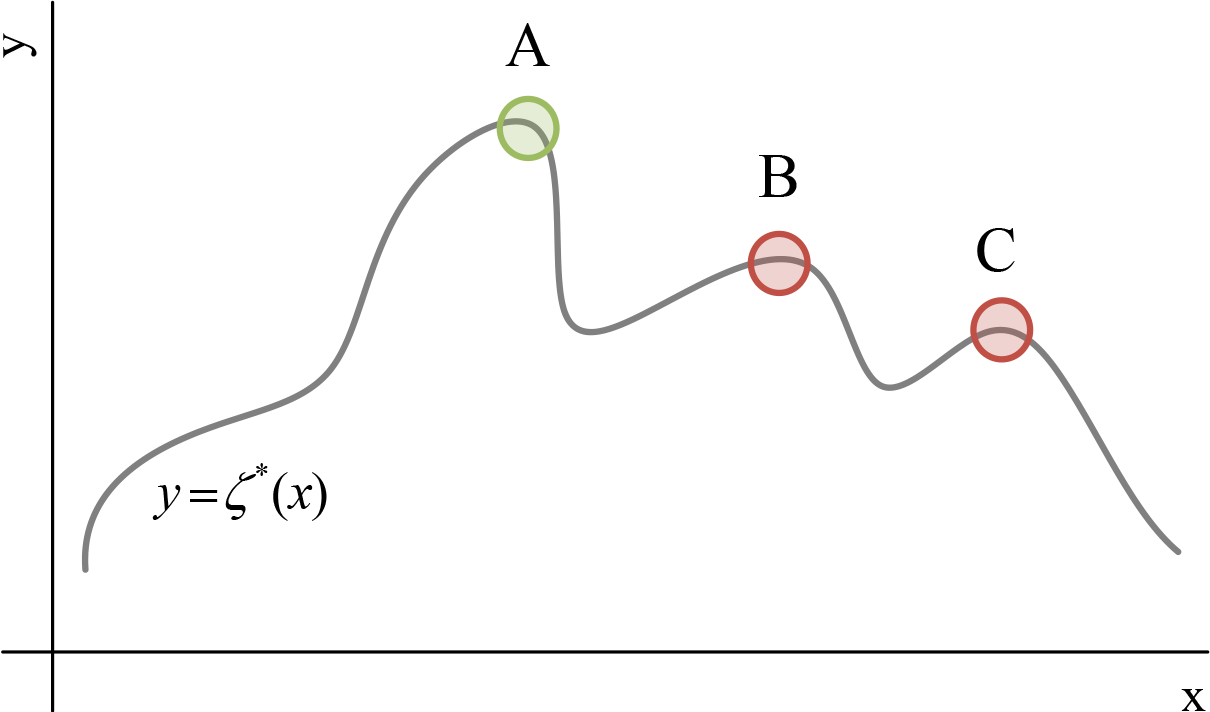
\includegraphics[width=0.45\textwidth]{_chapter1/fig/sketch-utility}%
		\label{ch1:subfig:sketch-utility}%
		}
	\hspace{5mm}
	\subfloat[Sample cost function]{%
		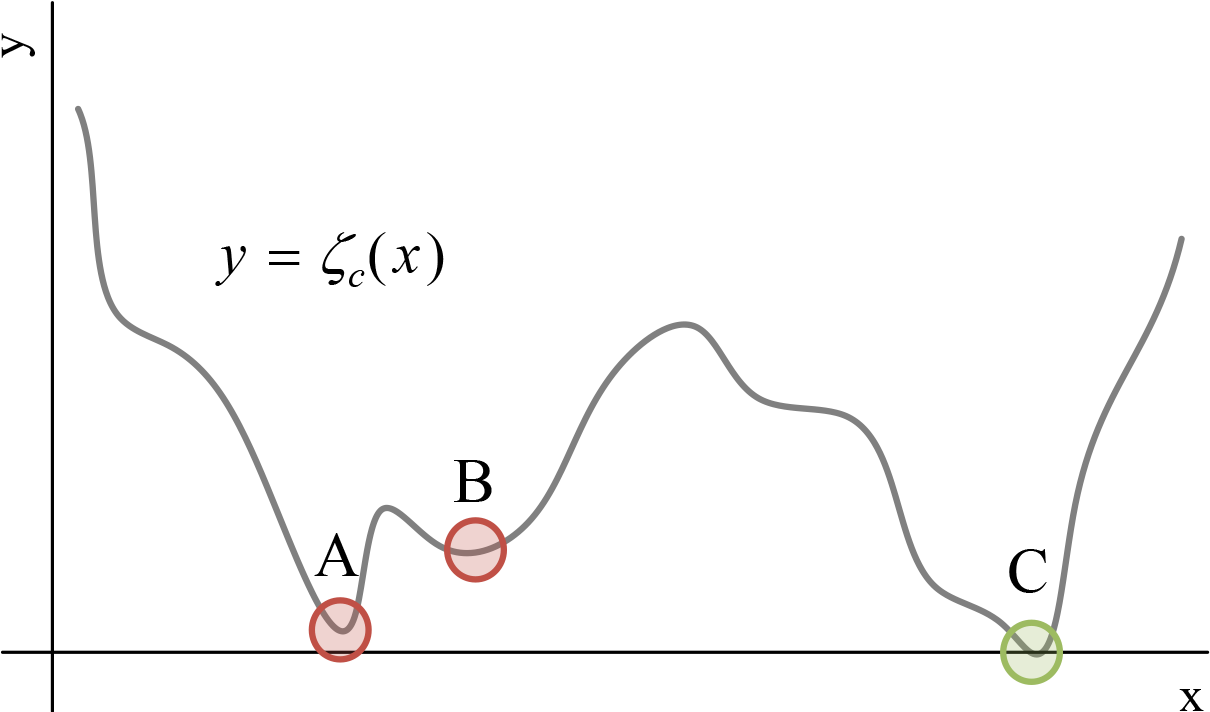
\includegraphics[width=0.45\textwidth]{_chapter1/fig/sketch-cost}%
		\label{ch1:subfig:sketch-cost}%
		}
	\caption{Benefit of using cost function over utility function}
	\label{ch1:fig:sketch-utility-vs-cost}
\end{figure}

These two figures illustrate how the peaks of the utility function are at different, large values of $y$, and the troughs of the cost function tend towards zero.
Both peaks or minima are found using solving algorithms; the most common mathematical solvers are the Gradient Descend Method, Newton-Raphson Method, and Active Set Method.
If the cost or utility function is nonlinear or the system's gradient function can only be approximated more sophisticated algorithms had to be used, e.g. Mixed-Integer Linear Programming, Sequential Quadratic Programming (SQP), Genetic Algorithm, Particle Swarm Optimisation or the Interior Point Method.
Depending on the starting conditions of those solvers, i.e. the initial values for $x$, different maxima or minima (i.e. points $A$, $B$ or $C$) may be found.
In the example above, the best solution for $\zeta^{*}(x)$ is at point $A$, whereas the best solution for $\zeta(x)$ is at point $C$.
Whilst point $A$ represents the highest utility, it is difficult to determine whether this maximum is a most optimal solution since utility is inherently unbounded, i.e. $\zeta^{*}(x) \in (-\infty, \infty) \forall x$.
For the cost function on the other hand, point $C$ is represents an absolute minimum and optimal solution since the cost function's range is bounded to be greater or equal to zero, i.e. $\zeta(x) \geq 0 \forall x$.
Therefore, the cost's proximity to zero can directly indicate the system performance (whilst a utility's proximity to infinity would not make sense).

With this in mind, the key network parameters are explained and the corresponding cost functions are defined next.
The choice of parameters is virtually inexhaustible since one could treat every single current, voltage or phase angle as a potential indicator for network performance.
In reality however (and particularly in the context of NTVV), a power distribution network can only be observed at a limited number of points.
Here, these points were at the substation and the ESMU's Point of Common Coupling (PCC).
Therefore, all derived network parameters that are based on these measurements are treated as ``realistic parameters''.
It is however worth mentioning, that for the work presented in this chapter, all realistic parameters are extracted from power flow simulations.

In those simulations of power distribution networks (i.e. in OpenDSS), a system of equations that captures nodal power flow is solved.
In the IEEE LV Test Case, there are 906 three phase buses, resulting in a total of 2718 nodes, for which complex currents and voltages can be obtained.
This abundance of values means that a lot of additional parameters can be considered.
Yet those parameters cannot easily be obtained in reality, which is why they are referred to as ``theoretical parameters''.
Due to the high abundance of these theoretical parameters, the impact of some of these parameters on network performance is quite limited.
Therefore the set of theoretical parameters, that were used in this piece of work, was chosen based on their importance and impact on actual network operation.

A list of all realistic and theoretical key network parameters\footnote[1]{A key network parameter is marked with a dagger ($\dagger$) if it is a theoretical parameter that can only be extracted form power flow simulations.} is presented below.

\begin{itemize}
	\item Voltages at substation transformer's secondary winding
	\item Voltages at ESMU's PCC
	\item Voltages at customer lateral$^{\dagger}$
	\item Total power flow
	\item Substation line utilisation
	\item Maximum line utilisation$^{\dagger}$
	\item Distribution losses$^{\dagger}$
\end{itemize}

In the following subsections, the formulation of all key network parameters' associated cost functions is presented.

\subsection{Voltages at substation}
\label{ch1:subsec:voltages-at-substation}

In UK LV distribution networks, substations supply power to a feeding cable.
These substations provide the link from MV distribution networks, which operates at 11kV P2P, to the LV distribution network, which operates at nominal 230V P2N (i.e. 400V P2P).
If the substation transformer was an ideal transformer, then the voltage measured at its secondary winding would remain constant with changing load.
In reality however, the internal losses (e.g. conductive losses and magnetic leakage) lead to a drop in voltage as load increases.
Therefore, any deviation from the substation's nominal voltage may be an indicator of suboptimal network operation.

Let the substation voltage for a single phase voltage be defined as $v_{ss,p}(t)$, where $p$ is the phase number and $t$ the time at which the measurement was taken.
Then the resulting substation voltage vector $\textbf{v}_{ss}(t)$ (where $v_{ss,p}(t) \in \textbf{v}_{ss}(t)$) can be fed into a deviation cost $\zeta_\text{voltage}(\textbf{v}_{ss}(t))$ to assess the cost of substation overloading.
This cost is defined for any voltage vector (here $\textbf{v}(t)$) as:

\begin{equation}
\begin{split}
	\zeta_\text{voltage}(\textbf{v}(t)) :=& \sum_{\phi=1}^{\Phi}{\begin{cases}
		\zeta_h(v_{\phi}(t)) & \text{if } V_{ss} \leq v_\phi\\
		\zeta_l(v_{\phi}(t)) & \text{otherwise}\\
	\end{cases}} \forall t\\
	&\text{ where } \Phi \in \mathbb{Z}^{>0}
\end{split}
\label{ch1:equ:voltage-deviation}
\end{equation}

In this voltage cost function, $\Phi$ represents the number of phases (i.e. $\Phi = 3$), and $\zeta_h(v)$ and $\zeta_l(v)$ are two functions that convert a single voltage value, i.e. $v_p$, into a normalised positive cost based upon the direction of voltage deviation.
E.g. if the voltage $v_p$ is greater than or equal to the nominal substation voltage, $V_{ss}$, then the result from $\zeta_h(v)$ is used as a cost; otherwise the result from $\zeta_l(v)$ is used.
In order to define these two functions, the corresponding high and low voltage thresholds, respectively $V_h$ and $V_l$, are introduced.
With those high and low voltage bands, $V_{ss}$ has to be chosen in order to satisfy the following inequality:

\begin{equation}
	V_l < V_{ss} < V_h
\end{equation}

For the presented work, these two voltage thresholds are based on the UK's nominal LV voltage range of +10\% -6\% around $V_n$, i.e. 230V P2N.

\begin{equation}
	\zeta_h(v) := \alpha \left|\frac{v-V_{ss}}{V_h-V_{ss}}\right|^{\beta}
	\label{ch1:equ:high-voltage-threshold-cost-complete}
\end{equation}

\begin{equation}
	\zeta_l(v) := \alpha \left|\frac{V_{ss}-v}{V_{ss}-V_l}\right|^{\beta}
	\label{ch1:equ:low-voltage-threshold-cost-complete}
\end{equation}

In this context of defining $\zeta_{voltage}$, the variable $\alpha$ is used as the functions' linear weight that scales the corresponding cost, and the variable $\beta$ linearly increases the functions' gradients as voltage continues to deviate.
More specifically, $\alpha$ determines the value of the functions at voltages $V_l$ and $V_h$, where $\alpha \in \mathbb{R}^{>0}$; for example, when $\alpha = 1$, then $\zeta_{h}(v_l) = 1$.
$\beta$ on the other hand may take any value in the range of $\mathbb{R}^{>2}$, to assure a continuously differentiable cost function.
Both $\alpha$ and $\beta$ were treated as constants and, for the scope of this work, set to $1$ and $2$, respectively.
Substituting these values into Equations \ref{ch1:equ:high-voltage-threshold-cost-complete} and \ref{ch1:equ:low-voltage-threshold-cost-complete}, simplifies the high and low cost functions to:

\begin{equation}
	\zeta_h(v) := \left|\frac{v-V_{ss}}{V_h-V_{ss}}\right|^{2}
	\label{ch1:equ:high-voltage-threshold-cost-simple}
\end{equation}

\begin{equation}
	\zeta_l(v) := \left|\frac{V_{ss}-v}{V_{ss}-V_l}\right|^{2}
	\label{ch1:equ:low-voltage-threshold-cost-simple}
\end{equation}


Since voltage levels drop continuously along a purely consumptive feeder, substations may boost the voltage above the nominal LV voltage level, yet keep it below the upper voltage threshold.
The behaviour of boosting $V_{ss}$ on the cost function $\zeta_\text{voltage}(\textbf{v})$ is shown below (here $P = 1$).

\begin{figure}\centering
	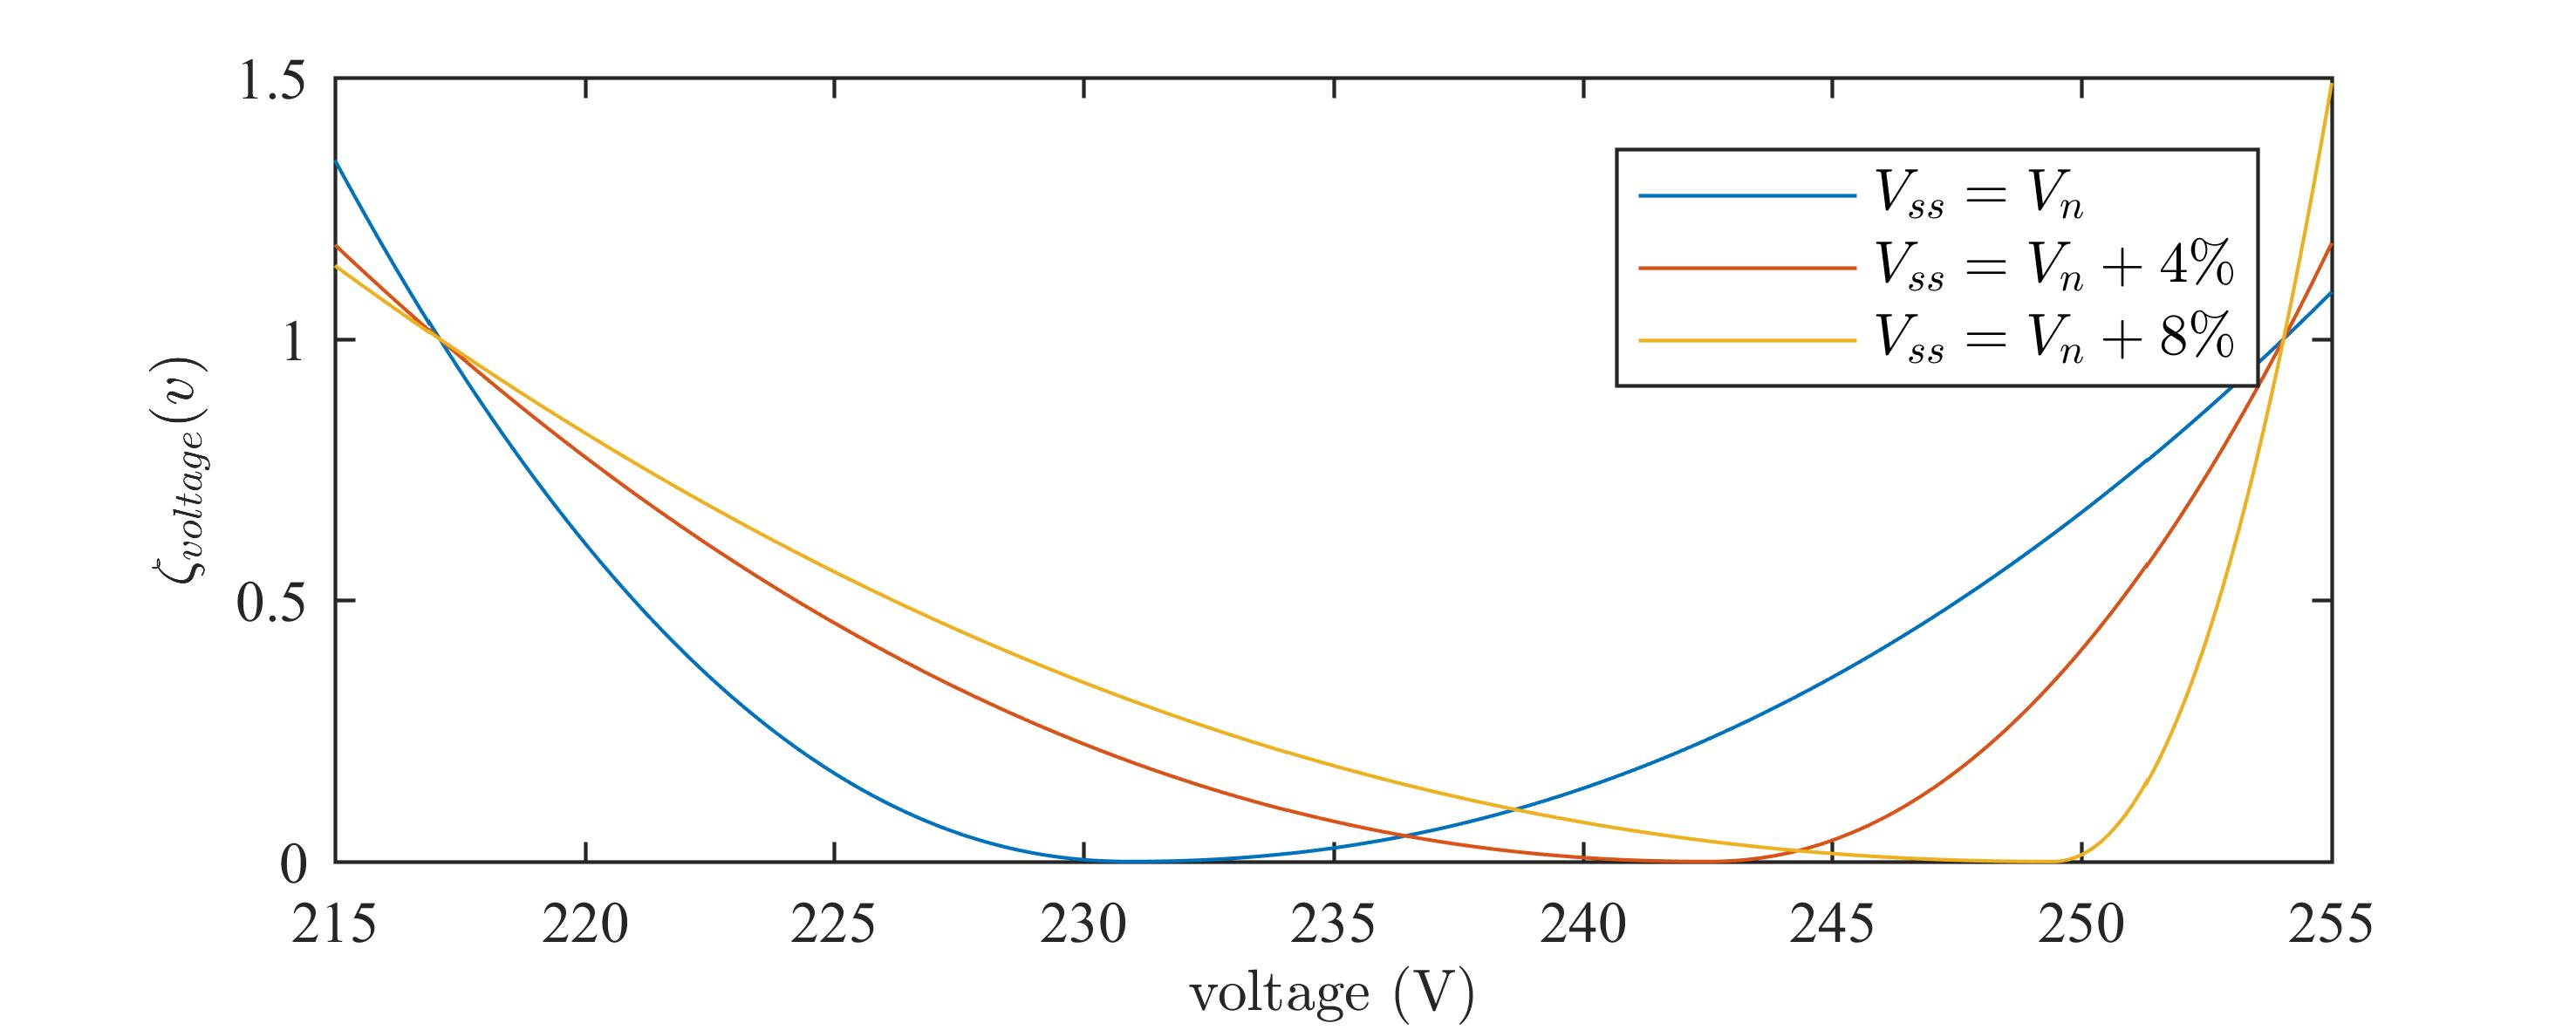
\includegraphics{_chapter1/fig/voltage-deviation}
	\caption{Cost function $\zeta_\text{voltage}(v_\phi)$ values for different substation voltages}	
	\label{ch1:fig:voltage-deviation}
\end{figure}

It can be seen that the cost at the high and low voltage thresholds equates to one, and to zero at the set substation voltage.
When boosting this voltage, $V_{ss}$, only the zero intersection is moved, whereas the high and low voltage crossings remain unchanged.
In Figure \ref{ch1:fig:voltage-deviation}, this behaviour is demonstrated by boosting $V_{ss}$ by +4\% and +8\%.

\subsection{Voltages at ESMU's PCC}
\label{ch1:subsec:voltages-at-esmu}

At the ESMU's PCC, it is connected to all three phases of the feeding cable.
The location of this PCC is at some distance from the substation or simply ``down stream'' the feeder.
Where to connect the ESMU, in order to achieve a best possible network impact, is explained in Section \ref{ch1:sec:data-and-network-models}.
Ignoring the exact ESMU location, voltage along the line, i.e. from the substation to its PCC, will change and most likely drop.
The reason behind this effect is due to resistive and inductive losses in the distribution lines.
These losses are amplified with proximity to the substation, since load currents are aggregated.
For purely consumptive loads, and particularly under heavy load conditions, this voltage may at some stage drop below the low-voltage threshold.
As mentioned in literature, this threshold is an operational constraint of LV networks and must not be violated to assure correct appliance operation and prevent financial penalisation.

In order to mitigate this voltage drop, power is injected into the feeder at the ESMU's PCC.
Doing so boosts the voltage at that location since the portion of the load current that would normally be supplied by the substation is now delivered by the ESMU.
The effect of this power injection is sketched in the figure below.

\begin{figure}\centering
	\subfloat[Voltage drop along feeder without ESMU intervention]{%
		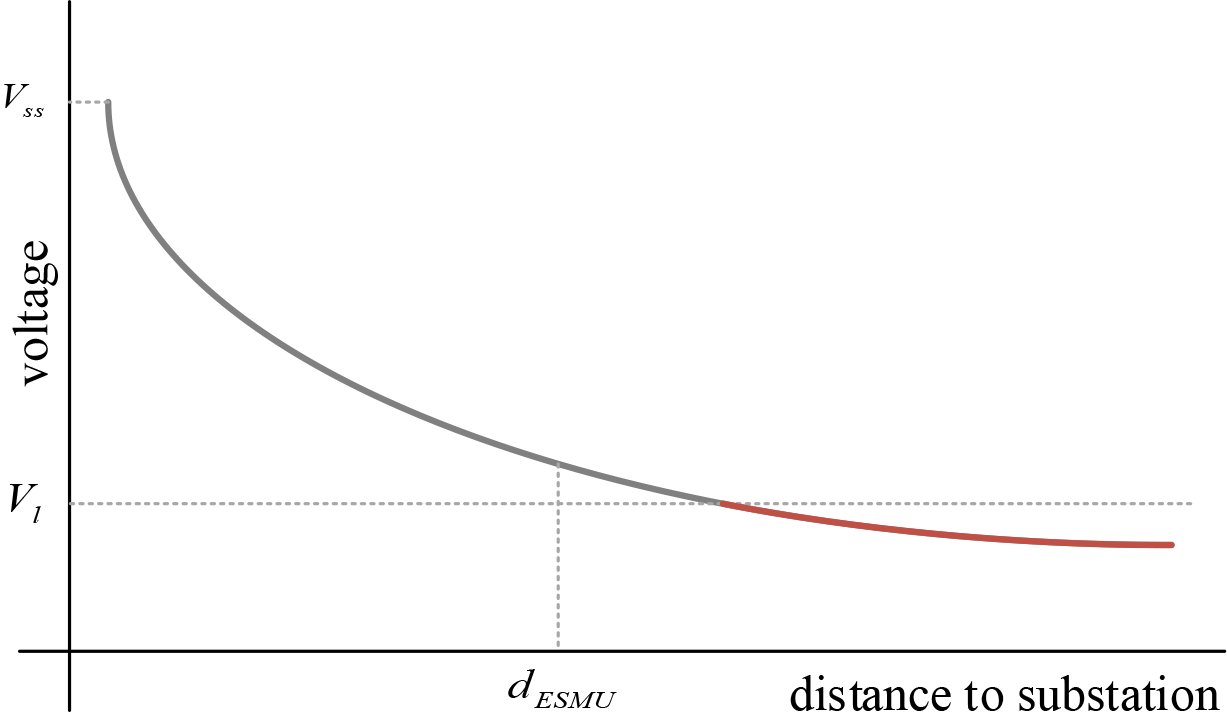
\includegraphics[width=0.45\textwidth]{_chapter1/fig/sketch-voltage-esmu-normal}%
		\label{ch1:subfig:sketch-voltage-esmu-normal}%
		}
	\hspace{5mm}
	\subfloat[Voltage drop along feeder with ESMU intervention]{%
		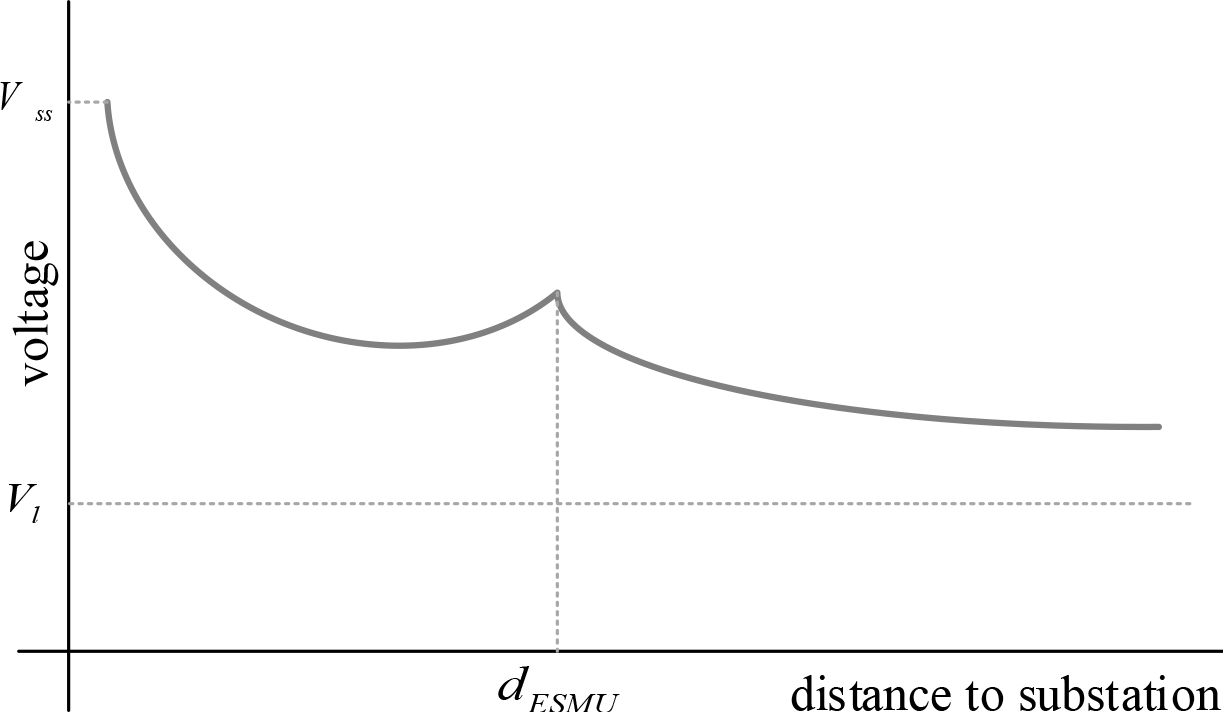
\includegraphics[width=0.45\textwidth]{_chapter1/fig/sketch-voltage-esmu-boost}%
		\label{ch1:subfig:sketch-voltage-esmu-boost}%
		}
	\caption{Benefits of ESMU power injection on the voltage drop along the feeder}
	\label{ch1:fig:sketch-voltage-esmu}
\end{figure}

In Figure \ref{ch1:subfig:sketch-voltage-esmu-normal}, an expected voltage drop along the feeder is sketched, where the down stream feeder section's voltage dropped below $V_l$.
In contrast, Figure \ref{ch1:subfig:sketch-voltage-esmu-boost} shows how the ESMU's intervention can alleviate some load and raise the trailing voltage levels to a level above $V_l$.

This realistic key network parameter is translated into a cost function, since the P2N voltage at the ESMU's PCC can be measured quite easily.
To do so, the three-phase PCC voltage, $\textbf{v}_{ESMU}(t)$ (where $v_{ESMU,p}(t) \in \textbf{v}_{ESMU}(t)$), is used in Equation \ref{ch1:equ:voltage-deviation}; the same cost used for the substation transformer's secondary voltage.
Therefore, the resulting cost can be formulated as $\zeta_\text{voltage}(\textbf{v}_{ESMU}(t))$.

\subsection{Voltages at customer laterals}
\label{ch1:subsec:voltages-at-customers}

As mentioned in Chapter \ref{ch-introduction:sec:overview}, the allowable voltage range at customers is defined by the Electricity Safety, Quality and Continuity Regulations (ESQCR).
Monitoring those voltages in real-time to assure they obey these regulations is costly, and therefore they are left unmonitored.
Ultimately, when it comes to voltage level correction, only substation voltage levels and customer voltage levels need to be controlled.
This fact is to assure proper transformer operation (e.g. to maximise its lifespan) and to prevent penalisation due to customer voltage violation (i.e. fining according to the ESQCR).
As explained in Section \ref{ch1:subsec:voltages-at-esmu}, ESMU can impact voltage levels for all customers but, as mentioned above, these voltage levels cannot be measured in reality.
In simulations however, all loads' voltages can be extracted with ease, which is why they are included but treated as theoretical key network parameters.

To illustrate this load voltage drop, a snapshot OpenDSS simulation was run on the IEEE LV Test Case with all load powers set to a high value of 8kW\footnote[1]{Whilst historic and recent loads may reach values of this magnitude quite seldom, future customer demand with the aggregated effect home-charging of EVs may indeed yield extreme scenarios like this.}.
In the following plot, the magnitude of the load bus voltages against the distance between the corresponding load and its feeding substation was drawn.

\begin{figure}\centering
	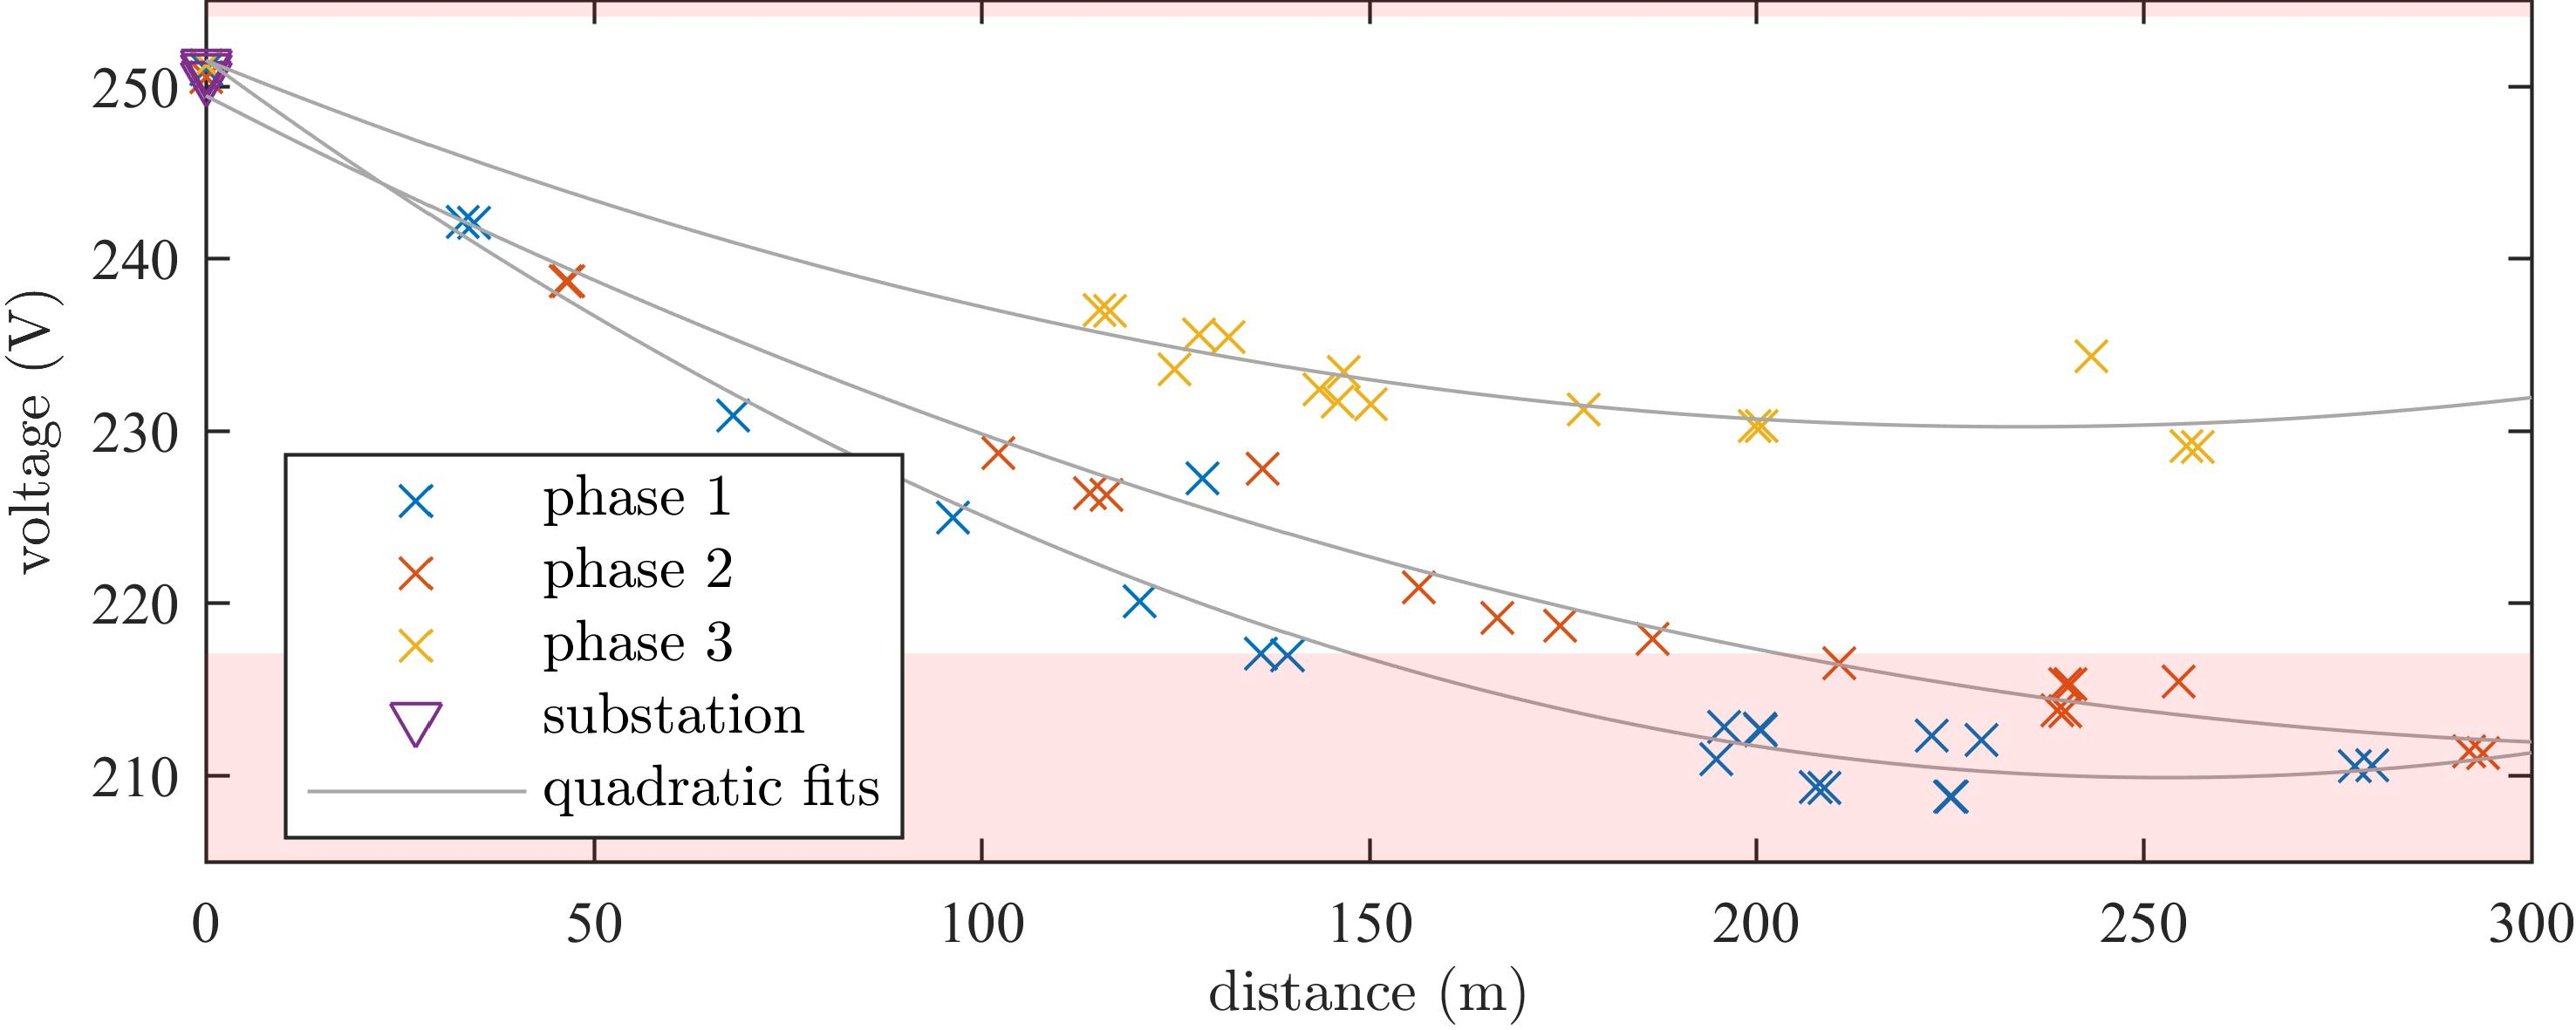
\includegraphics{_chapter1/fig/voltage-drop-for-loads-along-feeder}
	\caption{Voltage at the loads in the IEEE LV Test Case network for a total load of 440kVA against distance between the corresponding load and substation: for the quadratic fit $R^2=58.76\%$}
	\label{ch1:fig:voltage-drop-for-loads-along-feeder}
\end{figure}

In this Figure \ref{ch1:fig:voltage-drop-for-loads-along-feeder}, two observations can be made.
For one, it can be seen that phases are significantly unbalanced.
Secondly, customers further than 200m from the substation experience low-voltage events (for this particular scenario).
As already proposed in the previous section, ESMU aims to avoid these voltage violations, but the number of loads would add significant computational burden on the any used solving algorithm.

To address this problem, the previously defined voltage cost function (i.e. Equation \ref{ch1:equ:voltage-deviation}) is expanded.
Rather than including the cost for every single customer's voltage deviation, only the worst deviation is used.
By limiting this number, solvers need not consider such a large number of parameters and only focus on the worst network parameter.
This focus is of particular need if the impact of the ESMU on some customers' voltages is relatively low, since the aggregate cost would otherwise cloud the impact on those individual voltages.
For this work, the customer (or load) voltage is defined as $\textbf{v}_{load}(t)$ (where $v_{load,i,p} \in \textbf{v}_{load}$) and used in the new cost function, $\zeta_\text{load voltage}(\textbf{v}_{load}(t))$, as such:

\begin{equation}
\begin{split}
	\zeta_\text{load voltage}(\textbf{v}(t)) := \max_{i,\phi}{\zeta_\text{voltage}(v_{i,p}(t))} \\
	\text{ where } i \in \{1, \dots I\} \text{ and } \phi \in \{1, \dots, \Phi\} \text{ and } I \in \mathbb{Z}_{>0} \text{ and } \Phi \in \mathbb{Z}_{>0}
\end{split}
\label{ch1:equ:load-voltage-deviation}
\end{equation}

\subsection{Total power flow}
\label{ch1:subsec:total-power-flow}

Beside having to keep voltages within their specified operational boundaries, DNOs want to make sure that the distribution network operates in an efficient and ideal manner.
Determining how ideal a three-phase network operates can be done by e.g. assessing the balance of the network's phases.
The frequently neglected disturbance of unbalanced phases may not have an immediately associated impact on the network's customers, but the negative long term effects (e.g. the effects of asymmetric load on transformers and rotating machones) must not be neglected since they weaken the network's infrastructure.
The choice of how to connect customers to the LV feeder makes phase unbalance a dominant problem in the UK.
Customers in urban UK distribution networks have a single-phase link to the three-phase feeder line.
The link is established by connecting their supply cables or ``laterals'' between a phase and the neutral conductor.
In the UK, the phase allocation for each customer has been random, in order to distribute load as evenly as possible across all three phases.
In theory, this approach should assure a more or less balanced three-phase load, yet in reality this is not the case.
Even if the number of customers on each phase was the same for all three phases, the probability that all customers' load profiles are identical is very low.
Therefore, the likeliness of LV distribution feeders in the UK to be unbalanced is very high.

Since substation monitoring is capable of providing three-phase power measurements, they are used as realistic key network parameters, and summarised in a substation power vector $\textbf{s}_{ss}(t)$.
Deriving phase unbalance from these three-phase sub is done by following the American National Standards Institute (ANSI) definition of phase unbalance \cite{ANSI-MB-1-2011}.
The standardised Unbalance Factor (UF) is defined as:

\begin{equation}
	\text{UF}(\textbf{x}) := \frac{\max_n |\bar{\textbf{x}} - x_n|}{\bar{\textbf{x}}}
	\label{ch1:equ:unbalance-equation}
\end{equation}

Here, $\textbf{x}$ is a three phase vector, where $x_n \in \textbf{x} \text{ for } n=[1, 2, 3]$.
$x_n$ may be a voltage, current or power measurement per phase, but for context of this work $x_n$ was chosen to be the power flow into the network.
For clarity, the notation $\bar{\textbf{s}}$ is used to define the mean of all three phase values.
The mean's definition is give below:

\begin{equation}
	\bar{\textbf{x}} := \frac{1}{3}\sum_n^3{x_i}
\end{equation}

From the substation monitoring, a three-phase substation power vector, $\textbf{s}_{ss}(t)$ (where $s_{ss,p} \in \textbf{s}_{ss}$), is used and the network's phase unbalance can be calculated.
Since this forms another realistic key network parameter, the UF in Equation \ref{ch1:equ:unbalance-equation} was formulated into a cost function, too.
The resulting cost function $\zeta_\text{unbalance}(\textbf{s}_{ss})$ is defined as:

\begin{equation}
	\begin{split}
		\zeta_\text{unbalance}(\textbf{s}(t)):=&\text{UF}(\textbf{s}(t)) - 1 \forall t\\
		=&\frac{\max_p\left|\overline{\textbf{s}(t)} - s_{p}(t)\right|}{\overline{\textbf{s}(t)}} \forall t\\
		=&\frac{\max_p\left|\left(\frac{1}{P}\sum_p^P{s_{p}(t)}\right) - s_{p}(t)\right|}{\frac{1}{P}\sum_p^P{s_{p}(t)}} \forall t\\
		&\text{where } p \in [1, 2, \dots P]
	\end{split}
	\label{ch1:equ:unbalance-cost}
\end{equation}


The minimum value of $\text{UF}(\textbf{s}_{ss})$ is one.
Therefore an adjustment was required so that a perfectly balance network would result in an $\text{UF}(\textbf{s}_{ss})$ of zero.
An illustration how this cost function is provided in the figure below.

\begin{figure}\centering
	
\includegraphics[width=5cm]{foo}
	\caption{Sample network imbalance for different phase loadings as defined in ANSI/NEMA MG 1-2011}
	\label{ch1:fig:power-unbalance}
\end{figure}

Here, it can be seen how $\zeta_\text{unbalance}(\textbf{s})$ varies with an increasing separation of the three phases' power values.

\subsection{Substation line utilisation}
\label{ch1:subsec:substation-line-utilisation}

Although phase unbalance deteriorates the efficiency and life expectancy of three-phase network assets, high power demand puts strain on the physical cables themselves.
This is due dominantly due to resistive and inductive losses heating the cables, and bringing them closer to their operational limits.
Therefore, cables have an assigned thermal rating which must not be exceeded to prevent permanent cable damage or network failures.
At substation level, to prevent over-currents, fuses or reclosers are installed that will disconnect the network under fault or high demand conditions.
To quantify whether the substation fuse is approaching its tripping point, its nominal rating is used as reference.

For the context of this work, this nominal fuse rating, $i_{fuse}$, is a fixed value for the fuse at the substation and must not be exceeded.
Using the three-phase current vector from substation monitoring, $\textbf{i}_{ss}(t)$ (where $i_{ss,p}(i) \in \textbf{i}_{ss}(t)$) a cost function, $\zeta_\text{fuse utilisation}(\textbf{i}_{ss}(t))$, can be defined as follows:

\begin{equation}
	\zeta_\text{fuse utilisation}(\textbf{i}(t)) :=%
	\left|\frac{\sum_{\phi=1}^{\Phi}{i_\phi(t)}}{I_\text{fuse}}\right|^2%
	\text{ where } \phi \in \{1, \dots, \Phi\}%
	\text{ and } \Phi \in \mathbb{Z}_{>0}
	\label{ch1:equ:fuse-utilisation}
\end{equation}

A plot has been included in the below figure, which illustrates how this quadratic cost behaves as substation current increases.

\begin{figure}
	
\includegraphics[width=5cm]{foo}
	\caption{Cost of line or fuse utilisation against network current}
	\label{ch1:fig:fuse-utilisation}
\end{figure}

For this simple case, the substation line rating was set as $i_{fuse}=400\text{A}$, and the total substation current is the sum of all three phase currents.

\subsection{Maximum line utilisation}
\label{ch1:subsec:maximum-line-utilisation}

Similar how voltage levels at all customers are theoretical key network parameters, currents in all lines are key network parameters, too.
Optimising the aforementioned current at substation level would prevent unintentional feeder disconnection and equipment damage, yet lines' ratings impose distributed limits, too.
Moreover, as feeder cables are not of a singly type of cable.
For instance, the main three-phase wire must to be sufficiently scaled to deliver several 100s of Amperes to a collection of customers, whilst branches with a few loads may only experience 10s of Amperes worth of current.
Furthermore, as distance to the substation increases, fewer customers are connected down stream, which allows the feeding cables to be down scaled, too.
This network topology is very common for radial distribution networks, since it saves significant equipment cost without compromising the network integrity.
Yet with the advent of DG and electrified LTCs, the feeder's branches are going to experience larger current flows.

This is why the previous cost function, as it was defined in Equation \ref{ch1:equ:fuse-utilisation}, ought to be expanded to take all line currents and ratings into account.
Since this work was based on network simulations, each line current, $i_{line,l,p}(t)$ (where $l$ represents the line number and $p$ the phase in that line), could be extracted with ease.
Collecting them in $\textbf{i}_{line}(t)$ (where $i_{line,l,p}(t) \in \textbf{i}_{line}(t)$) allows the formulation of an extended line utilisation cost function, $\zeta_\text{line utilisation}(\textbf{i}_{line}(t))$, which is defined as:

\begin{equation}
\begin{split}
	\zeta_\text{line utilisation}(\textbf{i}(t)) :=
	\max_{l}{\left(\frac{\sum_{\phi=1}^{P}{i_{l,\phi}(t)}}{I_{\text{nom},l}}\right)^2} \\
	\text{where } l \in \{1, \dots, L\} \text{ and } \phi \in \{1, \dots, \Phi\} \text{ and } L \in \mathbb{Z}_{>0} \text{ and } \Phi \in \mathbb{Z}_{>0}
\end{split}
\label{ch1:equ:line-utilisation}
\end{equation}

In this quadratic cost function, $i_{nom,l}$ is the nominal rating of line $l$ in the network.
Also, and similar to Equation \ref{ch1:equ:load-voltage-deviation}, by considering only the maximum line utilisation, computational burden is reduced whilst parameter dependent sensitivity is increased.

\subsection{Distribution losses}
\label{ch1:subsec:losses}

When it comes to profit margins, energy losses in a distribution network are unwanted, since nobody pays for undelivered energy.
Although the losses a single distribution network are small in comparison to the losses in the entire electricity grid, the aggregate effect of reducing those losses could have a noticeable impact.
To put this into perspective, the losses in the IEEE LV Test Case network were 58kW, when simulated under the same high demand scenario which was used for voltage drop visualisation in Section \ref{ch1:subsec:voltages-at-customers}.
This equates to 12\% of the total network demand ($\text{i.e. }\frac{s_{losses}(t)}{\sum_{p=1}^P{s_{ss,p}(t)}} \approx \frac{58kW}{484kW}$).
Since this is a high network load, losses would be noticeably lower for notmal network operation.
This is made apparent in Figure \ref{ch1:fig:losses-against-network-demand}, where the uniform network load is varied and the corresponding losses are plotted against this variation.

\begin{figure}\centering
	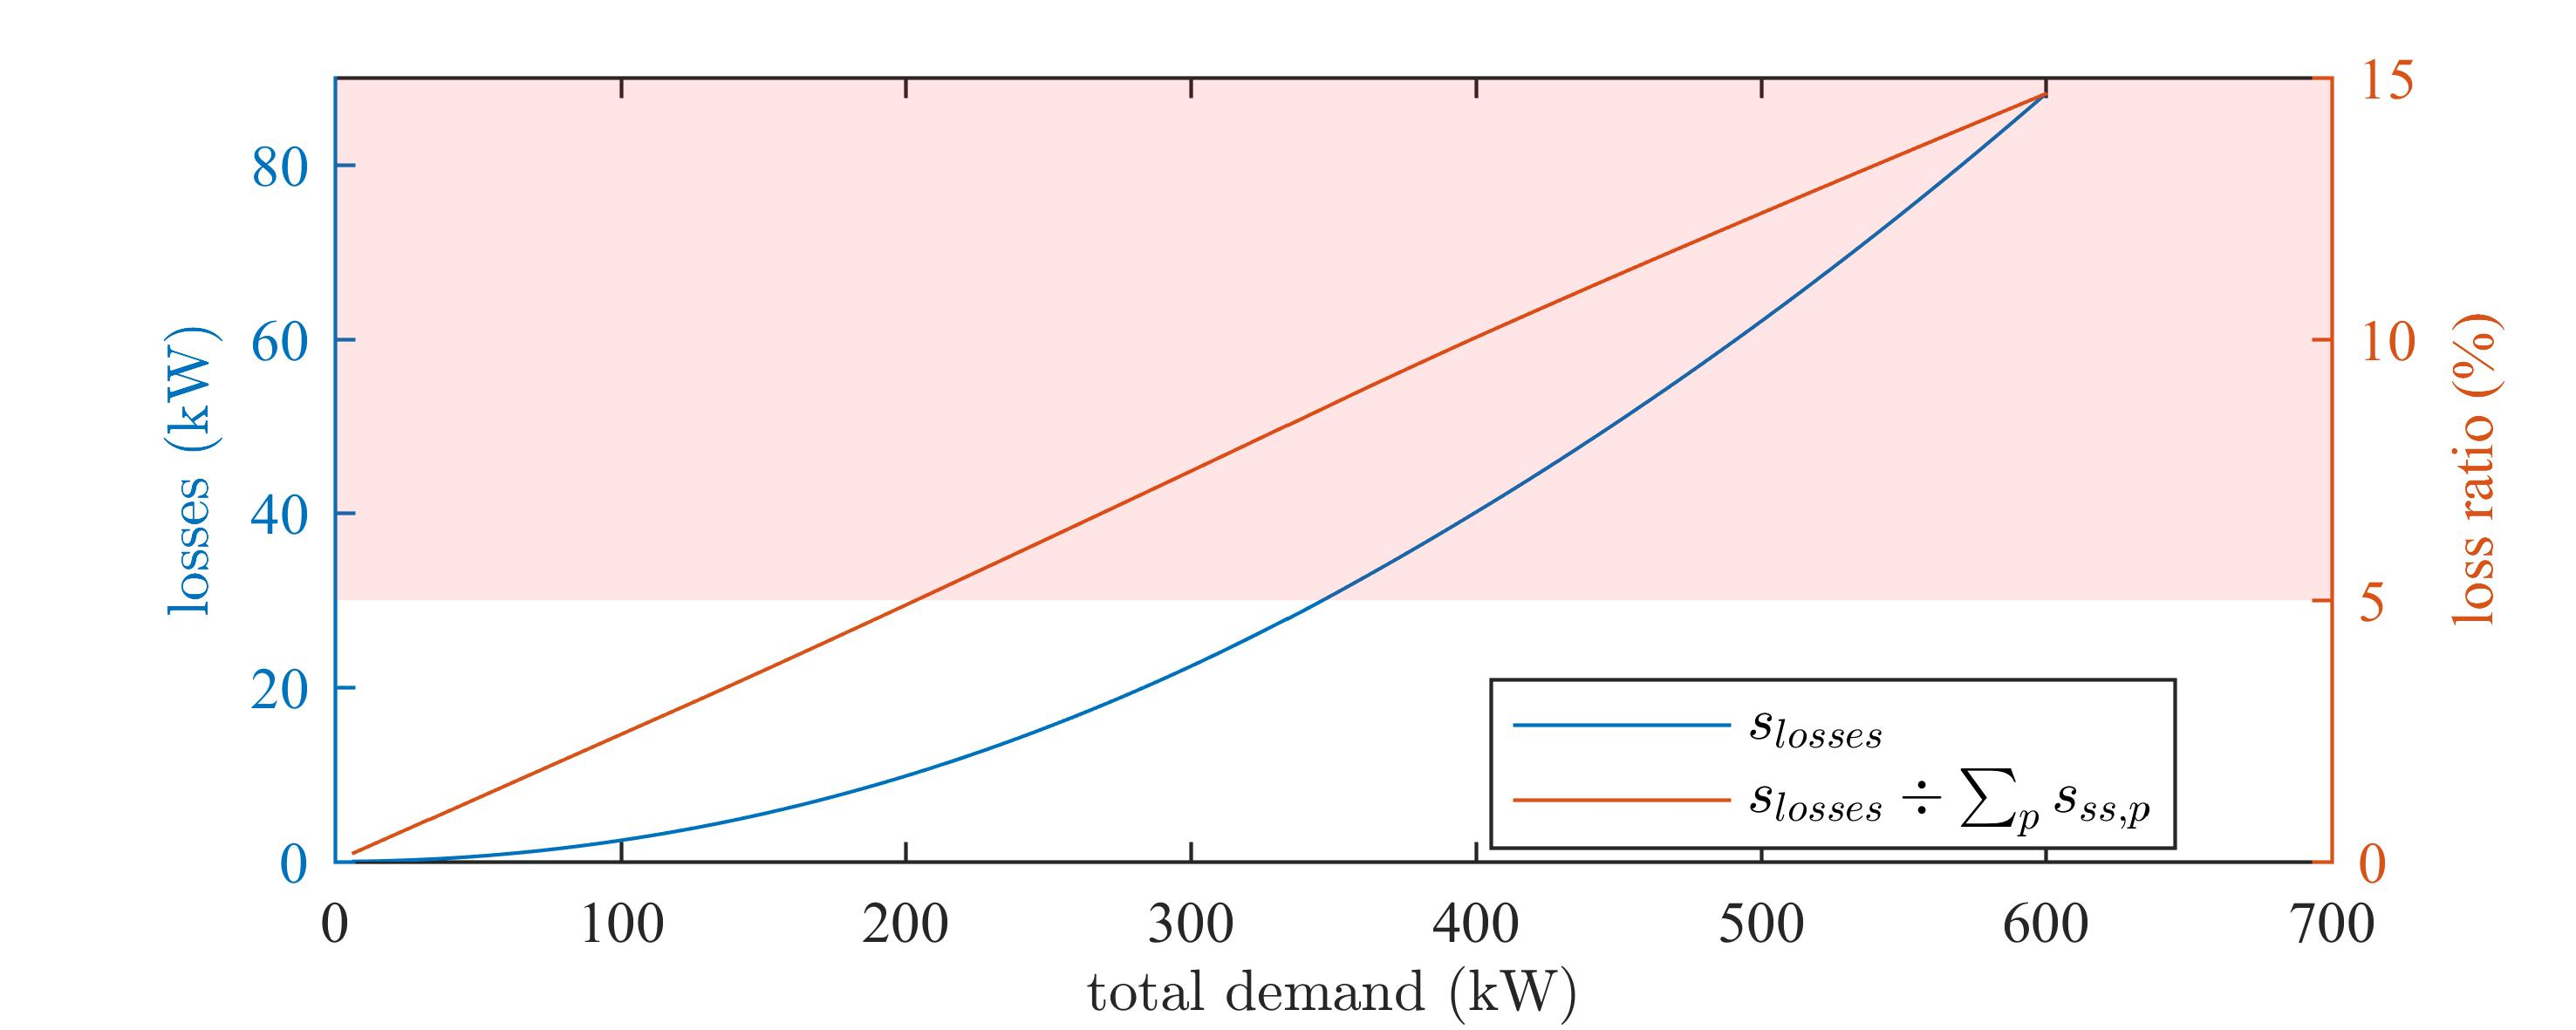
\includegraphics{_chapter1/fig/losses-against-network-demand}
	\caption{Losses against increasing power demand}
	\label{ch1:fig:losses-against-network-demand}
\end{figure}

In Figure \ref{ch1:fig:losses-against-network-demand}, the region where losses exceed 5\% of the total network power is highlighted in red.
These preliminary results were found from power flow simulations.
In reality however, losses cannot be determined this easily.
Therefore, the network losses, $s_{losses}(t)$, are seen as theoretical key network parameters and used in the final cost function $\zeta_\text{losses}(s_{losses}(t))$, which is simply defined as:

\begin{equation}
	\zeta_\text{losses}(s(t)) := |s(t)| 
	\label{ch1:equ:losses}
\end{equation}



\section{Network, Data and Battery Models}
\label{ch1:sec:data-and-network-models}

All key network parameters and their associated cost functions have now been established.
In this section the network model and power flow simulation, from which all aforementioned key network parameters were extracted are explained.
Also, all data that is used throughout the presented research is included, too.

\subsection{Standardised Network Model}
\label{ch1:subsec:standardised-network-model}

The IEEE Power and Energy Society (IEEE-PES) provided several multi-node test feeder cases.
These test cases used to be limited to distribution networks in the United States.
In 2015 however, they published a standardised model of a LV distribution network for the UK power network.
This model is called the ``European Low Voltage Test Feeder'' and an OpenDSS compatible version can now be obtained from their website \cite{DistributionTestFeeders2017}.
Within the context of this work, this feeder is referred to as the ``LV Test Case'' and a network plot of this feeder has been included for reference.

\begin{figure}\centering
	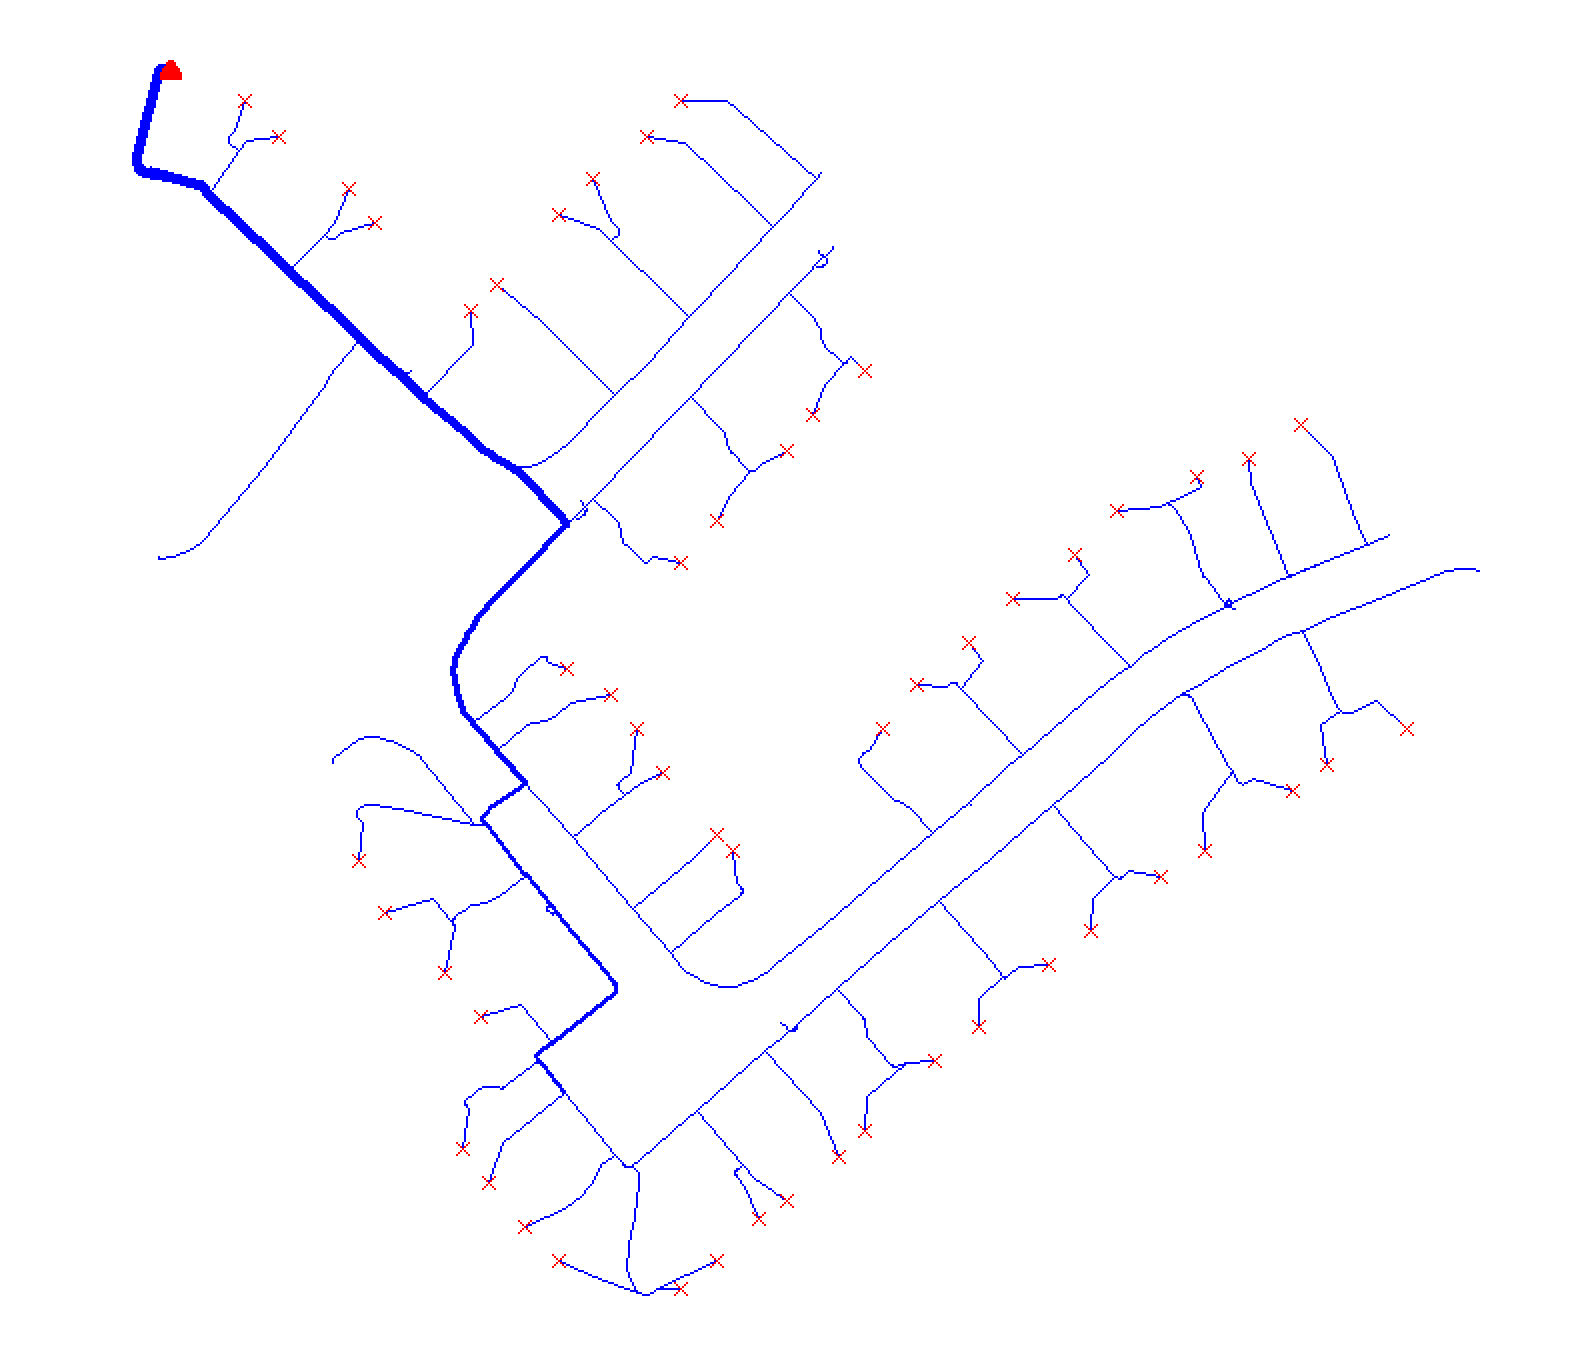
\includegraphics[width=0.8\textwidth]{_chapter1/fig/network-plot-LVTestCase}
	\caption{A power flow plot of the IEEE-PES European Test Case Feeder, i.e. a LV distribution network in the UK.}
	\label{ch1:fig:network-plot-LVTestCase}
\end{figure}

Here, a substation (triangle in north west) provides power to the feeder, and the power flowing through this feeder is visualised by the thickness of its lines.
In total, there are 55 single-phase households connected to the substation, which represents a medium-sized UK feeder.

\subsection{Load Profiles: Minutely and Half-Hourly}

Alongside the LV Test Case, 100 minutely demand profiles were supplied; each profile being 24h long.
Therefore, by assigning one load profile to each customer, a series of 1440 snapshot simulations could be run in OpenDSS in order to simulate the variation and volatility in demand over the entire day.
Since the provided power values only provided active power values, a standardised power factor of 0.95 was used for all loads to calculate their reactive component.
This non-unity power factor simulates a certain inductive load, which would otherwise be neglected.

\nomenclature{$s_\text{net}(t)$}{Apparent network load at time $t$ (Chapter \ref{ch1})}
\nomenclature{$s_{\text{load},i}(t)$}{Apparent load power for load $i$ at time $t$, where $s_{\text{load},i}(t) \in \textbf{s}_\text{load}(t)$ (Chapter \ref{ch1})}
\nomenclature{$\textbf{s}_\text{load}(t)$}{Apparent load power vector of all loads at time $t$ (Chapter \ref{ch1})}

Before any scheduling could take place, the total network load, $s_\text{net}(t)$, had to be calculated by aggregating all customer loads:

\begin{equation}
	s_\text{net}(t) := \sum_{i=1}^{I} s_{\text{load},i}(t)
	\text{ where } I \in \mathbb{Z}_{\geq 0}
\end{equation}

This demand is however at minutely resolution.
Computing the ESMU schedule at this resolution (or any sub-half-hourly resolution) for an entire day is very computationally demanding and highly ineffective.
Mainly, since cutting edge research in load forecasting has shown that demand variability due to behavioural unpredictability makes forecasting at high temporal resolution unfeasible, but also since traditional forecasts are generally provided at half-hourly resolution.
Therefore, the sub-half-hourly profile had to be down-sampled or extrapolated to a coarser resolution, by using a synchronisation function $k(t)$.
This function links the original sub-half-hourly to a resulting half-hourly time-series like so:

\begin{equation}
	k(t) := \left\lfloor\frac{t-1}{K\Delta t}\right\rfloor+1
	\label{ch1:equ:synchronisation-function}
\end{equation}

\nomenclature{$\Delta t$}{Sampling period , where $\Delta t \in \mathbb{Z}^{>0}$ (Chapter \ref{ch1})}
\nomenclature{$K$}{Number of blocks to downsample the sub-half-hourly profile into, where $K \in \mathbb{Z}^{>0}$ and $\frac{T_\text{sch}}{K} \in \mathbb{Z}^{>0}$ (Chapter \ref{ch1})}
\nomenclature{$k(t)$}{Synchronisation function used to downsample the sub-half-hourly profile (Chapter \ref{ch1})}
\nomenclature{$k$}{Half-hourly timing, where $k \in [1, \dots, K]$ (Chapter \ref{ch1})}
\nomenclature{$T_\text{sch}$}{Scheduling horizon, where $T_\text{sch} \in \mathbb{Z}^{>0}$ (Chapter \ref{ch1})}

Here, $\Delta t$ is the sampling period (i.e. minutely period) of the simulation, and $K$ is number of low-resolution blocks.
It should be noted that the integer multiple of $K$ has to equate to the scheduling horizon's length, $T_\text{sch}$; i.e. $T_\text{sch} \overset{!}{=} \alpha K \text{ where } \alpha \in \mathbb{Z}^{>0}$.
Only in this case can the sub-half-hourly profile be divided into a complete set of chunks, where each chunk is of length $K\Delta t$.
Therefore, the resulting half-hourly network load, $s^{*}_\text{net}(t)$, can be defined as follows:

\begin{equation}
	s^*_{network\;\;load}(t^*) = \frac{T^*}{T}\sum_{t=1}^{\frac{T}{T^*}}s_{network\;\;load}\left(\frac{T}{T^*}(t^*-1) + t\right) \forall t^* \text{ where } t^* \in [1, \dots, T^{*}]
	\label{ch1:equ:down-sampling-to-half-hourly}
\end{equation}

Since all power values from a period of $k(t)K \rightarrow (k(t)+1)K-1$ are equal, a simplified half-hourly power vector is introduced as $p_\text{net}(k)$. 
In this and any subsequent vector, half-hourly timing is indicated by using the half-hourly time $k$ instead of the sub-half-hourly time $t$, where $k \in [1, \dots, K]$ and $K \in \mathbb{Z}^{>0}$.
The link between $s^{*}_\text{net}(t)$ and $s_\text{net}(k)$ is therefore defined as:

\begin{equation}
	s_\text{net}(k) := s^{*}_\text{net}(Kk) \forall k
	\label{ch1:equ:half-hourly-power-profile}
\end{equation}

It is worth mentioning, that from here on all subsequent cost functions (i.e. any $\zeta$) that deal with half-hourly profiles, are functions that use the half-hourly timing $k$, whilst sub-half-hourly or real-time costs use the high-resolution timing $t$.
This difference will become important when differentiating between scheduling costs and the aforementioned network costs (which are based on a set of key network parameters).
Nonetheless, to illustrate how the original sub-half-hourly network load is extrapolated into the resulting half-hourly demand, both profiles are plotted in a figure below.

\begin{figure}\centering
	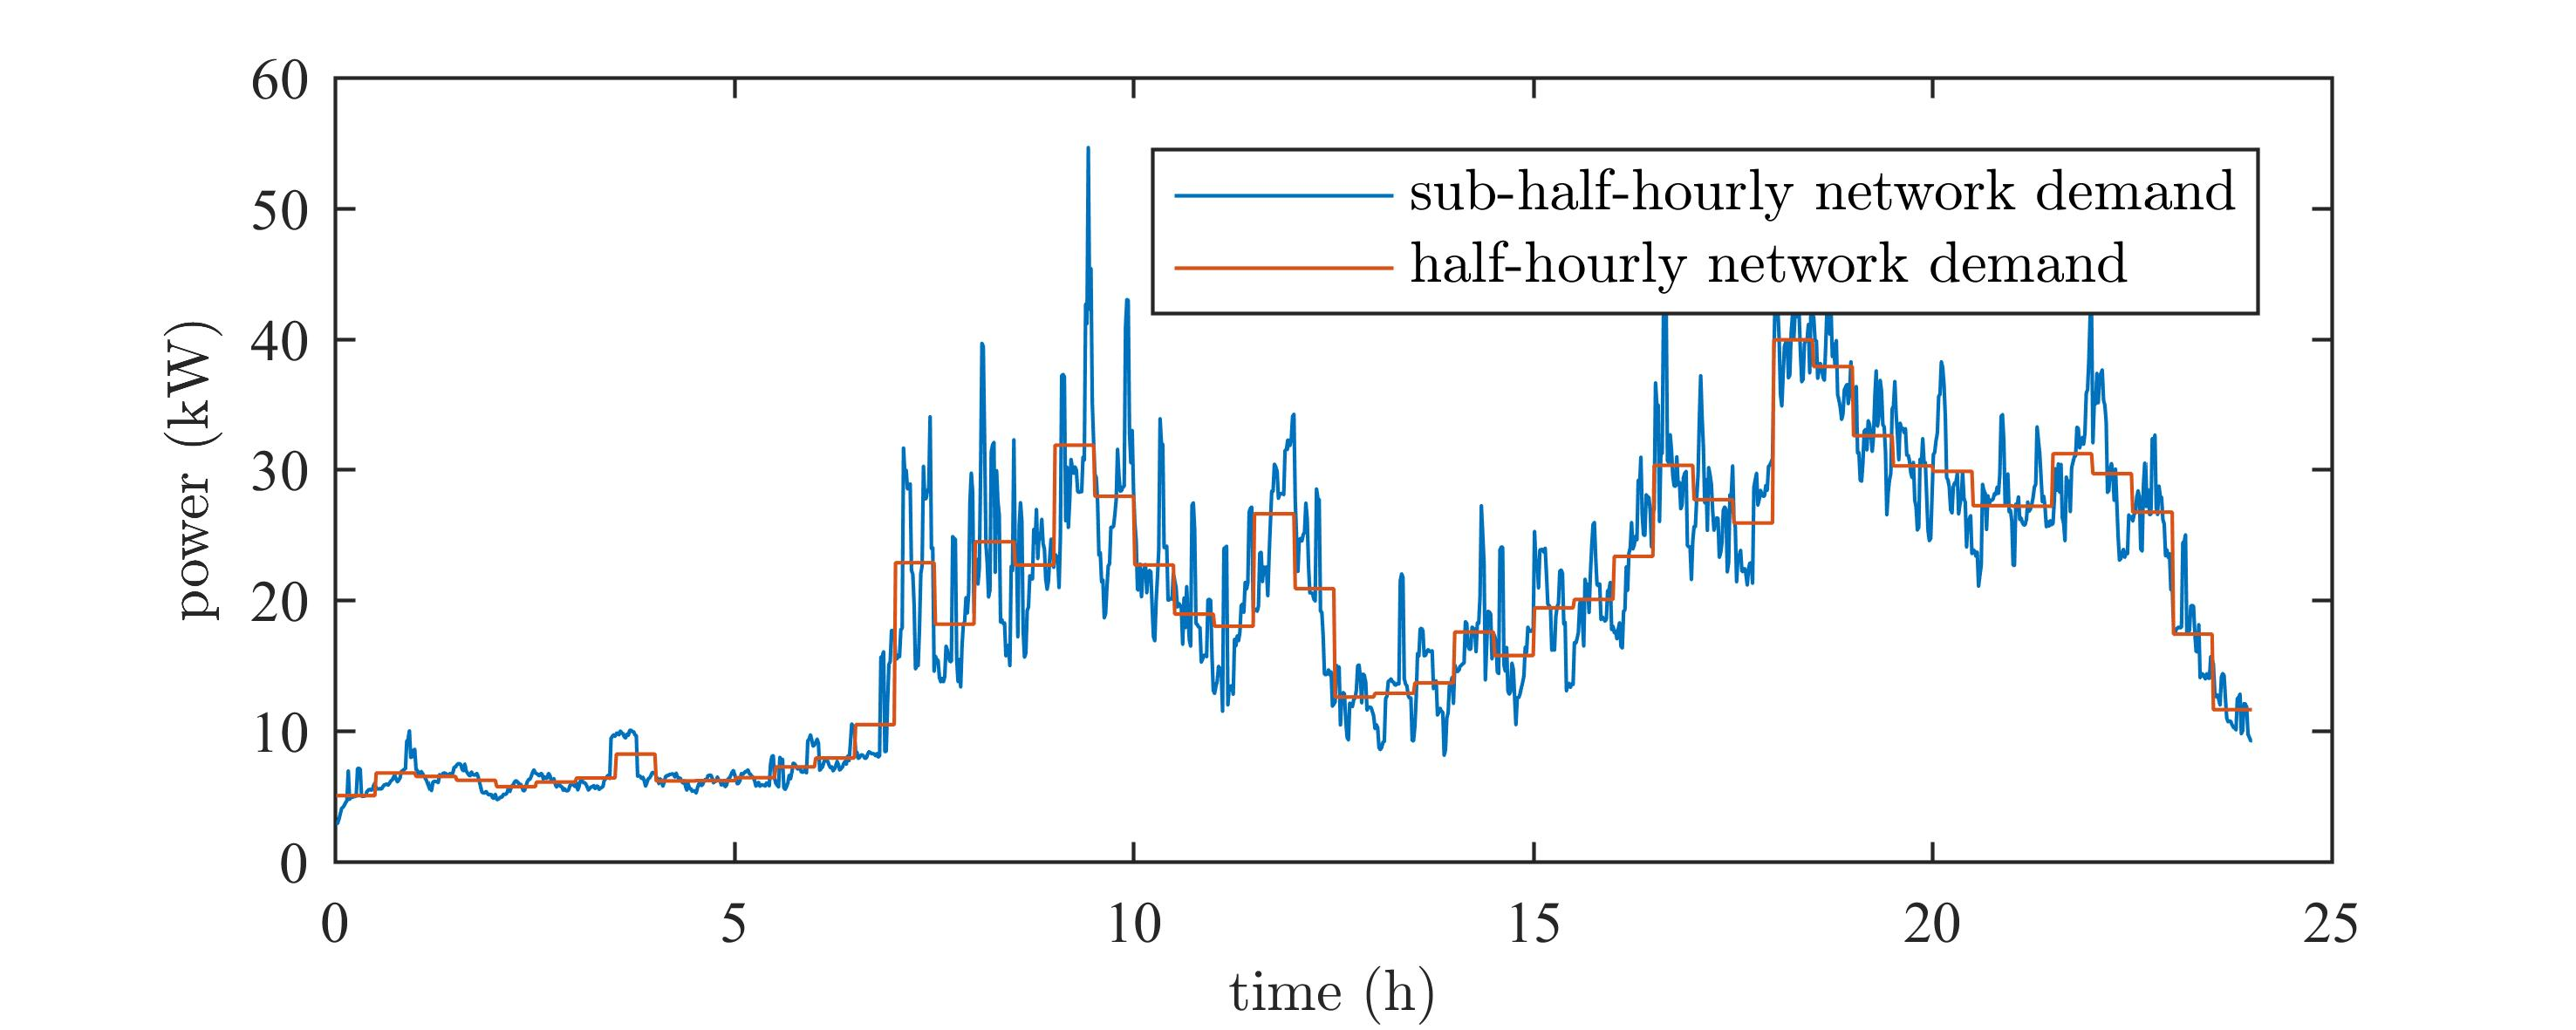
\includegraphics{_chapter1/fig/sub-half-horuly-demand-comparison}
	\caption{Highly variable and volatile demand profile vs half-hourly demand (i.e. a forecast under perfect foresight conditions)}
	\label{ch1:fig:sub-half-horuly-demand-comparison}
\end{figure}

In Figure \ref{ch1:fig:sub-half-horuly-demand-comparison}, it can be observed how the high variability and volatility in power is removed in the half-hourly profile.
When generating the ESMU schedules (which is addressed in Section \ref{ch1:subsec:esmu-schedule-generation}) these variations are neglected and the unwanted peak power demands are hence no longer sufficiently compensated.

\subsection{Battery Model}

\nomenclature{$S_\text{rating}$}{Rating of battery's power electronics, where $S_\text{rating} \in \mathbb{R}^{>0}$ (Chapter \ref{ch1})}

The ESMU systems that were deployed throughout the NTVV project consisted of two parts: the Power Management Unit (PMU) and the Energy Storage Unit (ESU).
The PMU controls the three-phase powers and links the ESU to the grid.
Each PMU's per phase power rating, $S_\text{rating}$, is 12kVA and, beside battery charging and discharging, can also perform filtering functions, e.g. compensating for harmonic distortion, reactive power and phase unbalance.
The ESU is a modular container of 12.5kWh of Li-Ion energy storage that can be aggregated to increase the total energy storage capacity.
All battery monitoring, conditioning and regulation is performed within the ESU and hence need not be considered for the scope of this work.
However, control instructions that are sent to the ESMU system should not request the device to operate outside its own specifications, i.e. under- or over-charge the batteries.

In order to simulate this ESMU system and its energy storing behaviour, a model is developed from the given device specifications.
This model includes both an charge-discharge efficiency and standby losses.
The charge-discharge efficiency is related to the efficiency of the PMU's power converters, which are quoted to have a round trip efficiency of 98\%.
The standby losses on the other hand are associated to the nominal power drawn by the battery's control system as well as the battery's self-discharge rate.
It became common practice to assess the energy storage's charge level as the State of Charge (SOC) instead of using the actual charge stored.
This SOC is defined as:

\begin{equation}
	SOC(t) := \frac{E_{battery}(t)}{C_{battery}} \forall t
	\label{ch1:equ:state-of-charge-definition}
\end{equation}

\nomenclature{$C_\text{bat}$}{Battery capacity, where $C_\text{bat} \in \mathbb{R}^{>0}$ (Chapter \ref{ch1})}
\nomenclature{$E_\text{bat}(t)$}{Energy stored in battery at time $t$, where $E_\text{bat}(t) \in \mathbb{R}^{>0}$ (Chapter \ref{ch1})}
\nomenclature{$\eta$}{Round-trip efficiency of power electronics, where $\eta \in (0, 1]$ (Chapter \ref{ch1})}
\nomenclature{$s_{\text{bat},\phi}(t)$}{Single-phase apparent battery power for phase $\phi$ at time $t$, where $s_{\text{bat},\phi}(t) \in \textbf{s}_\text{bat}(t)$ (Chapter \ref{ch1})}
\nomenclature{$s_{\text{ESMU},\phi}(t)$}{Single-phase apparent ESMU power for phase $\phi$ at time $t$, where $s_{\text{ESMU},\phi}(t) \in \textbf{s}_\text{ESMU}(t)$ (Chapter \ref{ch1})}


SOC is therefore defined for any given time $t$, as the actual energy stored in the ESU, $E_\text{bat}(t)$, divided by the total capacity of the system, $C_\text{bat}$.
With the conversion efficiency as the factor $\eta$, the battery charge and discharge power, $s_\text{bat}(t)$ (in kW)\footnote[1]{It is worth mentioning, that $s$ is chosen for apparent power (i.e. active and reactive power in kVA), yet $s_\text{bat}$ is purely active (i.e. in kW).}, can be calculated for any given ESMU power, $\textbf{s}_\text{ESMU}(t)$ (where $s_{\text{ESMU},\phi}(t) \in \textbf{s}_\text{ESMU}(t)$).

\begin{equation}
\begin{split}
	s_\text{bat}(t) = 
	\begin{cases}
		\eta\text{Re}\left\{\sum_{\phi=1}^{\Phi}s_{\text{ESMU},\phi}(t)\right\} &\text{ if } \text{Re}\left\{\sum_{\phi=1}^{\Phi}s_{\text{ESMU},\phi}(t)\right\} \geq 0\\
		\frac{1}{\eta}\text{Re}\left\{\sum_{\phi=1}^{\Phi}s_{\text{ESMU},\phi}(t)\right\} &\text{ otherwise}
	\end{cases} \forall t \\
	\text{and } \phi \in [1, \dots, \Phi] \text{ and } \Phi \in \mathbb{Z}^{>0}
\end{split}
\label{ch1:equ:battery-power-definition}
\end{equation}

\nomenclature{$C_f$}{Charge factor or ``C-factor'' of the battery, where $C_f \in \mathbb{R}^{>0}$ (Chapter \ref{ch1})}

Although the ESMU's PSU rating, $S_\text{rating}$, may allow for a maximum power consumption of 36kVA (i.e. $=3\times12\text{kVA}$), the charging power is internally limited, due to a charging factor, $C_f$, which was chosen to be the standard value of 1.6.
This factor is the ratio between the battery's maximum discharge power and its total capacity (i.e. $s_\text{bat}(t) \leq C_f \cdot C_\text{bat} \forall t$).
Assuming that this charge/discharge power is applied and remains constant during a sample period of $\Delta t$, an equation describing the change in stored energy can be formulated.

\begin{equation}
	\Delta E_{battery}(t) = s_{battery}(t)t_s \forall t
	\label{ch1:equ:change-in-energy}
\end{equation}

\nomenclature{$\mu$}{Self-discharge losses of battery, where $\mu \in (0, 1]$ (Chapter \ref{ch1})}
\nomenclature{$\Delta E_\text{bat}(t)$}{Change in stored energy at time $t$ (Chapter \ref{ch1})}
\nomenclature{$SOC(t)$}{State of charge at time $t$ (Chapter \ref{ch1})}

As already mentioned, the energy level is however affected by standby losses, which are captured by a self-discharge factor, $\mu$.
Therefore, when adding the change in energy level to the current energy level in order to calculate the next energy level, this factor needs to be taken into account.

\begin{equation}
	E_{battery}(t+1) = \mu\left(\Delta E_{battery}(t) + E_{battery}(t)\right)
\label{ch1:equ:next-energy}
\end{equation}

In an ideal case, $\mu = 1$, where no energy would be lost in the storage system.
Finally, by adding the current energy level to the change in energy level, and by substituting Equation \ref{ch1:equ:state-of-charge-definition}, the next SOC can be found:

\begin{equation}
	SOC(t+\Delta t) := \mu\left(\frac{p_\text{bat}(t)\Delta t}{C_\text{bat}} + SOC(t)\right)
	\label{ch1:equ:next-state-of-charge}
\end{equation}

When summarising $\hat{s}_\text{ESMU}(t) = \text{Re}\left\{\sum_{\phi=1}^{\Phi}s_{\text{ESMU},\phi}(t)\right\}$ and substituting Equation \ref{ch1:equ:battery-power-definition} into Equation \ref{ch1:equ:next-state-of-charge}, then $SOC(t+\Delta t)$ can be rewritten as:

\begin{equation}
	SOC(t+\Delta t) := 
	\begin{cases}
		\mu\left(\frac{\eta \hat{s}_\text{ESMU}(t)\Delta t}{C_\text{bat}} + SOC(t)\right)	&\text{if } \hat{s}_\text{ESMU}(t) \geq 0\\
		\mu\left(\frac{\hat{s}_\text{ESMU}(t)\Delta t}{\eta C_\text{bat}} + SOC(t)\right) &\text{otherwise}
	\end{cases}
	\forall t
	\label{ch1:equ:next-state-of-charge-2}
\end{equation}

A flowchart to visually capture the model, as it is explained from Equation \ref{ch1:equ:state-of-charge-definition} to \ref{ch1:equ:next-state-of-charge}, is presented below.

\begin{figure}\centering
% Define some block styles
\tikzstyle{input} = [%
	draw,%
	ellipse,%
	fill=green!20,%
	minimum height=2em,%
]
\tikzstyle{result} = [%
	draw,%
	ellipse,%
	fill=blue!20,%
	minimum height=2em,%
]
\tikzstyle{output} = [%
	draw,%
	ellipse,%
	fill=yellow!20,%
	minimum height=2em,%
]
\tikzstyle{decision} = [%
	diamond,%
	draw,%
	text width=4.5em,%
	text badly centered,%
	inner sep=0pt%
]
\begin{tikzpicture}[node distance=3cm, shorten >= 1pt, >=stealth', auto]

	% Define nodes
    \node (power_esmu) [input] {$\textbf{s}_{ESMU}(t)$};
    \node (is_charging) [decision, right of=power_esmu] {charging\footnotemark[2]};
    \node (charging) [state, above right of=is_charging] {$\times\eta$};
    \node (discharging) [state, below right of=is_charging] {$\times\frac{1}{\eta}$};
    \node (power_battery) [result, below right of=charging] {$s_{battery}(t)$};
    \node (sample) [state, right of=power_battery] {$\times \tau$};
    \node (change_energy_battery) [result, below of=sample, yshift=5mm] {$\Delta E_{battery}(t)$};
    \node (add) [state, below of=change_energy_battery, yshift=5mm] {$+$};
    \node (current_energy_battery) [result, left of=add] {$E_{battery}(t)$};
    \node (multiply) [state, left of=current_energy_battery] {$\times C_{battery}$};
    \node (current_soc) [input, left of=multiply] {$SOC(t)$};
    \node (losses) [state, below of=add, yshift=5mm] {$\times \mu \tau$};
	\node (next_energy) [result, left of=losses, xshift=-5mm] {$E_{battery}(t+1)$};
	\node (divide) [state, left of=next_energy, xshift=-5mm] {$\div C_{battery}$};
	\node (next_soc) [output, left of=divide, xshift=-5mm] {$SOC(t+1)$};

	% Draw lines
	\draw [->] (power_esmu) to (is_charging);
	\draw [->, bend left] (is_charging) to node {yes} (charging);
	\draw [->, bend right] (is_charging) to node [swap] {no} (discharging);
	\draw [->, bend left] (charging) to (power_battery);
	\draw [->, bend right] (discharging) to (power_battery);
	\draw [->] (power_battery) to (sample);
	\draw [->] (sample) to (change_energy_battery);
	\draw [->] (change_energy_battery) to (add);
	\draw [->] (current_soc) to (multiply);
	\draw [->] (multiply) to (current_energy_battery);
	\draw [->] (current_energy_battery) to (add);
	\draw [->] (add) to (losses);
	\draw [->] (losses) to (next_energy);
	\draw [->] (next_energy) to (divide);
	\draw [->] (divide) to (next_soc);
	
\end{tikzpicture}
\caption{Flowchart to calculate the next SOC (i.e. $SOC(t+1)$) based on current ESMU power (i.e. $\textbf{s}_{ESMU}(t)$) and current SOC (i.e. $SOC(t)$)}
\end{figure}

\footnotetext[2]{In the flowchart ``charging'' implies that $\sum_{\phi=1}^{\Phi}s_{ESMU,\phi}(t) \geq 0$ as explained in Equation \ref{ch1:equ:battery-power-definition}.}

Here, all green and blue fields indicate, respectively, model inputs and results.
The white states represent operations applied onto those inputs and results and in the end yield the output, i.e. the yellow field.


\section{Closed-Loop Optimisation Method}
\label{ch1:sec:closed-loop-optimisation-method}

In the previous two sections, the key network parameters and associated cost functions have been established.
Then the used network models, data and battery models were explained.
Now, the implemented method on generating a traditional ESMU schedules is presented, before presenting the novel approach of adjusting this schedule using on-line readings.

\subsection{ESMU Schedule Generation}
\label{ch1:subsec:esmu-schedule-generation}

As discussed in the literature review in Chapter \ref{ch-review}, the main goals when scheduling battery operation are to achieve ``valley-filling'' and ``peak-shaving'' behaviour.
It has been identified, that both the Peak-to-Average Ratio (PAR) as well as the min-max-difference (MMD) are good indicators of how well the pursued behaviours have been implemented.
Therefore, a half-hourly PAR scheduling cost, $\zeta_\text{PAR}(\textbf{s}_\text{ESMU} + \textbf{s}_\text{network load})$, and a half-hourly MMD scheduling cost, $\zeta_\text{MM}(\textbf{s}_\text{ESMU} + \textbf{s}_\text{network load})$, are defined as follows:

\begin{equation}
\begin{split}
	\zeta_{PAR}(\textbf{s}_{A}, \textbf{s}_{B}) :=& \frac{\max_k \left| \textbf{s}_{A}+\textbf{s}_{B}\right|}{\frac{1}{K}\sum_{k=1}^{K}\left[{s}_{A}(k)+{s}_{B}(k)\right]} - 1\\
	& \text{where } {s}_{A}(k) \in \textbf{s}_{A} \text{ and } {s}_{B}(tk \in \textbf{s}_{B}
\end{split}
\label{ch1:equ:peak-to-average-definition}
\end{equation}

\begin{equation}
	\zeta_\text{MMD}(\textbf{s}) := \frac{\max_k \left(\textbf{s}\right) - \min_k\left(\textbf{s}\right)}{\frac{1}{K}\sum_{t=1}^{\frac{T_\text{sch}}{K}}s(t)}
	\text{ where } (s(t)) = \textbf{s}
\label{ch1:equ:min-max-difference-definition}
\end{equation}

\nomenclature{$\zeta_\text{PAR}(\textbf{s}$}{Cost of the underlying power profile $\textbf{s}$, based on the Peak to Average Ratio (PAR) (Chapter \ref{ch1})}
\nomenclature{$\zeta_\text{PAR}(\textbf{s}$}{Cost of the underlying power profile $\textbf{s}$, based on the difference between Minimum and Maximum power (MM) (Chapter \ref{ch1})}

Both costs are functions of the entire half-hourly ESMU schedule, $\textbf{s}_\text{ESMU}$, and the entire half-hourly network load profile, $\textbf{s}_\text{network load}$, where only the ESMU schedule is adjustable by an optimisation algorithm.
For this piece of work, a Sequential Quadratic Programming (SQP) approach was chosen to solve the following minimisation problem.
Reasons behind this choice are the SQP's robustness and speed, since it is built on the well established Newton-Raphson Method, as well as its ability to cope with nonlinear constraints.
It is this latter point that is most important, since the battery model's solving constraints are inherently nonlinear; the Newton-Raphson Method by itself is unable to solve with this kind of nonlinear constraints.
The final minimisation problem that was passed into the SQP solver can be formulated as:

\begin{equation}
\begin{split}
	\min_{\textbf{s}^*_\text{ESMU}} & \left\{\zeta_\text{PAR}(\textbf{s}^*_\text{ESMU}, \textbf{s}^*_\text{net}) + \zeta_\text{MMD}(\textbf{s}^*_\text{ESMU}, \textbf{s}^*_\text{net}) + \zeta_\text{TRA}(\textbf{s}^*_\text{ESMU}, \textbf{s}^*_\text{net})\right\}\\
	\text{s.t. }& \begin{cases}
		p_\text{bat}(t) \leq C_f\times C_\text{bat}\\
		\left|s_{\text{ESMU},\phi}(t)\right| \leq S_\text{rating} \forall \phi\\
		0 \leq SOC(t) \leq 1
	\end{cases}
\end{split}
\label{ch1:equ:scheduling-cost}
\end{equation}

To summarise, this operation therefore minimises two costs by adjusting the half-hourly ESMU schedule, $\textbf{s}_\text{ESMU}$, given a certain constant half-hourly network load (or forecast) $\textbf{s}_\text{network load}$.
These two costs both capture the PAR and MMD of the resulting power profile, and when minimised to zero, indicate a perfectly flat power curve.
The minimisation is constrained to not exceed the battery's maximum charge/discharge rate (i.e. $s_\text{bat}(k) \leq C_f \times C_\text{bat} \forall k$), to not exceed the PMU's phase power rating (i.e. $\left|s_{\text{ESMU},\phi}(k)\right| \leq S_\text{rating} \forall \phi \forall k$), and to not over- or under-charge the battery (i.e. $0 \leq SOC(k) \leq 1 \forall k$).

For the work presented in this chapter, the supplied half-hourly network load (or forecast) was extrapolated from sub-half-hourly data.
This forecast can be seen as if it had been generated with perfect foresight.
Treating it in such a way does not further skew the already imperfect performance that is obtained when applying the resulting half-hourly schedule.
Therefore, any additional improvement or worsening is the result of the sub-half-hourly schedule adjustments.
In the following figure, a visualisation is provided where the impact of this half-hourly ESMU schedule becomes apparent.

\begin{figure}\centering
	\subfloat[Half-hourly ESMU power impact ($\Delta S = 9.46kW$)]{%
		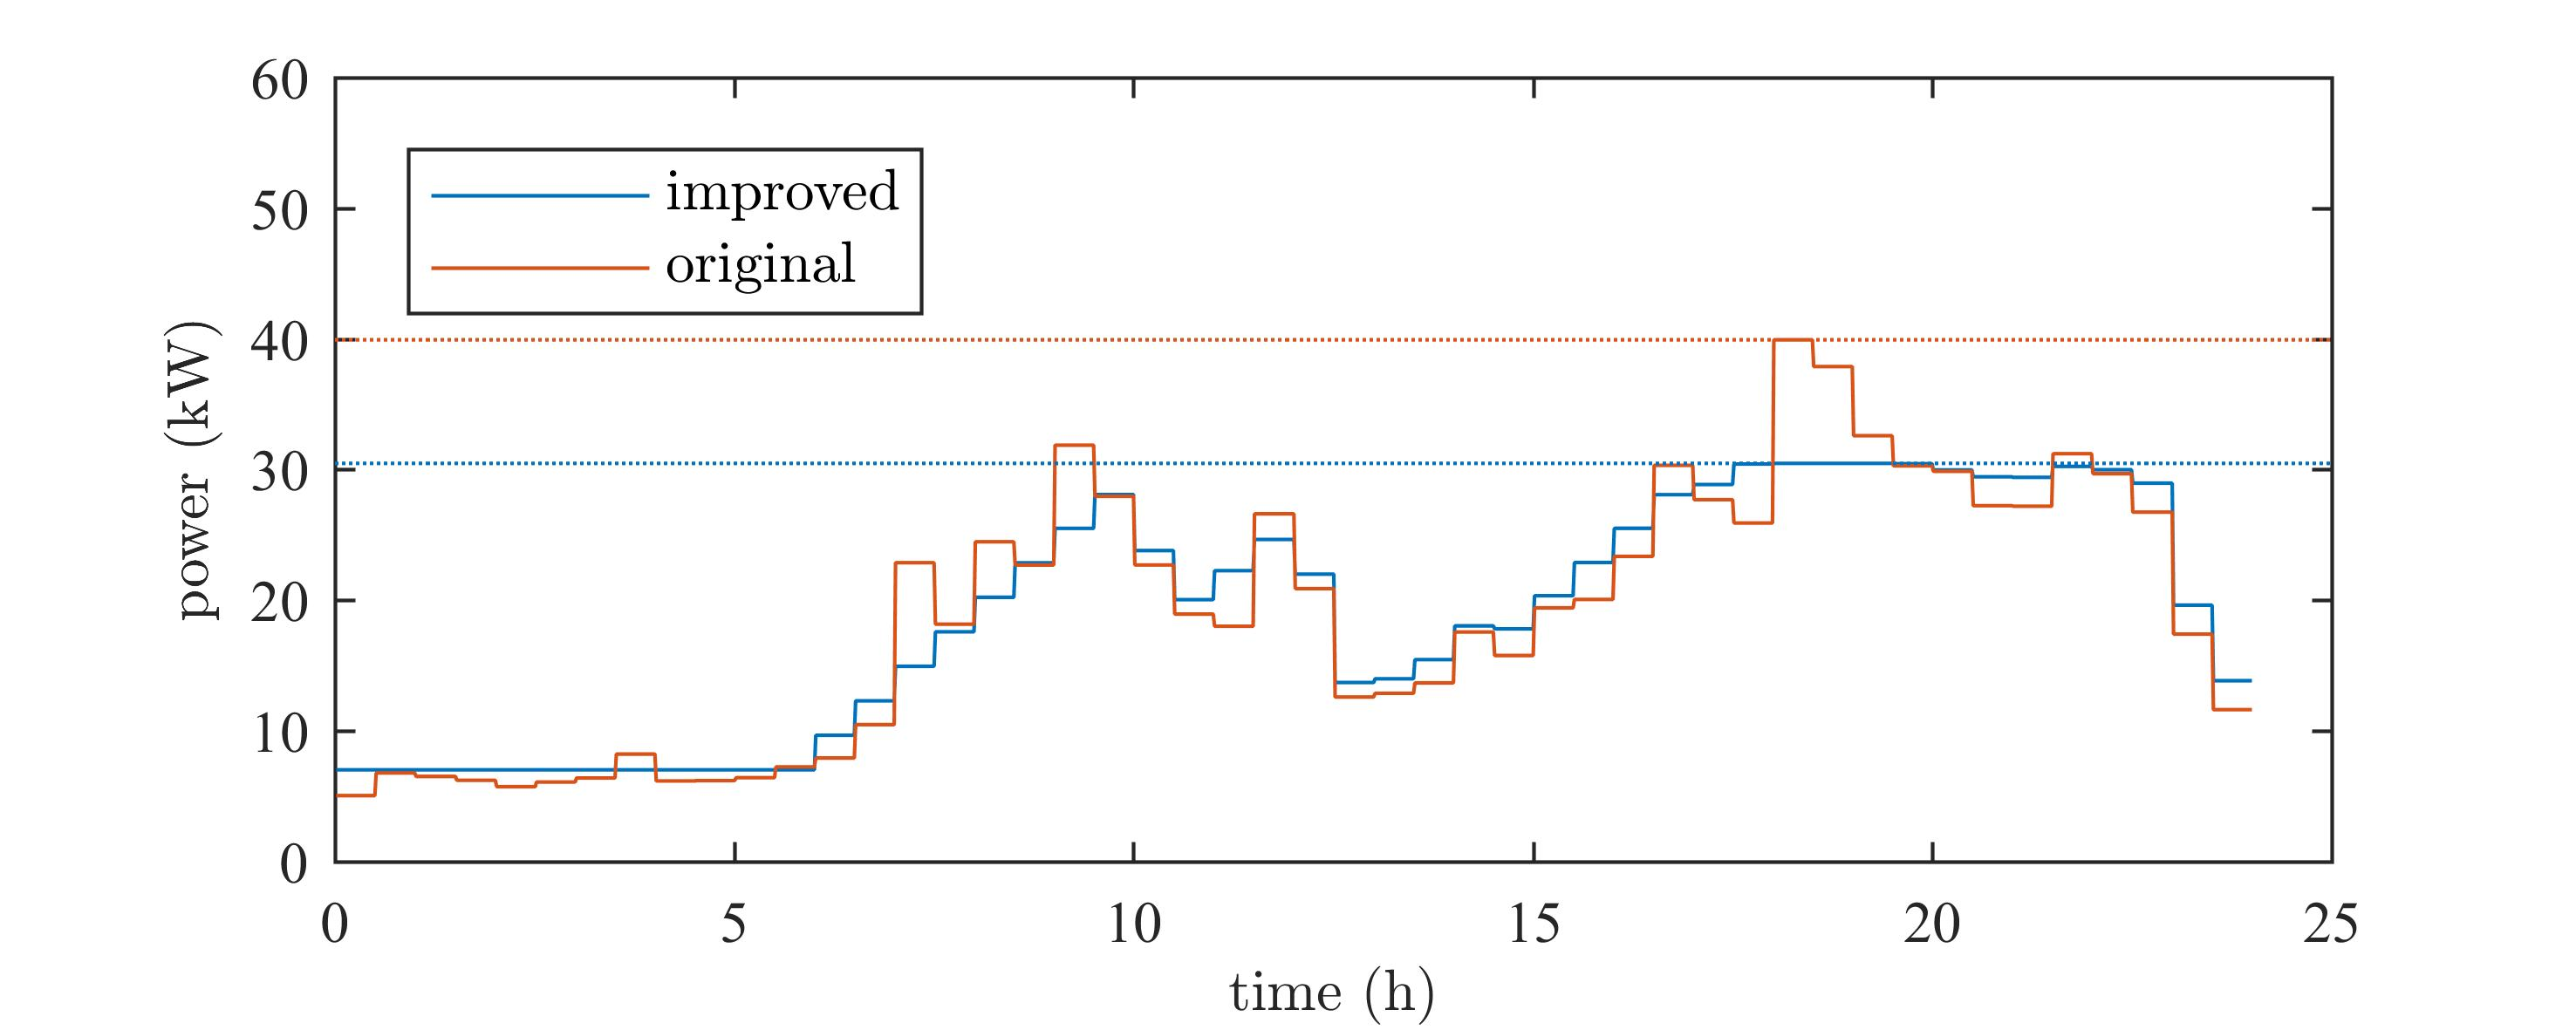
\includegraphics{_chapter1/fig/improved-half-hourly-network-power}%
		\label{ch1:subfig:improved-half-hourly-network-power}%
	}
	\vspace{5mm}
	\subfloat[Sub-half-hourly ESMU power impact ($\Delta S = 6.36kW$)]{%
		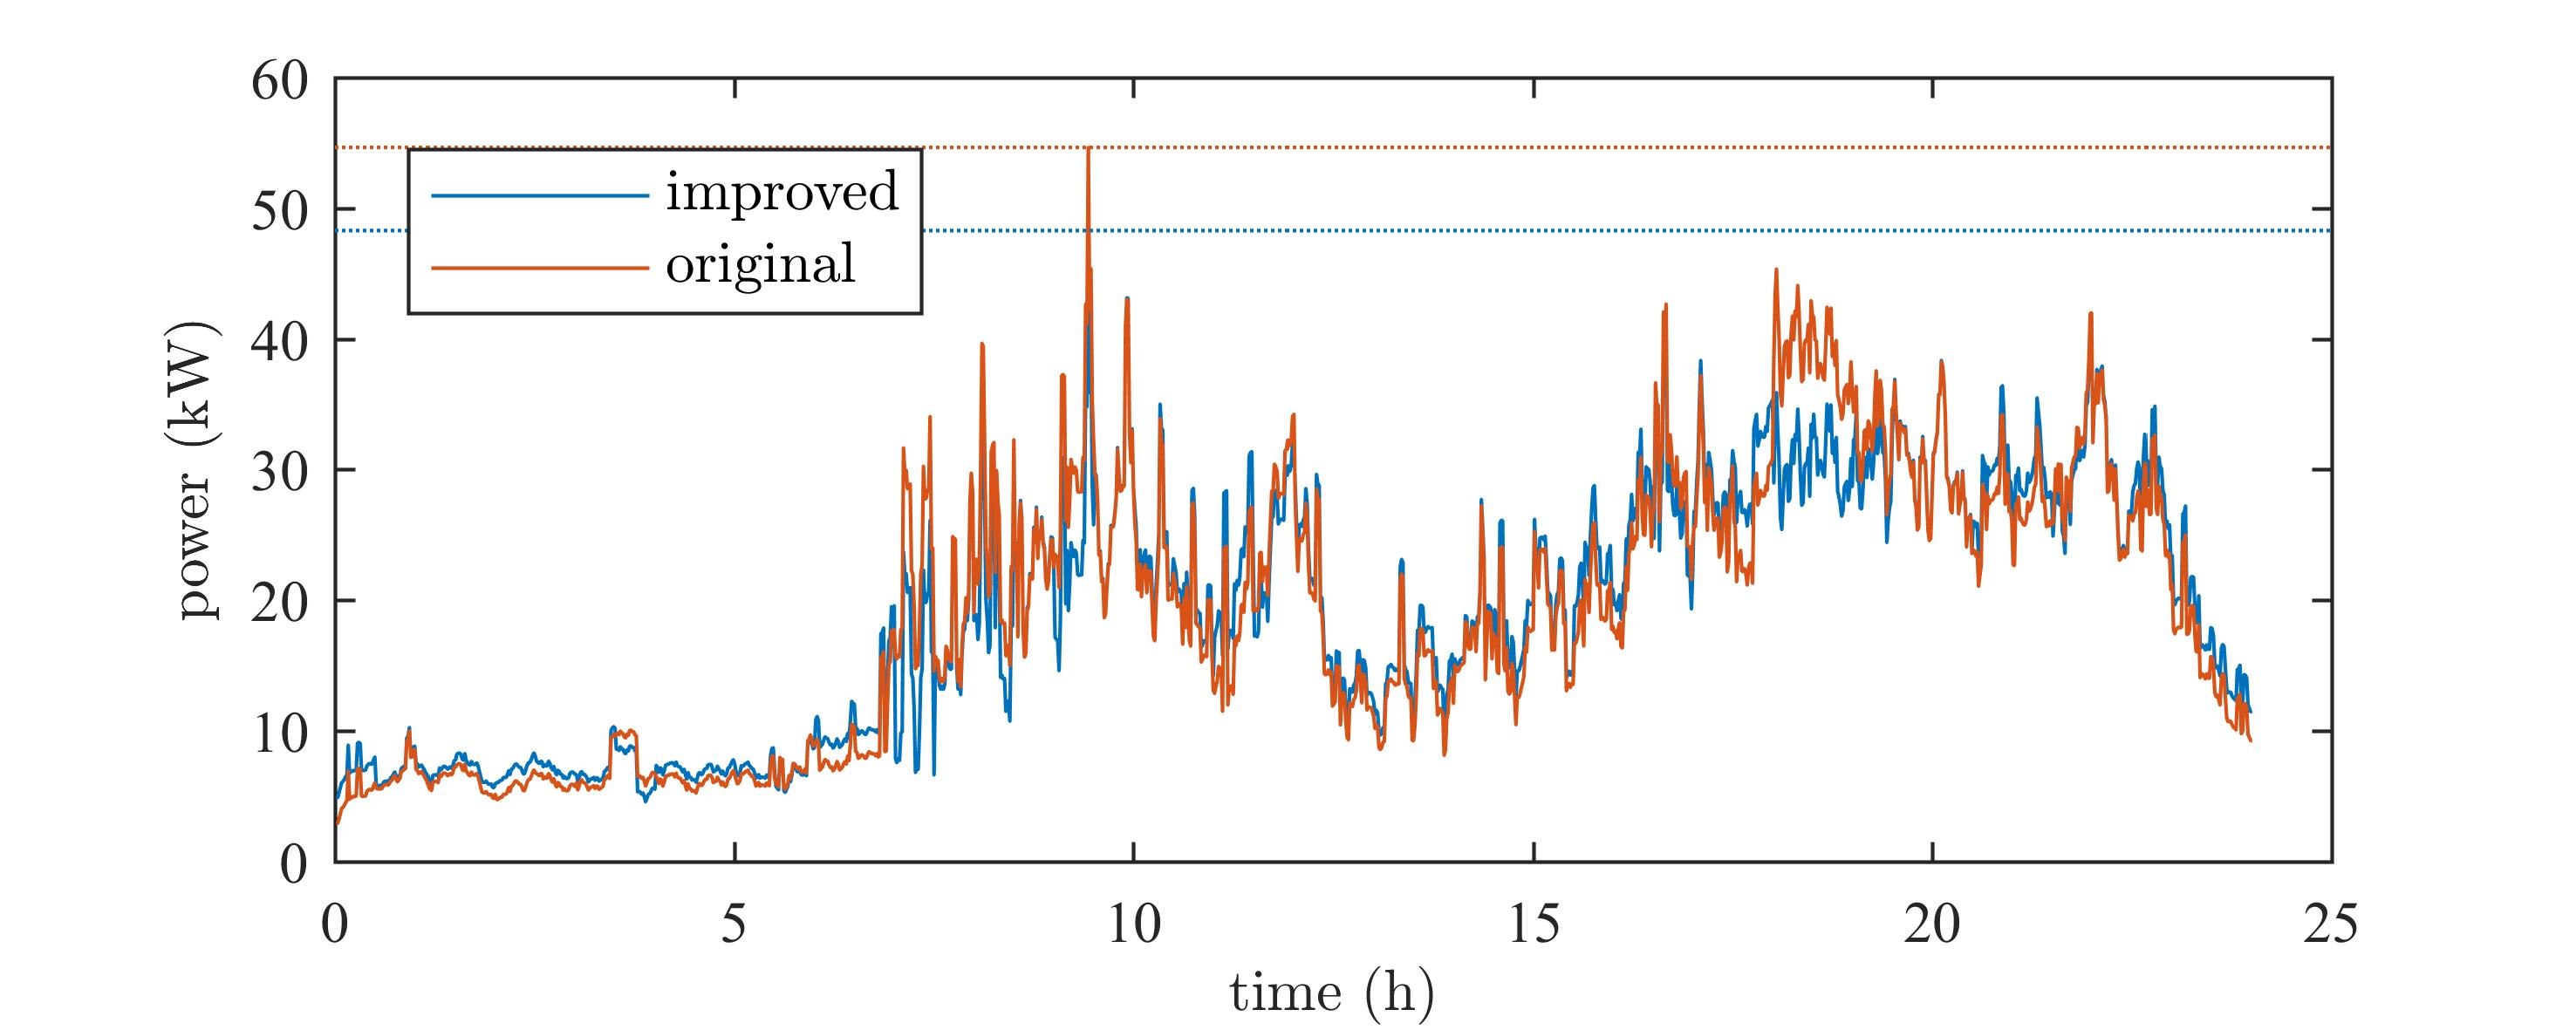
\includegraphics{_chapter1/fig/improved-sub-half-hourly-network-power}%
		\label{ch1:subfig:improved-sub-half-hourly-network-power}%
	}
	\caption{Impact of half-hourly ESMU schedule on sub-half-hourly power profile}
	\label{ch1:fig:improved-network-power}
\end{figure}

Figure \ref{ch1:fig:improved-network-power} shows the original half-hourly network load and the improved network when adding the half-hourly ESMU schedule.
For this preliminary result, no network simulations have been carried out, as it should show an idea ESMU impact on the network's load.
This positive impact can be seen, since the half-hourly profile in Figure \ref{ch1:subfig:improved-half-hourly-network-power} is dominated by an evening peak in demand.
However, the actual sub-half-hourly demand, as it is plotted in Figure \ref{ch1:subfig:improved-sub-half-hourly-network-power}, has a much larger demand spike during the morning hours, which is not addressed as strongly as the evening peak.
Therefore, the compared peak power shaving dropped from 9.46kW to only 6.36kW, although only 50\% of the battery's discharge capacity is used.
Nonetheless, the overall improvement yielded by the ESMU schedule is still noticeable (given that it was scheduled using perfect half-hourly foresight). 

In the following section, the underlying closed-loop schedule adjustment method is explained, where it will be shown how individual key network parameters can be positively impacted without deviating from this already optimised half-hourly schedule.
The constraint of having to follow this half-hourly ESMU schedule is lifted in Chapter \ref{ch2}, where a real-time schedule adjustment method is proposed and researched.

\subsection{Closed-Loop Schedule Adjustment}

To quickly summarise, the following key network parameters are used in this chapter:

\begin{itemize}
	\item substation phase voltages, $v_{ss,\phi}(t) \in \textbf{v}_{ss}(t)$,
	\item ESMU phase voltages, $v_{\text{ESMU},\phi}(t) \in \textbf{v}_\text{ESMU}(t)$,
	\item all load voltages, $v_{load,i}(t) \in \textbf{v}_\text{load}(t)$,
	\item substation apparent phase power, $s_{ss,\phi}(t) \in \textbf{s}_{ss}(t)$,
	\item substation phase currents, $i_{ss,\phi}(t) \in \textbf{i}_{ss}(t)$,
	\item all line currents, $i_{\text{line},l,\phi}(t) \in \textbf{i}_\text{line}(t)$, and
	\item all network losses, $s_\text{losses}(t)$.
\end{itemize}

Together with these key network parameters, and the cost functions defined in Section \ref{ch1:sec:key-network-parameters}, a weighted sum of all costs is generated and formalised into the following global cost function:

\begin{multline}
	\zeta(\textbf{v}_\text{ss}(t), \textbf{v}_\text{ESMU}(t), \textbf{v}_{\text{load}}(t), \textbf{s}_{ss}(t), \textbf{i}_{ss}(t), \textbf{i}_{\text{line}}(t), s_\text{losses}(t), \boldsymbol{\alpha}) :=\\
	\alpha_1 \sum_{\phi=1}^\Phi\zeta_\text{voltage}(v_{\text{ss},\phi}(t))%\\
	+ \alpha_2 \sum_{\phi=1}^\Phi\zeta_\text{voltage}(v_{\text{ESMU},\phi}(t))%\\
	+ \alpha_3 \zeta_\text{\text{load} voltage}(\textbf{v}_{\text{load}}(t))\\
	+ \alpha_4 \zeta_\text{unbalance}(\textbf{s}_{ss}(t))%\\
	+ \alpha_5 \zeta_\text{PF}(\textbf{s}_{ss}(t))%\\
	+ \alpha_6 \zeta_{\text{neutral load}}(\textbf{s}_{ss}(t))\\
	+ \alpha_7 \zeta_\text{fuse utilisation}(\textbf{i}_{ss}(t))%\\
	+ \alpha_8 \zeta_\text{\text{line} utilisation}(\textbf{i}_{\text{line}}(t))%\\
	+ \alpha_9 \zeta_\text{losses}(s_\text{losses}(t)) \\
	 \text{where } \phi \in \{1, \dots, \Phi\} \text{ and } \Phi \in \mathbb{Z}_{>0} \text{ and } \boldsymbol{\alpha} = \{\alpha_1, \dots, \alpha_9\}
\label{ch1:equ:weighted-sum-cost-function}
\end{multline}

Here, $\boldsymbol{\alpha}$ is a binary choice vector, with which the weight of the global cost function can easily be adjusted.
In other words, this vector allows to target the network improvement based by focusing on a specific cost, rather than optimising the network operation based on the complete set of (sometimes contradicting) costs.
Since all key network parameters are outputs of the power flow simulations and not directly adjustable, and for simpler notations throughout this section, the global cost function is shortened to $\zeta(\boldsymbol{\alpha})$.

\begin{figure}\centering
% Define some block styles
\tikzstyle{title} = [%
	rectangle,%
%	minimum height=2em,%
	text centered%
]
\tikzstyle{function} = [%
	rectangle,%
	draw,%
	fill=white,%
%	minimum height=2em,%
	rounded corners=5pt,%
]

\begin{tikzpicture}[node distance=3cm, shorten >= 1pt, >=stealth', auto, anchor=west]
	
	\def\title_offset{-1.33};
	\def\image_offset{-2.66};
	
	\node at (0, 0) (closed_loop_optimisation) [title] {Closed-Loop Optimisation};

	\node at (0, \title_offset+\image_offset) (opendss_logo) [rectangle] {
\includegraphics[height=7.5mm]{_chapter1/fig/OpenDSS}};
	\node (simulation_text) [rectangle, right of=opendss_logo, xshift=-1.5cm] {Simulation};
	\node (simulation) [function, fit={(opendss_logo) (simulation_text)}] {};
	\node at (0, \title_offset+\image_offset) (opendss_logo) [rectangle] {
\includegraphics[height=7.5mm]{_chapter1/fig/OpenDSS}};
	\node (simulation_text) [rectangle, right of=opendss_logo, xshift=-1.5cm] {Simulation};
	
	\node at (0, \title_offset) (matlab_cost) [rectangle] {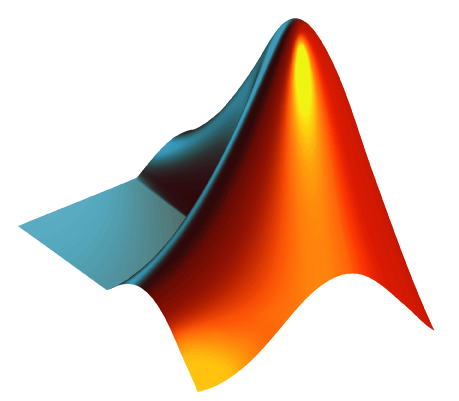
\includegraphics[height=7.5mm]{_chapter1/fig/MATLAB}};
	\node (cost_function_text) [rectangle, right of=matlab_cost, xshift=-1.15cm] {Cost Function};
	\node (cost_function) [function, fit={(matlab_cost) (cost_function_text)}] {};
	\node at (0, \title_offset) (matlab_cost) [rectangle] {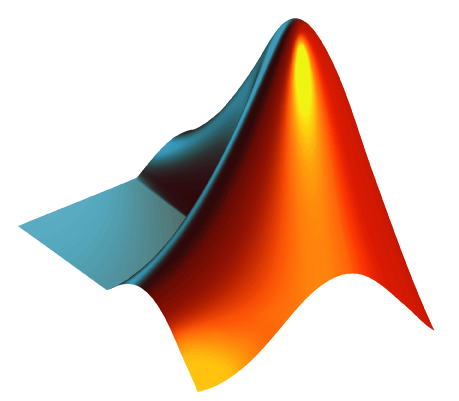
\includegraphics[height=7.5mm]{_chapter1/fig/MATLAB}};
	\node (cost_function_text) [rectangle, right of=matlab_cost, xshift=-1.15cm] {Cost Function};
	
	\node at (7, \title_offset) (matlab_optimiser) [rectangle] {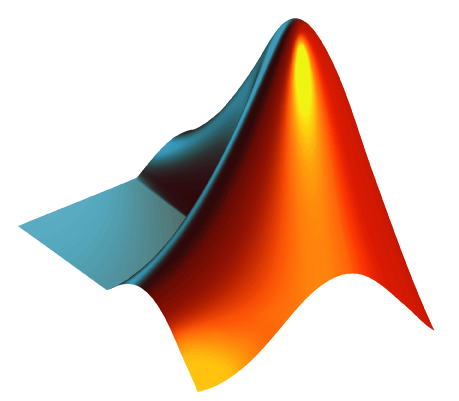
\includegraphics[height=7.5mm]{_chapter1/fig/MATLAB}};
	\node (optimiser_text) [rectangle, right of=matlab_optimiser, xshift=-1.5cm] {Optimiser};
	\node (optimiser) [function, anchor=center, fit={(matlab_optimiser) (optimiser_text)}] {};
	\node at (7, \title_offset) (matlab_optimiser) [rectangle] {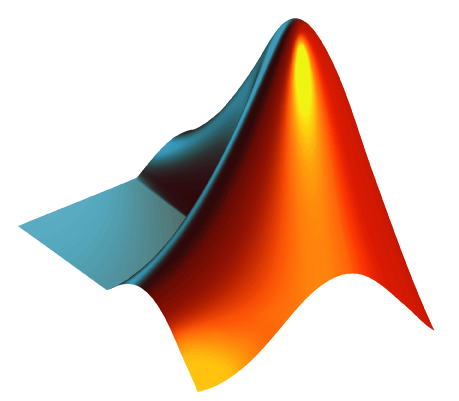
\includegraphics[height=7.5mm]{_chapter1/fig/MATLAB}};
	\node (optimiser_text) [rectangle, right of=matlab_optimiser, xshift=-1.5cm] {Optimiser};
	
	\node at (8, \title_offset+\image_offset) (addition) [state, fill=white] {$+$};
	
	\node at (12.5, \title_offset-2) (battery) [rectangle] {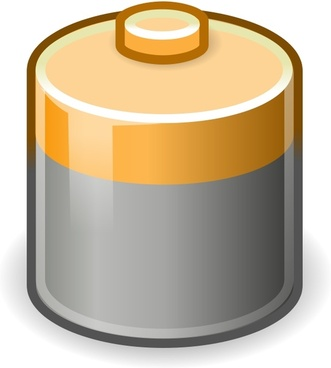
\includegraphics[height=15mm]{_chapter1/fig/battery}};
	\node (model_text) [rectangle, below of=battery, yshift=1.9cm] {Model};
	\node (model) [function, fit={(battery) (model_text)}] {};
	\node at (12.5, \title_offset-2) (battery) [rectangle] {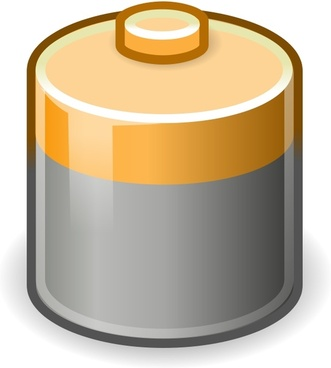
\includegraphics[height=15mm]{_chapter1/fig/battery}};
	\node (model_text) [rectangle, below of=battery, yshift=1.9cm] {Model};
	
	\node (output) [function, below of=addition, fill=yellow!20, yshift=1cm, inner sep=1em] {Output};
	
	\begin{scope}[on background layer]
		\node [draw=black, fill=green!20, fit={%
			(closed_loop_optimisation)%
			(simulation)%
			(cost_function)%
			(optimiser)}] {};
	\end{scope}

	\draw [->, bend left] (simulation) to node {key parameters} (cost_function);
	\draw [->] (cost_function) to node [above] {$\zeta(\boldsymbol{\alpha})$} (optimiser);
	\draw [->, bend left] (optimiser) to node [left] {$\delta \textbf{s}_{ESMU}(t)$} (addition);
	\draw [->] (addition) to node [above] {$\textbf{s}_{ESMU}(t) + \delta \textbf{s}_{ESMU}(t)$} (simulation);
	\draw [->] (model.west|-addition) to node [above, pos=0.3] {$\textbf{s}_{ESMU}(t)$} (addition);
	\draw [->, dashed, bend right, color=red] (model) to node [midway, above, yshift=1mm] {constraints} (optimiser.east|-optimiser.center);
	\draw [->] (addition) -- (output);
\end{tikzpicture}
\caption{ESMU schedule adjustment flow diagram}
\label{ch1:fig:closed-loop-optimisation}
\end{figure}

The underlying method that performs the proposed closed-loop optimisation is captured in the next Figure \ref{ch1:fig:closed-loop-optimisation}.
Here, for each time slot, $t$, a pre-scheduled ESMU power vector, $\textbf{s}_\text{ESMU}(t)$, is extracted and adjusted by an offset vector, $\delta \textbf{s}_\text{ESMU}(t)$.
This offset vector is found through the aforementioned optimiser that minimises the global cost function, $\zeta(\boldsymbol{\alpha})$, by repetitively running power flow simulations of the IEEE distribution feeder.
Once the adjusted ESMU schedule (i.e. $\textbf{s}_\text{ESMU}(t) + \delta \textbf{s}_\text{ESMU}(t)$) is no longer changed by the optimiser, the closed-loop optimisation process ends and the simulation continues to the next time slot (i.e. $t+1$).

Since $\delta \textbf{s}_\text{ESMU}(t)$ must not impact the underlying half-hourly ESMU schedule, one more constraint is defined.
This constraint assures that the sum of all phase powers in the adjustment vector equates to zero, hence keeping the internal battery's dis/charging power the same.
Including the previously mentioned battery system constraints, which ensure that the ESMU operates within its technical limitations (e.g. to not over- or undercharge the battery), the minimisation problem for the closed-loop optimisation mechanism can be formulated as follows:

\begin{equation}
\begin{split}
	\min_{\delta \textbf{s}_\text{ESMU}(t)} \zeta(\boldsymbol{\alpha})
	&\text{ s.t.}
	\begin{cases}
		\sum_{\phi=1}^{\Phi} \text{Re} \left(s_{\text{ESMU},\phi}(t)\right) = 0 \\
		p_\text{bat}(t) \leq C_f\times C_\text{bat} \\
		\left|s_{\text{ESMU},\phi}(t)\right| \leq S_\text{rating} \forall \phi \\
		0 \leq SOC(t) \leq 1 
	\end{cases}\\
	&\text{ where } (s_{\text{ESMU},\phi}(t)) = \textbf{s}_\text{ESMU}(t) \text{ and } \Phi \in \mathbb{Z}_{>0}
\end{split}
\label{ch1:equ:closed-loop-minimisation}
\end{equation}



\subsection{Method Execution and Result Assessment Procedure}
\label{ch1:subsec:method-execution}

After having established what parameters to focus on when trying to improve network operation, and after having established how the closed-loop optimising method aims to achieve this improvement, the performance assessment for the improvement method is introduced now.
To support the explanation of the evaluation procedure, the entire assessment procedure is captured in Figure \ref{ch1:fig:method-evaluation-flowchart}.

\begin{figure}\centering

% Define some block styles
\tikzstyle{data} = [rectangle, draw, inner sep=1em, text centered, rounded corners=5pt, fill=white]
\tikzstyle{method} = [rectangle, draw, inner sep=1em, text centered, align=center]
\tikzstyle{output} = [rectangle, draw, minimum height=1cm, minimum width=2.5cm, text centered, rounded corners=5pt, fill=yellow!20]

\scalebox{0.7}{%
\begin{tikzpicture}[node distance=3cm, shorten >= 1pt, >=stealth', auto, anchor=west]
	
	\node (centre) [] {};
	
	\node (power_profiles) [data, left of=centre, xshift=1cm] {Power Profiles};
	\node (battery_model) [data, right of=centre, xshift=-1cm] {Battery Model};
	
	\node (inputA) [left of=battery_model, yshift=1cm, xshift=-9cm] {};
	\node (inputB) [left of=battery_model, yshift=-1cm, xshift=-9cm] {};
	\draw [decorate,decoration={brace,mirror,amplitude=10pt,raise=4pt},yshift=0pt] (inputA) -- (inputB) node [left,black,midway,align=center,xshift=-10mm,rotate=90,anchor=center] {Input Data};
	
	\node (optimisation) [method, below right of=battery_model, yshift=-1.5cm, fill=green!20] {Closed-Loop Optimisation Method};
	\node (normal_run) [method, left of=optimisation, xshift=-3.5cm, fill=blue!20] {Normal Simulation};
	\node (base_run) [method, left of=normal_run, xshift=-1.5cm, fill=red!20] {Base Simulation};
	
	\node (simA) [left of=battery_model, yshift=-2.2cm, xshift=-9cm] {};
	\node (simB) [left of=battery_model, yshift=-5.2cm, xshift=-9cm] {};
	\draw [decorate,decoration={brace,mirror,amplitude=10pt,raise=4pt},yshift=0pt] (simA) -- (simB) node [left,black,midway,align=center,xshift=-10mm,rotate=90,anchor=center] {Simulations};
	
	\draw [->, out=270, in=120] (power_profiles.south) to (optimisation.north);
	\draw [->, out=270, in=90] (power_profiles.south) to (normal_run.north);
	\draw [->, out=270, in=60] (power_profiles.south) to (base_run.north);
	\draw [->, out=270, in=120] (battery_model.south) to (optimisation.north);
	\draw [->, out=270, in=60] (battery_model.south) to (normal_run.north);

	\def\offsetx{-5};
	\def\offsety{-4};
	\node (alpha_base) [output, below of=centre, yshift=\offsety cm, xshift=\offsetx cm-3cm, fill=red!20] {$base$};
	\draw [->, out=270, in=60] (base_run) to (alpha_base);
	\foreach \i [evaluate=\i as \x using 3*\i/2+\offsetx] in {0,2,...,8}
	{
		\foreach \j [evaluate=\j as \y using -1.5*\j] in {0, 1}
		{
			\pgfmathtruncatemacro{\k}{\i+1-\j}
			\if\k0
				\node (alpha_normal) [output, below of=centre, yshift=\offsety cm+\y cm, xshift=\y cm+\x cm, fill=blue!20] {$normal$};
				\begin{scope}[on background layer]\draw [->, out=270, in=60] (normal_run) to (alpha_normal);\end{scope}
			\else
				\node (alpha_\k) [output, below of=centre, yshift=\offsety cm+\y cm, xshift=\y cm+\x cm] {$\zeta(\alpha_{\k} = 1)$};
				\begin{scope}[on background layer]
					\ifnum7>\k
						\draw [->, out=270, in=60] (optimisation) to (alpha_\k);
					\else
						\ifnum7=\k
							\draw [->, out=270, in=90] (optimisation) to (alpha_\k);
						\else
							\draw [->, out=270, in=120] (optimisation) to (alpha_\k);
						\fi
					\fi
				\end{scope}
			\fi
		}
	}
	
	
	\node (dataA) [left of=battery_model, yshift=-6cm, xshift=-9cm] {};
	\node (dataB) [left of=battery_model, yshift=-9.4cm, xshift=-9cm] {};
	\draw [decorate,decoration={brace,mirror,amplitude=10pt,raise=4pt},yshift=0pt] (dataA) -- (dataB) node [left,black,midway,align=center,xshift=-10mm,rotate=90,anchor=center] {Results or\\Datasets};
	
	\foreach \i [evaluate=\i as \k using int(round(\i-1))] in {0,1,2,...,10}
	{
		\pgfmathsetmacro\x{1.5*\i}
		\pgfmathsetmacro\y{-\i*0.5};
		
		\ifnum1>\k
			\ifnum0=\i
				\node (assess_base) [method, below of=alpha_base, yshift=\y cm, xshift=\x cm, anchor=north, fill=red!20] {$base$ assessment};
				\draw [->] (alpha_base) to (assess_base);
			\else
				\node (assess_normal) [method, below of=alpha_base, yshift=\y cm, xshift=\x cm, anchor=north, fill=blue!20] {$normal$ assessment};
				\draw [->] (alpha_normal) to (assess_normal);
			\fi
		\else
			\node (assess_\k) [method, below of=alpha_base, yshift=\y cm, xshift=\x cm, anchor=north, fill=yellow!20] {$\zeta(\alpha_{\k}=1)$ assessment};
			\draw [->] (alpha_\k) to (assess_\k);
		\fi
	}


	\node (braceA) [below of=assess_base, yshift=1.5cm, xshift=-1.5cm] {};
	\node (braceB) [left of=assess_9, yshift=-1.5cm, xshift=1.5cm] {};
	\draw [decorate,decoration={brace,mirror,amplitude=10pt,raise=4pt},yshift=0pt] (braceA) -- (braceB) node [below,black,midway,yshift=-8mm,anchor={north east},align=right] {Data Assessments\\\footnotesize Each assessment is comparing \\\footnotesize all nine cost-functions};
	
\end{tikzpicture}%
}
\caption{Method execution and results assessment flowchart}
\label{ch1:fig:method-evaluation-flowchart}
\end{figure}

All in all, there are eleven datasets of simulation results to be assessed and compared.
These results are obtained from a \textit{base} simulation, a \textit{normal} simulation and nine additional simulations where individual cost-functions were minimised.
More specifically, the \textit{base} case is the outcome of running an entire day of power profiles without any ESMU intervention.
This case represents the baseline or network performance which should be improved by any ESMU intervention.
The \textbf{normal} case captures the simplest of all ESMU interventions, since for this case, the ESMU executes its normal half-hourly schedule without any additional schedule modification.
Comparing the \textit{base} and \textit{normal} cases dies show the direct impact of the ESMU on the network's operation.
As mentioned above, the remaining nine datasets are results of nine different cases where the ESMU schedule is adjusted on a sub-half-hourly level.
The adjustment for each case is designed to minimise one underlying cost-function, whilst conforming to the ESMU's overall half-hourly charging and discharging profile.
In order to treat each cost-function separately $\boldsymbol{\alpha}$ is set to focus on each cost independently, e.g. by setting $\alpha_1 = 1 \text{ and } \alpha_2 = \alpha_3 = \dots = \alpha_9 = 0$.
For simplicity, the flowchart in Figure \ref{ch1:fig:method-evaluation-flowchart} abbreviates the specific costs by only indicating which entry in the $\boldsymbol{\alpha}$ vector is set to $1$, e.g. $\zeta(\alpha_1=1)$ for the preceding example.

All eleven datasets are then assessed in the same manner in order to compare the impact they had had on the network performance.
This underlying assessment is broken into three parts for each dataset:

\begin{enumerate}
	\item \textbf{Time Series Analysis} - 
	The underlying raw profiles are plotted and compared against their respective counterpart cases, in order to link the immediate network impacts to their physical meaning.
	For the same profiles, their corresponding cost profiles are calculated plotted.
	This is done to to highlight how the profiles are interpreted by the cost-functions in terms of improvement (i.e. lower cost) or worsening (i.e. increased cost).
	\item \textbf{Difference Analysis} - 
	The difference in cost profiles, compared to the respective \textit{base} or \textit{normal} case, is calculated and boxplots of these differences are presented to show a statistical spread of improvements or worsening.
	For these plots, a generally positive boxplot skew indicates a general improvement of the underlying network parameters, whilst a generally negative skew does indicate worse performance in regards to the underlying network parameters.
	\item \textbf{Probability Density Analysis} - 
	A set of Probability Density Functions (PDF) is derived for each cost profile using the well established kernel density estimation.
	These PDFs indicate the probability that a certain cost value occurs.
	An improvement is noted when the PDF is shifted towards the lower cost values, whereas a shift towards higher cost values worsened the network performance.
\end{enumerate}







\section{Results and Discussion}
\label{ch1:sec:results-and-discussion}

In this section, all results are presented and briefly discussed.
Each of the three assessments in this section focuses on improvements in voltage level, improvements in network efficiency (i.e. power quality and network losses), and improvements in resource utilisation.
Hence, only a subset of all results is included, but the complete set of results has been appended to this Thesis in Appendix \ref{appx-a:ch1}.

\subsection{Time Series Analysis}
\label{ch1:subsec:time-series-analysis}

The ESMU's largest impact on network voltage levels can be noticed at the ESMU's PCC.
Consequently, any adjustments to the ESMU powers should become most noticeable, too.
This impact can clearly be observed in Figure \ref{ch1:fig:ts-esmu-voltages}.

\begin{figure}\centering
	\subfloat[Voltage levels at ESMU's PCC when minimising its voltage deviation \hl{(nominal substation voltage is 252V)}]{%
		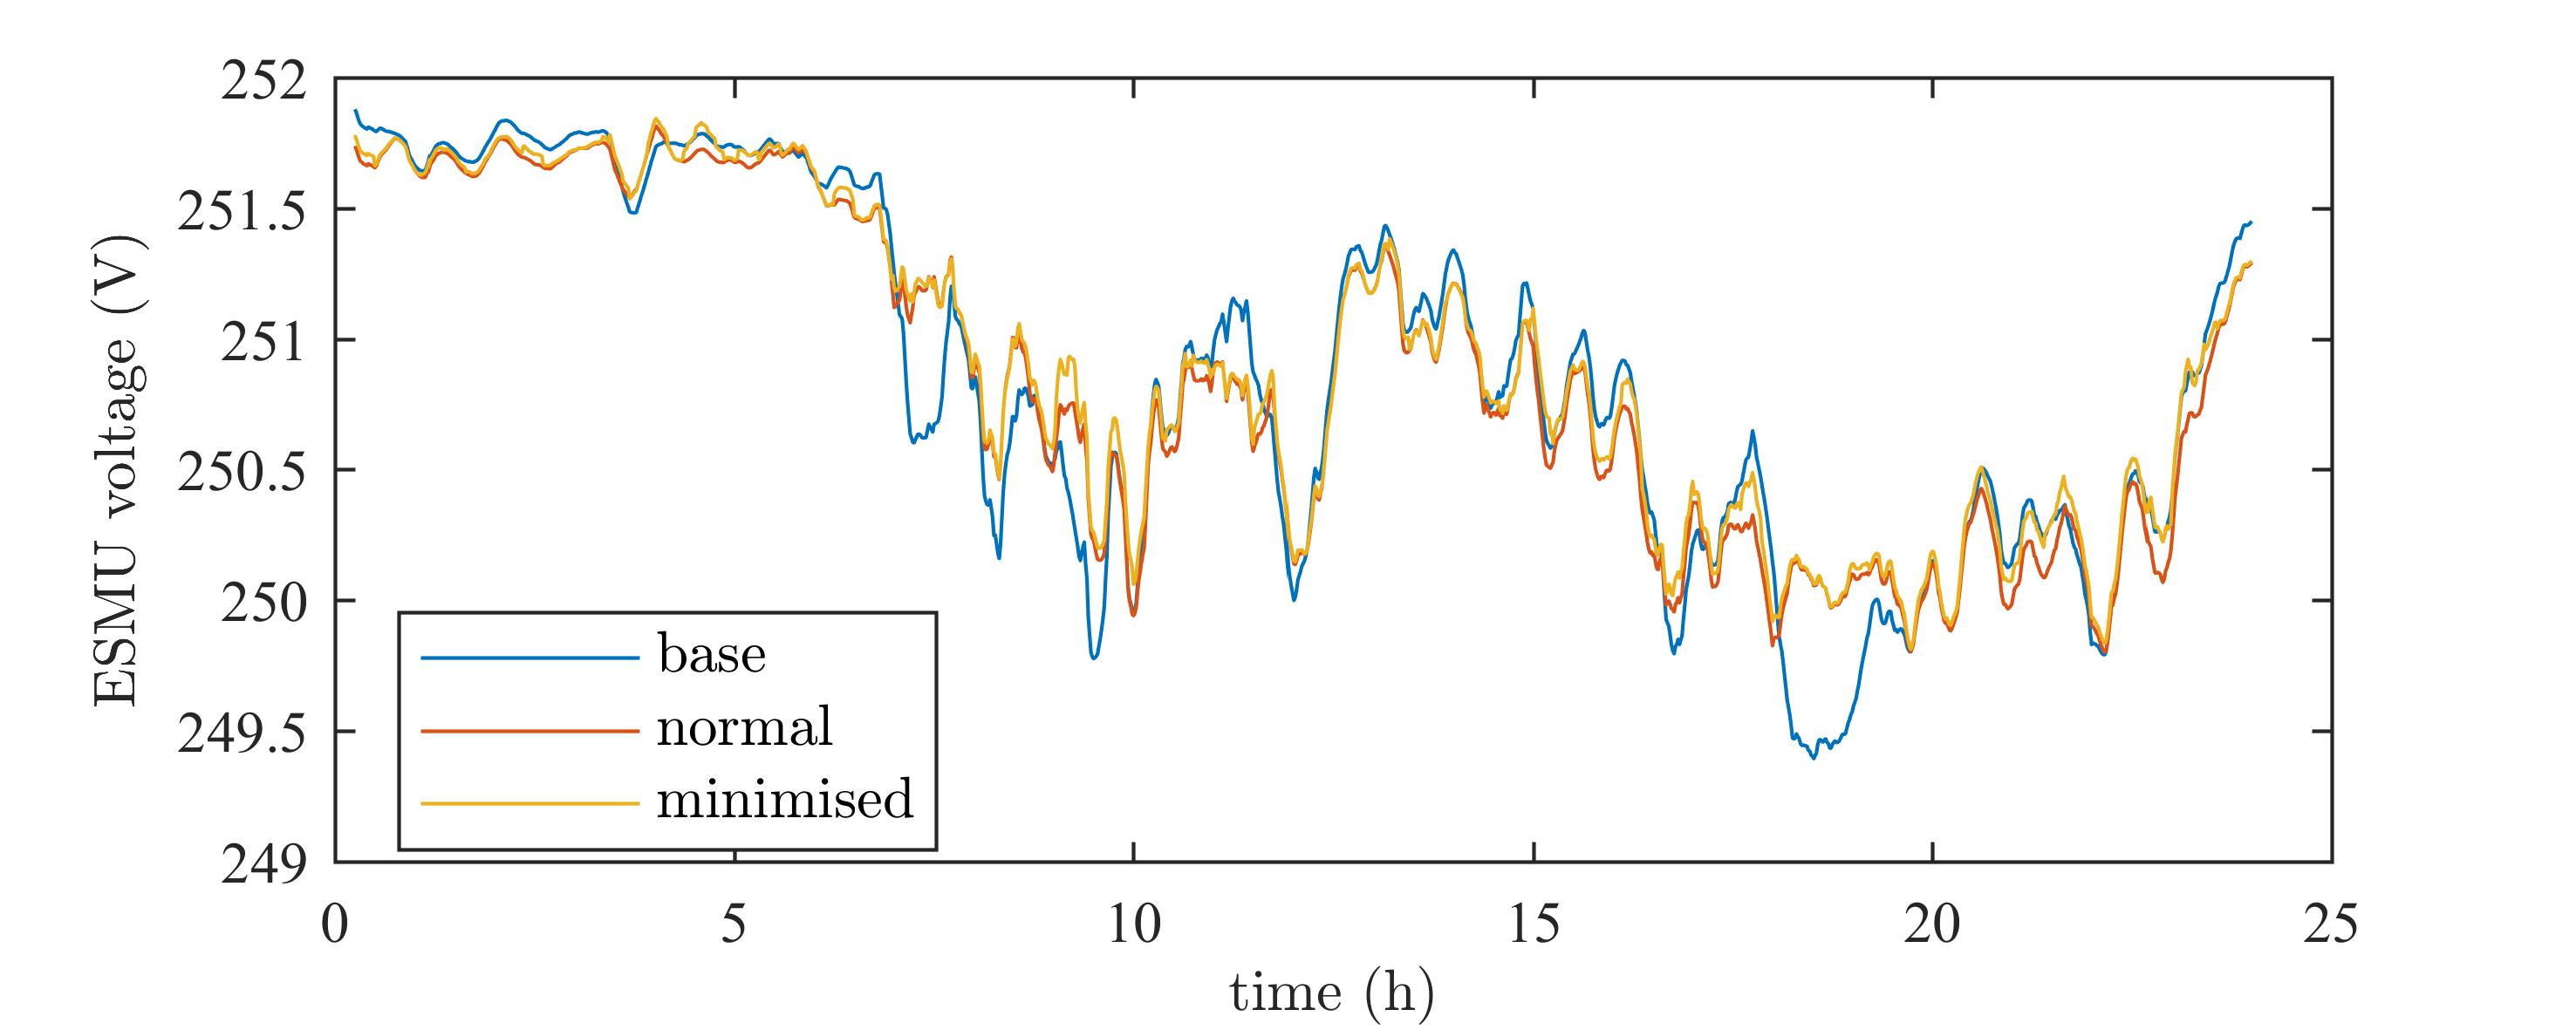
\includegraphics{_chapter1/fig/results/ts-esmu-voltages_}%
		\label{ch1:subfig:ts-esmu-voltage}%
	}\\
%	\vspace{5mm}
	\subfloat[Cost associated with the minimisation of the ESMU's PCC voltage deviation]{%
		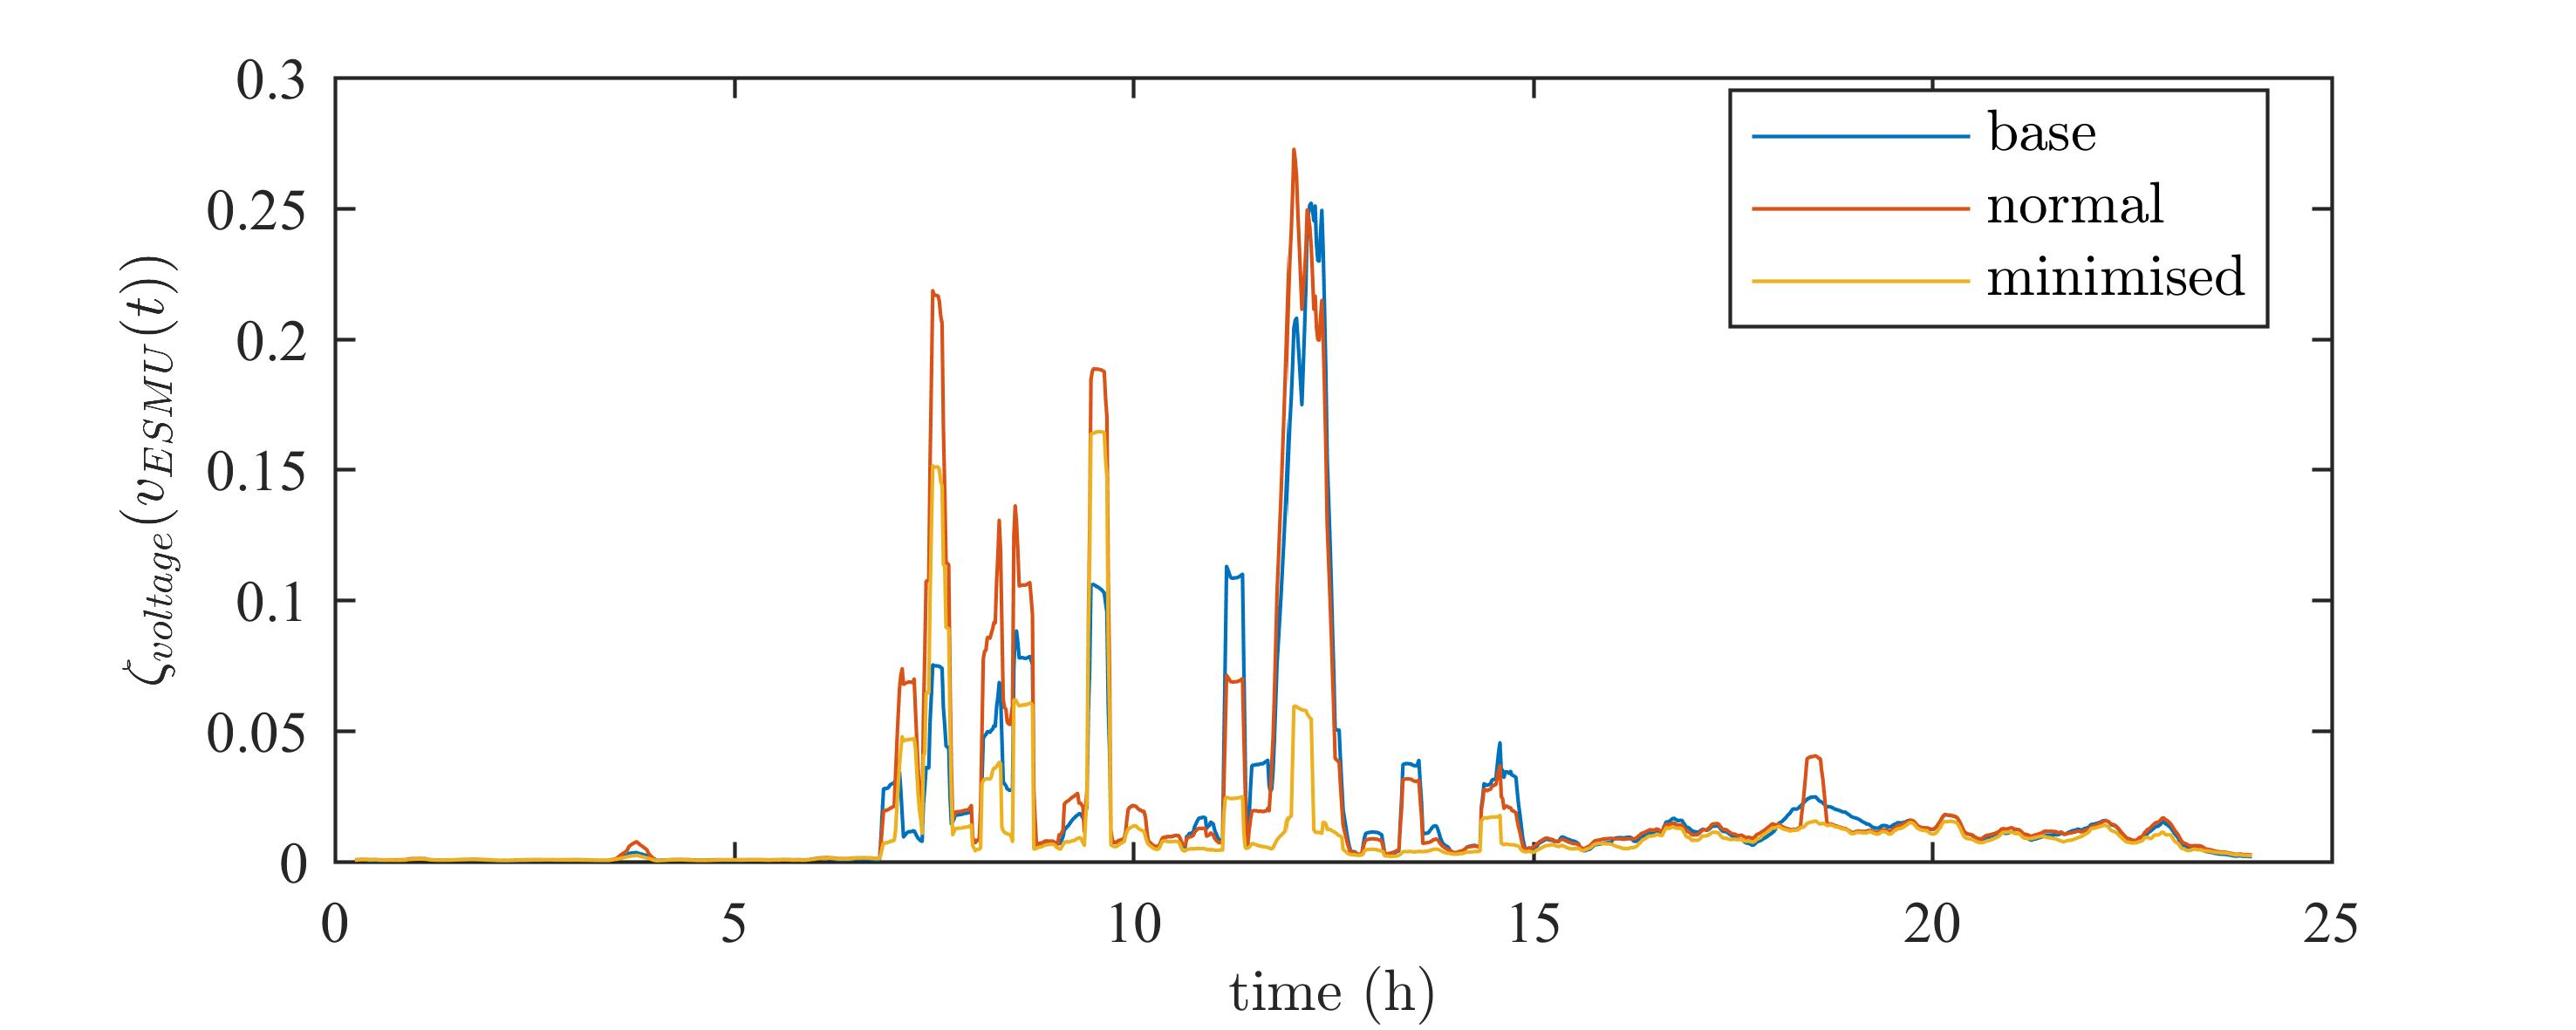
\includegraphics{_chapter1/fig/results/ts-esmu-voltages}%
		\label{ch1:subfig:ts-esmu-voltage-cost}%
	}
\caption{Voltage level modifications as noted at the ESMU's PCC by adjusting its schedule}
\label{ch1:fig:ts-esmu-voltages}
\end{figure}

In this figure, the \textit{base} and \textit{normal} case's voltage profiles are plotted alongside the \textit{minimisation} case, for which voltage deviation is minimised.
The plot shows that during the night's light load (i.e. from 0:00 to 6:00), ESMU was able to boost its voltage towards the nominal feeder voltage.
This is also the case during the lighter load in the afternoon (i.e. between 12:00-14:00).
But during the rest of the day when network load increases, the ESMU is unable to reduce voltage deviation to match its PCC voltage with the network's nominal substation voltage.
The reason behind this behaviour that the ESMU has allocated its resources to serve for the underlying half-hourly ESMU schedule.
Therefore, the remaining resources that could provide voltage support during periods of low demand become limited during periods of high demand.
Combined with the fact that the LV distribution network is more resistive than inductive (i.e. unlike HV transmission networks), reactive power injection to support voltage levels has a reduced impact.
Nonetheless, due to the constant yet small availability of power resources, the ESMU was able to boost voltages by to some extent at all times; this can be seen in Figure \ref{ch1:subfig:ts-esmu-voltage-cost}, where the associated cost has always been reduced in comparison to the base and normal.

The ability to support voltage levels at the ESMU's PCC is interesting, yet to support voltage levels at all buses throughout the network is more relevant, since some of these buses are linked to customers, for which maintaining a constant voltage level is essential.
Therefore, the next voltage plot inspects both the highest and lowest voltage level that was recorded throughout the network.

\begin{figure}\centering
	\subfloat[Highest and lowest voltage levels that were recorded throughout the network when minimising the worst voltage deviation \hl{(nominal substation voltage is 252V)}]{%
		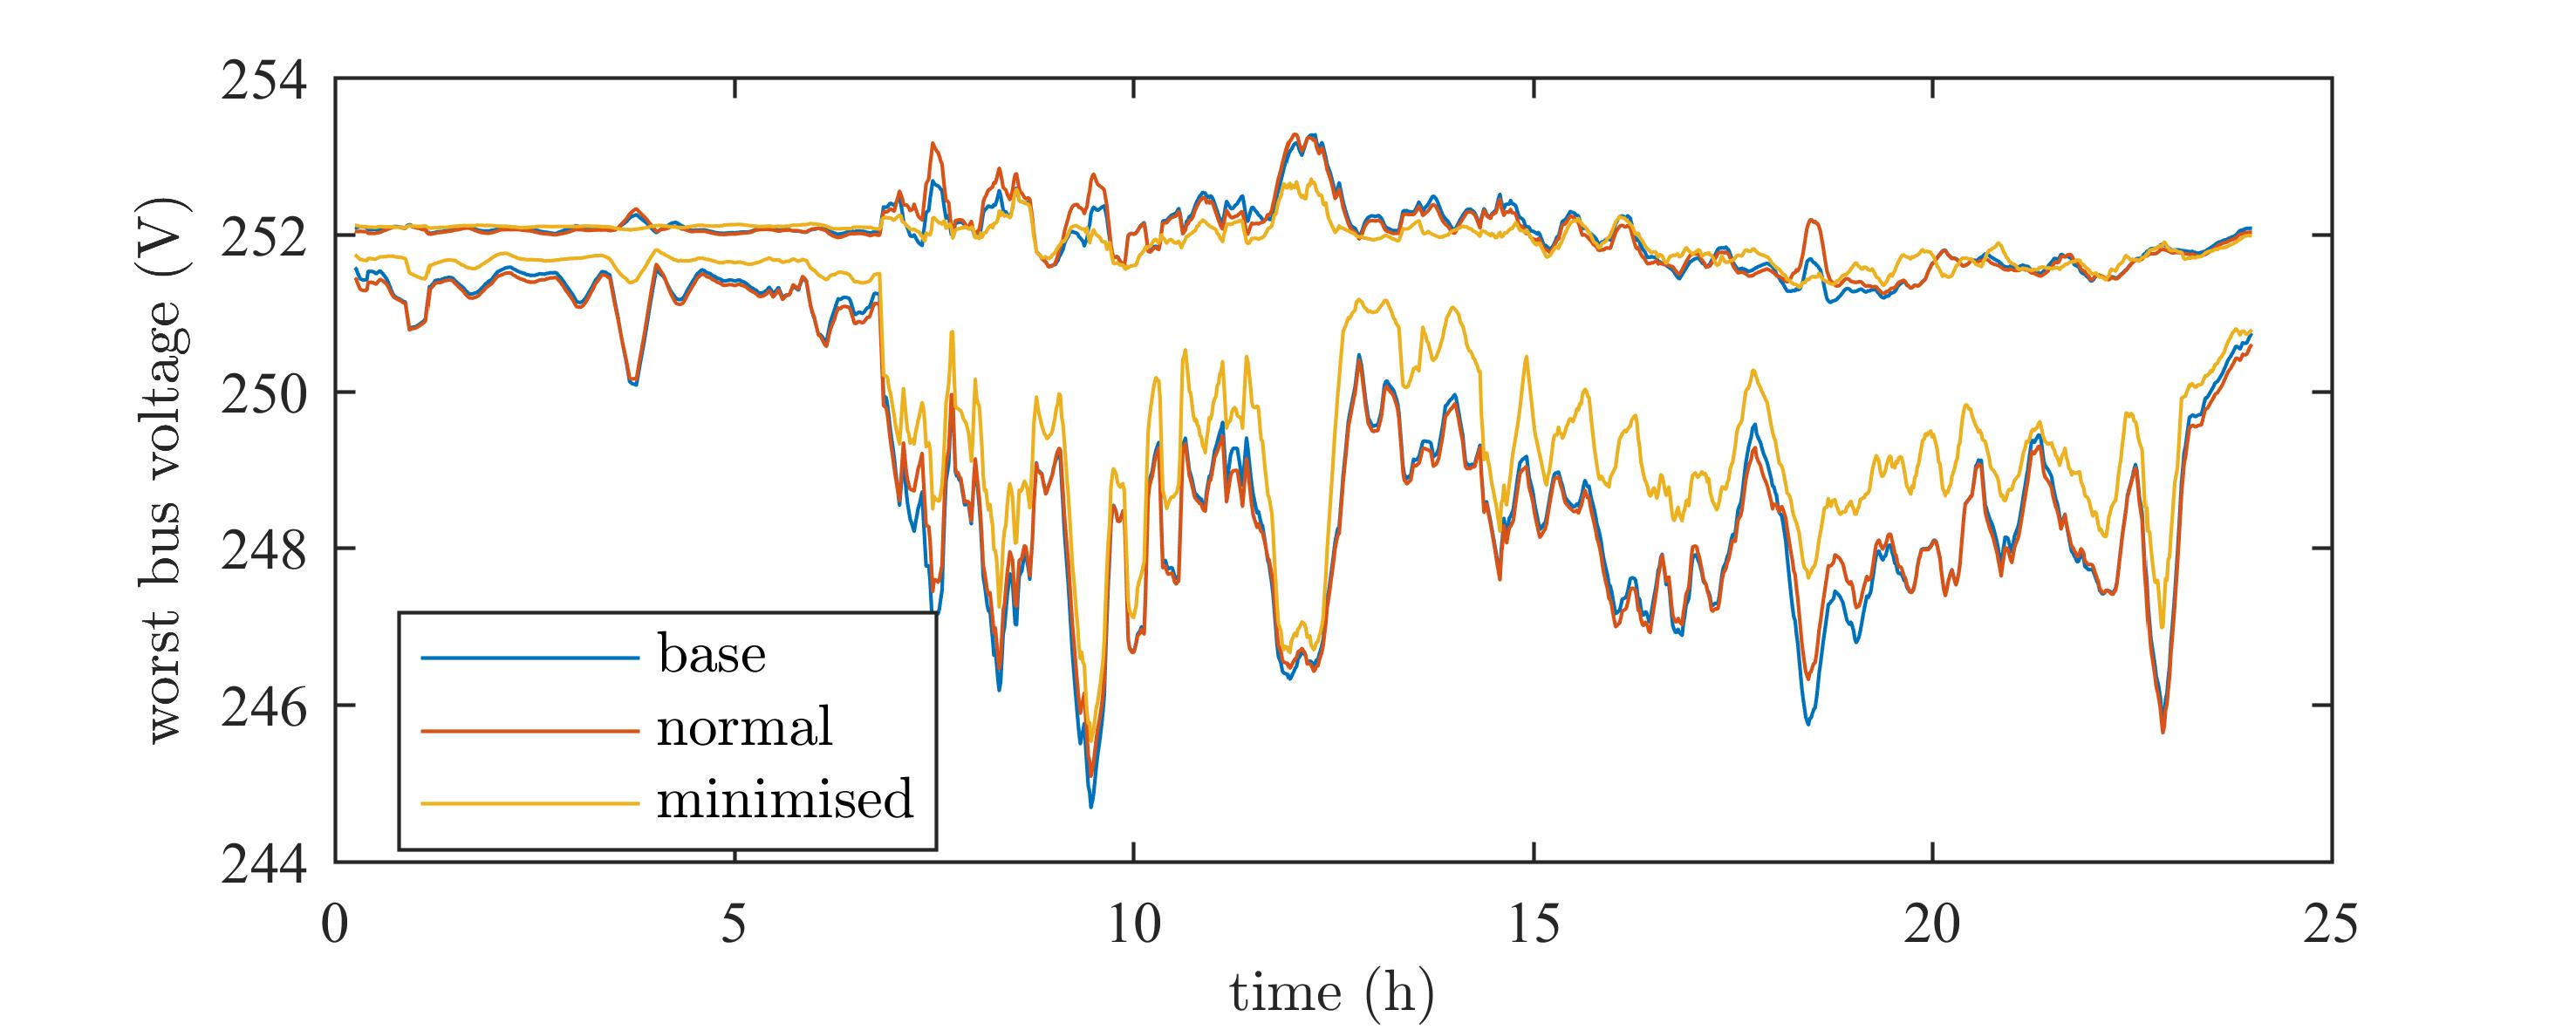
\includegraphics{_chapter1/fig/results/ts-all-voltages_}%
		\label{ch1:subfig:ts-all-voltages}%
	}\\
%	\vspace{5mm}
	\subfloat[Cost associated with the worst voltage deviation throughout the entire network]{%
		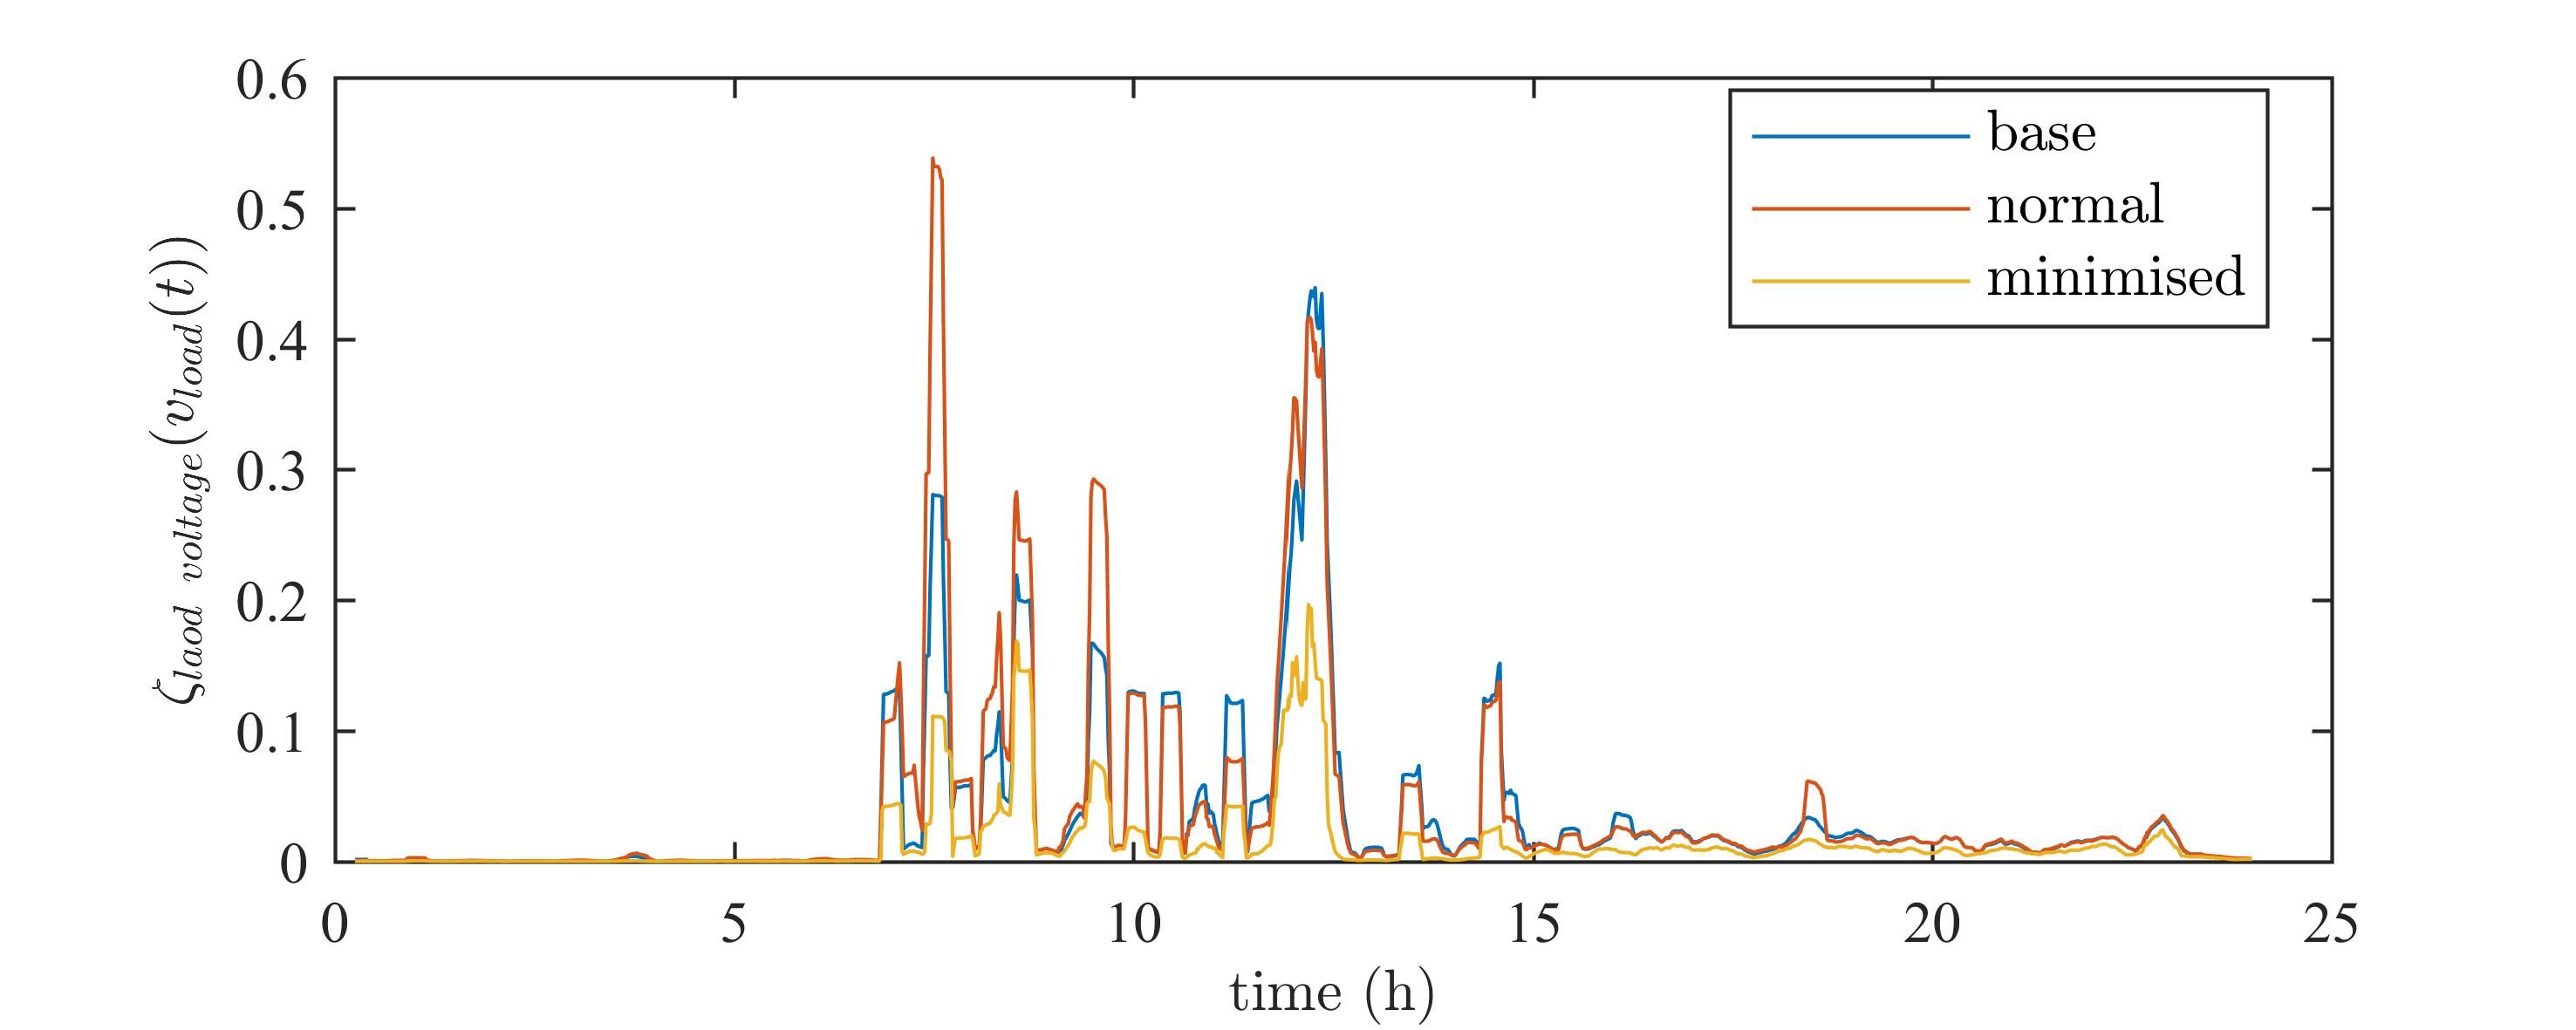
\includegraphics{_chapter1/fig/results/ts-all-voltages}%
		\label{ch1:subfig:ts-all-voltages-cost}%
	}
\caption{Voltage level improvements at all buses in the entire distribution network due to the ESMU schedule adjustment.}
\label{ch1:fig:ts-all-voltages}
\end{figure}

In Figure \ref{ch1:subfig:ts-all-voltages}, despite no voltage violations taking place due to the already boosted substation voltage, the ESMU's positive impact can be observed.
Here, the difference between highest and lowest voltage in the network was noticeably reduced at all times and their average was brought closer to the network's nominal voltage.
The ESMU's function to support the network in providing more stable voltage levels at customer endpoints can therefore be fulfilled.
This fact is also reflected in the associated cost plot, i.e. in Figure \ref{ch1:subfig:ts-all-voltages-cost}.

Beside providing stable voltage levels, power quality should also be upheld to assure that the distribution network operates as efficient as possible.
The first power related parameter that to indicate network efficiency is the phase unbalance.

\begin{figure}\centering
	\subfloat[Network's highest and lowest phase power demand when phase unbalance was minimised]{%
		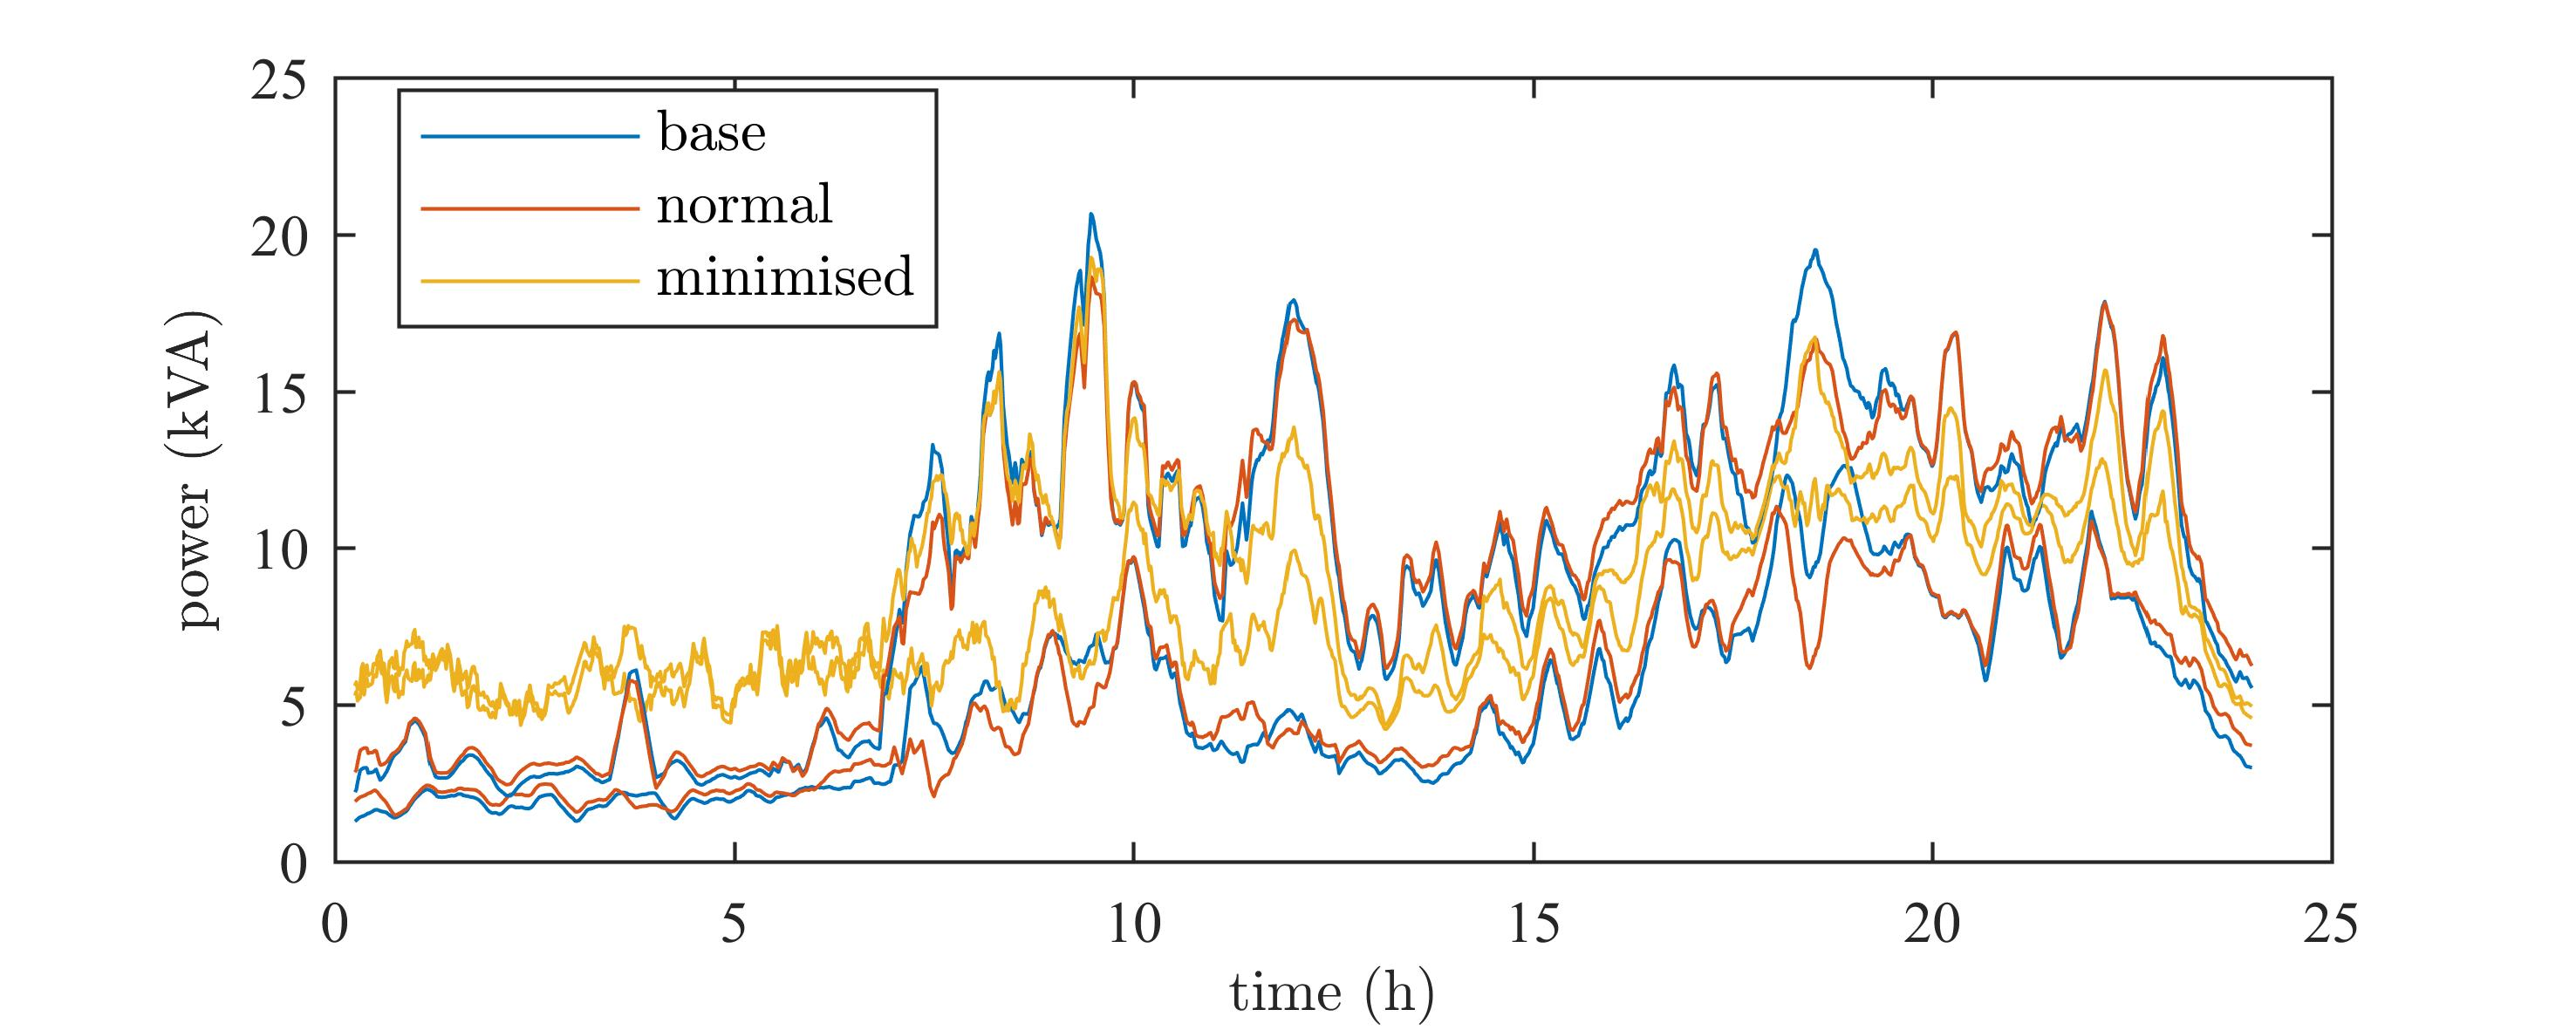
\includegraphics{_chapter1/fig/results/ts-phase-unbalance_}%
		\label{ch1:subfig:ts-phase-unbalance}%
	}\\
%	\vspace{5mm}
	\subfloat[Cost associated with the network's phase unbalance]{%
		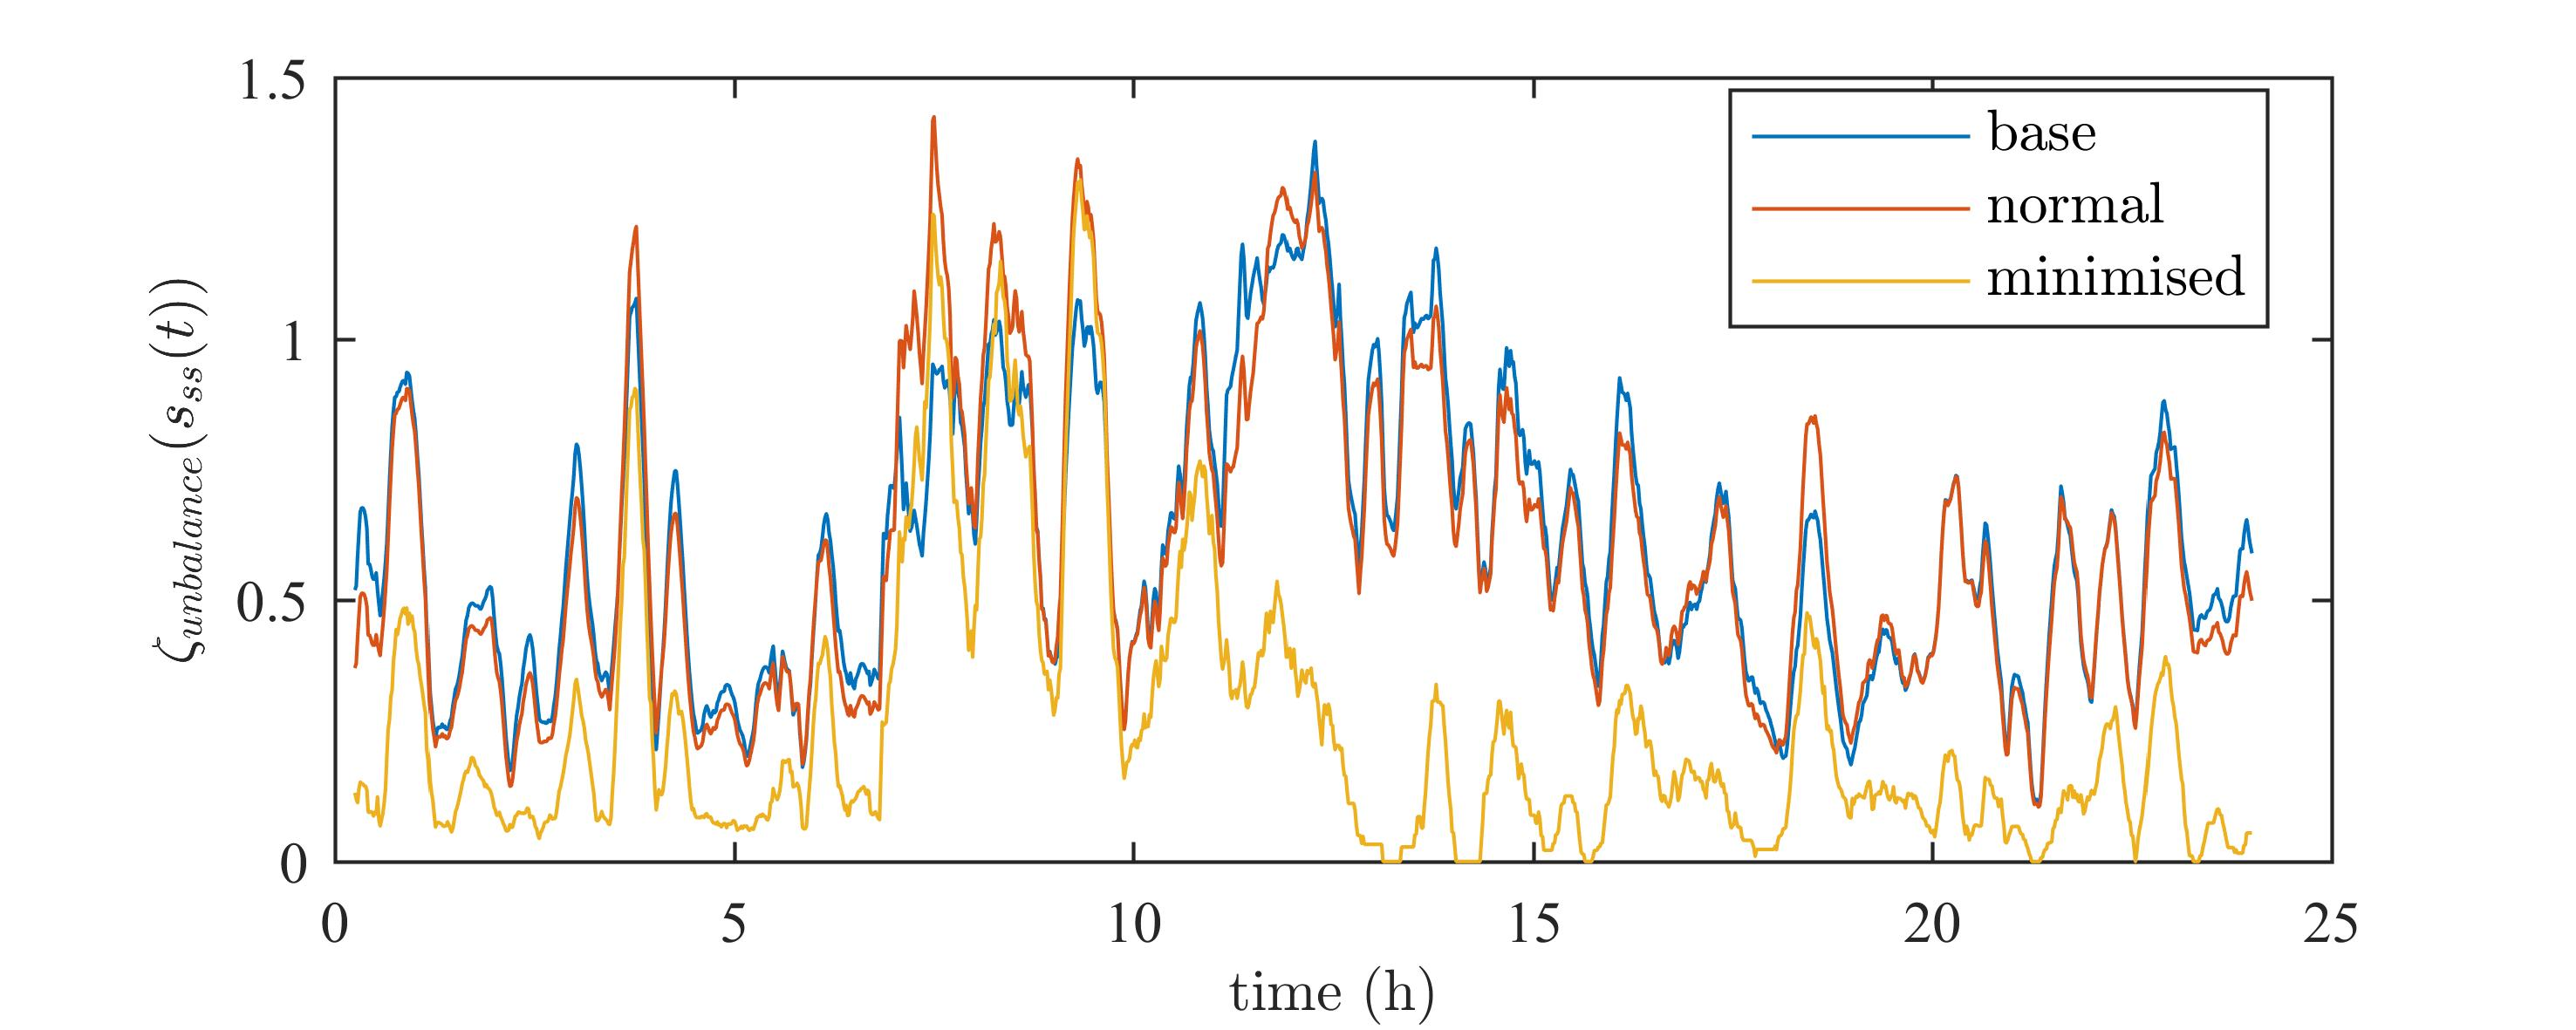
\includegraphics{_chapter1/fig/results/ts-phase-unbalance}%
		\label{ch1:subfig:ts-phase-unbalance-cost}%
	}
\caption{Reduction of the network's phase unbalance due to the adjustment of the ESMU schedule.}
\label{ch1:fig:ts-phase-unbalance}
\end{figure}

In Figure \ref{ch1:subfig:ts-phase-unbalance}, the most and least loaded phases' power values are plotted against time.
At all times, the sub-half-hourly adjustments of the ESMU's schedule could reduce the underlying phase imbalance.
It did so by alleviate some load from the most loaded phase and utilise the unused capacity on the lighter loaded phases.
Correspondingly, the associated phase unbalance cost has noticeably lowered in comparison to the normal and base cases.
It should however be noted, that phase balancing behaviour during the morning hours is predominantly comprised of reactive power injection and absorption, since the ESMU's half-hourly.
Therefore, the tradeoff between adding additional strain on the network, versus balancing phases has to be taken into account.
One unnecessary strain on the network is additional neutral power flow, which is inadvertently linked to phase unbalance.

\begin{figure}\centering
	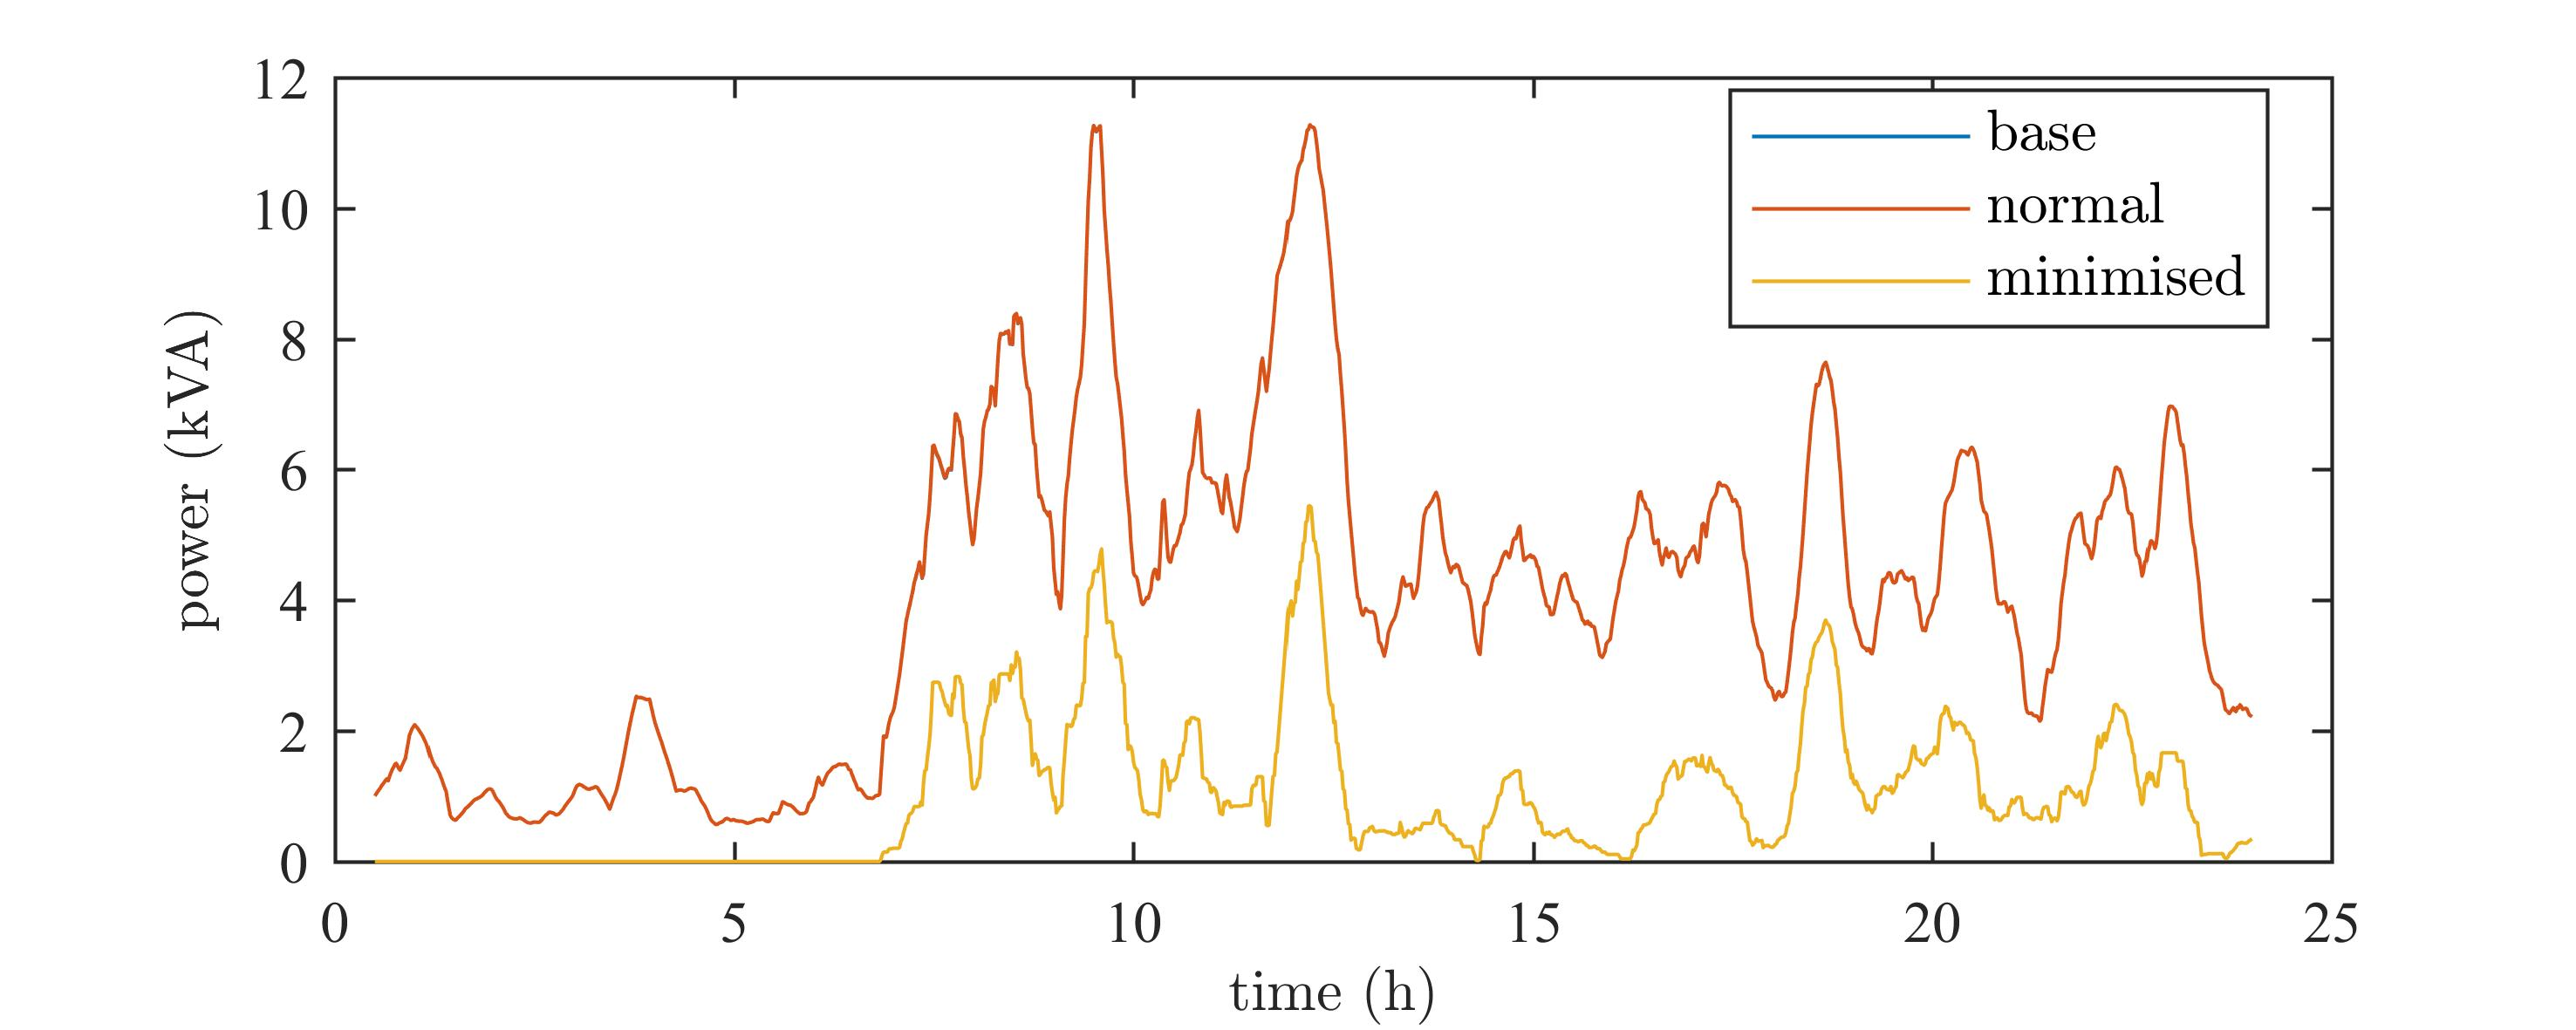
\includegraphics[width=\textwidth]{_chapter1/fig/ts-neutral-power-2}
\caption{Neutral power reduction due to the ESMU schedule adjustments}
\label{ch1:fig:ts-neutral-power}
\end{figure}

The results plotted in Figure \ref{ch1:fig:ts-neutral-power} show the network impact when adjusting the ESMU's schedule in order to minimise neutral power flow.
Incidentally, when applying the normal half-hourly ESMU schedule, neutral power is not affected at all.
The reason behind this was the choice of evenly assigning the scheduled power to all three phases, instead of taking into account the phases' loadings.
Power factor on the other hand was impacted just by introducing the half-hourly ESMU schedule, as shown in the following figure.

\begin{figure}\centering
	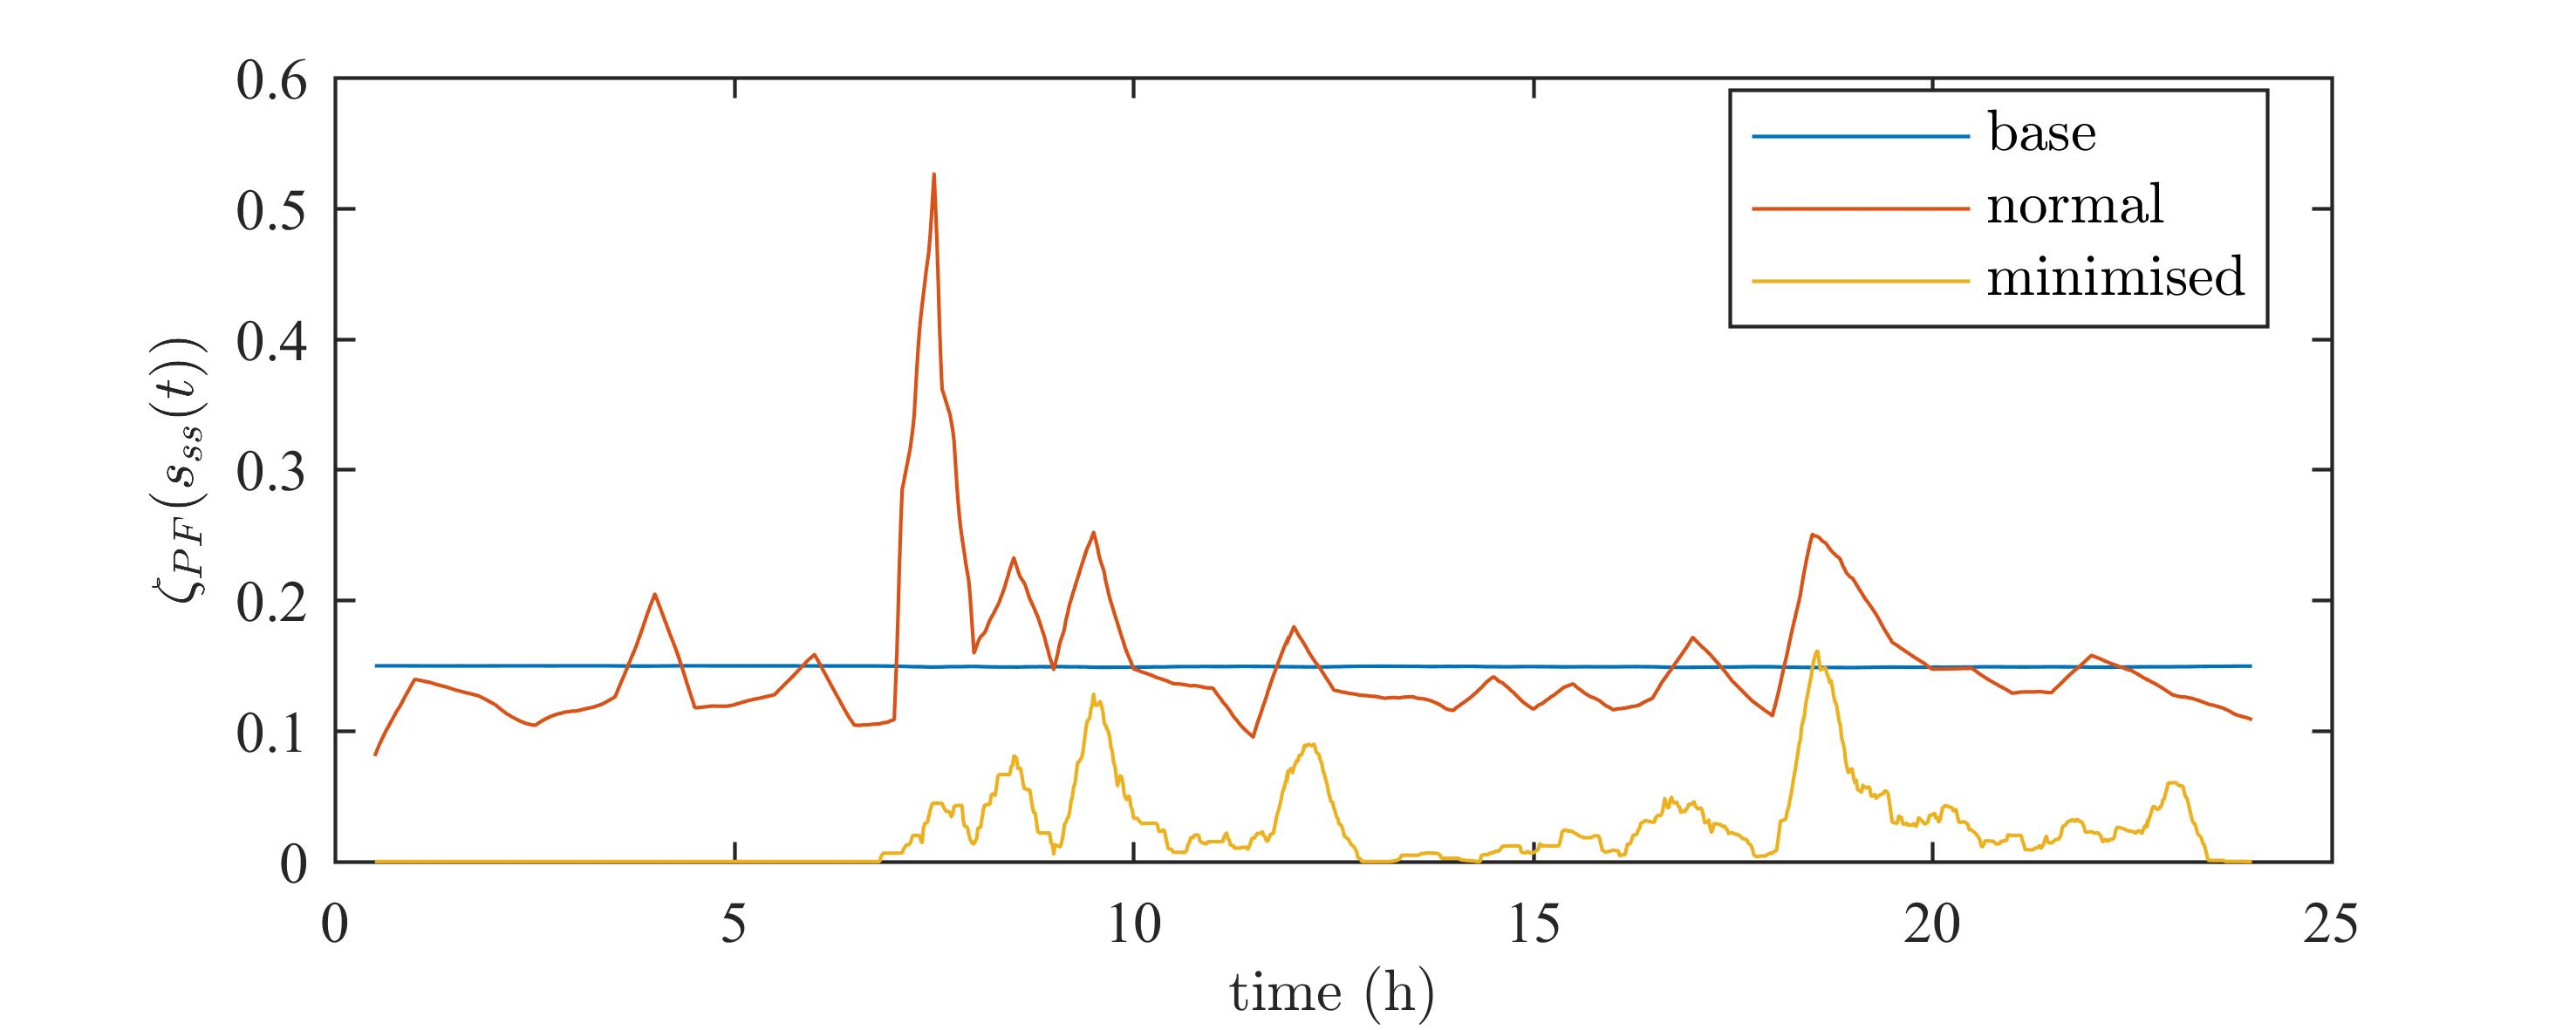
\includegraphics[width=\textwidth]{_chapter1/fig/ts-power-factor}
\caption{Power factor cost improvements due to the adjustment of the ESMU schedule}
\label{ch1:fig:ts-power-factor}
\end{figure}

Here, in Figure \ref{ch1:fig:ts-power-factor}, the power factor cost is successfully reduced during the entire day, in comparison to the normal cases.
In contrast, the base case had a constant power factor cost, due to aforementioned assignment of a constant power factor of 0.95 to all loads.
In reality, however, any network's power factor varies over time since the number of inductive machines and their associated inductive load varies constantly.
Nonetheless, the results would be similar but more variable when applied to a network with varying power factor, since the aim when adjusting the ESMU schedule was to reduce the power factor's deviation from unit power factor.
The final parameter that indicates system efficiency are the distribution losses.

\begin{figure}\centering
	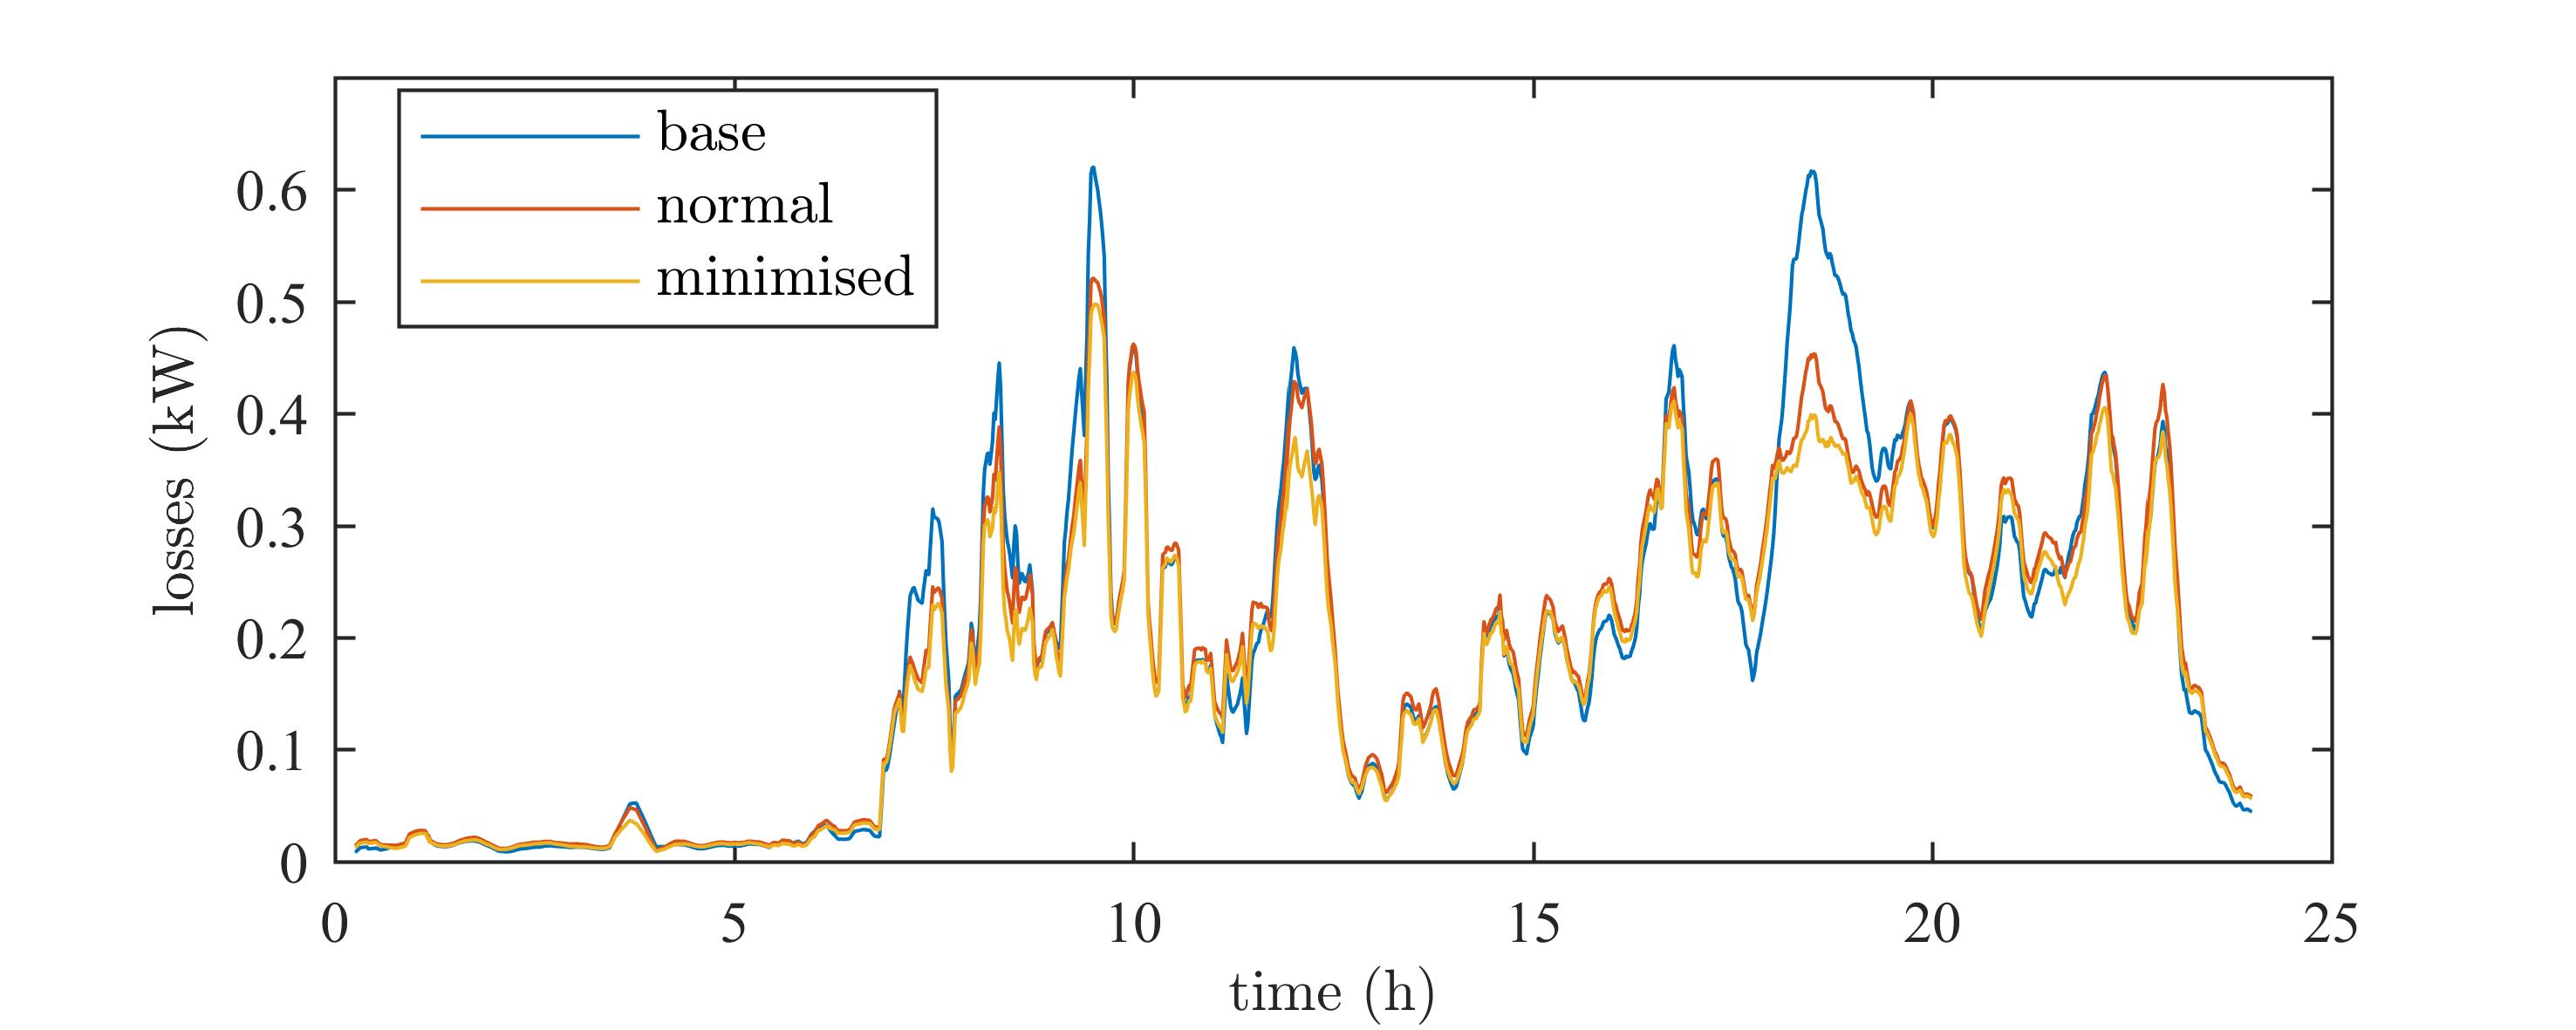
\includegraphics{_chapter1/fig/results/ts-losses_}
\caption{Instantaneous losses of the distribution network when adjusting the ESMU schedule in order to reduce the former \hl{(energy lost: 4.55kWh for base; 4.47kWh for normal; 4.19kWh for minimised)}.}
\label{ch1:fig:ts-losses}
\end{figure}

Figure \ref{ch1:fig:ts-losses} shows the reduction in distribution losses that were achieved when adjusting the ESMU schedule accordingly.
Again, the schedule adjustment reduced losses throughout the entire day.
In fact, an additional 6.42\% of energy savings could be achieved, simply by adjusting the ESMU's power injection and absorption behaviour.
Whilst this amount of energy may seem insignificant on a small scale, saving this amount of energy on a national level could potentially benefit the entire power network.
However, losses are difficult to measure and attempting to do so would most likely outweigh the benefits.

Instead, a better way of relieving stress from the power network is to minimise its assets utilisation by mitigating demand spikes.
Since the ESMU was constraint not to deviate from its underlying half-hourly schedule, only phase related demand differences could be addressed.
Those differences could however be addressed successfully, as shown in the following figure.

\begin{figure}\centering
	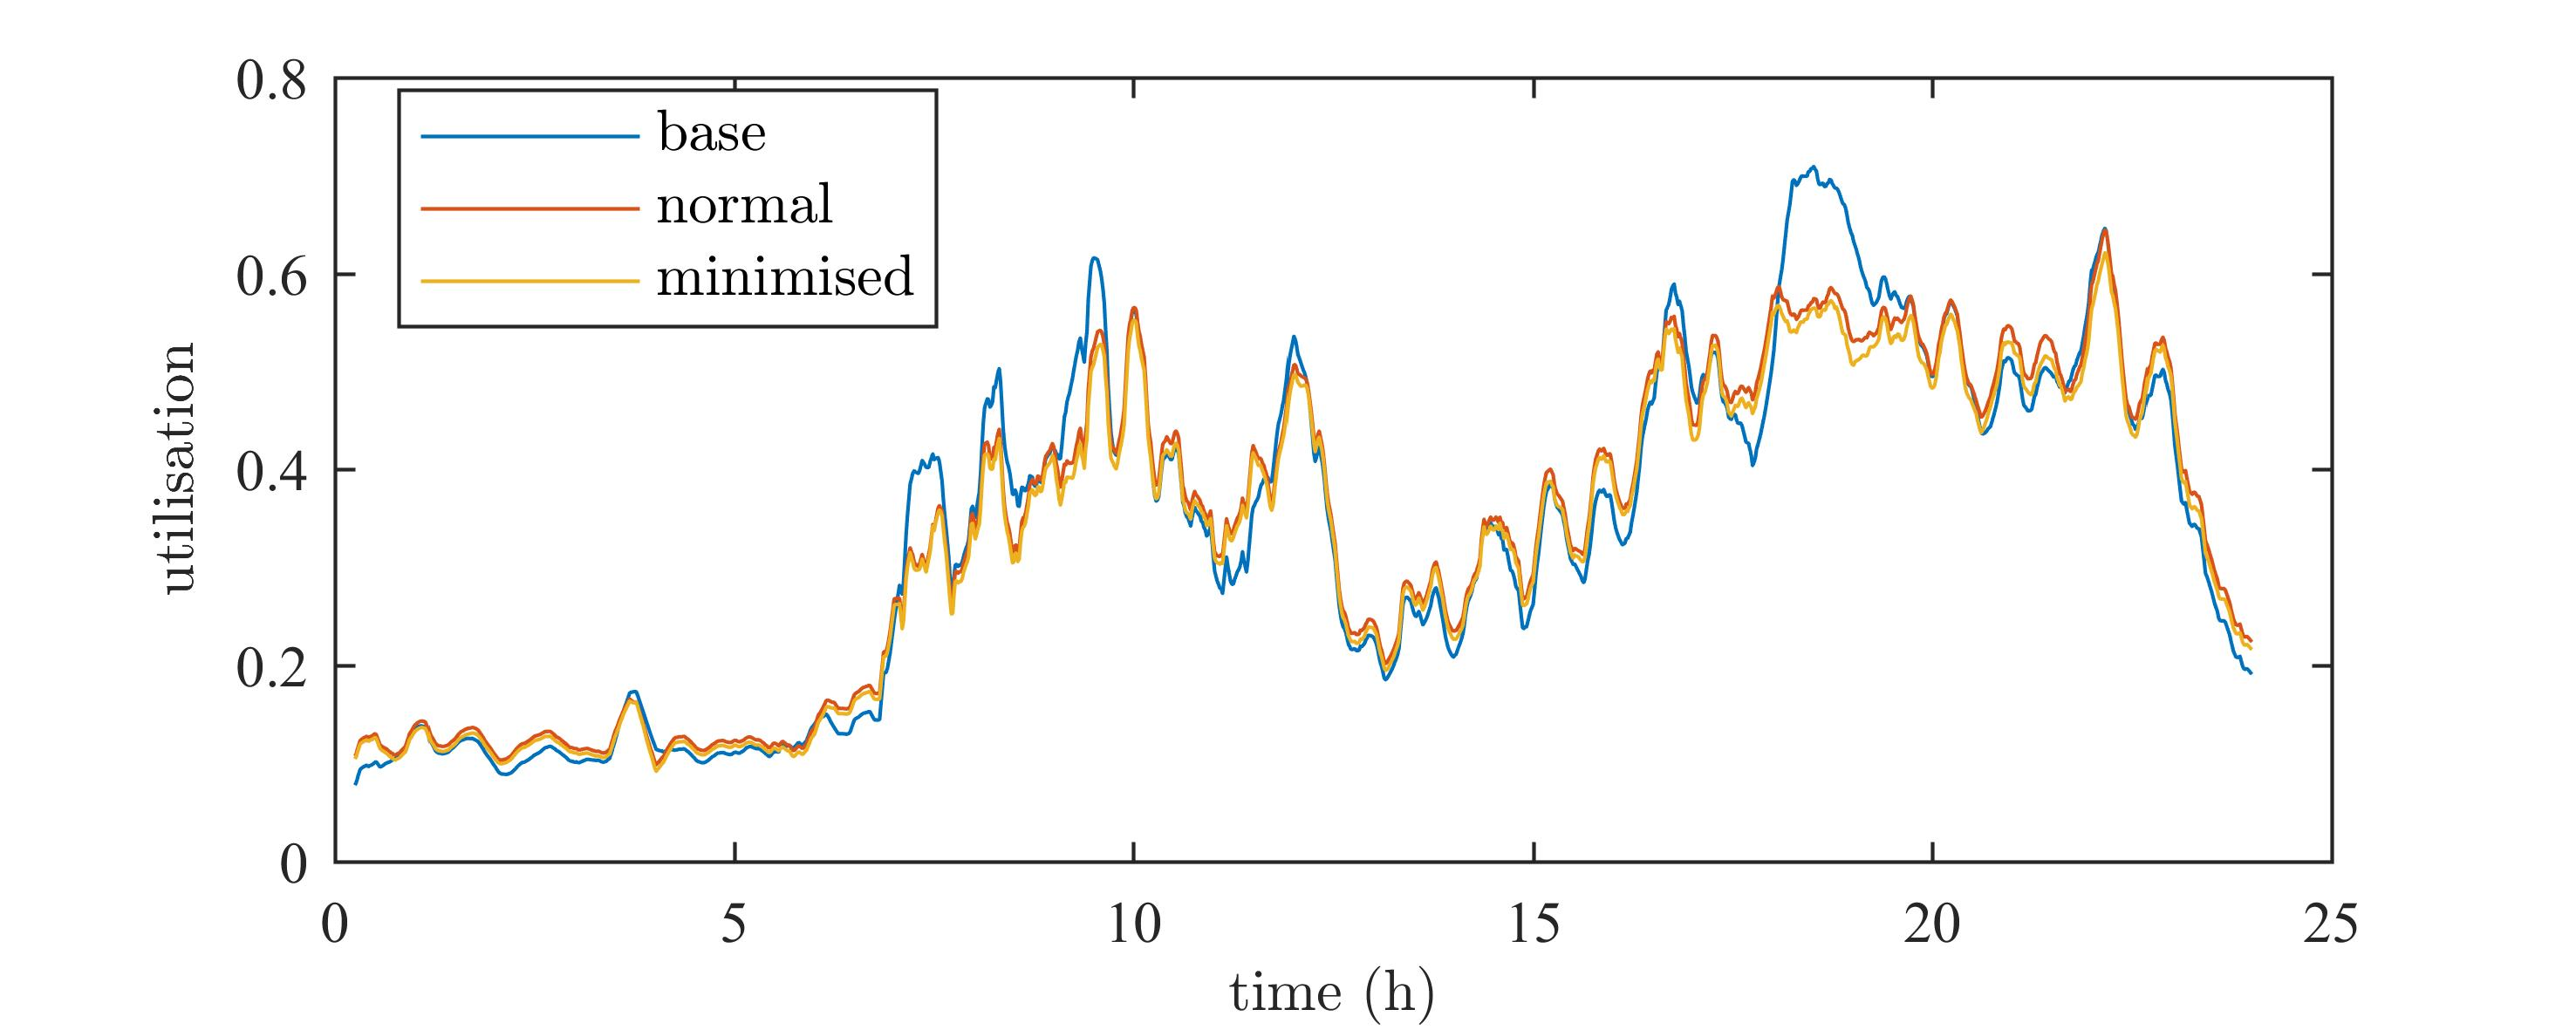
\includegraphics{_chapter1/fig/results/ts-all-line-utilisation_}
\caption{Improvement of the worst line utilisation across the entire network when adjusting the ESMU schedule correspondingly.}
\label{ch1:fig:ts-all-line-utilisation}
\end{figure}

Whilst the worst line utilisation is predominantly driven by the half-hourly charging and discharging behaviour of the ESMU, a subtle reduction could be achieved throughout the entire day, as shown in Figure \ref{ch1:fig:ts-all-line-utilisation}.
Yet as mentioned before, the constraint that is imposed due to the underlying half-hourly schedule significantly limits this improvement in network performance.

\subsection{Difference Analysis}
\label{ch1:subsec:difference-analysis}

In order to gage the whether the is a statistical difference in network performance, a box-plot was generated for each case.
The underlying data for each box-plot is the paired difference between the corresponding case's costs and the associated normal case's costs, i.e. when letting the ESMU operate normally, without adjusting its schedule.
Any positive difference in those costs indicates an improvement to the system's performance, whilst a negative difference would imply a worsening.

Here, the improvements for each individual cost are compared and plotted in Figure \ref{ch1:fig:boxplot-overall-improvements}.
A further set of comparing figures is also included in Appendix Section \ref{appx-a:ch1:additional-difference-analysis}, where the impacts on all costs, when minimising a for only an individual cost are compared.
Instead of including all these figures in the main body of this Thesis, the sum of all costs is computed and included in a table to give a more comprehensive indication of these so called cross-cost improvements.

\begin{figure}\centering
	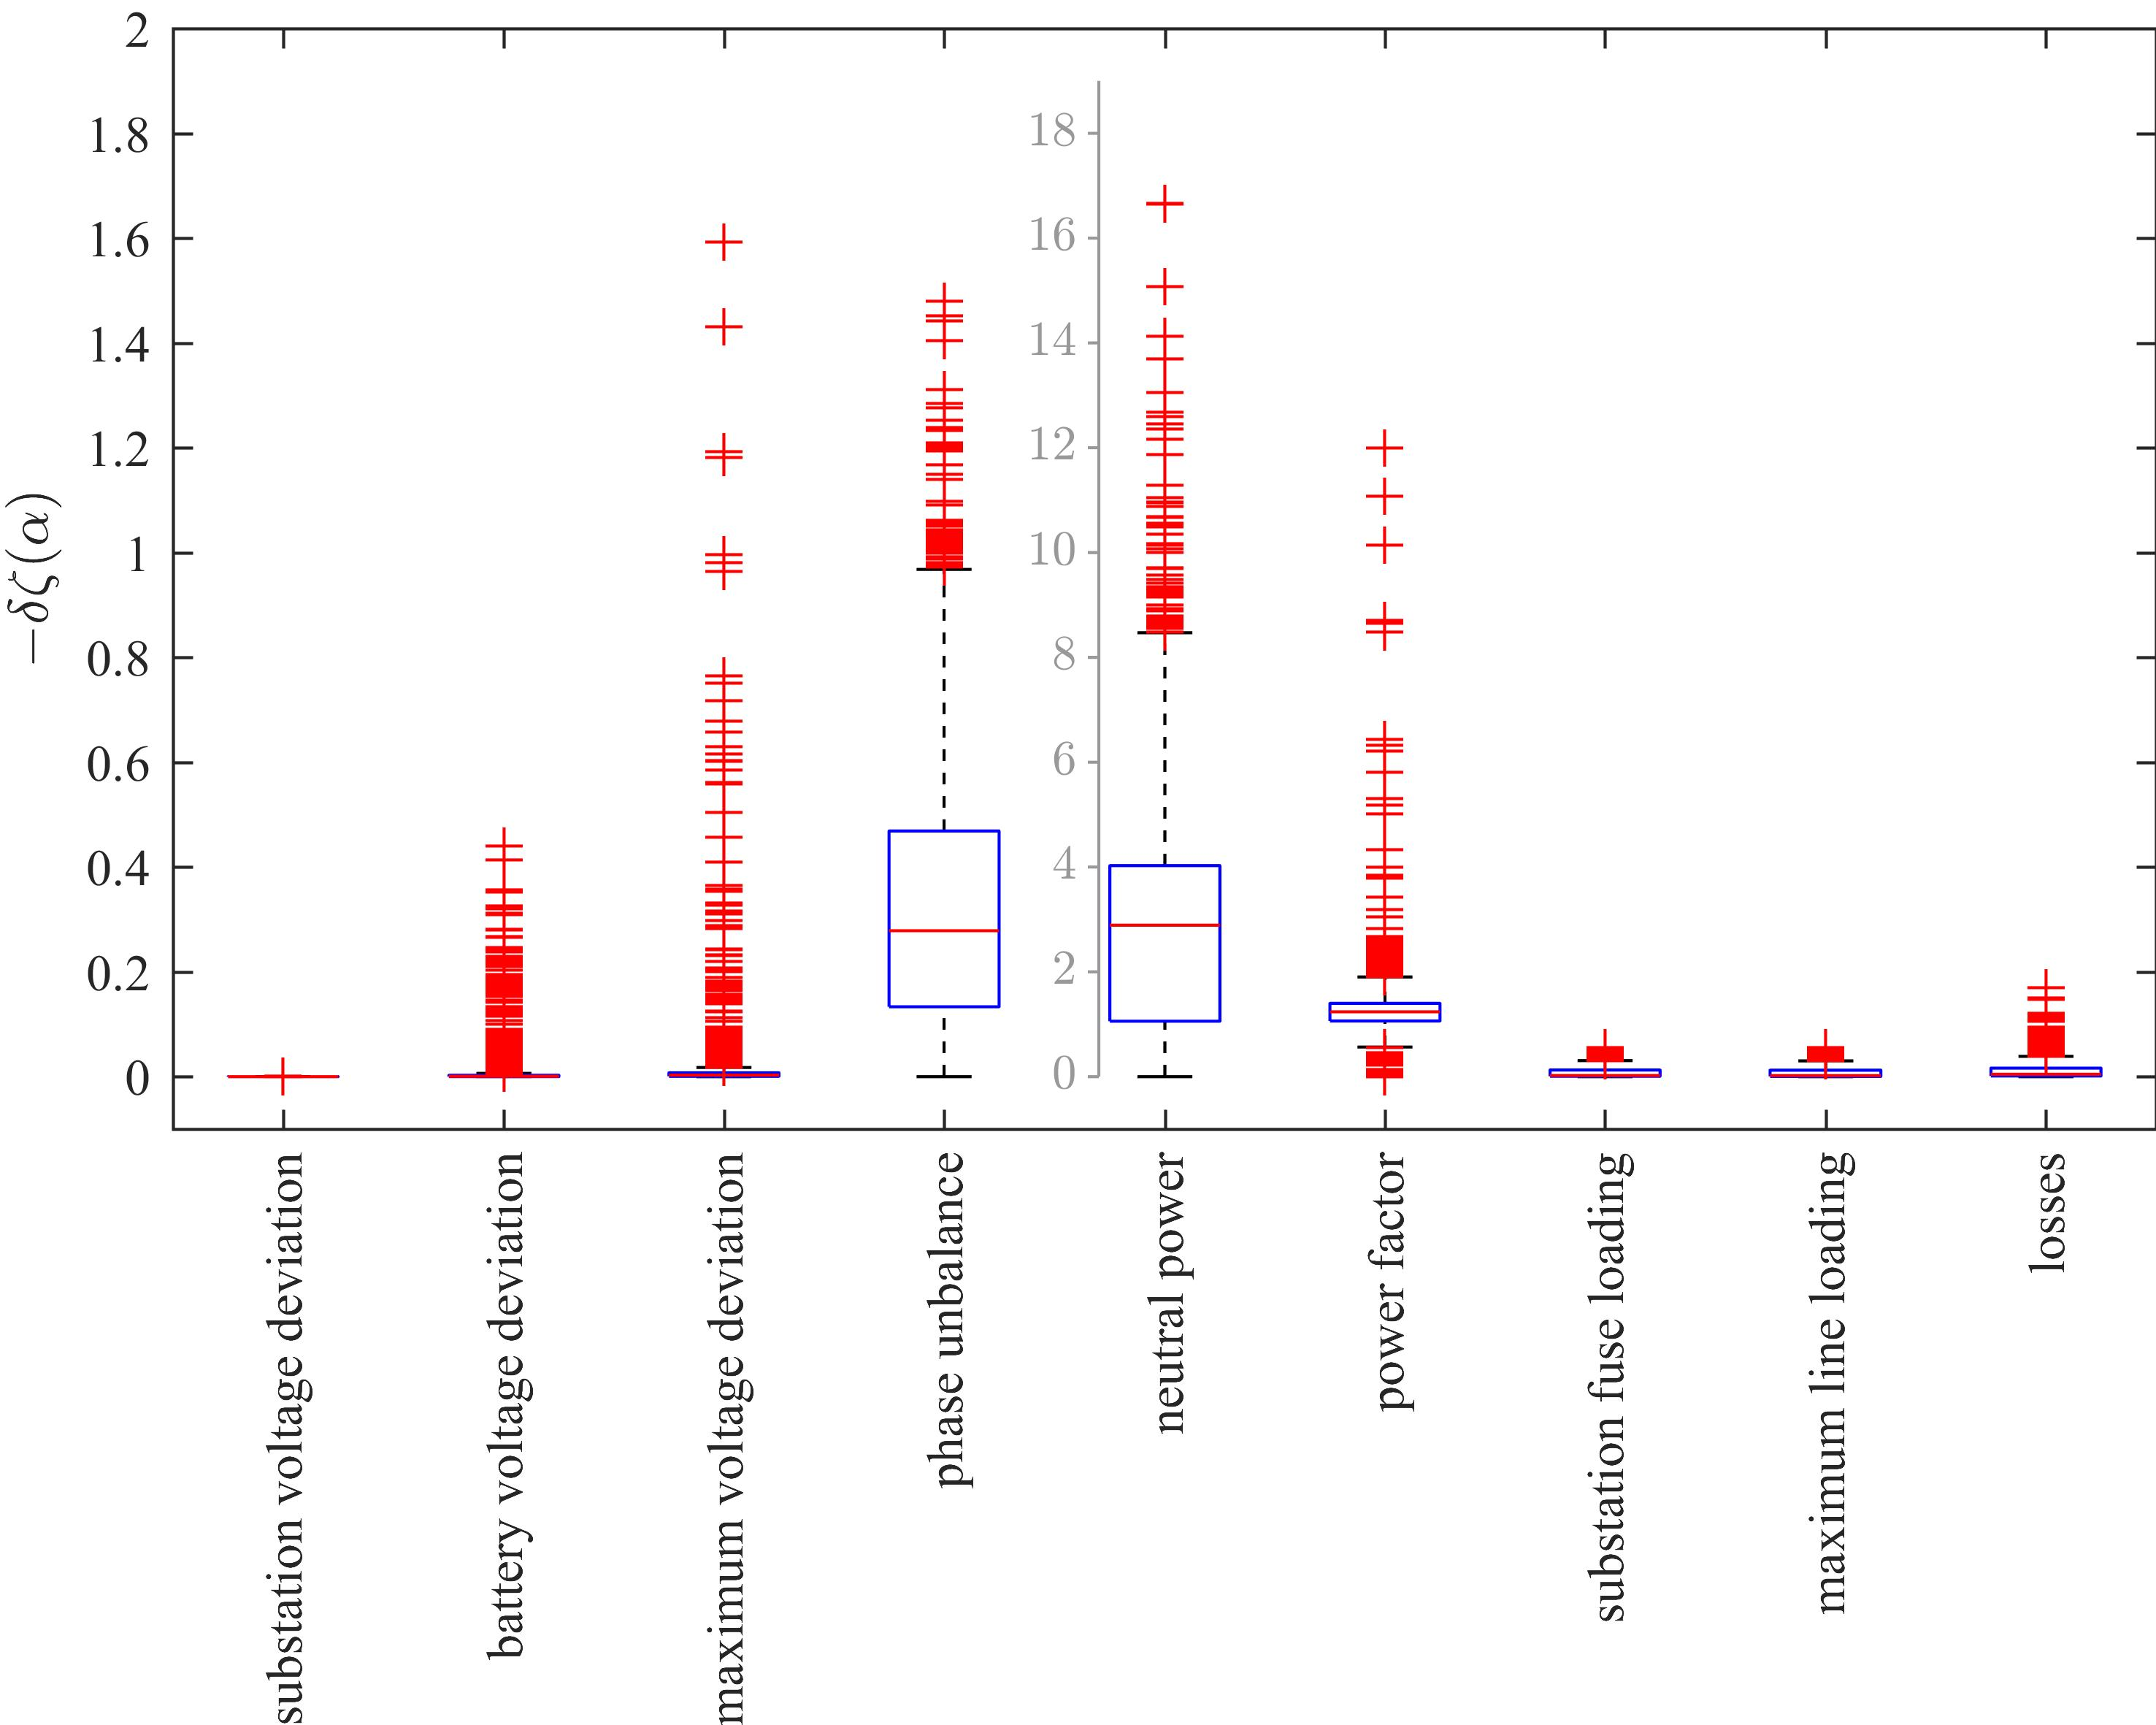
\includegraphics[width=\textwidth]{_chapter1/fig/results/boxplot-overall-improvements}
\caption{Cost-function improvement spread, when comparing against the normal ESMU operation case and when optimising for the underlying cost (a separate y-axis is introduced for the optimisation of ``neutral power'').}
\label{ch1:fig:boxplot-overall-improvements}
\end{figure}

In Figure \ref{ch1:fig:boxplot-overall-improvements}, it can be seen that the most significant cost related impact on the network was on the improvement of phase unbalance, neutral power and power factor.
The reason for this noticeably larger impact is that the ESMU can assign its scheduled active power in an arbitrary manner to all three phases, as long as the predetermined half-hourly schedule is followed.
It is this constraint of having to obey the schedule, that limits the impact on all other key network parameters.
Reactive power on the other hand is not directly limited to this constraint, since it is not scheduled as such.
The only limit that applies to the ESMU's reactive power injection capabilities, is the remaining PMU capacities when applying the active powers in order to follow the half-hourly schedule.
Also, unlike active power, reactive power has a smaller impact on the LV network due to its physical property, i.e. being more resistive than inductive.
Nonetheless, all key network parameters were impacted positively when they became subject to their associated cost-function minimisation.

To summarise the aforementioned cross-cost improvements (which are presented in detail in the Appendix, Section \ref{appx-a:ch1:additional-difference-analysis}), all costs are calculated for all minimisation cases, compared against the normal case, and accumulated into a single value.
This value is defined as the ``cumulative cost difference''.
Additionally, the normal case is compared to the base case in a similar manner.
This was done since it is interesting to see how the half-hourly schedule impacted the network.

\begin{sidewaystable}\centering
\definecolor{light_blue}{rgb}{0.9, 0.9, 1.0}
\definecolor{dark_blue}{rgb}{0.5, 0.5, 1.0}
\begin{tabular}{cc|ccccccccc|}
& & \multicolumn{9}{c}{minimisation cases} \\
& \rotatebox[origin=l]{90}{normal}& \rotatebox[origin=l]{90}{substation voltage deviation}& \rotatebox[origin=l]{90}{battery voltage deviation}& \rotatebox[origin=l]{90}{maximum voltage deviation}& \rotatebox[origin=l]{90}{phase unbalance}& \rotatebox[origin=l]{90}{neutral power}& \rotatebox[origin=l]{90}{power factor}& \rotatebox[origin=l]{90}{substation fuse loading}& \rotatebox[origin=l]{90}{maximum line loading}& \rotatebox[origin=l]{90}{losses} \\
\hline
\multicolumn{1}{r|}{substation voltage deviation} & 0.00 & \cellcolor{light_blue}0.08 & -2.49 & -1.39 & -4.89 & -8.72 & \cellcolor{light_blue}0.04 & 0.00 & \cellcolor{light_blue}0.01 & -1.09 \\
\multicolumn{1}{r|}{battery voltage deviation} & -5.01 & -0.40 & \cellcolor{light_blue}15.52 & \cellcolor{light_blue}17.04 & \cellcolor{light_blue}9.14 & \cellcolor{light_blue}14.93 & -2.85 & -0.43 & -1.62 & \cellcolor{light_blue}13.69 \\
\multicolumn{1}{r|}{maximum voltage deviation} & -6.83 & -1.15 & \cellcolor{light_blue}28.22 & \cellcolor{light_blue}36.42 & \cellcolor{light_blue}24.66 & \cellcolor{light_blue}33.05 & -3.07 & -0.56 & -2.57 & \cellcolor{light_blue}25.44 \\
\multicolumn{1}{r|}{phase unbalance} & \cellcolor{light_blue}12.15 & \cellcolor{light_blue}40.93 & \cellcolor{light_blue}284.87 & \cellcolor{light_blue}380.57 & \cellcolor{light_blue}490.22 & \cellcolor{light_blue}351.35 & \cellcolor{light_blue}40.66 & \cellcolor{light_blue}10.02 & \cellcolor{light_blue}5.03 & \cellcolor{light_blue}441.24 \\
\multicolumn{1}{r|}{neutral power} & -0.83 & -96.72 & \cellcolor{light_blue}2303.70 & \cellcolor{light_blue}1642.37 & \cellcolor{light_blue}2698.78 & \cellcolor{light_blue}4415.85 & \cellcolor{light_blue}319.23 & \cellcolor{light_blue}133.46 & \cellcolor{light_blue}53.53 & \cellcolor{light_blue}2401.12 \\
\multicolumn{1}{r|}{power factor} & -0.27 & \cellcolor{light_blue}159.42 & -7.63 & -37.25 & -633.30 & -314.11 & \cellcolor{light_blue}183.01 & \cellcolor{light_blue}145.35 & \cellcolor{light_blue}136.87 & \cellcolor{light_blue}88.84 \\
\multicolumn{1}{r|}{substation fuse loading} & \cellcolor{light_blue}5.14 & \cellcolor{light_blue}13.34 & -0.43 & -8.69 & -51.76 & -72.68 & \cellcolor{light_blue}14.37 & \cellcolor{light_blue}10.98 & \cellcolor{light_blue}10.91 & \cellcolor{light_blue}5.64 \\
\multicolumn{1}{r|}{maximum line loading} & \cellcolor{light_blue}4.53 & \cellcolor{light_blue}12.88 & -6.17 & -10.04 & -80.41 & -97.30 & \cellcolor{light_blue}13.89 & \cellcolor{light_blue}10.69 & \cellcolor{light_blue}10.94 & \cellcolor{light_blue}4.72 \\
\multicolumn{1}{r|}{losses} & \cellcolor{light_blue}4.34 & \cellcolor{light_blue}7.22 & \cellcolor{light_blue}13.38 & -4.46 & -46.37 & -66.32 & \cellcolor{light_blue}12.89 & \cellcolor{light_blue}9.65 & \cellcolor{light_blue}9.02 & \cellcolor{light_blue}17.13 \\
\end{tabular}
\caption{Cross-cost improvements due to adjustments to the original ESMU schedule.}
\label{ch1:tab:cost-table}
\end{sidewaystable}


The cumulative cost differences are tabulated in Table \ref{ch1:tab:cost-table}.
Every improvement in system operation is reflected as a reduction in cost, when compared to the corresponding normal or base case.
Therefore, a positive cumulative cost difference indicates, that over an entire day, the system operation improved in regards to the given cost.
Here, these improvements, i.e. positive cumulative cost differences, have been highlighted.

As expected, all entries along the diagonal, i.e. where the evaluated cost is also the cost that was minimised for the underlying case, nearly always show the largest cumulative cost differences.
It is also interesting to see, how a specific cost minimisation had noticeable impacts on different cumulative cost measures.
For example, adjusting the ESMU schedule to achieve the largest reduction in distribution losses (i.e. far right column) had an impact on all key network parameters.
This impact was also positive in nature for all key network parameters (apart from substation voltage deviation).

Then again, although the network optimisation for an optimised line and fuse loading did result in a positive cumulative cost difference, reduction in power factor had a more significant positive impact.
The reason behind this is that instantaneous apparent power contributes to the loading.
This means, that increasing the power factor inadvertently reduces reactive load, which in turn lowers the total current flowing into the system.
Not knowing what cost to address first, makes it difficult for the used solving algorithm to find the global minimum.
To improve the performance of the adjusted ESMU schedule, one could concatenate the cost minimisation in series to locate regions where lower minima may be found.
In this case at least, maximising the network's power factor before addressing fuse and line utilisation would have been a better choice.

\subsection{Probability Density Analysis}
\label{ch1:subsec:probability-density-analysis}

The final part of analysing the results is to statistically determine, whether the cumulative cost differences are indeed significantly different.
To do so, the probability density functions (PDF) of the  cost differences is analysed using a null hypothesis test.
However, the underlying data had to be conditioned in order to meet all prerequisites that are necessary to perform a null hypothesis test, such as the standard $t$-test.
These prerequisites include stationarity, low auto-correlation and high gaussianity of the underlying time-series.
The conditioning to meet such these prerequisites had to be carried out without falsifying the data, therefore limiting possible operations to time-series division and linear transformations.
Details on the exact steps are outside the scope of this chapter, yet have been included in the appendix for completeness.

\begin{sidewaystable}\centering
\definecolor{light_blue}{rgb}{0.9, 0.9, 1.0}
\definecolor{dark_blue}{rgb}{0.5, 0.5, 1.0}
\definecolor{light_red}{rgb}{1.0, 0.5, 0.5}
\begin{tabular}{cc|ccccccccc|}
& & \multicolumn{9}{c}{minimisation cases} \\
& \rotatebox[origin=l]{90}{normal}& \rotatebox[origin=l]{90}{substation voltage deviation}& \rotatebox[origin=l]{90}{battery voltage deviation}& \rotatebox[origin=l]{90}{maximum voltage deviation}& \rotatebox[origin=l]{90}{phase unbalance}& \rotatebox[origin=l]{90}{neutral power}& \rotatebox[origin=l]{90}{power factor}& \rotatebox[origin=l]{90}{substation fuse loading}& \rotatebox[origin=l]{90}{maximum line loading}& \rotatebox[origin=l]{90}{losses} \\
\hline
\multicolumn{1}{r|}{substation voltage deviation} & $0.851$ & \cellcolor{light_blue}$<0.001$ & $0.999$ & $1.000$ & $0.999$ & $1.000$ & \cellcolor{light_blue}$<0.001$ & \cellcolor{light_blue}$<0.001$ & \cellcolor{light_blue}$<0.001$ & $0.999$ \\
\multicolumn{1}{r|}{battery voltage deviation} & $0.899$ & \cellcolor{light_blue}$<0.001$ & \cellcolor{light_blue}$<0.001$ & \cellcolor{light_blue}$<0.001$ & \cellcolor{light_blue}$<0.001$ & \cellcolor{light_blue}$<0.001$ & \cellcolor{light_blue}$0.022$ & \cellcolor{light_blue}$0.018$ & $0.325$ & \cellcolor{light_blue}$<0.001$ \\
\multicolumn{1}{r|}{maximum voltage deviation} & $0.718$ & \cellcolor{light_blue}$0.000$ & \cellcolor{light_blue}$<0.001$ & \cellcolor{light_blue}$<0.001$ & \cellcolor{light_blue}$<0.001$ & \cellcolor{light_blue}$<0.001$ & $0.086$ & $0.167$ & $0.772$ & \cellcolor{light_blue}$<0.001$ \\
\multicolumn{1}{r|}{phase unbalance} & $0.331$ & \cellcolor{light_blue}$<0.001$ & \cellcolor{light_blue}$<0.001$ & \cellcolor{light_blue}$<0.001$ & \cellcolor{light_blue}$<0.001$ & \cellcolor{light_blue}$<0.001$ & \cellcolor{light_blue}$<0.001$ & \cellcolor{light_blue}$0.001$ & \cellcolor{light_blue}$0.038$ & \cellcolor{light_blue}$<0.001$ \\
\multicolumn{1}{r|}{neutral power} & $0.940$ & $0.999$ & \cellcolor{light_blue}$<0.001$ & \cellcolor{light_blue}$<0.001$ & \cellcolor{light_blue}$<0.001$ & \cellcolor{light_blue}$<0.001$ & \cellcolor{light_blue}$<0.001$ & \cellcolor{light_blue}$<0.001$ & \cellcolor{light_blue}$0.016$ & \cellcolor{light_blue}$<0.001$ \\
\multicolumn{1}{r|}{power factor} & $0.488$ & \cellcolor{light_blue}$<0.001$ & \cellcolor{light_blue}$0.020$ & $0.999$ & $0.999$ & $1.000$ & \cellcolor{light_blue}$<0.001$ & \cellcolor{light_blue}$<0.001$ & \cellcolor{light_blue}$<0.001$ & \cellcolor{light_blue}$<0.001$ \\
\multicolumn{1}{r|}{substation fuse loading} & $0.777$ & \cellcolor{light_blue}$<0.001$ & $0.929$ & $0.999$ & $0.999$ & $1.000$ & \cellcolor{light_blue}$<0.001$ & \cellcolor{light_blue}$<0.001$ & \cellcolor{light_blue}$<0.001$ & \cellcolor{light_blue}$0.001$ \\
\multicolumn{1}{r|}{maximum line loading} & $0.846$ & \cellcolor{light_blue}$<0.001$ & $0.996$ & $0.999$ & $0.999$ & $0.999$ & \cellcolor{light_blue}$<0.001$ & \cellcolor{light_blue}$<0.001$ & \cellcolor{light_blue}$<0.001$ & $0.102$ \\
\multicolumn{1}{r|}{losses} & $0.881$ & \cellcolor{light_blue}$<0.001$ & \cellcolor{light_blue}$<0.001$ & $0.637$ & $0.910$ & $0.999$ & \cellcolor{light_blue}$<0.001$ & \cellcolor{light_blue}$<0.001$ & \cellcolor{light_blue}$<0.001$ & \cellcolor{light_blue}$<0.001$ \\
\end{tabular}
\caption{$p$-values for statistical evidence of cross-cost improvements based on statistical two-sample single-tailed $t$-test.}
\label{ch1:tab:t-test-table}
\end{sidewaystable}


Table \ref{ch1:tab:t-test-table} presents the results from this analysis.
Here, $p$-values have been tabulated and those cells with a value below $0.05$ are highlighted in blue.
A similar pattern to that in the previous table seen, where the cumulative cost difference was tabulated.
Here however, instead of just comparing costs, statistical indications to support the significance of the findings is presented, here.
In combination with the preceding table, one can determine that e.g. the impact of optimising operation based on maximum voltage deviation has little to no significant impact on improvements in power factor.
The most critical finding is however, that each cost minimisation did indeed result in significant improvement of corresponding network operation.


\section{Summary}
\label{ch1:sec:summary}

In this chapter, a method to adjust three-phase ESMU powers on a sub-half-hourly basis to support network operation, whilst following a pre-determined half-hourly schedule, is proposed and tested.
The ESMU schedule is tailored to result in a ``peak-shaving'' and ``valley-filling'' behaviour and uses a realistic ESMU model to meet any operational constraints.
A set of key network parameters to indicate the performance of the network, were used in a corresponding set of cost functions.
By adjusting the ESMU's active and reactive powers, each cost could be minimised and therefore network operation is improved.

Results indicate that when explicitly focusing on the improvement of certain key network parameters, then the derived cost reduces for every single case.
Nonetheless, any cost minimisation had an effect on different costs (e.g. loss minimisation positively impacted nearly all other costs).
Using cumulative cross-cost differences, it is shown that a net cost reduction is achieved, simply by implementing the proposed ESMU power adjustment method top of the normal execution of a half-hourly schedule.
This fact is also supported by the statistical sensitivity analysis, using the two-paired $t$-test.
Using this test after having correctly preconditioned the data to meet the test's prerequisites, the initial null hypothesis is successfully be disproven; i.e. the hypothesis that sub-half hourly power adjustments have no impact.
Hence there is strong evidence that those power adjustments do have a positive impact on the distribution network's operation, and the first objective of this thesis, which is outlined in Section~\ref{ch-introduction:sec:problem-statement}, has been met.

The main limitation of the proposed method is however the battery's half-hourly schedule.
It dictates the active power that has to be injected into or absorbed from the distribution network.
Also, this schedule inadvertently dictates the remaining overhead in reactive power that may be compensated for on each phase.
Therefore, the next chapter in this thesis presents a method of dynamically adjusting this scheduled power profile in real-time without violating any physical constraints.

\chapter{Real-Time Adjustment of Battery Operation using MPC Guided Schedule Deviation}
\label{ch2}

%\singlespacing
%\epigraph{\textit{M. J. Zangs, et al., ``Battery control algorithm for peak load shaving in low-voltage power network with high demand volatility,'' Applied Energy}}{--- Unpublished}
%\doublespacing

\section{Overview}
\label{ch2:sec:overview}

%Outages are still very frequent in the UK. 
%According to the UK energy regulator \textit{OFGEM}, on average 45\% of all customers experienced service disruptions in the period 2015-16 \cite{Ofgem2017}.
%Whilst unanticipated outages due to severe winter weather lead to \pounds39 million worth of damages \cite{Ofgem2014}, network upgrades and repairs however contributed the larger amount of customer interruptions and customer minutes lost.
%Such planned outages are intentions to strengthen networks and mitigate system overloads, due to increasing demand for electricity.
%This demand increase is only accelerated since major focus of UK energy policies has been put on transitioning towards a low carbon economy \cite{HMGovernment2009, RoyalAcademyofEngineering2010}.
%Particularly the decarbonisation of heat and transport sectors are two areas of significant strategic focus and Low Carbon Technology (LCT) such as photovoltaic installations, electric vehicles and heat pumps are expected to contribute significantly to this transition.
%
%However, as adaptation of these LCTs increases and they start to penetrate power distribution networks, stress on these networks will continue to increase even further, which may result in additional service disruptions.
%Furthermore, the uptake of LCTs is not expected to progress evenly throughout the entire power network, and instead clusters of early adopters are predicted to form, leading to certain Low-Voltage (LV) networks to exceed their operational constraints even at relatively low national rate of LCT adaption \cite{Poghosyan2014}.
%Traditional network planning approaches to circumvent constraint violations, follow the commonly used practice of aggregating a large number of customers and designing the power delivery network to cater for their largest probable demand, i.e. the After Diversity Maximum Demand (ADMD) method \cite{Richardson2010a}.
%This ADMD method has remained the same for many years and uses historical load analysis and standard growth assumptions that are both no longer valid in this unprecedented LCT uptake scenario \cite{Yunusov2016}.
%To make things worse, LV networks in the UK are generally unmonitored once installed.
%Distribution Network Operators (DNOs) have become aware of this issue and are developing updated planning strategies involving ``smart'' and ``flexible'' electricity grids.
%However, in situ equipment that will become subject to the same adaptation of LCT needs to be managed actively via innovation in the use of existing and new technologies; otherwise both frequency of service disruptions and customer minutes lost will increase alongside the proliferation of LCTs \cite{Ault2008a}.
%
%Two solutions exist, allowing DNOs to support LV network's operation: 
%\begin{enumerate*}
%	\item reinforcement of in situ network assets;
%	\item deployment of network support equipment.
%\end{enumerate*}
%Whilst network reinforcement would certainly address immediate issues of current network capacity constraints, it is also the more expensive and disruptive option.
%More specifically, customer will need to deal with outages during periods of asset upgrades (e.g. transformer upgrade and line re-conductoring after secondary transformers' tap settings have been adjusted).
%Therefore, alternatives to defer or avoid network reinforcements have been sought and assessed \cite{Harrison2007, Zangs2016a, VanderKlauw2016d, Greenwood2017}.
%Most promising alternatives are to install flexible and controllable Distributed Energy Resources (DERs), or more specifically: Battery Energy Storage Solutions (ESMU) \cite{Wade2010}.
%ESMU has not only seen significant advancements in technology, but also received increasing attention in both academic studies and industry trials \cite{Palizban2016}.
%
%Installing ESMU on a strategic location in the LV network brings several advantages to DNOs' control over the network's performance.
%Regulating voltages to stay within statutory operating bands \cite{Yang2014}, shaving peak load to relieve stress from the installed network assets \cite{Bennett2015}, or reducing phase unbalance to increase network efficiency \cite{Wang2015b} are only a few examples of recent research in this field.
%Whilst the questions regarding locating and scaling of ESMU have mostly been addressed, ESMU control can be split into two complementing yet unmarried approaches:
%\begin{enumerate*}
%	\item ``off-line'' control, using load forecasts and ESMU schedules; and
%	\item ``on-line'' control, using Set-Points Control (SPC), Model Predictive Control (MPC) or similar dynamic control methods.
%\end{enumerate*}
%
%Off-line control uses historic data to predict future load patterns, which are used to schedule ESMU operation accordingly.
%Early approaches, e.g. by Oudalov et al. \cite{Oudalov2007}, who used dynamic programming to generate ESMU schedules, had a relatively high forecast error due to the inherent difficulty of predicting future loads, which ultimately limits the ability of given ESMU schedule to i.e. reduce peaks.
%This reason is why recent research either includes uncertainty, like the work by Baker et al. \cite{Baker2017} where uncertainty of wind power was taken into account when scheduling and sizing ESMU, or it frequently re-evaluates ESMU schedules, as done by Wang et.al \cite{Wang2014a}, where ESMU control is adjusted after each decision epoch.
%Despite load forecasts being imperfect, forecasts remain a key component for scheduling ESMU thanks to work like that by Rowe et al. \cite{Rowe2014a}, where a filtering mechanism was proposed for scheduling algorithms to reduce peak load in LV networks in spite of forecast errors.
%Furthermore, most day-ahead forecast only forecast at a temporal resolution down to half-hourly periods.
%As pointed out by Haben et al. \cite{Poghosyan2014, Haben2014}, forecasts at half-hourly resolution yield the best compromise between high accuracy and high temporal resolution, which is why they have become the standard for generating ESMU operating schedules.
%Nonetheless, sub-half-hourly load volatility imposes the biggest stress on the network and cannot be addressed when using this kind of half-hourly forecast, which is why on-line control has been considered as an alternative to off-line control.
%
%One flavour of on-line control is the Set-Point Control (SPC), which is a robust technique that can immediately respond to network changes.
%Since this kind of control runs the risk of reaching shortage or surplus of ESMU stored energy, modifications like hysteresis control \cite{Gybel2012} and ramp-rate control \cite{Such2012} were proposed.
%However, this kind of on-line control is less effective in addressing daily demand peaks, since pure SPC can only react to current network demand and does not respond to general trends or upcoming load events.
%To address these shortcomings SPC has been extended, using short-term load predictions by implementing Model Predictive Control (MPC).
%Some MPC examples include Auto-Regressive (AR) models \cite{Li2009, Nie2011}, fuzzy logic models \cite{Sannomiya2001, Chen2013a}, genetic algorithms \cite{Xia2015a, Liu2015} or Artificial Neural Networks (ANN) \cite{Kalogirou2014, Quan2014, Lee2014, Pezeshki2014, Vaz2016, Reihani2016, Xiao2017}.
%Implementing increasingly complex MPC to support on-line control is therefore a strong research trend, however the computational burden to deliver real-time solutions makes implementation of such systems not yet feasible.

\nomenclature[G]{SPC}{Set-Point Control}
\nomenclature[G]{MPC}{Mode-Predict Control}
\nomenclature[G]{PID}{Proportional Integrating Derivative (control)}


In the preceding chapter an Energy Storage Management Unit (ESMU) is used to improve network operation.
This improvement is achieved by optimally adjusting the device's scheduled three-phase powers.
Any improvement is indicated by reduction of cost functions, which are tied to key network parameters.
By focusing on different costs and repetitively optimising and simulating the ESMU powers, shows the extend by which the device can improve the network's operation.
However, this improvement is limited by the constraint of having to obey the underlying half-hourly ESMU schedule, despite applying adjustments at a sub-half-hourly level.

In the following chapter, this limiting constraint is lifted, and the corresponding sub-half-hourly ESMU schedule adjustment method is proposed.
This method unifies the benefits from sub-half-hourly demand measurements and half-hourly demand forecasts.
Unlike previous work in the field, the proposed approach reverses the traditional control paradigm to compensate for schedule inaccuracies.
To reiterate, these traditional approaches implemented on-line control mechanisms, e.g. Set-Point Control (SPC), in combination with prediction models in order to adjust and prepare ESMU for future load trends.
In this presented work however, instead of supporting on-line control with real-time load predictions, forecast driven schedules are adjusted using on-line measurements.
This is achieved by first scheduling ESMU operation at half-hourly resolution, i.e. by following a ``peak-shaving'' and ``valley-filling'' behaviour which has been explained in Chapter \ref{ch1}, and then modifying this schedule using MPC.
In this case, MPC is comprised of of a lightweight AR model to assure real-time deployability.
These two control signals are unified using two Proportional Integral Derivative (PID) compensators that are tuned to assure system robustness, regardless of the forecast's erroneousness.
All ESMU schedules are generated under the constraints of a realistic ESMU model, and all demand measurements and corresponding forecasts used in this work are based on real data, provided by the project partner and DNO: \textit{Scottish and Southern Energy Networks} (SSEN).
Results are generated from this realistic (i.e. provided) network load with corresponding load forecasts, and cases are compared against the original and a baseline load case (i.e. traditional off-line control).
It is shown that, even under these imperfect forecast conditions, the proposed schedule adjustment method can successfully reduce sub-half-hourly peaks.
In fact, whilst the probability distribution of the baseline case sat around an average of 1.78kW peak reduction, the proposed method increased the reduction to 5.24kW.
Since this proposed control method is the natural extension of our previous work in \cite{Zangs2016}, it is hereon referred to as ``dynamic control''.

The chapter is organised as follows:
In Section \ref{ch2:sec:system-explanation}, all constituent system components including ESMU model, forecast acquisition and ESMU schedule generation are explained.
%Cost functions to generate optimised half-hourly ESMU schedules are formulated, containing well established parameters like the Peak-to-Average Ratio (PAR) or ``Min-Max'' difference, which have been widely used in DER scheduling and operation \cite{Liu2014, Deng2015, Bayram2015, Zangs2016a}.
Section \ref{ch2:sec:control-of-ESMU} presents the dynamic control, including the dual PID setup and MPC.
Section \ref{ch2:sec:case-studies} outlines the different case studies that were used to compare the performance of the dynamic control.
In Section \ref{ch2:sec:results}, all results from these case studies are presented and discussed.
Finally, conclusion and the future work are described in Section \ref{ch2:sec:summary}.












\section{System Explanation}
\label{ch2:sec:system-explanation}

\begin{figure}[htb]\centering
% Define some block styles
\tikzstyle{box} = [%
	draw,%
	rectangle,%
	%fill=green!20,%
	minimum height=3em,%
	minimum width=5em,%
]
\subfloat[]{%
	\begin{tikzpicture}[node distance=1.5cm, shorten >= 1pt, >=stealth', auto, scale=0.8, transform shape]
		% Define nodes
	    \path (0,0)
	    node [box, fill=blue!20](data) {Data}
	    node [box, fill=blue!20, below of=data](forecast) {Forecast}
	    node [box, fill=blue!20, below of=forecast](schedule) {Schedule}
	    node [box, below of=schedule](battery) {Battery}
	    node [box, below of=battery](network) {Network};
		% Draw lines
		\draw [->] (data) to (forecast);
		\draw [->] (forecast) to (schedule);
		\draw [->] (schedule) to (battery);
		\draw [->] (battery) to (network);
	\end{tikzpicture}%
	\label{ch2:subfig:traditional-forecast-based-system}%
}
\hspace{10mm}
\subfloat[]{
	\begin{tikzpicture}[node distance=1.5cm, shorten >= 1pt, >=stealth', auto, scale=0.8, transform shape]
		% Define nodes
	    \path
	    (0,0) 
	   	node [box, fill=green!20, below of=schedule, xshift=-14.5mm](controller) {Controller}
		node [box, fill=green!20, below of=controller](mpc) {MCP}
	    node [box, right of=controller, xshift=15mm](battery) {Battery}
	    node [box, below of=battery](network) {Network};;
		% Draw lines
		\draw [->] (network) to (mpc);
		\draw [->] (mpc) to (controller);
		\draw [->] (controller) to (battery);
		\draw [->] (battery) to (network);
	\end{tikzpicture}%
	\label{ch2:subfig:traditional-on-line-system}%
}
\hspace{10mm}
\subfloat[]{%
	\begin{tikzpicture}[node distance=1.5cm, shorten >= 1pt, >=stealth', auto, scale=0.8, transform shape]
		% Define nodes
	    \path
	    (0,0)
	    node [box, fill=blue!20](data) {Data}
	    node [box, fill=blue!20, below of=data](forecast) {Forecast}
	    node [box, fill=blue!20, below of=forecast](schedule) {Schedule}
	    node [box, below of=schedule](battery) {Battery}
	    node [box, below of=battery](network) {Network}
	   	node [box, fill=green!20, left of=battery, xshift=-14.5mm](controller) {Controller}
		node [box, fill=green!20, below of=controller](mpc) {MCP};
		% Draw lines
		\draw [->] (data) to (forecast);
		\draw [->] (forecast) to (schedule);
		\draw [->, bend right] (schedule.180) to (controller.90);
		\draw [->] (network) to (mpc);
		\draw [->] (mpc) to (controller);
		\draw [->] (controller) to (battery);
		\draw [->] (battery) to (network);
	\end{tikzpicture}%
	\label{ch2:subfig:proposed-hybrid-system}%
}

\caption{Combination of traditional forecast driven BESS control (Subfig. \ref{ch2:subfig:traditional-forecast-based-system}) and traditional on-line system (Subfig. \ref{ch2:subfig:traditional-on-line-system}) results in the proposed hybrid system (Subfig. \ref{ch2:subfig:proposed-hybrid-system}).}
\label{ch2:fig:system-diagram}
\end{figure}


The presented work is part of the \textit{New Thames Valley Vision} (NTVV) research project, and was conducted in collaboration with the British DNO \textit{Scottish and Southern Energy Networks} (SSEN) \cite{NTVV2016}.
From the findings of this research project, the diagram in Figure \ref{ch2:fig:system-diagram} was generated, showing two well established ESMU control approaches and the proposed dynamic control approach.
This figure includes all constituent systems that were used during the ESMU street-level deployment.
The two traditional systems are off-line and on-line ESMU control, which are shown in Figure \ref{ch2:subfig:traditional-forecast-based-system} and \ref{ch2:subfig:traditional-on-line-system}, respectively.
Alongside these two control approaches is the proposed dynamic control system, as shown in Figure \ref{ch2:subfig:proposed-dynamic-control-system}.
This control approach entails the benefits from both the traditional half-hourly forecast driven and the sub-half-hourly ESMU control system, and can therefore be seen as the hybrid of the two traditional systems.
Unlike previous work however, this hybrid system does not use Set-Point Control (SPC), which is aided by a MPC to compensate for trends in the load profile.
Instead, it operates by executing a predetermined half-hourly ESMU schedule with sub-half-hourly adjustments.
Those adjustments are based on MPC-guided instructions, and details about this dynamic control are outlined in Section \ref{ch2:sec:control-of-esmu}.

In this section however the battery model, which is used in this work, is explained first.
Also the load data acquisition, forecasting and ESMU schedule generation are outlined, where scheduling is performed in accordance to the ESMU model's constraints.

\subsection{ESMU model}

\nomenclature[J]{$C_{bat}$}{Battery capacity in kWh, where $C_{bat} \in \mathbb{Z}^{>0}$}
\nomenclature[J]{$C_{f}$}{Charge factor or ``C-factor'' of the battery, where $C_{f} \in \mathbb{Z}^{>0}$}
\nomenclature[J]{$\mu$}{Self-discharge losses of battery, where $\mu \in (0, 1]$}
\nomenclature[J]{$P_{bat}$}{ESMU power electronic rating, where $P_{bat} \in \mathbb{Z}^{>0}$}
\nomenclature[J]{$\eta$}{Round-trip efficiency of power electronics, where $\eta \in (0, 1]$}
\nomenclature[J]{$t$}{Discrete sample of time, where $t \in \{0, \Delta t, \dots, T\Delta t\}$}
\nomenclature[J]{$T$}{Number of samples during the entire simulation, where $T \in \mathbb{Z}_{>0}$}
\nomenclature[J]{$\Delta t$}{Sub-half-hourly sample period, where $\Delta t \in \mathbb{Z}^{>0}$}
\nomenclature[J]{$SOC(t)$}{Scheduled state of charge at sample $t$}
\nomenclature[J]{$p(t)$}{ESMU power at time $t$, where $\textbf{p} = (p(t))$ and $p(t) \in \mathbb{Z}$}
\nomenclature[J]{$\textbf{p}$}{ESMU power vector, where $\textbf{p} = (p(t))$}
\nomenclature[J]{$p_{bat}(t)$}{Battery power at time $t$, which is derived form $p(t)$, where $\textbf{p}_{bat} = (p_{bat}(t))$ and $p(t) \in \mathbb{Z}$}
\nomenclature[J]{$\textbf{p}_{bat}$}{Battery power vector, where $\textbf{p}_{bat} = (p_{bat}(t))$}

The ESMU model is based on the physical system that was deployed by SSEN during the NTVV project.
Since this model is the same model as the one used in the preceding chapter, which has been explained in detail in Section \ref{ch1:subsec:battery-model}, only the model's final equation (as well as all used parameters) are detailed, hence foregoing the re-deriving of the same battery storage model.
This ESMU model equation is as follows:

%Therefore, the model is designed to accurately capture the physical limitations of the device, which includes a limited capacity of the battery pack, $C_{bat}$, and a corresponding charge and discharge factor (i.e. the ``C-factor''), $C_{f}$, to also limit the maximum charge and discharge rate\footnote[1]{Nominal charge and discharge powers are calculated from the ``C-factor'' and the capacity of the battery. For example, a 12.5kWh battery with a C-factor of 1.6(h$^{-1}$) would have a maximum dis/charge rate of 20kW ($=12.5 \cdot 1.6$).}.
%Furthermore, the power electronics unit that regulates the three-phase power flow into and out of the ESMU is limited by its power ratings, $P_{bat}$, which must not be exceeded.
%Corresponding conversion losses within the power electronics unit lead to a limited ESMU round-trip efficiency, $\eta$, where $\eta \in (0, 1]$.
%Self-discharge losses inside the battery pack are also included as the ratio $\mu$, where $\mu \in (0, 1]$.
%This ratio expresses how much energy is lost over time, due to the battery's imperfect means of storing energy.
%
%The dynamics of ESMU are modelled over discrete time, $t$ where $t \in \mathbb{Z}_{\geq0}$, by simulating the transition from one State of Charge (SOC) to the next.
%A finite sampling period between each simulation's time-step is defined and notated as $\Delta t$, and this sample period represents the highest temporal resolution used in the context of this work, i.e. sub-half-hourly resolution.
%Change in State of Charge, i.e. $\delta SOC(t)$, can then be defined as the difference between the current State of Charge, $SOC(t)$, and the subsequent State of Charge, $SOC(t+\Delta t)$.
%When combining this definition with the self-discharge loss, the following SOC equation can be formulated:
%
%\begin{equation}
	SOC(t+\Delta t) := \eta(SOC(t) + \delta SOC(t))
	\label{ch2:equ:soc-equation}
\end{equation}
%
%Hence, $\delta SOC(t)$ is the result of charging or discharging the battery by consuming or releasing energy.
%The amount of energy that flows into or out of the ESMU is equal to the active power, $p(t)$, that is applied over the sampling period $\Delta t$.
%Yet $\delta SOC(t)$ is not equal to this consumed energy, due to the imperfect round-trip efficiency.
%In order to act like a load in the LV network, positive power is associated to charging and negative power is associated to discharging the ESMU.
%Therefore, the sign of the ESMU power indicates the direction of the flowing energy, and based upon this direction of energy flow, the true amount of stored charge can be calculated by using the aforementioned round-trip efficiency, $\mu$.
%In order to correctly inject or absorb power into or from the network, ESMU power is given and battery power, $p_{bat}(t)$, is derived and defined as follows:
%
%\begin{equation}
	p_\text{bat}(t) =
	\begin{cases}
		\mu p(t) &\text{if } p(t) \geq 0\\
		\frac{1}{\mu}p(t) &\text{otherwise}
	\end{cases}
	\forall t
	\label{ch2:equ:battery-power}
\end{equation}
%
%As power electronics approach ideal performance, $\mu$ tends towards one, however a value of $0.95$ is chosen for the model to coincide with the technical specifications of the deployed ESMU units.
%Knowing both the power at street- and at the battery-level, the amount of energy injected into the battery during $\Delta t$ can be determined:
%
%\begin{equation}
	\delta SOC(t) = \frac{\tau}{C_{battery}}p_{battery}(t)
	\label{ch2:equ:soc-equation-from-battery-power}
\end{equation}
%
%Combining Equation \ref{ch2:equ:soc-equation}, \ref{ch2:equ:battery-power} and \ref{ch2:equ:soc-equation-from-battery-power} and solving for $SOC(t+\Delta t)$, yields the following battery model equation:

\begin{equation}
	SOC(t+\tau) =
	\begin{cases}
		\mu \left(SOC(t) + \eta \frac{\tau}{C_{battery}}p(t)\right) &\text{if } p(t) \geq 0\\
		\mu \left(SOC(t) + \frac{1}{\eta} \frac{\tau}{C_{battery}}p(t)\right) &\text{otherwise}
	\end{cases}
	\forall t
	\label{ch2:equ:battery-model-equation}
\end{equation}

Here, the next State of Charge, $SOC(t+\Delta t)$, is computed from the current State of Charge, $SOC(t)$, and the battery power, $p(t)$.
This is done by calculating the change in SOC as the currently added energy $\Delta t p(t)$, divided by the battery capacity $C_\text{bat}$.
Dynamics of the model also take into account the energy conversion efficiency, $\eta$, and the self-discharge factor, $\mu$.

For the purpose of the simulation, it is assumed that the battery is initially charged up to 50\%.
Hence, the initial conditions of this model are defined as $SOC(0) = 0.5$, which makes the model valid for a time span of $t \geq 0$, where $t \in \mathbb{Z}_{\geq0}$.

\subsection{Load data and ESMU scheduling}

\nomenclature[J]{$k(t)$}{Sampling time conversion function, linking sub-half hourly samples $t$ at sampling period $\Delta r$ to half-hourly period $30 \Delta t$}

Having established the ESMU model, the procedure to generate a corresponding schedule is explained in this section.
This procedure follows the same practice as outlined in the previous chapter, in Section \ref{ch1:subsec:esmu-scheduling}, where an ESMU schedule is generated at half-hourly temporal resolution.
Therefore, the same synchronisation function, $k(t)$, is used that links the native sampling period of $\Delta t$, to the schedule's half-hourly period.
Since the sub-half-hourly operation was at a minutely period, and the generated schedule is at half-hourly period, this fixed conversion function is defined as:

\begin{equation}
	k(t) := \left\lfloor\frac{t-1}{30\Delta t}\right\rfloor+1
	\label{ch2:equ:sample-conversion-function}
\end{equation}

Having established a means of synchronising the two sampling periods, the wanted behaviour of the ESMU schedule is defined next.
For simplicity linear forwarding was chosen, which means that the power assigned at e.g. $t=1$ remains constant over the scheduling period of $30\Delta t$, until $t=31$.
With this assumption, the ESMU's SOC can be calculated for each $t$ despite the scheduled power profile only having been defined for every 30$^\text{th}$ $t$.
Furthermore, with this second assumption, not only every sub-half-hourly ESMU power can be derived from its half-hourly schedule, but it also enables the calculation of every SOC, i.e. $SOC(t)$ is well defined.

\nomenclature[J]{$p_\text{for}(k(t))$}{Half-hourly load forecast that is used for computing the ESMU schedule, where $p_\text{for}(k(t))\in\mathbb{Z}$}
\nomenclature[J]{$\textbf{p}_\text{for}$}{Half-hourly load forecast vector that is used for computing the ESMU schedule, where $\textbf{p}_\text{for} = (p_\text{for}(k(t)))$}
\nomenclature[J]{$p_\text{sch}(k(t))$}{Half-hourly schedule that is generated from the load forecast, where $p_\text{sch}(k(t))\in\mathbb{Z}$}
\nomenclature[J]{$\textbf{p}_\text{sch}$}{Half-hourly schedule vector that is generated from the load forecast, where $\textbf{p}_\text{sch} = (p_\text{sch}(k(t)))$}

For the generation of the ESMU schedule a load forecast, $\textbf{p}_\text{for}$, was required; here $\textbf{p}_\text{for} = (p_\text{for}(k(t)))$.
This forecast, similar to the ESMU schedule, is also at half-hourly temporal resolution and is provided by SSEN as part of the NTVV research project.
The task at hand is to find a half-hourly ESMU schedule, $\textbf{p}_\text{sch}$, where $\textbf{p}_\text{sch} = (p_\text{sch}(k(t)))$, that improves the shape of the underlying forecast, e.g. by reducing load peaks.
In order to generate this optimised ESMU schedule, a metric quantifying improvements had to be defined first.
The only remaining problem is to find a half-hourly schedule, $\textbf{p}_\text{sch}$, which is done through by minimising several cost-functions.

In this work, three cost-functions are used that quantify the network improvements, yielded by $\textbf{p}_\text{sch}$.
These costs entailed the Peak-to-Average Ratio (PAR), the difference between the resulting power profile's maximum and minimum (MMD) load, and the magnitude of all power transients (TRA) \cite{Mohsenian-Rad2010, Mostafa2016}.
Before explaining each of these three cost functions however, a notation simplifying power as, $\textbf{p}$, is introduced:

\begin{equation}
\begin{split}
	p(t) = p_{for}(k(t)) + p_{sch}(k(t))\\
	\text{ where } \textbf{p} = (p(t))
\end{split}
\label{ch2:equ:notation-simplification}
\end{equation}

Within this section, the vector $\textbf{p}$ represents the power profile as it would be measured at the substation when both forecast, $p_\text{for}(t)$, and scheduled, $p_\text{sch}(t)$, power were applied.
The first cost function, addressing the minimisation of PAR, is defined as follows:

\nomenclature[J]{$\zeta_\text{PAR}(\textbf{p})$}{Cost of a power profile $\textbf{p}$, based on Peak-to-Average Ratio (PAR), where $\zeta_\text{PAR}(\textbf{p}) \in \mathbb{R}_{\geq0}$}

\begin{equation}
	\zeta_{PAR}(\textbf{p}) := \frac{\max_t|\textbf{p}|}{\overline{\textbf{p}}} - 1%\frac{\max_t|p(k(t))|}{\frac{1}{T}\sum_{t=1}^Tp(k(t))} - 1
	\label{ch2:equ:cost-par}
\end{equation}

\nomenclature[J]{$T_\text{sch}$}{Length of scheduling horizon, where $T_\text{sch} \in \mathbb{Z}_{>0}$ and $T \geq T_\text{sch}$}

Here, $\overline{\textbf{p}}$ represents the mean power, i.e. $\overline{\textbf{p}} = \frac{\Delta t}{T_\text{sch}}\sum_{t=1}^{T_\text{sch}}p(t)$ and $\overline{\textbf{p}} \in \mathbb{R}$, where $T_\text{sch}$ is the length of the scheduling horizon in regards to the sampling period $\Delta t$.
From this cost, a perfect power profile would yield a PAR cost of zero, if the profile is a perfectly flat.
However, due to limited battery capacity, achieving such a cost of zero is unlikely.
The second cost function represents the difference between minimum and maximum power of $\textbf{p}$:

\nomenclature[J]{$\zeta_\text{MMD}(\textbf{p})$}{Cost of a power profile $\textbf{p}$, based on the difference between minimum and maximum power, where $\zeta_\text{MMD}(\textbf{p}) \in \mathbb{R}_{\geq0}$}

\begin{equation}
	\zeta_\text{MMD}(\textbf{p}) := (\max_t(\textbf{p}) - \min_t(\textbf{p}))^2
	\label{ch2:equ:cost-min-max}
\end{equation}

Similar to the PAR, this cost also reduces to zero when the resulting power profile is a perfectly flat line.
Unlike the PAR, this cost does not incentivise an increase of mean power.
Minimising PAR by itself may result in unnecessary and potentially damaging battery cycling, when trying to elevate the power profile's mean, yet this is avoided when $\zeta_\text{MMD}$ is included alongside $\zeta_\text{PAR}$.
However, $\zeta_\text{PAR}$ and $\zeta_\text{MMD}$ only impact the fringes of the resulting half-hourly power profile.
The final cost therefore addresses the interim power volatility by aiming to minimise the largest possible power transient:

\nomenclature[J]{$\zeta_\text{TRA}(\textbf{p})$}{Cost of a power profile $\textbf{p}$, based on largest power transient, where $\zeta_\text{TRA}(\textbf{p}) \in \mathbb{R}_{\geq0}$}

\begin{equation}
	\zeta_\text{TRA}(\textbf{p}) := \max_{t}(p(t+\Delta t)-p(t))^2
	\label{ch2:equ:cost-tra}
\end{equation}

Minimising this final cost has a smoothening effect on the improved half-hourly power profile, since a profile with no transients is by definition a flat smooth profile.
All three cost functions are summaries into a single global cost function, where only the half-hourly ESMU schedule, $\textbf{p}_\text{sch}$, is used as an input and the forecast, $\textbf{p}_\text{for}$, is kept as constant:

\nomenclature[J]{$\zeta(\textbf{p})$}{Global cost for a given power profile $\textbf{p}$}
\begin{equation}
\begin{split}
	\zeta(\textbf{p}_{sch}) := &\zeta_\text{PAR}(\textbf{p}_{sch}+	\textbf{p}_{for})\\
	&+ \zeta_\text{MM}(\textbf{p}_{sch}+\textbf{p}_{for})\\
	&+ \zeta_\text{TRA}(\textbf{p}_{sch}+\textbf{p}_{for})
\end{split}
\label{ch2:equ:cost-global}
\end{equation}

Subject to ESMU constraints, this global cost function is minimised using a standard solver (i.e. Sequential Quadratic Programming - SQP) to yield a ESMU schedule that is optimised for the given forecast:

\begin{equation}
	\min_{\textbf{p}_{sch}}\zeta(\textbf{p}_{sch})
	\text{ s.t. }
	\begin{cases}
		SOC_{tol} \leq SOC(t)\\
		SOC(t) \leq 1-SOC_{tol}\\
		|p_{bat}(t)| \leq C_{bat} \times C_{f}
	\end{cases}
\label{ch2:equ:cost-minimisation}
\end{equation}

In order to limit the control's flexibility, a State Of Charge tolerance, $SOC_{tol}$, is included in this minimisation problem.
$SOC_{tol}$ defines the maximum allowed deviation from the computed SOC profile without hitting operational limits, i.e. SOC of one or zero, and may take values in the form of $SOC_{tol} \in [0, 0.5]$, where 0 implies no tolerance and 0.5 implies complete flexibility.
For the work at hand, a value of 0.1 was chosen.

\begin{figure}\centering
	\subfloat[]{%
		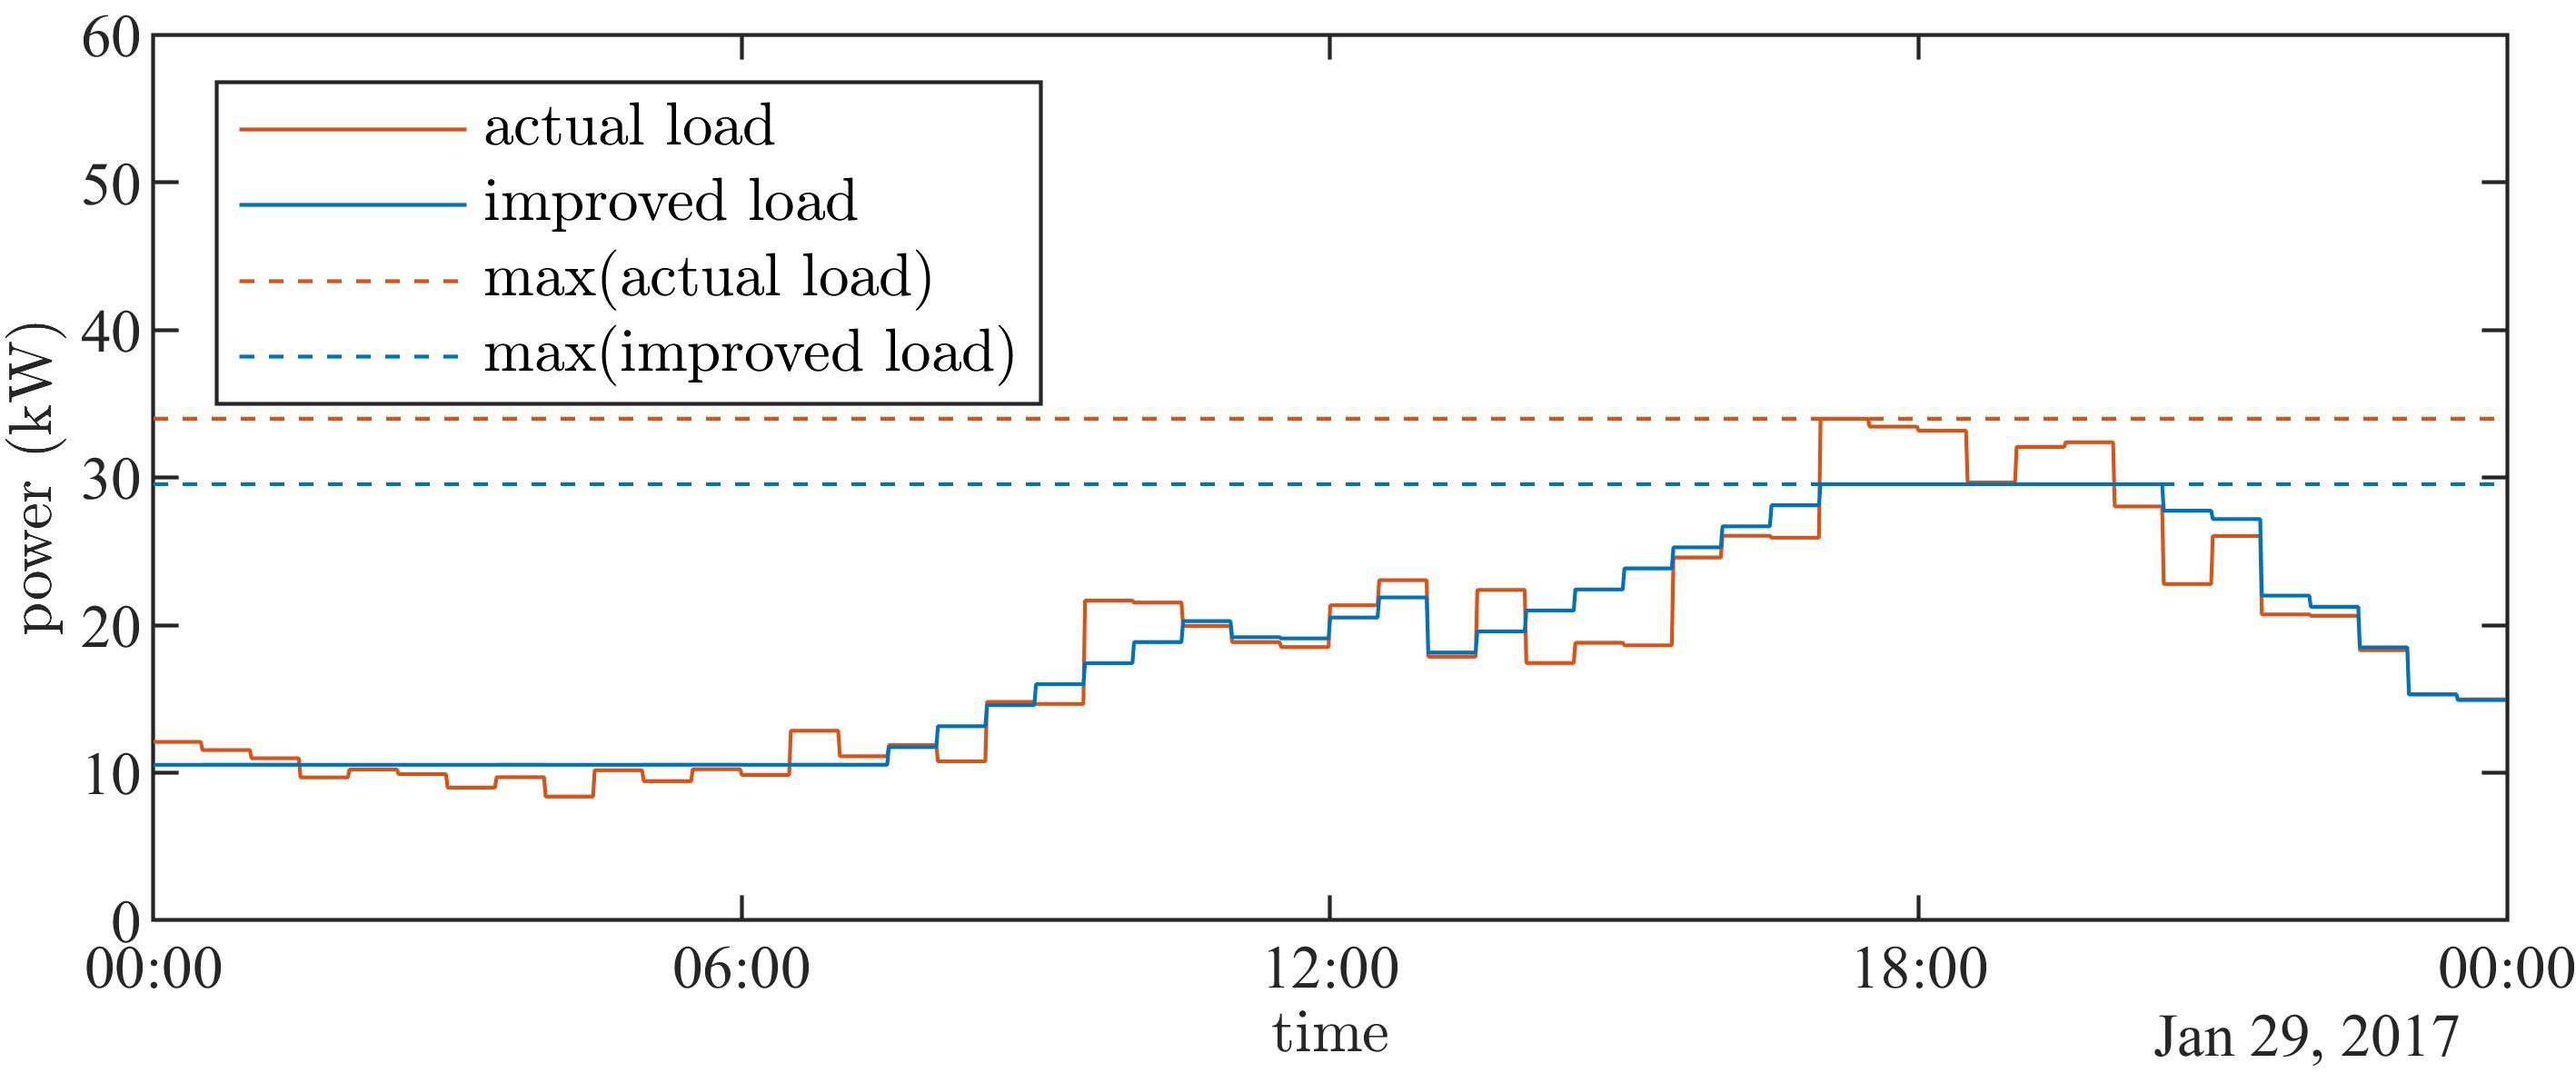
\includegraphics{_chapter2/fig/day-forecasted}
		\label{ch2:subfig:day-forecasted}
	}\\
	\subfloat[]{%
		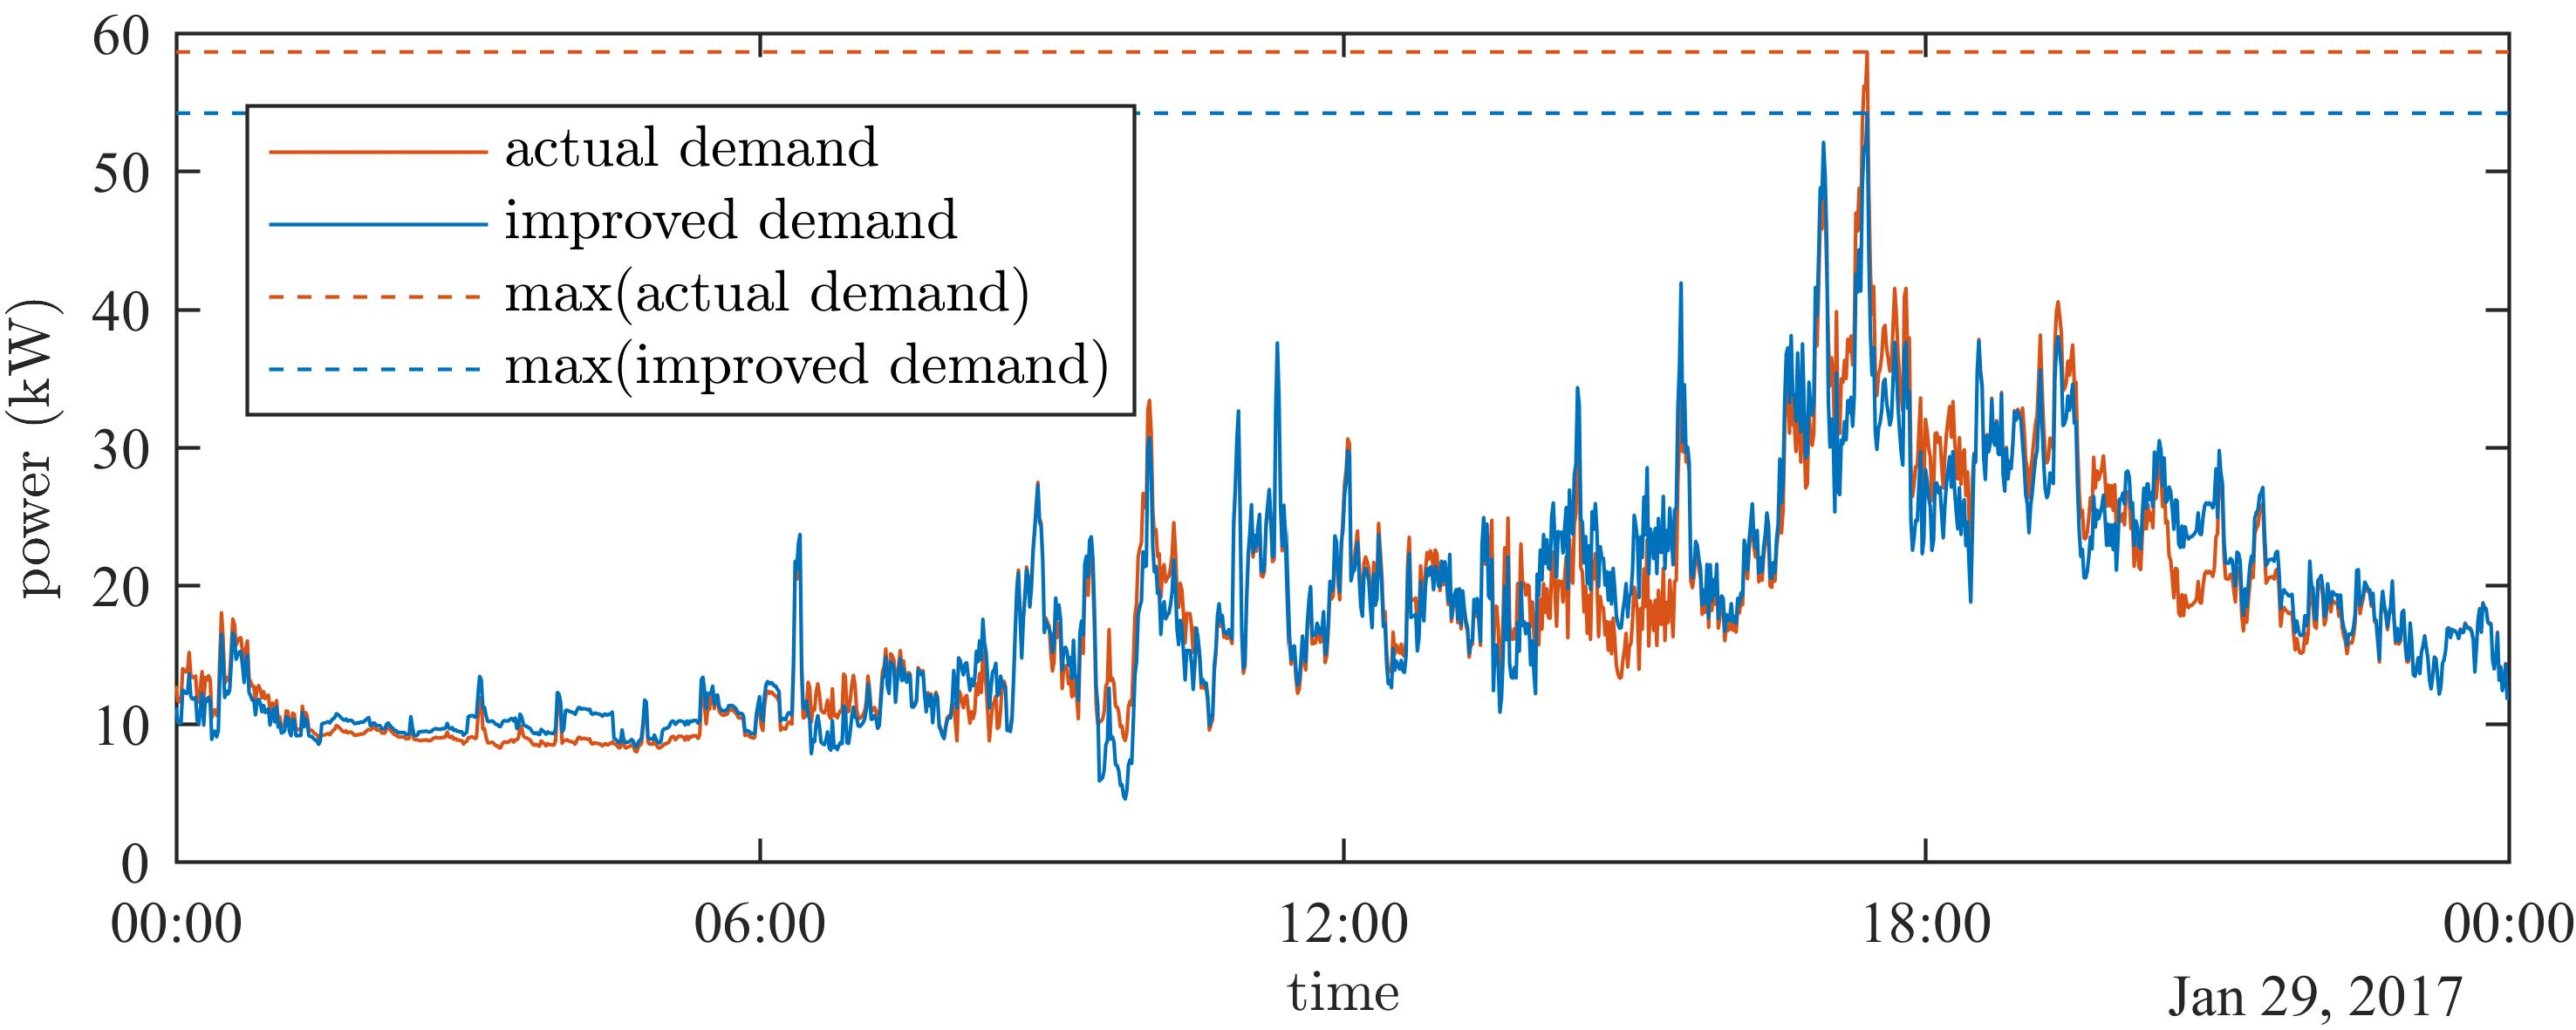
\includegraphics{_chapter2/fig/day-actual}
		\label{ch2:subfig:actual-forecasted}
	}
	\caption{An example of applying a half-hourly ESMU schedule to the half-hourly substation load (Subfig. \ref{ch2:subfig:day-forecasted}) and the actual, sub-half-hourly daily load, measured at the substation (Subfig. \ref{ch2:subfig:actual-forecasted}).}
	\label{ch2:fig:cost-sample}
\end{figure}

As repetitively mentioned, the ESMU operation that results from this scheduling mechanism is at half-hourly resolution and has therefore limited impact on sub-half-hourly load variation.
To visualise this limitation, a singe day's ESMU schedule was generated from its corresponding forecast as defined in Equation \ref{ch2:equ:cost-minimisation}, and plotted in Figure \ref{ch2:fig:cost-sample}.
In this simple comparison, the noticeable discrepancy between the half-hourly ESMU schedule and the actual, sub-half-hourly demand can be observed.
Furthermore, noticeable disparity in peak duration, magnitude and volatility can be noted.
This discrepancy and disparity emphasise the incompatibility issues between half-hourly ESMU schedules and the actual sub-half-hourly load.
As previously discussed, benefits of ESMU were intended to mitigate sub-half-hourly load volatility, yet this cannot be achieved when solely applying half-hourly ESMU schedules in an off-line manner.
Therefore, in the next section, the control strategy to add an on-line component is explained.




 

\section{Control of ESMU}
\label{ch2:sec:control-of-esmu}

\begin{figure}\centering
% Define some block styles
\tikzstyle{box} = [%
	draw,%
	rectangle,%
	%fill=green!20,%
	minimum height=3em,%
	minimum width=5em,%
]
\begin{tikzpicture}[node distance=2cm, shorten >= 1pt, >=stealth', auto, scale=0.8, transform shape]
	% Define nodes
    \path
    (0,0)
    node [box, minimum width=5cm, yshift=0mm](network) {Network}
    node [box, below of=network, yshift=0mm](battery) {Battery}
    node [box, fill=green!20, below left of=battery, yshift=-20mm, xshift=-10mm](pid_soc) {PID$_1$}
    node [box, fill=green!20, below right of=battery, yshift=-20mm, xshift=10mm](pid_p) {PID$_2$}
    node [box, fill=blue!20, below of=pid_soc, yshift=-15mm](schedule) {Schedule}
    node [box, fill=green!20, below of=pid_p, yshift=-15mm](mpc) {MPC};
	% Draw lines
	\draw [->] (battery) to (network);
	\draw [->, bend right] (pid_soc) to node[left, pos=0.4, xshift=-1mm] {$p_{1}(t+\Delta t)$} (battery);
	\draw [->, bend left] (pid_p) to node[right, pos=0.4, xshift=1mm] {$p_{2}(t+\Delta t)$} (battery);
	\draw [->] (battery.180) to [out=180, in=120] node[left, pos=0.2, xshift=-5mm] {$SOC^*(t)$} (pid_soc.180|-pid_soc.90);
	\draw [->] (network.0) to [out=340, in=60] node[left, pos=0.4] {$p_\text{net}(t)$} (pid_p.0|-pid_p.90);
	\draw [->] (schedule) to node[pos=0.25] {$SOC(t)$} (pid_soc);
	\draw [->] (mpc) to node[pos=0.25] {$\hat{p}_\text{net}(t+\Delta t)$} (pid_p);
	\draw [->, bend left] (network.0) to [out=80, in=100] node[right, pos=0.1, xshift=2mm, yshift=1mm] {$p_\text{net}(t)$} (mpc.0);
	
	\draw (-5, -6.75) node [right] {Controller};
	
	\draw [dashed] (-5, -3.5) -- (5, -3.5) -- (5, -6.5) -- (-5, -6.5) -- (-5, -3.5);
%	\draw [->, bend right] (schedule.180) to (controller.90);
%	\draw [->] (network) to (mpc);
%	\draw [->] (mpc) to (controller);
%	\draw [->] (controller) to (battery);
%	\draw [->] (battery) to (network);
\end{tikzpicture}%


\caption{Dynamic controller breakdown as previously shown in Figure \ref{ch2:subfig:proposed-dynamic-control-system}.}
\label{ch2:fig:system-controller}
\end{figure}


\hl{This section explains the dynamic control (i.e. the controller block as shown in Figure~}\ref{ch2:subfig:proposed-dynamic-control-system}\hl{) in the shape of an MPC, containing the two PID compensators to adjust operation around the predetermined ESMU schedule.}
The first PID compensator is fed by the ESMU schedule and the other is fed by the predictor load estimations.
After the control system is detailed in this section the auto-regressive models which were used during the course of this research are also explained.

\subsection{Dynamic control}

The content of the dynamic control procedure is shown in Figure~\ref{ch2:fig:system-controller}.
Here two reference signals are used as inputs to the dynamic control.
The first reference signal is the SOC profile derived from the ESMU scheduled, $SOC(t)$, and the second is an estimated future network power, $\hat{p}_\text{net}(t+\Delta t)$.
These two inputs are fed into compensator PID$_1$ and compensator PID$_2$, respectively.
The output of each compensator is a corrective battery power component that, when summed, yields the next ESMU power (i.e. $p_1(t+\Delta t)$ and $p_2(t+\Delta t)$) which is applied to the ESMU model.
Each PID compensator also receives a feedback signal to compute the internal error states.
More specifically, PID$_1$ receives the most recent SOC value that is obtained from the ESMU model, $SOC^*(t)$, and PID$_2$ receives the network's most recent power demand, $p_\text{net}(t)$ (for example through measurements by substation monitoring).

\nomenclature[J]{$p_\text{net}(t)$}{Most recent network demand at sample $t$, where $\textbf{p}_{net} = (p_\text{net}(t))$ and $p_\text{net}(t) \in \mathbb{R}$}
\nomenclature[J]{$SOC^*(t)$}{Battery's state of charge at sample $t$, where $SOC^*(t) \in [0, 1]$}
\nomenclature[J]{$E_\text{SOC}(t)$}{Error in state of charge at sample $t$, where $E_\text{SOC}(t) \in \mathbb{R}$}
\nomenclature[J]{$E_{p}(t)$}{Difference between current and predicting network power at sample $t$, where $E_{p}(t) \in \mathbb{R}$}
\nomenclature[J]{$\hat{p}_\text{net}(t+\Delta t)$}{Predicted next network power at sample $t$}
\nomenclature[J]{$\boldsymbol{\alpha}$}{PID weight vector for SOC compensator PID$_1$, where $\boldsymbol{\alpha} = \{\alpha_P, \alpha_I, \alpha_D\}$ and $\boldsymbol{\alpha} \in \mathbb{R}^3$}
\nomenclature[J]{$\boldsymbol{\beta}$}{PID weight vector for predictor compensator PID$_2$, where $\boldsymbol{\beta} = \{\beta_P, \beta_I, \beta_D\}$ and $\boldsymbol{\beta} \in \mathbb{R}^3$}
\nomenclature[J]{$\textbf{a}$}{Weight vector for compensator input regression of the AR model, where $\textbf{a} = \mathbb{R}^{N}$}
\nomenclature[J]{$\textbf{b}$}{Weight vector for compensator output regression of the AR model, where $\textbf{b} = \mathbb{R}^{N}$}
\nomenclature[J]{$N$}{Number of regressors of the AR model, where $N \in \mathbb{Z}_{>0}$}
\nomenclature[J]{$p_1(t)$}{Corrective ESMU power components from PID$_1$, where $p_1(t) \in \mathbb{R}$}
\nomenclature[J]{$p_2(t)$}{Corrective ESMU power components from PID$_2$, where $p_2(t) \in \mathbb{R}$}
\nomenclature[J]{$SOC_{tol}$}{SOC tolerance, i.e. maximum deviation from the prescheduled SOC profile, where $SOC_{tol} \in [0, 0.5]$}

Inside the PID$_1$ component a SOC error term, $E_\text{SOC}(t)$, is computed.
This term is the difference between the scheduled SOC profile, $SOC(t)$, and the actual (or simulated) SOC values, $SOC^*(t)$.
The following equation captures this error term.

\begin{equation}
	E_{SOC}(t) := SOC^*(t) - SOC(t)
	\label{ch2:equ:soc-error}
\end{equation}

Applying a standard and linearly weighted dynamic gain vector, $\boldsymbol{\alpha}$, to the SOC error allows the calculation of a corrective ESMU power component dynamically.
Here $\boldsymbol{\alpha} = \{\alpha_P, \alpha_I, \alpha_D\}$ and the components are the P, I and D weights, respectively.
How to determine the values of $\boldsymbol{\alpha}$ is explained later in this section.
This corrective power is denoted as $p_1(t+\Delta t)$, and is defined as follows:

\begin{equation}
\begin{split}
	p_1(t+\Delta t) &:= \alpha_P E_{SOC}(t)\\
	&+ \alpha_I \sum_{i=0}^\infty E_{SOC}(t-i\Delta t)\\
	&+ \alpha_D \frac{E_{SOC}(t)-E_{SOC}(t-\Delta t)}{\Delta t}
\end{split}
\label{ch2:equ:corrective-component-soc}
\end{equation}

Here the integral component removes steady-state error and the instantaneous error differential prevents overshooting.
All in all, this compensator uses present and past values to issue a corrective future ESMU instruction.
Compensator PID$_2$ on the other hand uses values from the present, past and future in order to minimise the power transient and load peaks.

\begin{figure}[htb]\centering
% Define some block styles
\tikzstyle{box} = [%
	draw,%
	rectangle,%
	%fill=green!20,%
	minimum height=3em,%
	minimum width=5em,%
]
\tikzstyle{sample} = [draw, circle, fill, scale=0.4]
\tikzstyle{estimate} = [draw, circle, solid, fill=white, scale=0.4]
\begin{tikzpicture}[node distance=2cm, shorten >= 1pt, >=stealth', auto, scale=0.9, transform shape]
	% Draw axis and labels
	\draw [<->] (0, 6) -- (0, 0) -- (12, 0);
	\draw (12, 0) node [anchor=north east] {Time};
	\draw (0, 3) node [anchor=south, rotate=90] {Power};
	% Add axis ticks
	\foreach[count=\i, evaluate=\i as \l using int(\i-1)] \t in {1,4,...,10}
	{
		\draw (\t,0.1) -- (\t,-0.1);
		\ifthenelse{\l=0}
		{\draw (\t,-0.1) node[anchor=north] {$t$}}
		{
			\ifthenelse{\l=1}
			{\draw (\t,-0.1) node[anchor=north] {$t+\tau$}}
			{\draw (\t,-0.1) node[anchor=north] {$t+\l\tau$}};
		};
	}
	% Draw main power curve
	\draw [thick]
	(0.5, 2.1) to
	(1, 2) node[sample](sam_0) {} to
	(4, 4) node[sample](sam_1) {} to
	(7, 3.5) node[sample](sam_2) {} to
	(10, 2) node[sample](sam_3) {} to
	(11, 1.8);
	
	% Add power sample forward projection
	\draw [dashed] (1, 2) -- (4.6, 2);
	\draw [dashed] (4, 4) -- (7.5, 4);
	\draw [dashed] (7, 3.5) -- (10.5, 3.5);
	\draw [dashed] (10, 2) -- (10.5, 2);
	
	% Plot estimates
	\draw [dotted] (1, 2) to
	(4, 3.7) node[estimate](est_1) {} to
	(7, 3.8) node[estimate](est_2) {} to
	(10,1.7) node[estimate](est_3) {};
	
	% Label the power samples
	\draw [->] (1, 5) node[anchor=south] {$p(t)$} to [out=-135,in=135] (sam_0);
	\draw [->] (4, 5) node[anchor=south] {$p(t+\tau)$} to [out=-135,in=135] (sam_1);
	\draw [->] (7, 5) node[anchor=south] {$p(t+2\tau)$} to [out=-135,in=135] (sam_2);
	\draw [->] (10, 5) node[anchor=south] {$p(t+3\tau)$} to [out=-135,in=135] (sam_3);
	
	% Label the estimates
	\draw [->] (4, 0.75) node[anchor=north] {$\hat{p}(t+\tau)$} to [in=-45] (est_1);
	\draw [->] (7, 0.75) node[anchor=north] {$\hat{p}(t+2\tau)$} to [in=-45] (est_2);
	\draw [->] (10, 0.75) node[anchor=north] {$\hat{p}(t+3\tau)$} to [in=-45] (est_3);
	
	% Label the forward power transients
	\draw [decorate,decoration={brace,amplitude=3pt,mirror,raise=4pt},yshift=0pt,xshift=5mm]
	(4, 2) -- (4, 4) node [anchor=west,black,midway,xshift=2mm] {$\epsilon_p(t)$};
	\draw [decorate,decoration={brace,amplitude=3pt,mirror,raise=4pt},yshift=0pt,xshift=3mm]
	(7, 3.5) -- (7, 4) node [anchor=west,black,midway,xshift=2mm] {$\epsilon_p(t+\tau)$};
	\draw [decorate,decoration={brace,amplitude=3pt,mirror,raise=4pt},yshift=0pt,xshift=3mm]
	(10, 2) -- (10, 3.5) node [anchor=west,black,midway,xshift=2mm] {$\epsilon_p(t+2\tau)$};
	
\end{tikzpicture}
%	\draw [solid] (12, 6) -- (12, 4.75) -- (10.5, 4.75) -- (10.5, 6) -- (12, 6);
%	\draw (10, 6) node[sample, yshift=-10mm, xshift=25mm](legend_sample) {};
%	\draw node[right of=legend_sample, xshift=-15mm] {$p$};
%	\draw (10, 6) node[estimate, yshift=-20mm, xshift=25mm](legend_estimate) {};
%	\draw node[right of=legend_estimate, xshift=-15mm] {$\hat{p}$};
\caption{Underlying time-series based compensation strategy for compensator PID$_2$. Here, $p_{network}$ and $\hat{p}_{network}$ are abbreviated to $p$ and $\hat{p}$, respectively.}
\label{ch2:fig:power-transient-minimisation}
\end{figure}


Figure~\ref{ch2:fig:power-transient-minimisation} summarises the time series computations for each power sample at times $t$, $t+\Delta t$, etc.
Ideally, PID$_2$ uses present power readings, $p_\text{net}(t)$, and a power value of the immediate future, i.e. $p_\text{net}(t+\Delta t)$, to compute a power error signal, which is to be reduced to a smallest possible value.
This error signal is defined as:

\begin{equation}
	E_p(t) := p_\text{net}(t+\Delta t) - p_\text{net}(t)
	\label{ch2:equ:power-error-signal}
\end{equation}

However, since the future network power is unknown an ``estimated next power'', $\hat{p}_\text{net}(t+\Delta t)$, is used instead.
This value is the PID$_2$'s input from the predictor and results in an ``estimated power error signal'':

\begin{equation}
	\hat{E}_{p}(t) = \hat{p}_{net}(t+\tau) - p_{net}(t)
	\label{ch2:equ:power-error-estimate}
\end{equation}

Similarly to PID$_1$, PID$_2$ produces a corrective ESMU power component, $p_2(t)$, that smoothens the resulting power profile.
This corrective ESMU power is also computed using a standard linear weighted dynamic vector $\boldsymbol{\beta}$, with $\boldsymbol{\beta} = \{\beta_P, \beta_I, \beta_D\}$, being the P, I and D weight, respectively:

\begin{equation}
\begin{split}
	p_2(t+\tau) &:= \beta_P E_{p}(t)\\
	&+ \beta_I \sum_{i=0}^\infty E_{p}(t-i\tau)\\
	&+ \beta_D \frac{E_{p}(t)-E_{p}(t-\tau)}{\tau}
\end{split}
\label{ch2:equ:corrective-component-power}
\end{equation}

Similar to $\boldsymbol{\alpha}$ how to determine the values of $\boldsymbol{\beta}$ is explained later in this section.
Finally, the ``next ESMU power'' can be deduced by adding the two corrective ESMU power components, as shown in the equation below.

\begin{equation}
	p(t+\Delta t) = p_1(t+\Delta t) + p_2(t+\Delta t)
	\label{ch2:equ:next-battery-power}
\end{equation}

Both PID compensators do however depend on correctly chosen weights for $\boldsymbol{\alpha}$ and $\boldsymbol{\beta}$.
Therefore they need to be tuned prior to executing the dynamic control.
For this work a minimisation problem was formulated that is based on a cost function, $\zeta^*(\boldsymbol{\alpha}, \boldsymbol{\beta})$, to deduce the two weight vectors as follows:

\begin{equation}
	\min_{\alpha,\beta} \zeta^*(\alpha, \beta) \text{ s.t. }
	\begin{cases}
		SOC(t) - SOC_{tol} \leq 0\\
		-SOC(t) \leq 0\\
		SOC(t) - 1 \leq 0
	\end{cases}
	\forall t
	\label{ch2:equ:cost-weights}
\end{equation}

Here, $\zeta^*(\boldsymbol{\alpha}, \boldsymbol{\beta})$ is defined as:

\begin{equation}
\begin{split}
	\zeta^*(\boldsymbol{\alpha}, \boldsymbol{\beta}) := \max_t(\textbf{p}_{net} + \textbf{p})\\
	\text{ where } \textbf{p}_{net} = (p_\text{net}(t)) \text{ and } \textbf{p} = (p(t))
\end{split}
\label{ch2:equ:dynamic-cost}
\end{equation}

In Equation~\ref{ch2:equ:cost-weights} and Equation~\ref{ch2:equ:dynamic-cost}, $\zeta^*(\boldsymbol{\alpha}, \boldsymbol{\beta})$ represents the sub-half-hourly peak load during a day when ESMU schedules are adjusted with the corresponding $\boldsymbol{\alpha}$ and $\boldsymbol{\beta}$ weights.
Also, the same SOC tolerance that was used to generate the SOC schedule (i.e. $SOC_{tol}$) is included to prevent the solution from deviating off the prescheduled SOC profile.
To generalise this solution for all load cases this minimisation problem was formulated to solve multiple daily load profiles in order to find ideal values for $\boldsymbol{\alpha}$ and $\boldsymbol{\beta}$.
\hl{The system of two PID compensators for discrete time is unconventional and it is worth considering different types of control or compensator.
However, with the above-explained approach and for the data used as part of this research, the computed set of $\boldsymbol{\alpha}$ and $\boldsymbol{\beta}$ weights resulted a convergent and stable solutions.
In this context, convergent means that the $SOC^*(t)$ values tend towards the $SOC(t)$ values, and stable means that the $SOC^*(t)$ values never clipped at zero or one.
The details concerning these case studies themselves are however outlined in Section~}\ref{ch2:sec:case-studies}\hl{.}

\subsection{Model predictive control}

As explained in the literature review in Chapter~\ref{ch-literature}, Model Predictive Control (MPC) is favoured over Set-Point Control (SPC), since it takes into account time-series to produce a behaviour.
With this knowledge, MPC can be used to not only react to recent changes but also to counteract foreseen trends.
Different approaches exist to obtain these foreseen trends and these approaches highly vary in accuracy, computational burden and robustness.
Equally, the characteristics of underlying data which is used to train these models impacts their performances.
For the presented work in this chapter, an efficient and robust approach is required since potential ESMU deployment with SSEN demands these functional requirements.
Prediction accuracy on the other hand is an optional requirement which becomes important only when the predicting model can issue predictions in real-time and does (for the predicting horizon) remain stationary and bounded.

The simplest form of producing a prediction is to assume that the currently observed trending load will also occur in the future.
This kind of prediction does however not take into account demand dynamics.
%Instead, it uses the mean power which is explained as follows:
%
%\begin{equation}
	\hat{p}(t+\Delta t) = \frac{1}{N}\sum_{i=0}^{N-1}p(t-i\Delta t)
	\label{ch2:equ:simple-prediction}
\end{equation}
%
%Here, the estimated next power, $\hat{p}(t+\Delta t)$, is derived as the average past powers, $p(t)$, over an averaging horizon, $N$.
An AR model on the other hand uses a series of past observations and their individual contribution to predict the next power.
But the further into the future these predictions are made the less accurate they become.
This accuracy loss is however circumvented since the hybrid system was designed to only apply corrections based on load predictions of the immediate future (i.e. next sample time at $t+\Delta t$ and not $t+2\Delta t$ or similar).
This simplification also reduces computational burden and guarantees real-time operation especially when choosing the simplest dynamic model (i.e. an Auto-Regressive (AR) model instead of deep artificial neural networks).
Since external forces can and often do impact the behaviour of the model, the AR model is treated as an exogenous model with a time-series of input powers, $\textbf{p} = (p(t))$, a time-series of predicted ``next powers'', $\hat{\textbf{p}} = (\hat{p}(t))$, and an internal delay function $t-\Delta t$.

\begin{figure}\centering
% Define some block styles
\tikzstyle{box} = [%
	draw,%
	rectangle,%
	%fill=green!20,%
	minimum height=2em,%
	minimum width=2em,%
]
\begin{tikzpicture}[node distance=2cm, shorten >= 1pt, >=stealth', auto, scale=0.9, transform shape]
	\pgfmathsetmacro\N{4}

	% Draw input nodes
    \draw
    (0, 0) node [](input) {$p(t)$}
    (1, 0) node [](input_1) {};
    % Draw output nodes
    \draw
    (6.5, 0) node [](output) {$\hat{p}(t+\Delta t)$}
    (5, 0) node [](output_1) {};
    % Draw main adder node
    \draw (3, 0) node [circle, draw](adder_main) {+};
    % Link input, adder and output
    \draw [->] (input) to (adder_main);
    \draw [->] (adder_main) to (output);
    % Draw AR model nodes
    \foreach[count=\i, evaluate=\i as \l using int(\i*2)] \n in {1,2,...,\N}
	{
		\ifthenelse{\n<\N}
		{
	    	\draw (1, 1-\l) node [box](z_a\n) {$z^{-1}$};
	    	\draw (1, -\l) node [](half_a\n) {};
	    	\draw (1.8, -\l) node [box](a\n) {$a_\n$};
	    	
	    	\draw (5, 1-\l) node [box](z_b\n) {$z^{-1}$};
	    	\draw (5, -\l) node [](half_b\n) {};
	    	\draw (4.2, -\l) node [box](b\n) {$b_\n$};
	    	
	    	\draw (3, -\l) node [circle, draw](adder_\n) {+};
    	}{
	    	\draw (1, 1.95-\l) node [](z_a\n) {};
	    	\draw (5, 1.95-\l) node [](z_b\n) {};
    	}
    	\ifthenelse{\n=1}
    	{
    		\draw [->] (input_1.center) to (z_a\n);
    		\draw [->] (output_1.center) to (z_b\n);
    		\draw [->] (adder_\n) to (adder_main);
    	}{
    		\pgfmathtruncatemacro{\dn}{\n-1};
    		\pgfmathtruncatemacro{\dnn}{\n-2};
    		\ifthenelse{\n<\N}
			{
				\ifthenelse{\dn=1}
				{
					\draw [->] (z_a\dn) to node[left]{$p(t-\Delta t)$} (z_a\n);
				}{
					\draw [->] (z_a\dn) to node[left]{$p(t-\dn\Delta t)$} (z_a\n);
				}
				\ifthenelse{\dnn=0}
				{
					\draw [->] (z_b\dn) to node[right]{$\hat{p}(t)$} (z_b\n);
				}{
					\ifthenelse{\dnn=1}
					{
						\draw [->] (z_b\dn) to node[right]{$\hat{p}(t-\Delta t)$} (z_b\n);
					}{
						\draw [->] (z_b\dn) to node[right]{$\hat{p}(t-\dnn\Delta t)$} (z_b\n);
					}
				}
				\draw [->] (adder_\n) to (adder_\dn);
			}{
				\draw [-] (z_a\dn) to node[left]{$p(t-\dn\Delta t)$} (z_a\n.center);
				\draw [-] (z_b\dn) to node[right]{$\hat{p}(t-\dnn\Delta t)$} (z_b\n.center);
			}
    		\draw [->] (half_a\dn.center) to (a\dn);
    		\draw [->] (a\dn) to (adder_\dn);
    		\draw [->] (half_b\dn.center) to (b\dn);
    		\draw [->] (b\dn) to (adder_\dn);
    	}
    }

\end{tikzpicture}
\caption{Exogenous auto-regressive model that is used for model predictive control. Here, $z^{-1}$ indicates the time delay by one sample period, i.e. $\Delta t$.}
\label{ch2:fig:mpc-arx}
\end{figure}


Figure~\ref{ch2:fig:mpc-arx} graphically captures the standard AR model's function tree which is equivalently represented mathematically in the following equation:

\begin{equation}
\begin{split}
	\hat{p}(t+\Delta t) &= p(t) + \sum_{i=1}^{N} a_i p(t-i\Delta t)\\
	&+ \sum_{i=1}^{N} b_i \hat{p}(t-(i-1)\Delta t)
\end{split}
\label{ch2:equ:mpc-arx}
\end{equation}

Values of the two weight vectors $\textbf{a}$ and $\textbf{b}$, where $\textbf{a} = (a_i)$ and $\textbf{b} = (b_i)$, are determined during runtime using the standard adaptive least squares algorithm, i.e.:

\begin{equation}
	\min_{\textbf{a}, \textbf{b}} \left(p(t) - \hat{p}(t)\right)^2
\label{ch2:equ:least-squares-1}
\end{equation}
Or:
\begin{equation}
	\min_{\textbf{a}, \textbf{b}} \left(p(t) - p(t - \Delta t) + \sum_{i=2}^{N} a_i p(t-i\Delta t) + \sum_{i=2}^{N} b_i \hat{p}(t-(i-1)\Delta t)\right)^2
\label{ch2:equ:least-squares-2}
\end{equation}


Therefore, the proposed algorithm adjusts $\textbf{a}$ and $\textbf{b}$ to minimise the prediction error at each time-step.
Beside finding optimised values for $\textbf{a}$ and $\textbf{b}$, the model's number of regressors, $N$, is also expected to impact the model's performance ($N$ is also referred to as the ``model length'').
The example in Figure~\ref{ch2:fig:mpc-arx} represents a symmetric model where $N=3$.
This short length however is most likely insufficient in predicting $p(t+\Delta t)$ which is why several models of increasing lengths are assessed and compared in the results section of this chapter.
From this comparison the impact of $N$ on the models' resulting values of $\hat{p}(t+\Delta t)$ and correspondingly on the performance of the dynamic controller can be determined and discussed.
Details about the cases for different model length are presented in the case studies in Section~\ref{ch2:sec:case-studies}.


\section{Case studies}
\label{ch2:sec:case-studies}

Two cases are defined that the performance of the proposed dynamic control is compared against: case \textbf{O} and case \textbf{B}.
More specifically, case \textbf{O}, original case, is the scenario where no BESS operation takes place.
Traditional off-line BESS operation that only uses predetermined half-hourly BESS schedules is referred to as the benchmark case, or case \textbf{B}.
All remaining cases, which are explained below, are capture different versions of the dynamic control.

In addition to the two comparison cases, three more different case studies are defined: cases \textbf{I}, \textbf{II} and \textbf{III}.
This group of three case studies evaluates the impact of the proposed dynamic control when subjected to realistic (i.e. imperfect) half-hourly load forecasts.
In each of the three cases, a different mechanisms is used to predict the power volatility.
More specifically:
\begin{itemize}
	\item case \textbf{I} implements the simplest prediction mechanism, i.e. it is assumed that the current power measurements repeats,
	\item case \textbf{II} uses the aforementioned MPC, and performance of different AR model lengths is compared, and
	\item case \textbf{III},the third and final case, represents an ideal scenario where perfect foresight is assumed and the exact next load can be estimated.
\end{itemize}
For clarity, all three cases, numbered \textbf{I} to \textbf{III}, are summarised and tabulated in Table \ref{ch2:tab:cases}.

\begin{table}[htb]\centering
	\begin{tabular}{r | c c}
		& real forecast & ideal forecast\\
		\hline
		repeated power estimation & \textbf{I} & \textbf{IV}\\
		MPC power estimation & \textbf{II} & \textbf{V}\\
		perfect power foresight & \textbf{III} & \textbf{VI}\\
	\end{tabular}
	\caption{Six cases and their dynamic control input assumptions}
	\label{ch2:tab:cases}	
\end{table}

Results from all BESS cases (\textbf{B}, \textbf{I}, \textbf{II} and \textbf{III}) are first compared against the original, i.e. uncompensated, network load case (\textbf{O}).
Here, by using a sample day, the assessment of load profile improvements are made clear.
Once it is clear how each day's peak is reduced by the algorithm, the daily peak reduction capability from all cases' results are compared.
Rather than assessing the underlying load profile from a time-series perspective, only focus is put on any further peak load reductions.
However, the number of days may make it difficult to spot trends and improvements in the data.
Therefore, from the daily peak reduction results, a Probability Density Function (PDF) is derived, which is based on kernel density estimation.
The PDF shows the stochastic improvement of each case type in comparison to the original case, i.e. case \textbf{O}.


\section{Results and Discussion}
\label{ch1:sec:results-and-discussion}


\section{Conclusion}
\label{ch2:sec:conclusion}

\chapter{Effects of Desynchronising Information Propagation when Distributing Smart-Charging}
\label{ch3}

\section{Overview}
\label{ch3:sec:overview}

In previous chapters the the question regarding how one can optimally control a single battery energy storage has been addressed.
It was shown that half-hourly forecasts can be used to predict demand due to customer behaviours.
With this knowledge, Battery Energy Storage Systems (BESS) can be scheduled to shave peak load in order to avoid overloading the already stressed system.
But sub-half-hourly issues could not be addressed by traditional BESS schedules, which is why two successive sub-half-hourly power adjustment methods were developed.
The first method improved network operation by focusing on the underlying three-phase network topology, whilst strictly following the underlying half-hourly SOC plan.
The second method on the other hand alleviated this constraint by adjusting total power flow instead.
Benefits from using BESS schedules complement dynamic feedback and yield improved power profiles with reduced peak load.

The next step is to take such schedules and apply them to multiple, distributed batteries.
To prevent the negative impact from battery charging, particularly when dealing with the home-charging of Electric Vehicles (EVs), their charging scheduling needs to be coordinated.
As already discussed in the literature review in Chapter \ref{ch-literature}, multiple control methods to coordinate Distributed Energy Resources (DER) that including EV charge scheduling methods, exist \cite{Atia2016, Bidram2012, Bidram2014, Dolan2012, Gill2014, Guerrero2008, Guerrero2013, Sugihara2013, Toledo2013, Wang2016, Vovos2007, Guerrero2013a, Mansouri-Samani1993, Marra2013, Mokhtari2013}. 
Those approaches propose demand prioritisation, multi-tariff environments and even other game theory based methods to maximise utility or to reduce cost.
In the context of EV charging, coordination their charge scheduling signals becomes a vital requirement to react to other EV's charging plans.
This statement is commonly acknowledged since most smart charging research focuses on algorithm improvements, but in a distributed system this scheduling assumption of perfect knowledge exchange no longer holds.

In fact, during distributed EV scheduling, control instructions that may be broadcasted by one EV to inform all other EVs in the system of e.g. an updated charging plan, need not or cannot be received and responded to at the exact same times unless some synchronisation amongst all EVs is guaranteed.
Therefore, this chapter assesses the impact of desynchronising message propagation by adding transmission jitter to the updating broadcasts, since the effect on the performance of a traditionally synchronised EV scheduling algorithm is unknown, and by doing so this chapter addresses objective 3 of this thesis, this was outlined in Section \ref{ch-introduction:sec:problem-statement}.
The charging of EVs is explicitly assessed instead of managing a collection of BESSs, since storage is able to release energy and thus provide grid support.
Traditional EVs on the other hand do not have such capabilities and need to be coordinated in order to avoid home-charging related load spikes.
To achieve this coordination, a robust smart-charging algorithm to determine multiple EVs' charging schedule is presented and executed in both a synchronised and a desynchronised messaging scenario.
A Multi-Agent System (MAS) is implemented to perform the distributed scheduling using the Foundation for Intelligent Physical Agents (FIPA) compliant agents.

Results show how synchronised scheduling leads to expected outcomes that have also been established in literature.
However, adding jitter to message broadcasting significantly changes the same algorithm's behaviour.
Differences regarding rate of convergence and criteria for stability are most noticeable.
The structure of this chapter is as follows:
First, the EV demand and scheduling mechanism to coordinate the synchronised and desynchronised smart-charging is explained in Section \ref{ch3:sec:ev-coordination}.
Next, in Section \ref{ch3:sec:distributed-systems}, the distributed control system for the chosen MAS is presented, alongside the two cases for synchronised and desynchronised information propagation.
Section \ref{ch3:sec:results} presents and discusses the results from these two cases, upon which a conclusion is drawn in Section \ref{ch3:sec:summary}.


\section{Coordination of EV charging}
\label{ch3:sec:ev-coordination}

In this section, an algorithm for EV charging is presented, which is later implemented in both a synchronised and desynchronised case.
Real load data is used in combination with EV demand to evaluate the performance of the algorithm at preventing new power spikes from occurring.
Convergence of the algorithm is studied and convergence criteria as well as rate of convergence are presented, too.

The structure of this section is as follows.
First, the means and assumptions for calculating EV demand is defined.
Then the real load data is introduced and explained.
The EV scheduling algorithm is introduced next, before the performance parameters are presented.

\subsection{EV Demand}

\nomenclature[K]{$T_\text{sch}$}{Scheduling horizon for EV charging, where $T_\text{sch} \in \mathbb{Z}^{>0}$ (Chapter \ref{ch3})}
\nomenclature[K]{$u$}{EV unit number, where $u \in [1, \dots, U]$ (Chapter \ref{ch3})}
\nomenclature[K]{$n$}{Iteration number of EV scheduling algorithm, where $N \in [1, \dots, N]$ (Chapter \ref{ch3})}
\nomenclature[K]{$U$}{Number of EVs that need to be scheduled, where $U \in \mathbb{Z}^{>0}$ (Chapter \ref{ch3})}
\nomenclature[K]{$N$}{Number of algorithm iterations to schedule multiple EVs, where $N \in \mathbb{Z}^{>0}$ (Chapter \ref{ch3})}
\nomenclature[K]{$p_{\text{EV},u,n}(t)$}{Scheduled EV charging power, for EV $u$ at algorithm iteration $n$ for time $t$, where $p_{\text{EV},u,n}(t) \in \mathbb{R}^{\geq 0}$ (Chapter \ref{ch3})}
\nomenclature[K]{$\textbf{p}_{\text{EV}, u, n}$}{Scheduled EV charging power vector, for EV $u$ at algorithm iteration $n$, where $p_{\text{EV},u,n}(t) \in \textbf{p}_{\text{EV},u,n}$ (Chapter \ref{ch3})}

\nomenclature[K]{$P_{\text{min},u}$}{Minimum EV charging power (Chapter \ref{ch3})}
\nomenclature[K]{$P_{\text{min},u}$}{Maximum EV charging power (Chapter \ref{ch3})}

EVs were modelled as loads that, over the course of a scheduling horizon, $T_\text{sch}$, each need to consume a certain amount of energy, $E_u$, to simulate charging their batteries.
Each EV, i.e. $u$, is part of a fleet of charging and coordinated EVs, i.e. $u \in [1, \dots, U]$.
Unlike typical loads (e.g. households), EVs do not have a predetermined load profile in this simulation and are therefore flexible to schedule their demand at each time $t$ a $p_{\text{EV},u,n}(t)$, where $p_{\text{EV},u,n}(t) \in \textbf{p}_{\text{EV},u,n}$.
In other words, they can autonomously assign their own charging plan over the predetermined number of future time-slots, $T_\text{sch}$.
Due to limitations in on-board power electronics, each EV's maximum charge rate, $P_{\text{max},u}$, is restricted and may not be exceeded.
Equally, in order to meet the EV's charging demand over the scheduling horizon, $T_\text{sch}$, a soft minimum charging power, $P_{\text{min},u}$ is also introduced:

\begin{equation}
	P_{min,u} := \frac{E_u}{H}
	\label{ch3:equ:power-charge-minimum}
\end{equation}

Although the upper limit is hard, i.e. caused by technical restrictions, this lower limit is a necessity to initiate the scheduling procedure, which will become apparent when the scheduling algorithm is explained.
Using MAS, EVs utilise their broker agents to purchase energy quantities for each time-slot, $t$, and also sell or ``undo'' some of the already acquired energy quantities if it contributed towards a new load spike.

\subsection{Base Load}

\nomenclature[K]{$\Delta t$}{Sample period for EV scheduling, where $\Delta t \in \mathbb{R}^{>0}$ (Chapter \ref{ch3})}

To represent real power consumption in simulations, historic customer load profiles were used in this work \cite{IrishData2002}.
This dataset consisted of 7392 demand readings for 543 loads, which were sampled at half-hourly period, i.e. $\Delta t = 0.5$ hours.
A single scheduling horizon was defined as one day, therefore $T_\text{sch}=48$ samples.

In this context, each household, i.e. physical entity, dispatches its broker agents to order the household's daily energy demand; therefore it a scenario with some foresight is assumed.
After having issued this energy request, the entire network demand is known to the supplier and can be relayed to all broker agents when they query for it.
This ability is exploited when scheduling and negotiating the unknown EV charging profiles.
More specifically, all households' broker agents communicate with the suppler's broker agents to optimally embed their charging profiles, $p_{\text{EV},u,n}(t)$, within this aggregated base load.

\subsection{Scheduling Algorithm}

For the EV charging coordination strategy, an algorithm was designed that generates optimised charging profiles for each EV.
Here, optimality implies that when adding all aggregated charging profiles to the network's base demand, $p_\text{base}(t)$, no additional spikes occur in the resulting demand profile, i.e. $p_\text{base}(t) + \sum_{u=1}^U p_{EV,u,N}(t)$.
These profiles were generated by repetitively querying for the network's base load, adjusting individual EV charging profiles, and resubmitting the adjusted charging profile.
As already stated, the common assumption when designing such a scheduling algorithm is that all scheduling entities are synchronised, i.e. wait for each other, before querying for the network's base load.
For visualisation, the message exchange bewteen two loads and a supplier including a synchronisation time is shown in Figure \ref{ch3:fig:agent-synchronisation}.

\begin{figure}\centering
\tikzstyle{box} = [%
	draw,%
	rectangle,%
	%fill=green!20,%
	minimum height=2em,%
	minimum width=2em,%
]
\tikzstyle{bracket} = [%
	decorate,%
	decoration={brace,amplitude=5pt,raise=1mm},%
	yshift=0mm,%
	color=black!50,%
]
\tikzstyle{bracket_text} = [%
	black,%
	midway,%
	xshift=2mm,%
	align=left,%
	color=black!50,%
]
\begin{tikzpicture}[node distance=2cm, shorten >= 1pt, >=stealth', auto, scale=1, transform shape]
	\pgfmathsetmacro\N{4}

	% Draw supplyer
    \draw (0, 0) node [box, fill=black!10](supplier) {Supplier};
    \draw (5, 0) node [box, fill=black!10](load1) {Load$_1$};
    \draw (10, 0) node [box, fill=black!10](load2) {Load$_2$};
    
    \draw (0, -11.5) node [](s_end) {};
    \draw (0, -10) node [](s_sync) {};
    
    \draw (5, -1) node [](l1_q1) {};
    \draw (5, -2) node [](l1_r1) {};
    \draw (5, -5) node [](l1_u1) {};
    \draw (5, -6) node [](l1_a1) {};
    \draw (5, -11) node[](l1_q2) {};
    
    \draw (10, -1.1) node [](l2_q1) {};
    \draw (10, -3.0) node [](l2_r1) {};
    \draw (10, -7.5) node [](l2_u1) {};
    \draw (10, -8.5) node [](l2_a1) {};
    \draw (10, -11.1) node[](l2_q2) {};
    
    
    \draw [dotted] (supplier.south) to (s_end.center);
    \draw [dotted] (load1.south) to (s_end.center-|l1_q1.center);
    \draw [dotted] (load2.south) to (s_end.center-|l2_q1.center);
    
    \draw [->] (l1_q1.center) to node[pos=0.5, above]{query$(l_1)$} (supplier.center|-l1_q1);
    \draw [->] (supplier.center|-l1_q1) to
    			(supplier.center|-l1_r1) to node[pos=0.5, above]{reply$(l_1)$} (l1_r1.center);
    \draw [bracket] (l1_q1) -- (l1_r1) node[bracket_text]{waiting};
    \draw [->] (l1_r1.center) to 
    			(l1_u1.center) to node[pos=0.5, above]{update$(l_1)$} (supplier.center|-l1_u1);
    \draw [bracket] (l1_r1) -- (l1_u1) node[bracket_text]{scheduling};
    \draw [->] (supplier.center|-l1_u1) to
    			(supplier.center|-l1_a1) to node[pos=0.5, above]{ack$(l_1)$} (l1_a1.center);
    \draw [bracket] (l1_u1) -- (l1_a1) node[bracket_text]{waiting};
    \draw [bracket] (l1_a1) -- (l1_a1|-s_sync.90) node[bracket_text]{syncing};
    
    \draw [->] (l2_q1.center) to node[pos=0.25, above]{query$(l_2)$} (supplier.center|-l2_q1);
    \draw [->] (supplier.center|-l2_q1) to
    			(supplier.center|-l2_r1) to node[pos=0.75, above]{reply$(l_2)$} (l2_r1.center);
    \draw [bracket] (l2_q1) -- (l2_r1) node[bracket_text]{waiting};
    \draw [->] (l2_r1.center) to
    			(l2_u1.center) to node[pos=0.25, above]{update$(l_2)$} (supplier.center|-l2_u1);
    \draw [bracket] (l2_r1) -- (l2_u1) node[bracket_text]{scheduling};
    \draw [->] (supplier.center|-l2_u1) to
    			(supplier.center|-l2_a1) to node[pos=0.75, above]{ack$(l_2)$} (l2_a1.center);
    \draw [bracket] (l2_u1) -- (l2_a1) node[bracket_text]{waiting};
    \draw [bracket] (l2_a1) -- (l2_a1|-s_sync.90) node[bracket_text]{syncing};
    
    \draw [thick] (supplier.180|-s_sync) to node[pos=1, right]{SYNC} (load2.0|-s_sync);
    
    \draw [->] (l1_q2.center) to node[pos=0.5, above]{query$(l_1)$} (supplier.center|-l1_q2);
    \draw [->] (l2_q2.center) to node[pos=0.25, above]{query$(l_2)$} (supplier.center|-l2_q2);
    
    \draw [-] (supplier.center|-l1_q2) to (s_end.center);
\end{tikzpicture}	
\caption{Agent synchronisation before re-scheduling their EVs charging profile.}
\label{ch3:fig:agent-synchronisation}
\end{figure}

In this figure, the horizontal arrows indicate messages being sent from loads (i.e. EV agents) to a supplier and vertical lines indicate processing or idle time.
Shown within Figure \ref{ch3:fig:agent-synchronisation} is a single scheduling iteration, which can be broken into the sub-processes of: querying, scheduling, updating and synchronising.
From top to bottom, the sequential execution of these sub-processes is as follows:

First, both load$_1$ and load$_2$ query the supplier for the currently known network load (i.e. query($l_1$) and query($l_2$)).
This network load is used to schedule their power profiles to ``fill valleys'', i.e. only charge EVs during periods of low demand.
Upon receipt of a reply from the energy supplier (i.e. reply($l_1$) and reply($l_2$)), both loads immediately start scheduling their profiles.
In the example above, load$_1$ found a solution before load$_2$ and can therefore inform the supplier about its intended load profile sooner, by sending an update (i.e. update$(l_1)$) to the supplier.
Subsequently querying the supplier for an updated network load would be premature, since the other load (i.e. load$_2$) has not yet generated and updated its load profile.
Therefore, a synchronisation mechanism had to be used, forcing load$_1$ to wait until all loads have sent updates to the supplier.
Here, load$_1$ waits until load$_2$ has sent an update and the corresponding profile was acknowledged by the supplier (i.e. ack$(l_2)$).
Only after this had happened, a synchronisation event would be triggered (i.e. \textit{SYNC} event).
After this synchronisation event, the next algorithm iteration is initiated and the procedure repeats.
Since all subsequent iterations are similar to the one shown in Figure \ref{ch3:fig:agent-synchronisation}, only the two querying messages of the  second iteration are shown.

Although the timing and message exchange has been defined, the mechanism to allocate and reallocate charging powers in order to achieve a valley filling behaviour has not yet been defined.
This behaviour is shown in Figure \ref{ch3:fig:valley-filling}, where several iterations numbered $n$ are shown, and for each subsequent iteration, some amount of prescheduled power is reallocated to different time-slots.

\begin{figure}\centering
\subfloat[]{%
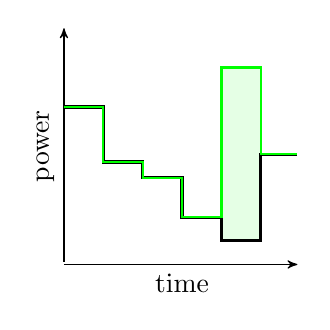
\begin{tikzpicture}[node distance=2cm, shorten >= 1pt, >=stealth', auto, scale=1, transform shape]
	\draw [<-] (0, 3) to node[pos=0.5,rotate=90,anchor=south]{power} (0, 0);
	\draw [->] (0, 0) to node[pos=0.5,anchor=north]{time} (3, 0);
	\draw (2.25, 0.3) node [fill=green!10,minimum width=0.5cm,minimum height=2.2cm,anchor=south](rect_add) {};
	\draw [very thick]
	(0.0, 2.0) -- (0.5, 2.0) --
	(0.5, 1.3) -- (1.0, 1.3) --
	(1.0, 1.1) -- (1.5, 1.1) --
	(1.5, 0.6) -- (2.0, 0.6) --
	(2.0, 0.3) -- (2.5, 0.3) --
	(2.5, 1.4) -- (3.0, 1.4);
	\draw [thick, green]
	(0.0, 2.0) -- (0.5, 2.0) --
	(0.5, 1.3) -- (1.0, 1.3) --
	(1.0, 1.1) -- (1.5, 1.1) --
	(1.5, 0.6) -- (2.0, 0.6) --
	(2.0, 2.5) -- (2.5, 2.5) --
	(2.5, 1.4) -- (3.0, 1.4);
\end{tikzpicture}%
\label{ch3:subfig:valley-filling-1}%
}
\hspace{10mm}
\subfloat[]{%
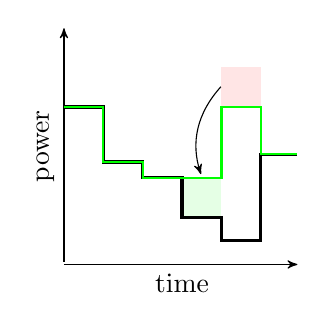
\begin{tikzpicture}[node distance=2cm, shorten >= 1pt, >=stealth', auto, scale=1, transform shape]
	\draw [<-] (0, 3) to node[pos=0.5,rotate=90,anchor=south]{power} (0, 0);
	\draw [->] (0, 0) to node[pos=0.5,anchor=north]{time} (3, 0);
	\draw (2.25, 2.0) node [fill=red!10,minimum width=0.5cm,minimum height=0.5cm,anchor=south](rect_sub) {};
	\draw (1.75, 0.6) node [fill=green!10,minimum width=0.5cm,minimum height=0.5cm,anchor=south](rect_add) {};
	\draw [very thick]
	(0.0, 2.0) -- (0.5, 2.0) --
	(0.5, 1.3) -- (1.0, 1.3) --
	(1.0, 1.1) -- (1.5, 1.1) --
	(1.5, 0.6) -- (2.0, 0.6) --
	(2.0, 0.3) -- (2.5, 0.3) --
	(2.5, 1.4) -- (3.0, 1.4);
	\draw [thick, green]
	(0.0, 2.0) -- (0.5, 2.0) --
	(0.5, 1.3) -- (1.0, 1.3) --
	(1.0, 1.1) -- (1.5, 1.1) --
	(1.5, 1.1) -- (2.0, 1.1) --
	(2.0, 2.0) -- (2.5, 2.0) --
	(2.5, 1.4) -- (3.0, 1.4);
	\draw [->, bend right] (rect_sub.180) to (rect_add.90);
\end{tikzpicture}%
\label{ch3:subfig:valley-filling-2}%
}
\hspace{10mm}
\subfloat[]{%
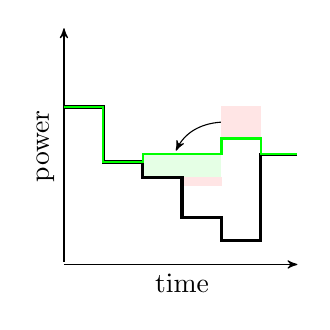
\begin{tikzpicture}[node distance=2cm, shorten >= 1pt, >=stealth', auto, scale=1, transform shape]
	\draw [<-] (0, 3) to node[pos=0.5,rotate=90,anchor=south]{power} (0, 0);
	\draw [->] (0, 0) to node[pos=0.5,anchor=north]{time} (3, 0);
	\draw (2.25, 1.6) node [fill=red!10,minimum width=0.5cm,minimum height=0.4cm,anchor=south](rect_sub_1) {};
	\draw (1.75, 1.0) node [fill=green!10,minimum width=0.5cm,minimum height=0.4cm,anchor=south](rect_add_1) {};
	\draw (1.25, 1.1) node [fill=green!10,minimum width=0.5cm,minimum height=0.3cm,anchor=south](rect_add_2) {};
	\draw [fill=red!10,red!10] (1.5, 1.0) rectangle (2.0,1.1);
	\draw [very thick]
	(0.0, 2.0) -- (0.5, 2.0) --
	(0.5, 1.3) -- (1.0, 1.3) --
	(1.0, 1.1) -- (1.5, 1.1) --
	(1.5, 0.6) -- (2.0, 0.6) --
	(2.0, 0.3) -- (2.5, 0.3) --
	(2.5, 1.4) -- (3.0, 1.4);
	\draw [thick, green]
	(0.0, 2.0) -- (0.5, 2.0) --
	(0.5, 1.3) -- (1.0, 1.3) --
	(1.0, 1.4) -- (1.5, 1.4) --
	(1.5, 1.4) -- (2.0, 1.4) --
	(2.0, 1.6) -- (2.5, 1.6) --
	(2.5, 1.4) -- (3.0, 1.4);
	\draw [->, bend right] (rect_sub_1.180) to (rect_add_2.45);
\end{tikzpicture}%
\label{ch3:subfig:valley-filling-3}%
}
\vspace{1mm}
\subfloat[]{%
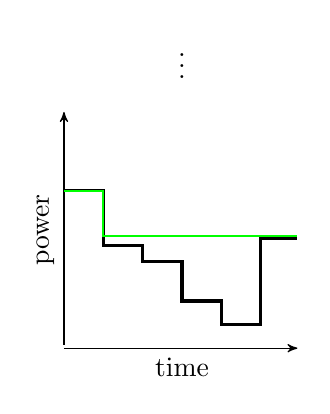
\begin{tikzpicture}[node distance=2cm, shorten >= 1pt, >=stealth', auto, scale=1, transform shape]
	\draw [<-] (0, 3) to node[pos=0.5,rotate=90,anchor=south]{power} (0, 0);
	\draw [->] (0, 0) to node[pos=0.5,anchor=north]{time} (3, 0);
	\draw [very thick]
	(0.0, 2.0) -- (0.5, 2.0) --
	(0.5, 1.3) -- (1.0, 1.3) --
	(1.0, 1.1) -- (1.5, 1.1) --
	(1.5, 0.6) -- (2.0, 0.6) --
	(2.0, 0.3) -- (2.5, 0.3) --
	(2.5, 1.4) -- (3.0, 1.4);
	\draw [thick, green]
	(0.0, 2.0) -- (0.5, 2.0) --
	(0.5, 1.42) -- (1.0, 1.42) --
	(1.0, 1.42) -- (1.5, 1.42) --
	(1.5, 1.42) -- (2.0, 1.42) --
	(2.0, 1.42) -- (2.5, 1.42) --
	(2.5, 1.42) -- (3.0, 1.42);
	\draw (1.5, 3.3) node[anchor=south] {$\vdots$};
\end{tikzpicture}%
\label{ch3:subfig:valley-filling-4}%
}
\caption{Charging power allocation for valley-filling behaviour}
\label{ch3:fig:valley-filling}	
\end{figure}

\nomenclature[K]{$p_{\text{base},n}(t)$}{Base load at time $t$, where $p_{\text{base},n}(t) \in \mathbb{Z}^{\geq0}$ (Chapter \ref{ch3})}
\nomenclature[K]{$\textbf{p}_{\text{base},n}$}{Base load vector, where $p_{\text{base},n}(t) \in \textbf{p}_{\text{base},n}$ (Chapter \ref{ch3})}
\nomenclature[K]{$\hat{p}_{\text{base},n}(t)$}{Temporary demand at time $t$, i.e. the aggregate of all EV charge vector and the base load vector, where $\hat{p}_{\text{base},n}(t) \in \mathbb{Z}^{\geq0}$ (Chapter \ref{ch3})}
\nomenclature[K]{$\hat{\textbf{p}}_{\text{base},n}$}{Temporary demand vector, i.e. the aggregate of all EV charge vector and the base load vector, where $\hat{p}_{\text{base},n}(t) \in \hat{\textbf{p}}_{\text{base},n}$ (Chapter \ref{ch3})}

For every iteration in Figure \ref{ch3:fig:valley-filling}, charging profiles are added onto a base network load, $\textbf{p}_{base,n}$, where $p_{base,n}(t) \in \textbf{p}_{base,n}$.
This base load is shown as the bold black line and does not change throughout EV scheduling.
For any iteration, the charging profile during iteration number $n$, for EV $u$, is defined as $\textbf{p}_n$ (where $p_{u,n}(t) \in \textbf{p}_n$).
During the first iteration however, i.e. Figure \ref{ch3:subfig:valley-filling-1} where $n=1$, this charging profile is determined by assigning the maximum EV charging power to the time-slots of lowest load, until the total EV energy demand is met, i.e. at time-slot $\tau$ where $\tau = \text{argmin}(\textbf{p}_\text{base})$.
Since all EVs schedule their profiles based upon the same knowledge of $\textbf{p}_{base,n}$, the aggregated charging power is likely to generate a new spike.
This spike is seen on an updated or temporary demand profile, $\hat{\textbf{p}}_{\text{base}, n}$, where $\hat{p}_{\text{base}, n}(t) \in \hat{\textbf{p}}_{\text{base}, n}$ is defined as:

\begin{equation}
	\hat{p}^\text{base}_{n}(t) := p^\text{base}_{n}(t) + \sum_{u=1}^{U} p_{u,n}(t) \forall t, n
	\label{ch3:equ:updated-demand-profile}
\end{equation}

\nomenclature[K]{$\hat{p}_{\text{EV}, u, n}(t)$}{Temporary charging power during iteration number $n$, for EV $u$, at time $t$, where $\hat{p}_{\text{EV}, u, n}(t) \in \textbf{Z}^{\geq0}$ (Chapter \ref{ch3})}
\nomenclature[K]{$\hat{\textbf{p}}_{\text{EV}, u, n}$}{Temporary charging vector during iteration number $n$, for EV $u$, where $\hat{p}_{\text{EV}, u, n}(t) \in \hat{\textbf{p}}_{\text{EV}, u, n}$ (Chapter \ref{ch3})}

For the next iteration $n+1$, i.e. Figure \ref{ch3:subfig:valley-filling-2} where $n=2$, a proportion of the previously scheduled power vector $\textbf{p}_{\text{EV},n-1}$ is ``undone''.
Subsequently, the spike in the resulting $\hat{\textbf{p}}_{\text{base}, n}$ is reduced, yet the energy that has been undone needs to be reallocated.
The amount by which $\textbf{p}_{\text{EV},n-1}$ is reduced is determined by the ``\textit{undoing}'' parameter $\alpha$, where $\alpha \in [0, 1)$.
A new reduced or temporary charging vector $\hat{p}_{\text{EV}, u, n}(t)$ is therefore defined as:

\begin{equation}
	\hat{p}^\text{EV}_{u,n}(t) := p^\text{EV}_{u,n-1}(t)(1-\alpha)
	\label{ch3:equ:temporary-charging-power}
\end{equation}

Using this temporary charging power, the regained or temporary energy demand, $\hat{E}_{u,n}$, that needs to be reallocated, can also be defined:

\begin{equation}
	\hat{E}_{u,n} := E_u - \sum_{\tau=1}^{T_\text{sch}} \hat{p}_{\text{EV},u,n}(\tau)\Delta t \forall u \text{ and } n > 1
	\label{ch3:equ:temporary-charging-demand}
\end{equation}

To include the first iteration of the algorithm, Equation \ref{ch3:equ:temporary-charging-demand} needs to be expanded to redefine $\hat{E}_{u,n}$ for all possible algorithm iterations $n$:

\begin{equation}
	\hat{E}_{u,n} :=
	\begin{cases}
		E_u &\text{if } n=1\\
		E_u - \sum_{\tau=1}^{T_\text{sch}} \hat{p}_{\text{EV},u,n}(\tau)\Delta t &\text{otherwise}
	\end{cases}
	\forall u \text{ and } \forall n
	\label{ch3:equ:temporary-charging-demand-expanded}
\end{equation}

Following the similar procedure as for the first iteration, $\hat{E}_{u,n}$ needs to be allocated to different time-slots, where the rule of performing the power allocation is defined as:

\begin{equation}
\begin{split}
	p_{u,k}(n) :=
	\begin{cases}
		\frac{\hat{E}_u(n)}{\kappa}\beta &\text{if } \frac{\hat{E}_u(n)}{\kappa}\beta \leq P_{max,u}\\
		P_{max,i} &\text{otherwise}
 	\end{cases}
 	\forall u  \\\text{ where } k = \text{argmin}_k(\textbf{p}_{base}(n)) \text{ and } n > 1
\end{split}
\label{ch3:equ:valley-filling-equation}
\end{equation}

\nomenclature[K]{$\beta$}{Allocation parameter to assign a portion of the temporary energy demand, $\hat{E}_{u,n}$, where $\beta \in (0, 1]$ (Chapter \ref{ch3})}

Here, a maximum ``allocation'' parameter, $\beta$, where $\beta \in (0, 1]$ limits the power that may be allocated to any successive time-slot, $\tau$.
To not exceed the EV's maximum charging power, any value in the charging vector, $\textbf{p}_{\text{EV},u,n}$, is capped to $P_{\text{max},u}$.
If $\beta$ is chosen as one, then the undone energy is allocated as quickly as possible.
For smaller values of $\beta$ on the other hand, the undone charge is reallocated in smaller portions.
Since EV scheduling takes place over a finite scheduling horizon, $T_\text{sch}$, a constraint was added in Equation \ref{ch3:equ:valley-filling-equation}.
This was done to assure that the temporary energy demand equates after some charging power was assigned to every time-slot of $\textbf{p}_{\text{EV},u,n}$.

Any following algorithm iteration, i.e. $n>2$ as shown in Figure \ref{ch3:subfig:valley-filling-3}, the entire charging profile is adjusted and spread further over the base load, $\textbf{p}_\text{base}$.
In the end, i.e. when $n=N$, the ideal EV charging profiles aggregate with the base load in such a way, that the resulting network load has an optimally filled valley.
This valley filling behaviour is achieved with the ``undoing'' and ``allocation'' of EV charging power from one algorithm iteration to the next.
Regardless of the final network load's shape, the algorithm terminates when the final iteration is reached, i.e. $n=N$.
Rate of convergence of the algorithm differs based upon the choice of $\alpha$ and $\beta$ values.
However, convergence is in fact guaranteed when selecting values of $\alpha < 1$ and $\beta < 1$, since the algorithm satisfies the D'Alembert Criterion in those cases.

To summarise this section, the complete EV scheduling algorithm was developed by: 
\begin{enumerate*}
	\item defining the message exchange and synchronisation mechanism, which is shown in Figure \ref{ch3:fig:agent-synchronisation};
	\item formulating the initial and successive ``undoing'' of charging power, as shown in Equation \ref{ch3:equ:temporary-charging-power}; and
	\item defining the iterative update and ``allocation'' of the temporary energy demand, as defined in Equation \ref{ch3:equ:temporary-charging-demand-expanded}.
\end{enumerate*}
For clarity, the this smart charging algorithm's pseudocode, performing the complete valley filling procedure, has been included in Algorithm \ref{ch3:alg:valley-filling}.

\begin{algorithm}
 \SetKwFunction{Query}{query}
 \SetKwFunction{Update}{update}
 \SetKwFunction{Break}{break}
 \SetKwFunction{Sync}{synchronising}
 \KwData{$\textbf{p}_{\text{base},n}$, $E_u$, $P_{\text{max},u}$, $P_{\text{min},u}$, $\Delta t$, $T_\text{sch}$}
 \KwResult{$\textbf{p}_{\text{EV},u,n}$}
 \For{$n\leftarrow 1$ \KwTo $N$}{
  \tcp{Query for base load}\label{cmt}
  $\textbf{p}_{\text{base},n} \leftarrow$ \Query{}\;
  \tcp{Forward and undo previous schedule}\label{cmt}
  \eIf{$n>1$}{
    $\textbf{p}_{\text{EV},u,n} \leftarrow \textbf{p}_{\text{EV},u,n-1}\alpha$\;
   }{
    $\textbf{p}_{\text{EV},u,n} \leftarrow [0, 0, \dots, 0]$\;
  }
  \tcp{Determine unallocated energy}\label{cmt}
  $\hat{E}_{u,n} = E_u - \sum_{\tau=1}^{T_\text{sch}} p_{\text{EV},u,n}(\tau)\Delta t$\;
  \tcp{Fill valley}\label{cmt}
  \For{$\tau\leftarrow \text{argmin}(\textbf{p}_{\text{base},n})$ \KwTo $\text{argmax}(\textbf{p}_{\text{base},n})$}{
   \eIf{$p_{\text{EV},u,n}(\tau) + \frac{\hat{E}_{u,n}}{\Delta t}\beta \leq P_{\text{max},u}$}{
    $p_{\text{EV},u,n}(\tau) \leftarrow p_{\text{EV},u,n}(\tau) + \frac{\hat{E}_{u,n}}{\Delta t}\beta$\;
   }{
    $p_{\text{EV},u,n}(\tau) \leftarrow P_{\text{max},u}$\;
   }
   $\hat{E}_{u,n} = E_u - \sum_{\tau=1}^{T_\text{sch}} p_{\text{EV},u,n}(\tau) \Delta t$\;
   \tcp{Once EV profile is found, send update}\label{cmt}
   \If{$\hat{E}_{u,n} = 0$}{
    \Update{$\textbf{p}_{\text{EV},u,n}$}\;
   	\Break{}\;
   }
  }
  \Sync{}\;
 }
 \caption{Robust valley filling algorithm for a single EV in}
 \label{ch3:alg:valley-filling}
\end{algorithm}















\section{Distributed Systems}
\label{ch3:sec:distributed-systems}

As discussed in the literature review in Chapter \ref{ch-literature}, several mechanisms exist to decentralise control of DERs.
For their reactivity, pro-activeness, social ability and flexibility however, the Multi Agent System (MAS) distinguished itself from traditional software and hardware systems, which is why it was also chosen for the coordination of smart EV charging.
Several agent package implementations exist, each following different interaction paradigms.
Some of these paradigms include ``Belief, Desire and Intention'' (BDI), neutral behaviour or other specialised functionality \cite{Luck2004}.
From the catalogue of MAS paradigms, the Java Agent Development Framework (JADE) was chosen, since it natively implements the Foundation for Intelligent Physical Agent (FIPA) specification \cite{JADE-website, FIPA-agent-specs}.
Furthermore, JADE is an application independent package that has become quite popular, as seen by the increasing number of publications \cite{Karfopoulos2013, Eddy2011, Kuo2013, Mocci2014, Li2017}.

In this work, multiple virtual trading agents are used to negotiate their corresponding EV charging profile with other trading agents.
Tying virtual agents to a physical entity is not new \cite{Dimeas2005, Nguyen2011, Nagata2011, Nagata2012}, and allows a clear decoupling of the data storing and interacting entities.
In previous work however, physical agents directly controlled the virtual entities whilst the agents in the presented work negotiate schedules that will be applied after schedule ratification.
Therefore, the physical agent is never notified of any intermediate charging profile and only receives the final schedule.
Scheduling and inter-agent communication is achieved by so called ``broker'' agents that follow the Brokering Interaction Protocol (BIP) to serve the final charging profile when requested.
It is those broker agents that communicate and negotiate with each other by following the Contact-Net Protocol (CNP).
All these FIPA protocols are based on the FIPA Agent Communication Language (ACL) that is required to communicate over a shared telecommunications infrastructure since it standardises the communication ontology and schemas.
Following this standard also opens the possibility of including different agent packages into the scheduling mechanism, but this lies outside the work's scope.
Explanations of all protocols that were used in this implementation of FIPA agents are included in Appendix \ref{appx-b:multi-agent-systems}.
In this work, each broker is linked to a single EV and negotiates its charging profile over the aforementioned scheduling horizon, $T_\text{sch}$.
This link is shown in Figure~\ref{ch3:fig:agent-network}.

\begin{figure}\centering
\tikzstyle{box} = [%
	draw,%
	rectangle,%
	%fill=green!20,%
	minimum height=2em,%
	minimum width=2em,%
]
\begin{tikzpicture}[node distance=2cm, shorten >= 1pt, >=stealth', auto, scale=1, transform shape]
	\pgfmathsetmacro\N{4}

	% Draw supplyer
    \draw
    (0, 0)
    node [box, fill=black!10](supplier) {Supplier}
    node [box, below left of=supplier](buyer_s) {Buyer}
    node [box, below right of=supplier](seller_s) {Seller};
    
    \draw (5, 0) node(bracket) {};
    
    \draw
    node [box, below of=buyer_s, yshift=-10mm](buyer_1) {Buyer}
    node [box, below left of=buyer_1, fill=black!10](load_1) {Load}
    node [box, above left of=load_1](seller_1) {Seller}
    node [box, below of=seller_s, yshift=-10mm](seller_2) {Seller}
    node [box, below right of=seller_2, fill=black!10](load_2) {Load}
    node [box, above right of=load_2](buyer_2) {Buyer};
    
    \draw [-] (supplier) to (buyer_s);
    \draw [-] (supplier) to (seller_s);
    \draw [-] (load_1) to (buyer_1);
    \draw [-] (load_1) to (seller_1);
    \draw [-] (load_2) to (buyer_2);
    \draw [-] (load_2) to (seller_2);
    
    \draw [->] (seller_s) to node[pos=0.7, align=center, left, xshift=-5mm]{buys\\from} (buyer_1);
    \draw [->] (seller_s) to node[pos=0.7, align=center, right, xshift=5mm]{buys\\from} (buyer_2);
    \draw [->] (seller_1) to node[pos=0.3, align=center, left, xshift=-5mm]{sells\\to} (buyer_s);
    \draw [->] (seller_2) to node[pos=0.3, align=center, right, xshift=5mm]{sells\\to} (buyer_s);
    
	
    \draw [decorate,decoration={brace,amplitude=5pt,raise=0pt},yshift=0pt](supplier.90-|bracket.0) -- (supplier.270-|bracket.0) node [black,midway,xshift=2mm,align=left] {physical entity};
    \draw [decorate,decoration={brace,amplitude=5pt,raise=0pt},yshift=0pt](seller_s.90-|bracket.0) -- (seller_s.270-|bracket.0) node [black,midway,xshift=2mm,align=left] {CNP responding\\broker agents};
    \draw [decorate,decoration={brace,amplitude=5pt,raise=0pt},yshift=0pt](seller_2.90-|bracket.0) -- (seller_2.270-|bracket.0) node [black,midway,xshift=2mm,align=left] {CNP initiating\\broker agents};
    \draw [decorate,decoration={brace,amplitude=5pt,raise=0pt},yshift=0pt](load_2.90-|bracket.0) -- (load_2.270-|bracket.0) node [black,midway,xshift=2mm,align=left] {physical entities};
    
\end{tikzpicture}
\caption{A simplified MAS structure containing virtual seller and buyer agents (white), that negotiate power/charging profiles for physical entities (grey).}
\label{ch3:fig:agent-network}
\end{figure}

The example in Figure~\ref{ch3:fig:agent-network} shows the structure of a MAS with three physical agents and six virtual agents.
A supplier and two loads are the physical agents and two charging EVS, respectively, which dispatch two brokers each.
One of the brokers is for buying energy, i.e. ``allocating'' energy, and the other one for selling energy, i.e. ``undoing'' energy.
With this kind of system architecture, the scheduling algorithm can be executed to mitigate potential charging spikes.

How this MAS is implemented, synchronised and desynchronised is explained in the following sections, Section~\ref{ch3:subsec:implementation} and Section~\ref{ch3:subsec:desynchronisation}, respectively.
Subsequently, in Section~\ref{ch3:subsec:cases-and-metrics}, all case studies and performance metrics that are used to assess the MAS performance are outlined.

\subsection{MAS Implementation}
\label{ch3:subsec:implementation}

The MAS is implemented in Java and runs on a parallel compute cluster (i.e. the \textit{HTCondor} cluster at the former \textit{School of Systems Engineering} at the \textit{University of Reading}).
How the compute cluster was used to realise multiple agents is shown in Figure~\ref{ch3:fig:agent-implementation}.

\begin{figure}\centering
\tikzstyle{box} = [%
	draw,%
	rectangle,%
	%fill=green!20,%
	minimum height=2em,%
	minimum width=2em,%
]
\begin{tikzpicture}[node distance=2cm, shorten >= 1pt, >=stealth', auto, scale=1, transform shape]
	\draw (0, 0) node [box](biffo) {lab PC};
	\draw (5, 0) node [box, align=center](master) {\textit{HTCondor}\\submit node};
	\draw (10, 0) node [box](data) {data store};
	
	\draw (10, -5) node [box](supplier) {supplier};
	\draw node[above right of=supplier, yshift=-7.5mm] {\textit{worker$_5$}};
	
	\draw [->, line width=0.2mm, dotted] (biffo) to node[]{launch} (master);
	\draw [->, line width=0.2mm] (data) to node[pos=0.25, align=left, align=right, left]{network\\load} (supplier);
	
	\foreach[count=\i] \x in {0,3,...,10}
	{
		\draw (\x, -6.5) node [box](ev_\i) {EV};
		\draw node[below left of=ev_\i, yshift=7.5mm, xshift=5mm] {\textit{worker$_\i$}};
		\draw [<->, line width=0.4mm, bend right] (supplier) to (ev_\i);
		\draw [->, line width=0.2mm, dotted] (master) to (ev_\i);
	}
	
%	\draw [line, dashed] node (0, -2) -- node (10, -2);
	

%	\foreach[count=\i, evaluate=\i as \l using int(\i-1)] \t in {1,4,...,10}
%	{
%		\draw (\t,0.1) -- (\t,-0.1);
%		\ifthenelse{\l=0}
%		{\draw (\t,-0.1) node[anchor=north] {$t$}}
%		{
%			\ifthenelse{\l=1}
%			{\draw (\t,-0.1) node[anchor=north] {$t+\Delta t$}}
%			{\draw (\t,-0.1) node[anchor=north] {$t+\l\Delta t$}};
%		};
%	}

%	\pgfmathsetmacro\N{4}
%
%	% Draw supplyer
%    \draw
%    (0, 0)
%    node [box, fill=black!10](supplier) {Supplier}
%    node [box, below left of=supplier](buyer_s) {Buyer}
%    node [box, below right of=supplier](seller_s) {Seller};
%    
%    \draw (5, 0) node(bracket) {};
%    
%    \draw
%    node [box, below of=buyer_s, yshift=-10mm](buyer_1) {Buyer}
%    node [box, below left of=buyer_1, fill=black!10](load_1) {Load}
%    node [box, above left of=load_1](seller_1) {Seller}
%    node [box, below of=seller_s, yshift=-10mm](seller_2) {Seller}
%    node [box, below right of=seller_2, fill=black!10](load_2) {Load}
%    node [box, above right of=load_2](buyer_2) {Buyer};
%    
%    \draw [-] (supplier) to (buyer_s);
%    \draw [-] (supplier) to (seller_s);
%    \draw [-] (load_1) to (buyer_1);
%    \draw [-] (load_1) to (seller_1);
%    \draw [-] (load_2) to (buyer_2);
%    \draw [-] (load_2) to (seller_2);
%    
%    \draw [->] (seller_s) to node[pos=0.7, align=center, left, xshift=-5mm]{buys\\from} (buyer_1);
%    \draw [->] (seller_s) to node[pos=0.7, align=center, right, xshift=5mm]{buys\\from} (buyer_2);
%    \draw [->] (seller_1) to node[pos=0.3, align=center, left, xshift=-5mm]{sells\\to} (buyer_s);
%    \draw [->] (seller_2) to node[pos=0.3, align=center, right, xshift=5mm]{sells\\to} (buyer_s);
%    
%	
%    \draw [decorate,decoration={brace,amplitude=5pt,raise=0pt},yshift=0pt](supplier.90-|bracket.0) -- (supplier.270-|bracket.0) node [black,midway,xshift=2mm,align=left] {physical entity};
%    \draw [decorate,decoration={brace,amplitude=5pt,raise=0pt},yshift=0pt](seller_s.90-|bracket.0) -- (seller_s.270-|bracket.0) node [black,midway,xshift=2mm,align=left] {CNP responding\\broker agents};
%    \draw [decorate,decoration={brace,amplitude=5pt,raise=0pt},yshift=0pt](seller_2.90-|bracket.0) -- (seller_2.270-|bracket.0) node [black,midway,xshift=2mm,align=left] {CNP initiating\\broker agents};
%    \draw [decorate,decoration={brace,amplitude=5pt,raise=0pt},yshift=0pt](load_2.90-|bracket.0) -- (load_2.270-|bracket.0) node [black,midway,xshift=2mm,align=left] {physical entities};
    
\end{tikzpicture}
\caption{The implementation of FIPA on \textit{HTCondor}.}
\label{ch3:fig:agent-implementation}
\end{figure}

In this figure, Figure~\ref{ch3:fig:agent-implementation}, at the laboratory workstation, a collection of MAS simulations is compiled in order to extensively cover the algorithm's operating spectrum.
More specifically, 10000 repetitions of the scheduling algorithm are queued for a single base load, but with different $\alpha$ and $\beta$ parameters.
Therefore, the algorithm's parameter sensitivity is probed at a resolution of 0.01 for both $\alpha$ and $\beta$, i.e. $\alpha \in \{0.01, 0.02, \dots, 1.00\}$ and $\beta \in \{0.01, 0.02, \dots, 1.00\}$.
This queue of 10000 simulations is then submitted to the \textit{HTCondor} master node, which schedules the execution of each simulation to its pool of workers.
Each worker internally simulates an instance of the MAS and stores its outputs to a fast networked storage, which also serves as the worker's data source
Given the 1540 load profiles from the Irish dataset and assuming a typical distribution network of 55 customers, a theoretical limit of $6.11\times10^{101}$ simulations would exist.
Due to the limited time and size of the available worker pool (ca. 200 workers), a total number of $1.5\times10^{7}$ MAS simulations is chosen to yield a sufficiently accurate estimate of the algorithm's performance.
For all submitted simulations a relatively high EV uptake of 20\% was chosen in order to maximise the effect of badly scheduled EV charging, and in order to give the algorithm a larger energy volume when adjusting the EV charging schedules.
Also, in the diagram in Figure~\ref{ch3:fig:agent-implementation}, all bold arrows indicate fast data transmissions (used to acquire and store the datasets that are used for each MAS simulation), solid arrow indicates the loading of simulation data, and the dotted arrows indicate the software messages to submit and launch the MAS simulations.

\subsection{MAS Desynchronisation}
\label{ch3:subsec:desynchronisation}

Originally, the smart-charging algorithm was intended to run in a synchronised MAS environment, as shown in Figure~\ref{ch3:fig:agent-synchronisation}.
However, when aiming to desynchronise this operation, two distinct ways exist:
Either, any idle state that is interrupted by the synchronising signal (which is shown in Figure~\ref{ch3:fig:agent-synchronisation}) is removed and agent execution continues immediately, or agents are launched with a random jitter and operate in an execution loop with a fixed time delay.
Although the first approach would result in the quickest simulation execution, it still would require a synchronised start since one agent would already finish all algorithm iterations by the time a second agent joins the MAS.
Therefore, only the second way yields a truly desynchronised agent execution that still guarantees that all agents partake in the scheduling process.
Furthermore, using this jitter and therefore extending the execution time of each simulation makes the algorithm compliant with the compute cluster's terms of usage, since it would otherwise threaten to overload \textit{HTCondor} at managing the submission and data transfer between all workers.

In order to implement the second way of desynchronising agents, each agent is equipped with its individual loop timer that regulates its execution behaviour.
All agents are launched in quick succession and immediately begin their enumeration and scheduling tasks.
Desynchronisation amongst all agents is then achieved by introducing a jitter to both the agents' loop timers and the period between successive agent launches.
The resulting MAS then consisted of a completely desynchronised collection of agents, i.e. none of the agent's loop execution is aligned or dependent on any other agent's loop execution.
An example of this desynchronisation mechanism is presented in Figure~\ref{ch3:fig:agent-desynchronisation}.

\begin{figure}\centering
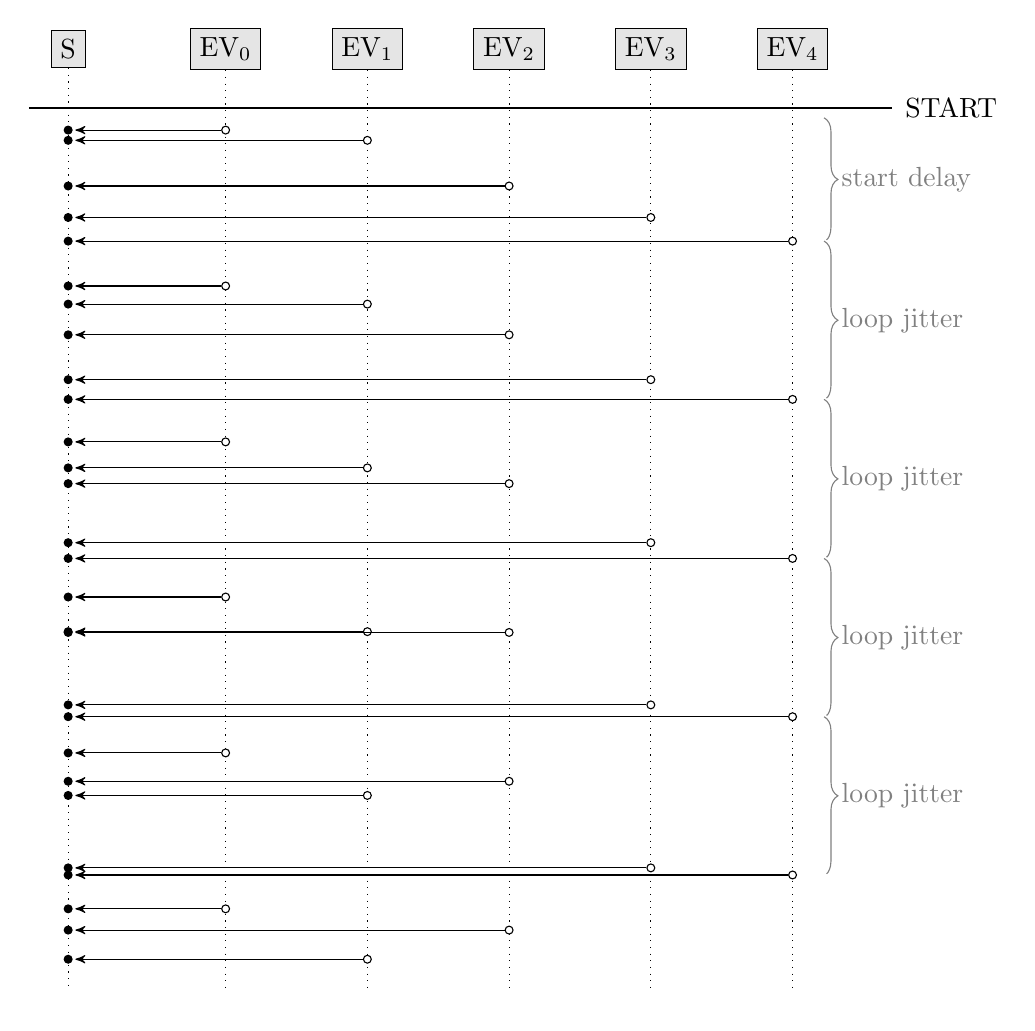
\begin{tikzpicture}[node distance=2cm, shorten >= 1pt, >=stealth', auto, scale=1, transform shape]

	\draw (0, 1) node [draw, rectangle, fill=black!10](supplier) {S};
	\draw [thick] (-0.5, 0.25) to node[pos=1, right]{START} (10.50, 0.25);
	\draw (0, -11.00) node [](s_end) {};
	\draw (9.50, 0.25) node [](legend) {};
	\draw [dotted] (supplier) -- (s_end-|supplier); 
	\draw (2.00, 1) node [draw, rectangle, fill=black!10](ev0) {EV$_0$};
	\draw [dotted] (ev0) -- (s_end-|ev0); 
	\draw (2.00,-0.03) node [draw, circle, inner sep=0pt, minimum size=1mm, fill=white](ev0y0) {};
	\draw (0,-0.03) node [draw, circle, inner sep=0pt, minimum size=1mm, fill=black](ss0y0) {};
	\draw [->] (ev0y0) to (ss0y0);
	\draw (2.00,-2.01) node [draw, circle, inner sep=0pt, minimum size=1mm, fill=white](ev0y1) {};
	\draw (0,-2.01) node [draw, circle, inner sep=0pt, minimum size=1mm, fill=black](ss0y1) {};
	\draw [->] (ev0y1) to (ss0y1);
	\draw (2.00,-3.99) node [draw, circle, inner sep=0pt, minimum size=1mm, fill=white](ev0y2) {};
	\draw (0,-3.99) node [draw, circle, inner sep=0pt, minimum size=1mm, fill=black](ss0y2) {};
	\draw [->] (ev0y2) to (ss0y2);
	\draw (2.00,-5.96) node [draw, circle, inner sep=0pt, minimum size=1mm, fill=white](ev0y3) {};
	\draw (0,-5.96) node [draw, circle, inner sep=0pt, minimum size=1mm, fill=black](ss0y3) {};
	\draw [->] (ev0y3) to (ss0y3);
	\draw (2.00,-7.94) node [draw, circle, inner sep=0pt, minimum size=1mm, fill=white](ev0y4) {};
	\draw (0,-7.94) node [draw, circle, inner sep=0pt, minimum size=1mm, fill=black](ss0y4) {};
	\draw [->] (ev0y4) to (ss0y4);
	\draw (2.00,-9.92) node [draw, circle, inner sep=0pt, minimum size=1mm, fill=white](ev0y5) {};
	\draw (0,-9.92) node [draw, circle, inner sep=0pt, minimum size=1mm, fill=black](ss0y5) {};
	\draw [->] (ev0y5) to (ss0y5);
	\draw (3.80, 1) node [draw, rectangle, fill=black!10](ev1) {EV$_1$};
	\draw [dotted] (ev1) -- (s_end-|ev1); 
	\draw (3.80,-0.16) node [draw, circle, inner sep=0pt, minimum size=1mm, fill=white](ev1y0) {};
	\draw (0,-0.16) node [draw, circle, inner sep=0pt, minimum size=1mm, fill=black](ss1y0) {};
	\draw [->] (ev1y0) to (ss1y0);
	\draw (3.80,-2.24) node [draw, circle, inner sep=0pt, minimum size=1mm, fill=white](ev1y1) {};
	\draw (0,-2.24) node [draw, circle, inner sep=0pt, minimum size=1mm, fill=black](ss1y1) {};
	\draw [->] (ev1y1) to (ss1y1);
	\draw (3.80,-4.32) node [draw, circle, inner sep=0pt, minimum size=1mm, fill=white](ev1y2) {};
	\draw (0,-4.32) node [draw, circle, inner sep=0pt, minimum size=1mm, fill=black](ss1y2) {};
	\draw [->] (ev1y2) to (ss1y2);
	\draw (3.80,-6.40) node [draw, circle, inner sep=0pt, minimum size=1mm, fill=white](ev1y3) {};
	\draw (0,-6.40) node [draw, circle, inner sep=0pt, minimum size=1mm, fill=black](ss1y3) {};
	\draw [->] (ev1y3) to (ss1y3);
	\draw (3.80,-8.48) node [draw, circle, inner sep=0pt, minimum size=1mm, fill=white](ev1y4) {};
	\draw (0,-8.48) node [draw, circle, inner sep=0pt, minimum size=1mm, fill=black](ss1y4) {};
	\draw [->] (ev1y4) to (ss1y4);
	\draw (3.80,-10.56) node [draw, circle, inner sep=0pt, minimum size=1mm, fill=white](ev1y5) {};
	\draw (0,-10.56) node [draw, circle, inner sep=0pt, minimum size=1mm, fill=black](ss1y5) {};
	\draw [->] (ev1y5) to (ss1y5);
	\draw (5.60, 1) node [draw, rectangle, fill=black!10](ev2) {EV$_2$};
	\draw [dotted] (ev2) -- (s_end-|ev2); 
	\draw (5.60,-0.74) node [draw, circle, inner sep=0pt, minimum size=1mm, fill=white](ev2y0) {};
	\draw (0,-0.74) node [draw, circle, inner sep=0pt, minimum size=1mm, fill=black](ss2y0) {};
	\draw [->] (ev2y0) to (ss2y0);
	\draw (5.60,-2.63) node [draw, circle, inner sep=0pt, minimum size=1mm, fill=white](ev2y1) {};
	\draw (0,-2.63) node [draw, circle, inner sep=0pt, minimum size=1mm, fill=black](ss2y1) {};
	\draw [->] (ev2y1) to (ss2y1);
	\draw (5.60,-4.52) node [draw, circle, inner sep=0pt, minimum size=1mm, fill=white](ev2y2) {};
	\draw (0,-4.52) node [draw, circle, inner sep=0pt, minimum size=1mm, fill=black](ss2y2) {};
	\draw [->] (ev2y2) to (ss2y2);
	\draw (5.60,-6.41) node [draw, circle, inner sep=0pt, minimum size=1mm, fill=white](ev2y3) {};
	\draw (0,-6.41) node [draw, circle, inner sep=0pt, minimum size=1mm, fill=black](ss2y3) {};
	\draw [->] (ev2y3) to (ss2y3);
	\draw (5.60,-8.30) node [draw, circle, inner sep=0pt, minimum size=1mm, fill=white](ev2y4) {};
	\draw (0,-8.30) node [draw, circle, inner sep=0pt, minimum size=1mm, fill=black](ss2y4) {};
	\draw [->] (ev2y4) to (ss2y4);
	\draw (5.60,-10.19) node [draw, circle, inner sep=0pt, minimum size=1mm, fill=white](ev2y5) {};
	\draw (0,-10.19) node [draw, circle, inner sep=0pt, minimum size=1mm, fill=black](ss2y5) {};
	\draw [->] (ev2y5) to (ss2y5);
	\draw (7.40, 1) node [draw, rectangle, fill=black!10](ev3) {EV$_3$};
	\draw [dotted] (ev3) -- (s_end-|ev3); 
	\draw (7.40,-1.14) node [draw, circle, inner sep=0pt, minimum size=1mm, fill=white](ev3y0) {};
	\draw (0,-1.14) node [draw, circle, inner sep=0pt, minimum size=1mm, fill=black](ss3y0) {};
	\draw [->] (ev3y0) to (ss3y0);
	\draw (7.40,-3.20) node [draw, circle, inner sep=0pt, minimum size=1mm, fill=white](ev3y1) {};
	\draw (0,-3.20) node [draw, circle, inner sep=0pt, minimum size=1mm, fill=black](ss3y1) {};
	\draw [->] (ev3y1) to (ss3y1);
	\draw (7.40,-5.27) node [draw, circle, inner sep=0pt, minimum size=1mm, fill=white](ev3y2) {};
	\draw (0,-5.27) node [draw, circle, inner sep=0pt, minimum size=1mm, fill=black](ss3y2) {};
	\draw [->] (ev3y2) to (ss3y2);
	\draw (7.40,-7.33) node [draw, circle, inner sep=0pt, minimum size=1mm, fill=white](ev3y3) {};
	\draw (0,-7.33) node [draw, circle, inner sep=0pt, minimum size=1mm, fill=black](ss3y3) {};
	\draw [->] (ev3y3) to (ss3y3);
	\draw (7.40,-9.40) node [draw, circle, inner sep=0pt, minimum size=1mm, fill=white](ev3y4) {};
	\draw (0,-9.40) node [draw, circle, inner sep=0pt, minimum size=1mm, fill=black](ss3y4) {};
	\draw [->] (ev3y4) to (ss3y4);
	\draw (9.20, 1) node [draw, rectangle, fill=black!10](ev4) {EV$_4$};
	\draw [dotted] (ev4) -- (s_end-|ev4); 
	\draw (9.20,-1.44) node [draw, circle, inner sep=0pt, minimum size=1mm, fill=white](ev4y0) {};
	\draw (0,-1.44) node [draw, circle, inner sep=0pt, minimum size=1mm, fill=black](ss4y0) {};
	\draw [->] (ev4y0) to (ss4y0);
	\draw [decorate, decoration={brace,amplitude=5pt,raise=1mm}, yshift=0mm, color=black!50] (legend) -- (legend|-ev4y0) node[black, midway, xshift=2mm, align=left, color=black!50]{start delay};
	\draw (9.20,-3.45) node [draw, circle, inner sep=0pt, minimum size=1mm, fill=white](ev4y1) {};
	\draw (0,-3.45) node [draw, circle, inner sep=0pt, minimum size=1mm, fill=black](ss4y1) {};
	\draw [->] (ev4y1) to (ss4y1);
	\draw [decorate, decoration={brace,amplitude=5pt,raise=1mm}, yshift=0mm, color=black!50] (legend|-ev4y0) -- (legend|-ev4y1) node[black, midway, xshift=2mm, align=left, color=black!50]{loop jitter};
	\draw (9.20,-5.47) node [draw, circle, inner sep=0pt, minimum size=1mm, fill=white](ev4y2) {};
	\draw (0,-5.47) node [draw, circle, inner sep=0pt, minimum size=1mm, fill=black](ss4y2) {};
	\draw [->] (ev4y2) to (ss4y2);
	\draw [decorate, decoration={brace,amplitude=5pt,raise=1mm}, yshift=0mm, color=black!50] (legend|-ev4y1) -- (legend|-ev4y2) node[black, midway, xshift=2mm, align=left, color=black!50]{loop jitter};
	\draw (9.20,-7.48) node [draw, circle, inner sep=0pt, minimum size=1mm, fill=white](ev4y3) {};
	\draw (0,-7.48) node [draw, circle, inner sep=0pt, minimum size=1mm, fill=black](ss4y3) {};
	\draw [->] (ev4y3) to (ss4y3);
	\draw [decorate, decoration={brace,amplitude=5pt,raise=1mm}, yshift=0mm, color=black!50] (legend|-ev4y2) -- (legend|-ev4y3) node[black, midway, xshift=2mm, align=left, color=black!50]{loop jitter};
	\draw (9.20,-9.49) node [draw, circle, inner sep=0pt, minimum size=1mm, fill=white](ev4y4) {};
	\draw (0,-9.49) node [draw, circle, inner sep=0pt, minimum size=1mm, fill=black](ss4y4) {};
	\draw [->] (ev4y4) to (ss4y4);
	\draw [decorate, decoration={brace,amplitude=5pt,raise=1mm}, yshift=0mm, color=black!50] (legend|-ev4y3) -- (legend|-ev4y4) node[black, midway, xshift=2mm, align=left, color=black!50]{loop jitter};

\end{tikzpicture}
\caption{Example of agent desynchronisation when running through algorithm iterations in their respective execution loop. Here, communication events are in quick succession, but never at the exact same time.}
\label{ch3:fig:agent-desynchronisation}
\end{figure}


From Figure~\ref{ch3:fig:agent-desynchronisation}, the successful desynchronisation can be observed since the supplier never receives more than one message at a time.
Whilst the synchronised and desynchronised algorithm implementation do not differ in the scheduling method, their updating procedure does distinguish them.
More specifically, for the synchronised implementation, the algorithm obtains the complete demand (i.e. Equ. \ref{ch3:equ:updated-demand-profile}) after all EVs have sent their updated charging profiles.
The desynchronised implementation on the other hand receives intermittent updates of the network demand.
To investigate the difference in performance a set of cases and performance metrics are defined in the following section, Section~\ref{ch3:subsec:cases-and-metrics}.

\subsection{Cases and Performance Metrics}
\label{ch3:subsec:cases-and-metrics}

A set of load profiles is assessed with three different configurations:

\begin{enumerate}
	\item Synchronised algorithm execution
	\item Desynchronised algorithm execution with regular loop delays
	\item Desynchronised algorithm execution with irregular loop delays
\end{enumerate}

For each load profile, 10000 MASs are simulated to cover a high range of $\alpha$ and $\beta$ parameter pairs.
In this context each simulation is seen as an individual case study.
Therefore each case study executes up to 100 iterations after which the smart-charging algorithm terminates.
Throughout the progress of executing the algorithm, every EV's charging profile is recorded for each iteration.
Also, when the simulation terminates, the final aggregated charging profile is also recorded.
Therefore, an information on the development of the total demand profile can be obtained for every singe algorithm iteration.
The performance of the algorithm is then determined by quantifying the shape of the underlying demand profile.

Similar to the previous chapters, Chapter \ref{ch1} and Chapter \ref{ch2}, the Peak-to-Average Ratio (PAR) and Transient powers (TRA) are used as performance metrics for the demand profile.
The two metrics, respectively $\zeta_\text{PAR}(\textbf{p}_n)$ and $\zeta_\text{TRA}(\textbf{p}_n)$, where $\textbf{p}_n$ is the total demand profile, i.e. $\textbf{p}_n = \textbf{p}_\text{base} + \sum_{u=1}^U \textbf{p}_{\text{EV},u,n}$, for algorithm iteration $n$, and they are defined as follows:

\begin{equation}
	\zeta^\text{PAR}(\textbf{p}^\text{net}_n) := \left(\frac{\max_t(\textbf{p}^\text{net}_n)}{\frac{1}{T}\sum_{t=0}^{T}p^\text{net}_n(t)}\right)^2 \text{ where } \textbf{p}^\text{net}_n = (p^\text{net}_n(t))
	\label{ch3:equ:performance-metrics-par}
\end{equation}
\begin{equation}
	\zeta^\text{TRA}(\textbf{p}^\text{net}_n) := \sqrt{\frac{1}{N-1}\sum_{n=1}^{N-1}(p^\text{net}_{n+1}-p^\text{net}_n)^2} \text{ where } \textbf{p}^\text{net}_n = (p^\text{net}_n(t))
	\label{ch3:equ:performance-metrics-tra}
\end{equation}

As the total demand $\textbf{p}_n$ becomes flatter, i.e. by filling valleys instead of adding peaks, the gap between mean and maximum demand reduces, decreasing the output of $\zeta_\text{PAR}$.
However, if the total charging power of all EVs constructively superimposes at the same time, and if this additional power does not increase the daily demand peak, then $\zeta_\text{PAR}$ would still decrease despite the unwanted demand shape.
Therefore, the change in power, i.e. the mean transient, is also taken into assessed by $\zeta_\text{TRA}$, which is lowered when the change in power is reduced and thus the profile becomes smooth.

When the scheduling algorithm was detailed in Section~\ref{ch3:subsec:scheduling-algorithm}, convergence for the synchronised case was guaranteed since the algorithm follows the D'Alembert Criterion.
This criterion holds if, for every iteration of the algorithm, the ratio between the current and previous algorithm outputs is less than one, i.e. the value is decreasing.
More specifically, this criterion is satisfied when

\begin{equation}
	\lim_{n\to\infty} \frac{|\zeta_\textit{PAR}(\textbf{p}_n)|}{|\zeta_\textit{PAR}(\textbf{p}_{n-1})|} < 1 \text{ where } n \geq 2 \text{ and } \zeta_\textit{PAR}(\textbf{p}_n) \neq 0
	\label{ch3:equ:convergence-criterion-par}
\end{equation}

and

\begin{equation}
	\lim_{n\to\infty} \frac{|\zeta_\textit{TRA}(\textbf{p}_n)|}{|\zeta_\textit{TRA}(\textbf{p}_{n-1})|} < 1 \text{ where } n \geq 2 \text{ and } \zeta_\textit{TRA}(\textbf{p}_n) \neq 0
	\label{ch3:equ:convergence-criterion-tra}
\end{equation}

These two convergence criteria in Equation~\ref{ch3:equ:convergence-criterion-par} and Equation~\ref{ch3:equ:convergence-criterion-tra} are limited to values of $\zeta_\text{PAR}$ and $\zeta_\text{PAR}$ greater than zero.
Whilst the ratio between maximum and mean can only reduce to a value of one, $\zeta_\text{PAR}$ satisfies this criterium.
$\zeta_\text{PAR}$ on the other hand may reduce to a value of zero.
To prevent this from happening, the number of EVs and their total demand are limited to a certain value that could not fully ``fill'' the network demand's valleys and lead to a perfectly flat demand profile.

Although the D'Alembert Criterion can be used to check whether the smart-charging algorithm converges, it cannot produce the rate of convergence.
Similar to Laplace, the rate of convergence is determined by an exponential decay function.
Since the underlying mathematical function is unknown, an estimated exponential is used instead.
The estimate is obtained by fitting an exponential function to the series of $\zeta_\text{PAR}$ and $\zeta_\text{PAR}$ values over all iterations, and by using the following definition of a simple exponential function:

\begin{equation}
	f(x, a, b) = a e^{bx}
	\label{ch3:equ:exponential-function}
\end{equation}

In Equation~\ref{ch3:equ:performance-metrics-par}, $a$ is the zero-crossing point of this function and $b$ the rate of convergence.
For the scope of this chapter, $n$ is limited to $n \geq 0$.
The size of $b$ indicates how fast the values converged, which is why $b$ is used as a convergence indicator.
Values for $a$ and $b$ are found by reducing the error between the exponential function and the series of $\zeta_\text{PAR}$ or $\zeta_\text{TRA}$ values, i.e.:

\begin{equation}
	\min_{a, b} \sum_{n=1}^{N} \left|\left(\zeta_\text{PAR}(\textbf{p}_n) - \min(\zeta^\text{PAR}(\textbf{p}))\right) - f_n(a, b)\right|	
	\label{ch3:equ:find-exponential-par}
\end{equation}

and

\begin{equation}
	\min_{a, b} \sum_{n=1}^{N} \left|\left(\zeta_\text{TRA}(\textbf{p}_n) - \min(\zeta^\text{TRA}(\textbf{p}))\right) - f_n(a, b)\right|	
	\label{ch3:equ:find-exponential-tra}	
\end{equation}

Results are therefore split into three parts.
In the first part, results are presented for the time-series evolution when using the algorithm in a synchronised MAS.
Different $\alpha$ and $\beta$ values are used to explore and show the sensitivity of the algorithm.
With this in mind the corresponding $\zeta_\text{PAR}$ and $\zeta_\text{TRA}$ values are presented to show their link to the underlying load profile's shape, and their convergence values, i.e. $b$ is also presented.
Finally, a complete set of final $\zeta_\text{PAR}$ and $\zeta_\text{TRA}$ values, as well as their convergence values, $b$, are plotted for the entire spectrum of $\alpha$ and $\beta$ pairs.
This is to show the sensitivity of the algorithm for the complete range of $\alpha$ and $\beta$.
The second step is then to introduce algorithm desynchronisation, but with regular loop delays, and repeat the complete analysis to compare it with the results in the first part.
In the third and last part, the algorithm desynchronisation is changed so that the algorithm's loop delays are irregular.
All results are once again compared to the preceding two parts of the results by following the same analysis.





\section{Results and Discussion}
\label{ch3:sec:results}

\subsection{Algorithm performance for synchronised operation}
\label{ch3:subsec:algorithm-performance-synchronised}

The objective of the smart-charging algorithm is to distribute the charging demand of a fleet of EVs over the underlying base demand in such a way that no additional demand spikes are produced.
After assigning each EV's energy demand to its initially known demand trough, the algorithm produces a new demand spike since all EVs are charging simultaneously.
Through repetitive iterations and reallocating a portion of the assigned energy to different demand troughs, the algorithm is then able to spread all EVs' demands to form a flat demand profile in the end.
This process is shown in Figure~\ref{ch3:fig:time-series}.

\begin{figure}\centering
	\subfloat[]{
		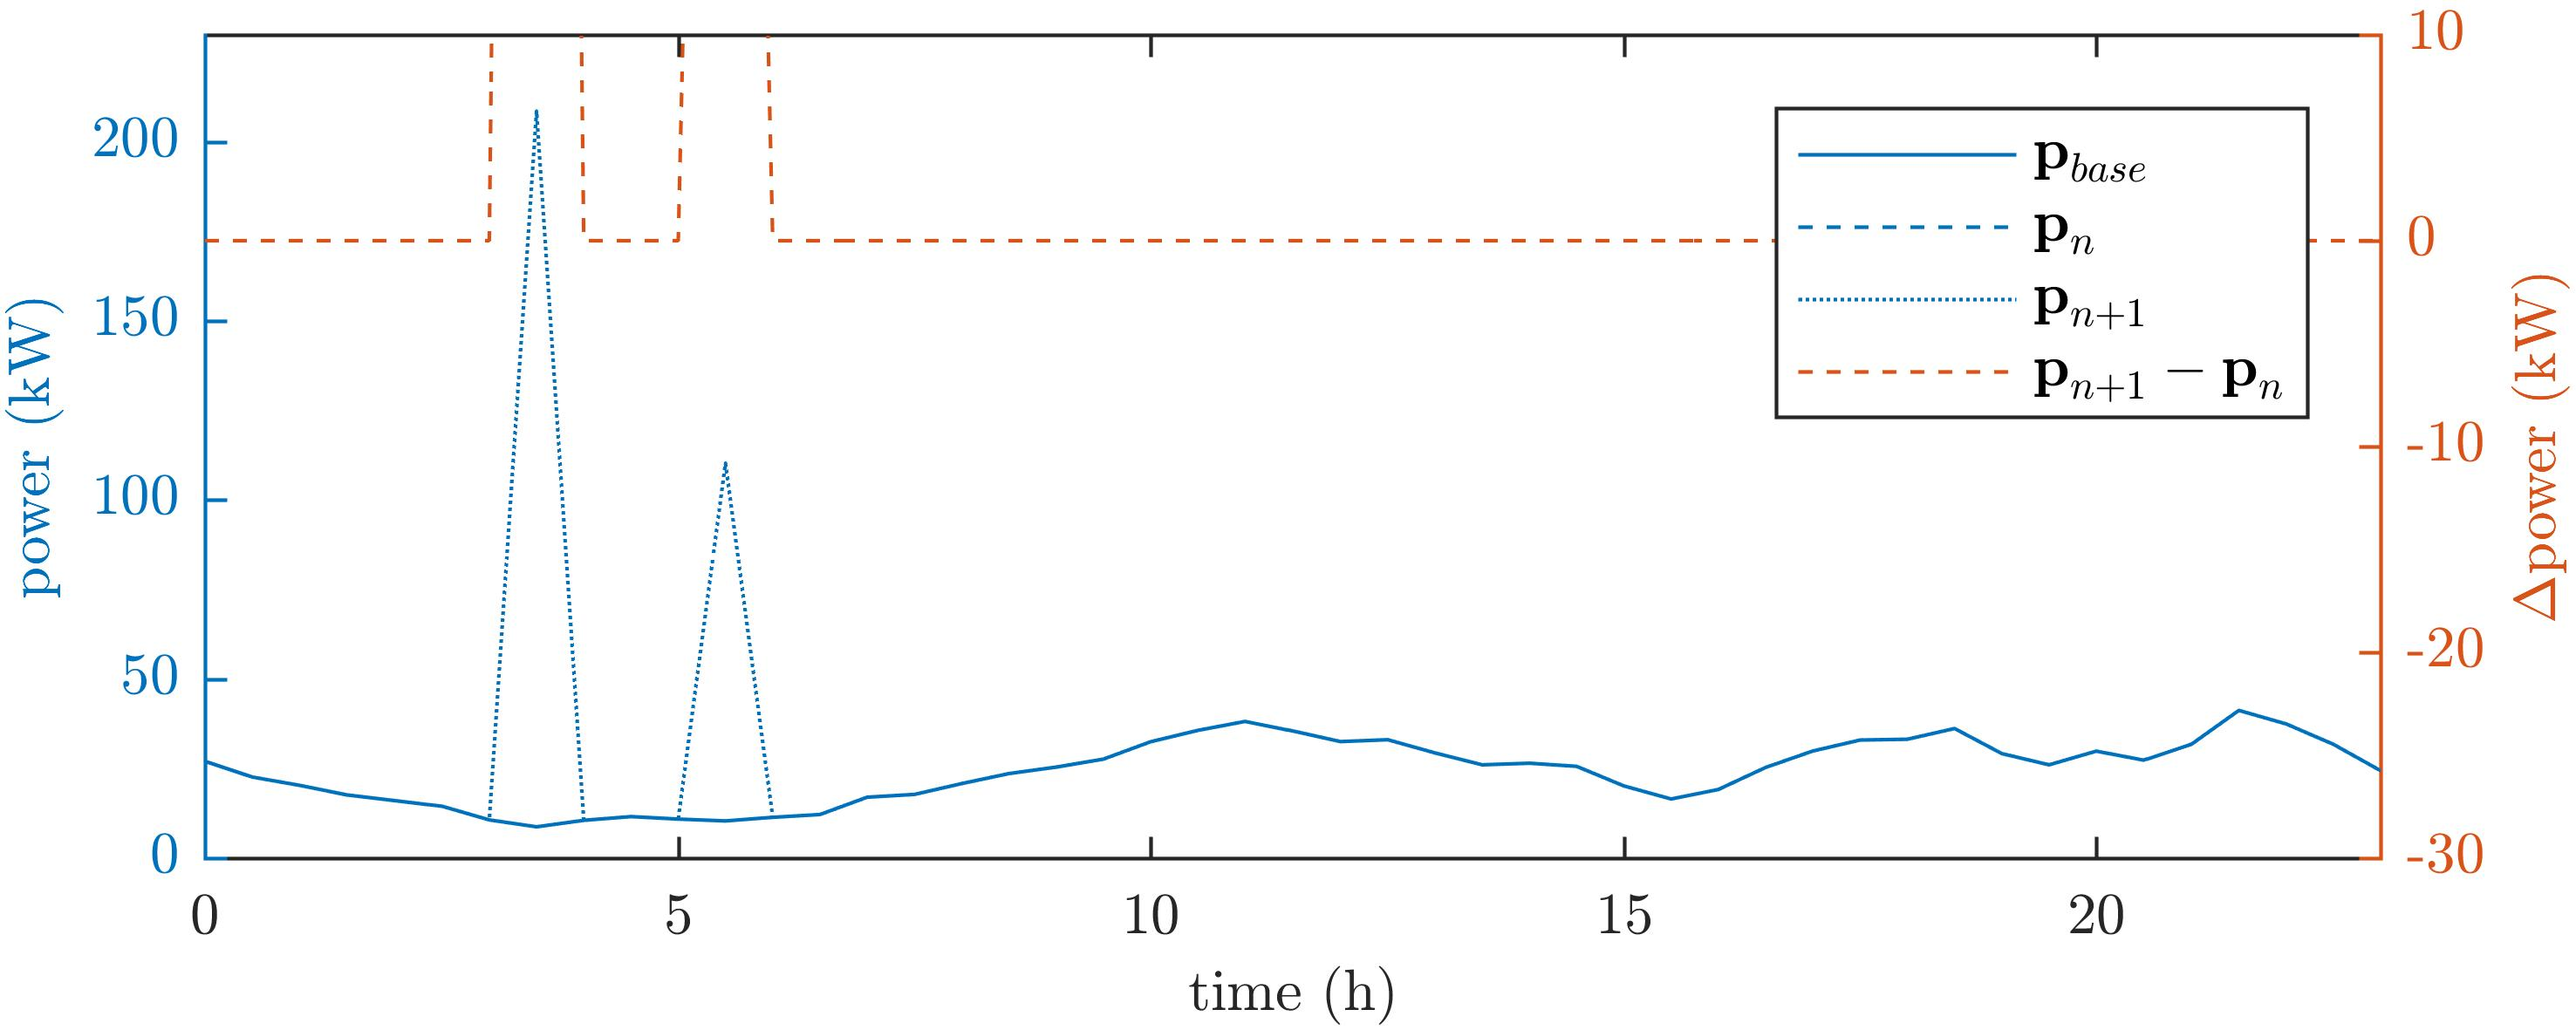
\includegraphics[height=4.5cm]{_chapter3/fig/time-series/ts-i0001}
		\label{ch3:subfig:time-series-1}
	}\\
	\subfloat[]{
		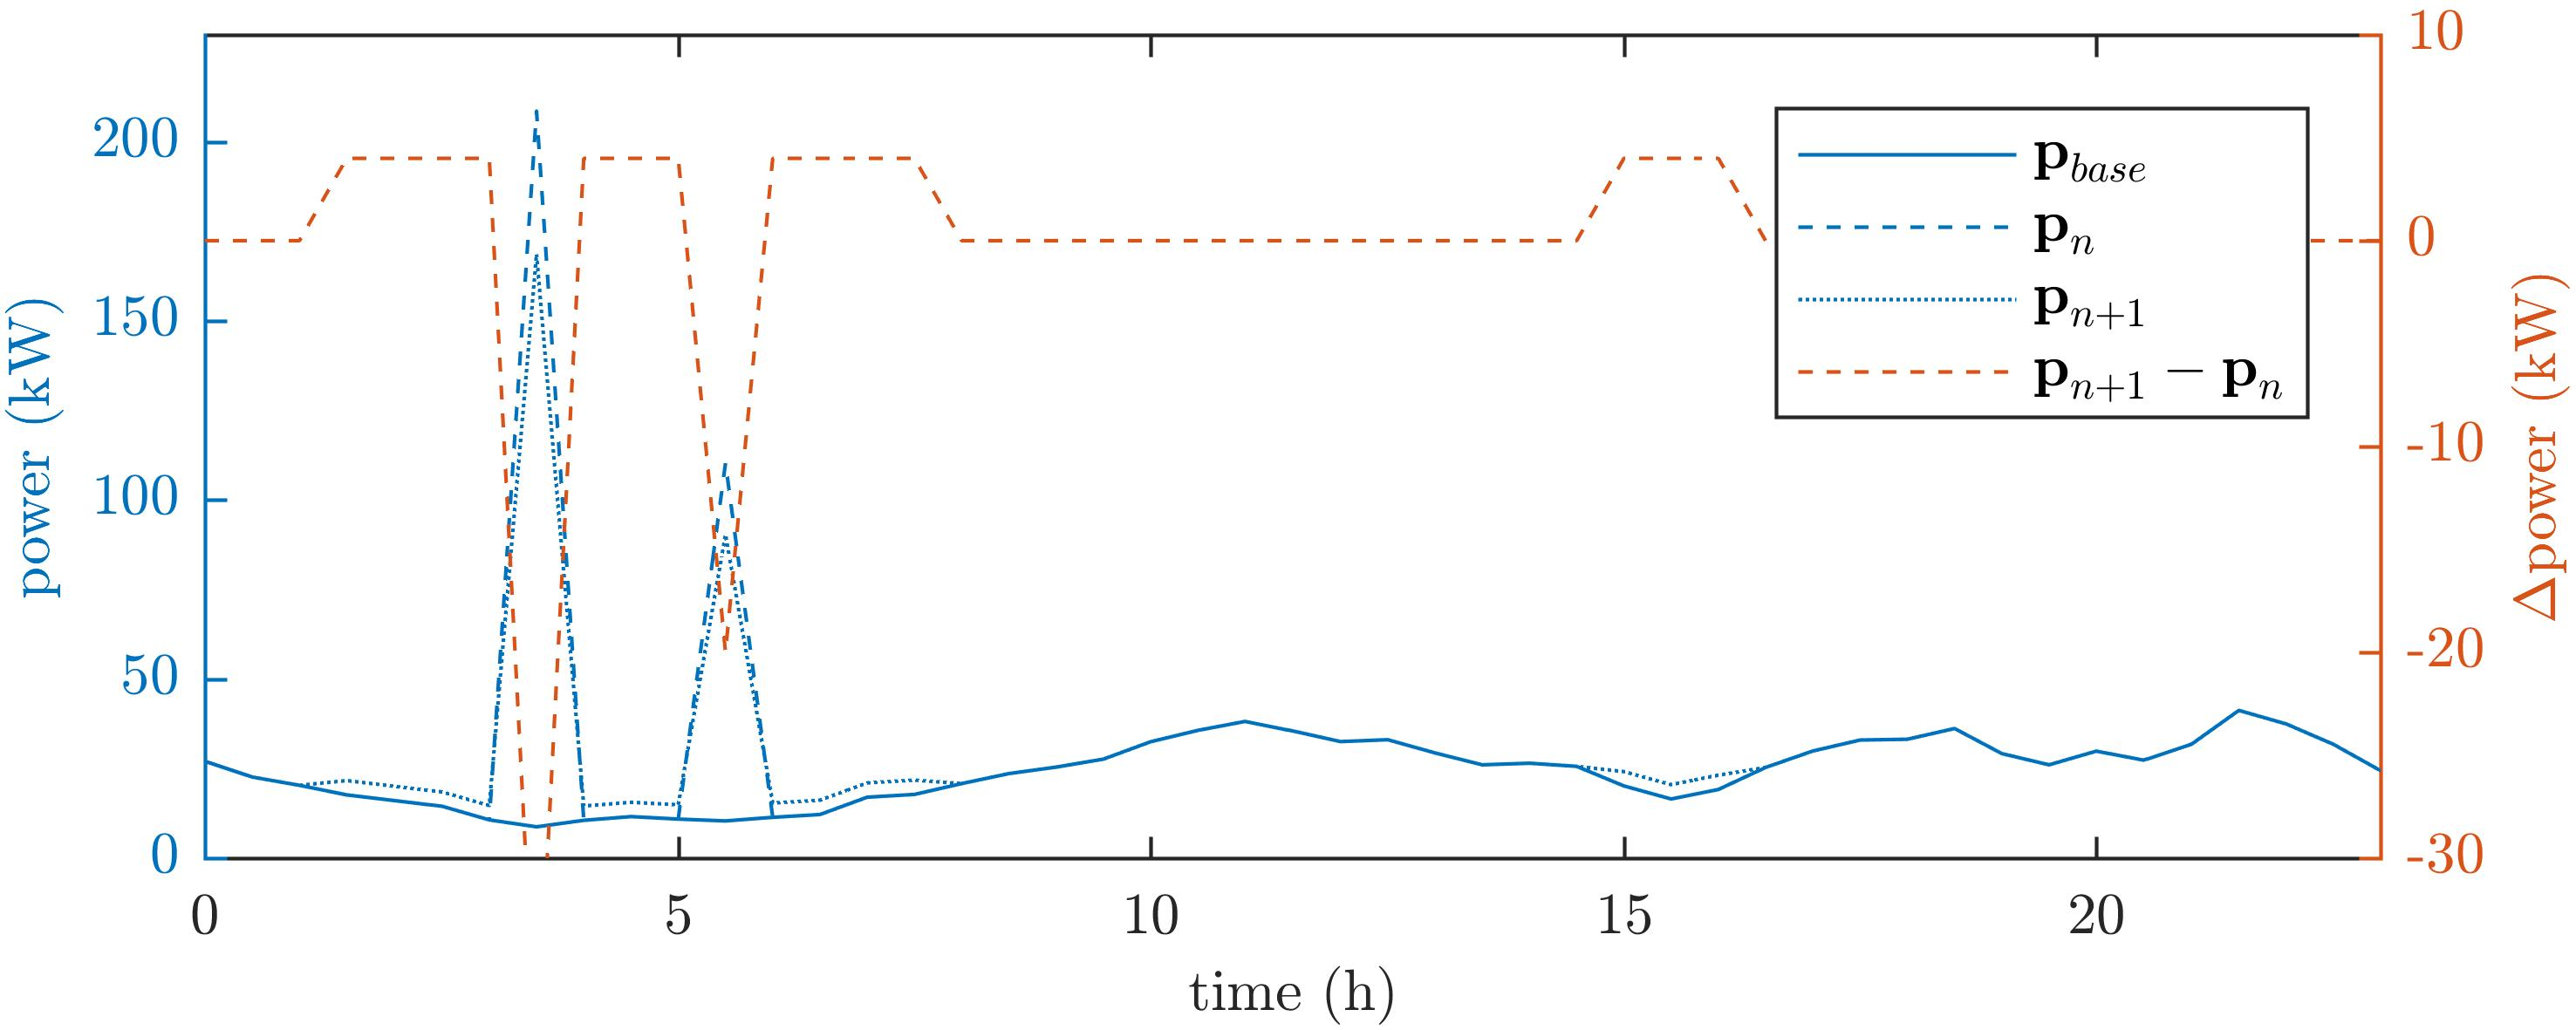
\includegraphics[height=4.5cm]{_chapter3/fig/time-series/ts-i0002}
		\label{ch3:subfig:time-series-2}
	}\\
	\subfloat[]{
		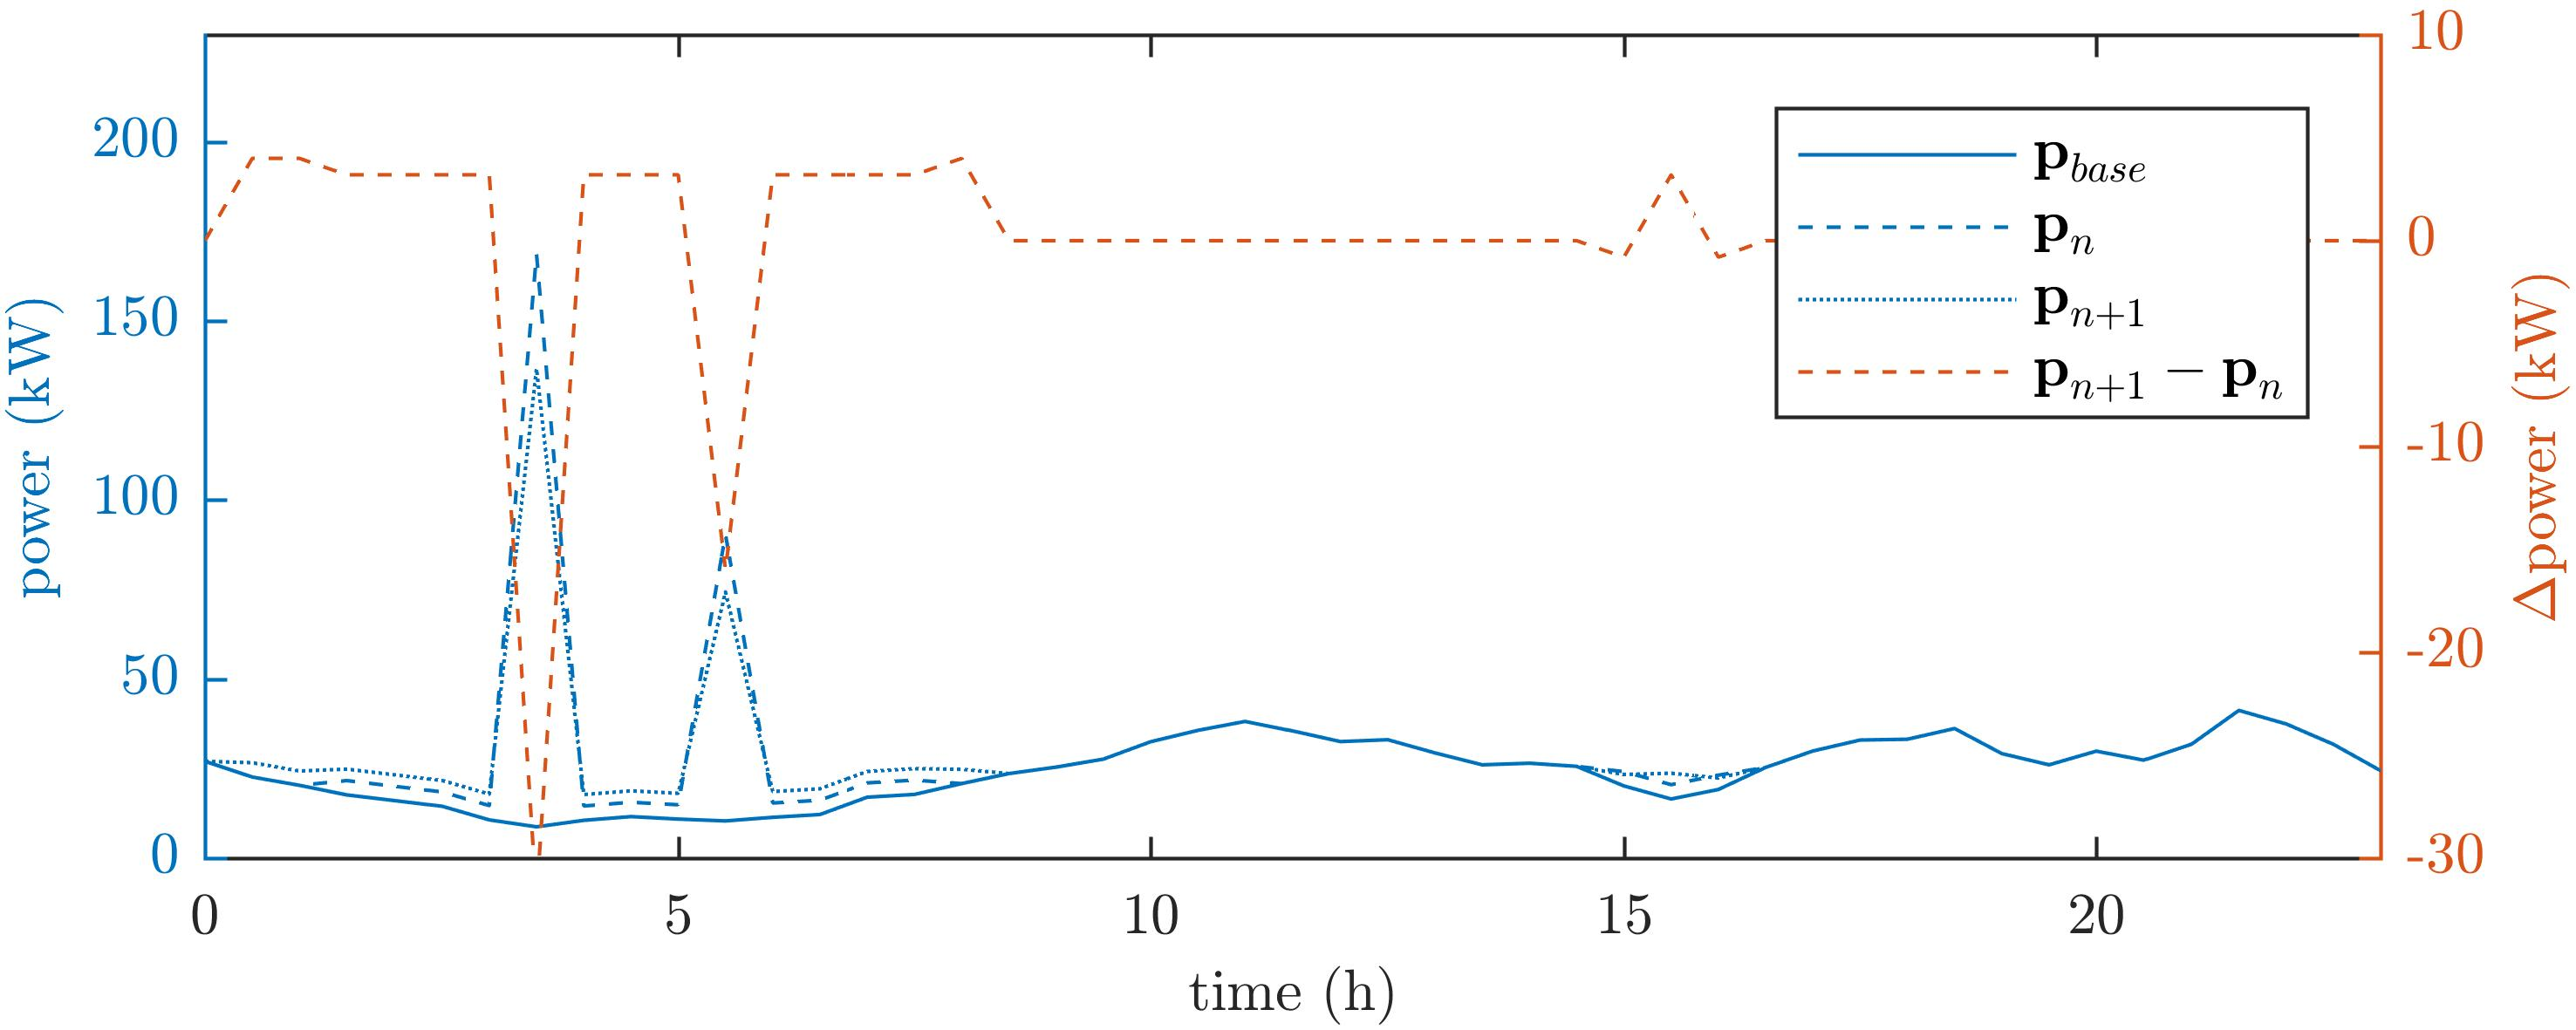
\includegraphics[height=4.5cm]{_chapter3/fig/time-series/ts-i0003}
		\label{ch3:subfig:time-series-3}
	}\\
	\subfloat[]{
		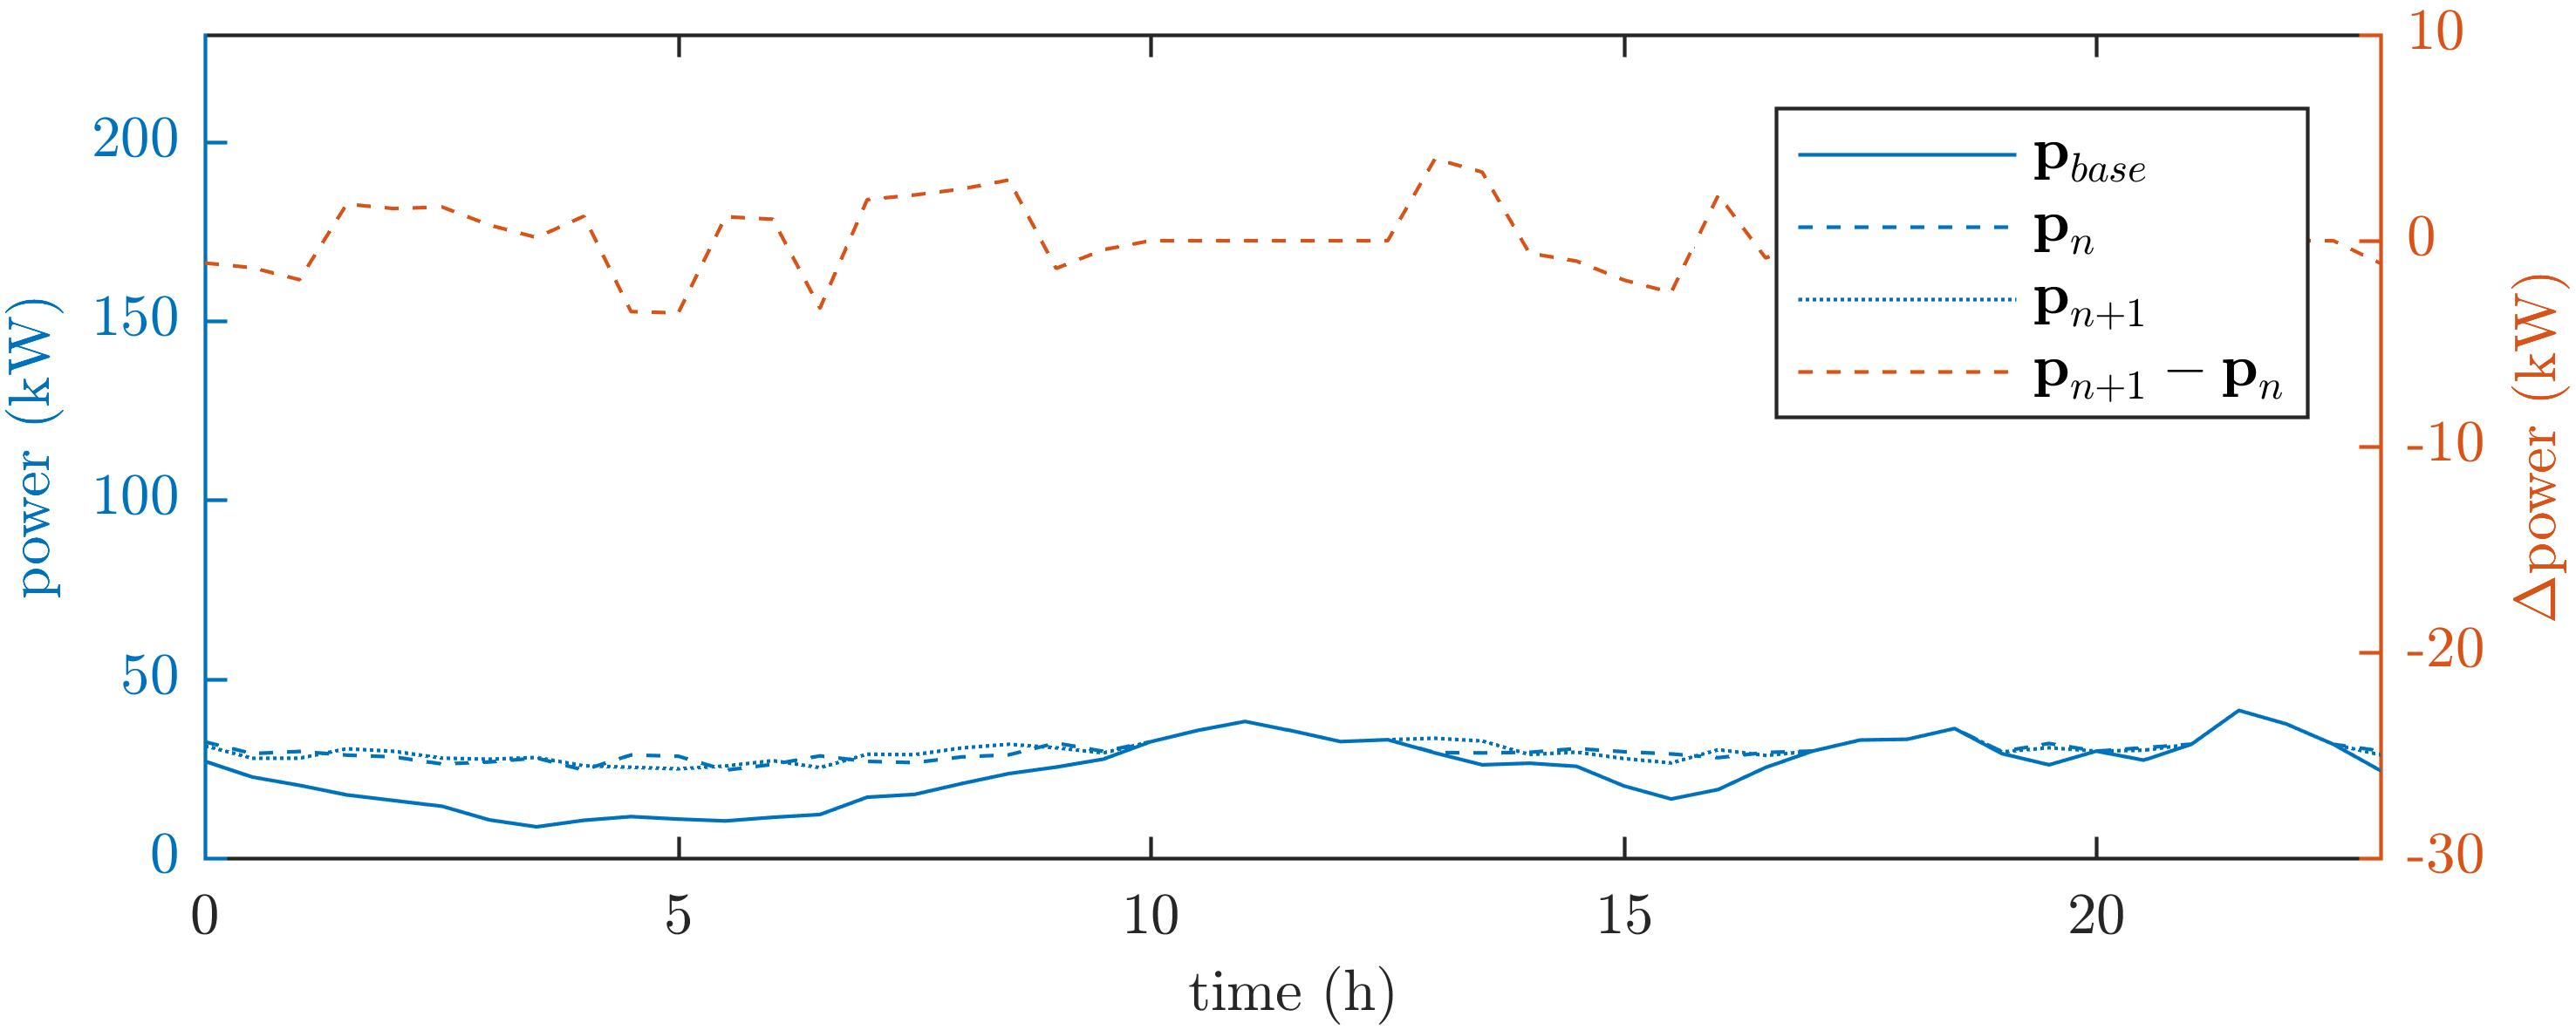
\includegraphics[height=4.5cm]{_chapter3/fig/time-series/ts-i0100}
		\label{ch3:subfig:time-series-last}
	}
\caption{Time series evolution for $\alpha=0.02$ and $\beta=0.20$, where (a) is at $n=1$, (b) is at $n=2$, (c) is at $n=3$, and (d) is at $n=N-1$.}
\label{ch3:fig:time-series}
\end{figure}

Here, the first algorithm iteration is shown in Figure~\ref{ch3:subfig:time-series-1}, where allocated power profile produces two new morning spikes of around 200kW and subsequently 110kW.
The second iteration however reduces these spikes by the factor $\alpha$ (i.e $0.2$) and redistributes the undone charging powers over the new power profile.
Figure~\ref{ch3:subfig:time-series-2} shows this reduction and reallocation.
Figure~\ref{ch3:subfig:time-series-3} is the third iteration that reduces and redistributes the peaks even further.
In the end (i.e. when $n=100$) the resulting power profile becomes as flat as possible which is shown in Figure~\ref{ch3:subfig:time-series-last}.
Throughout these iterations, it can be observed how the peak load in the total power (i.e. $\textbf{p}_n$) reduces and it can be observed how the changes in charging power (i.e. $\textbf{p}_{n+1}-\textbf{p}_n$) reduce in variance, which indicates that the algorithm works for the chosen parameters of $\alpha$ and $\beta$.
However, different parameters of $\alpha$ and $\beta$ do impact the performance of this synchronised algorithm execution as shown in Figure~\ref{ch3:fig:oscillation}.

\begin{figure}\centering
	\subfloat[]{
		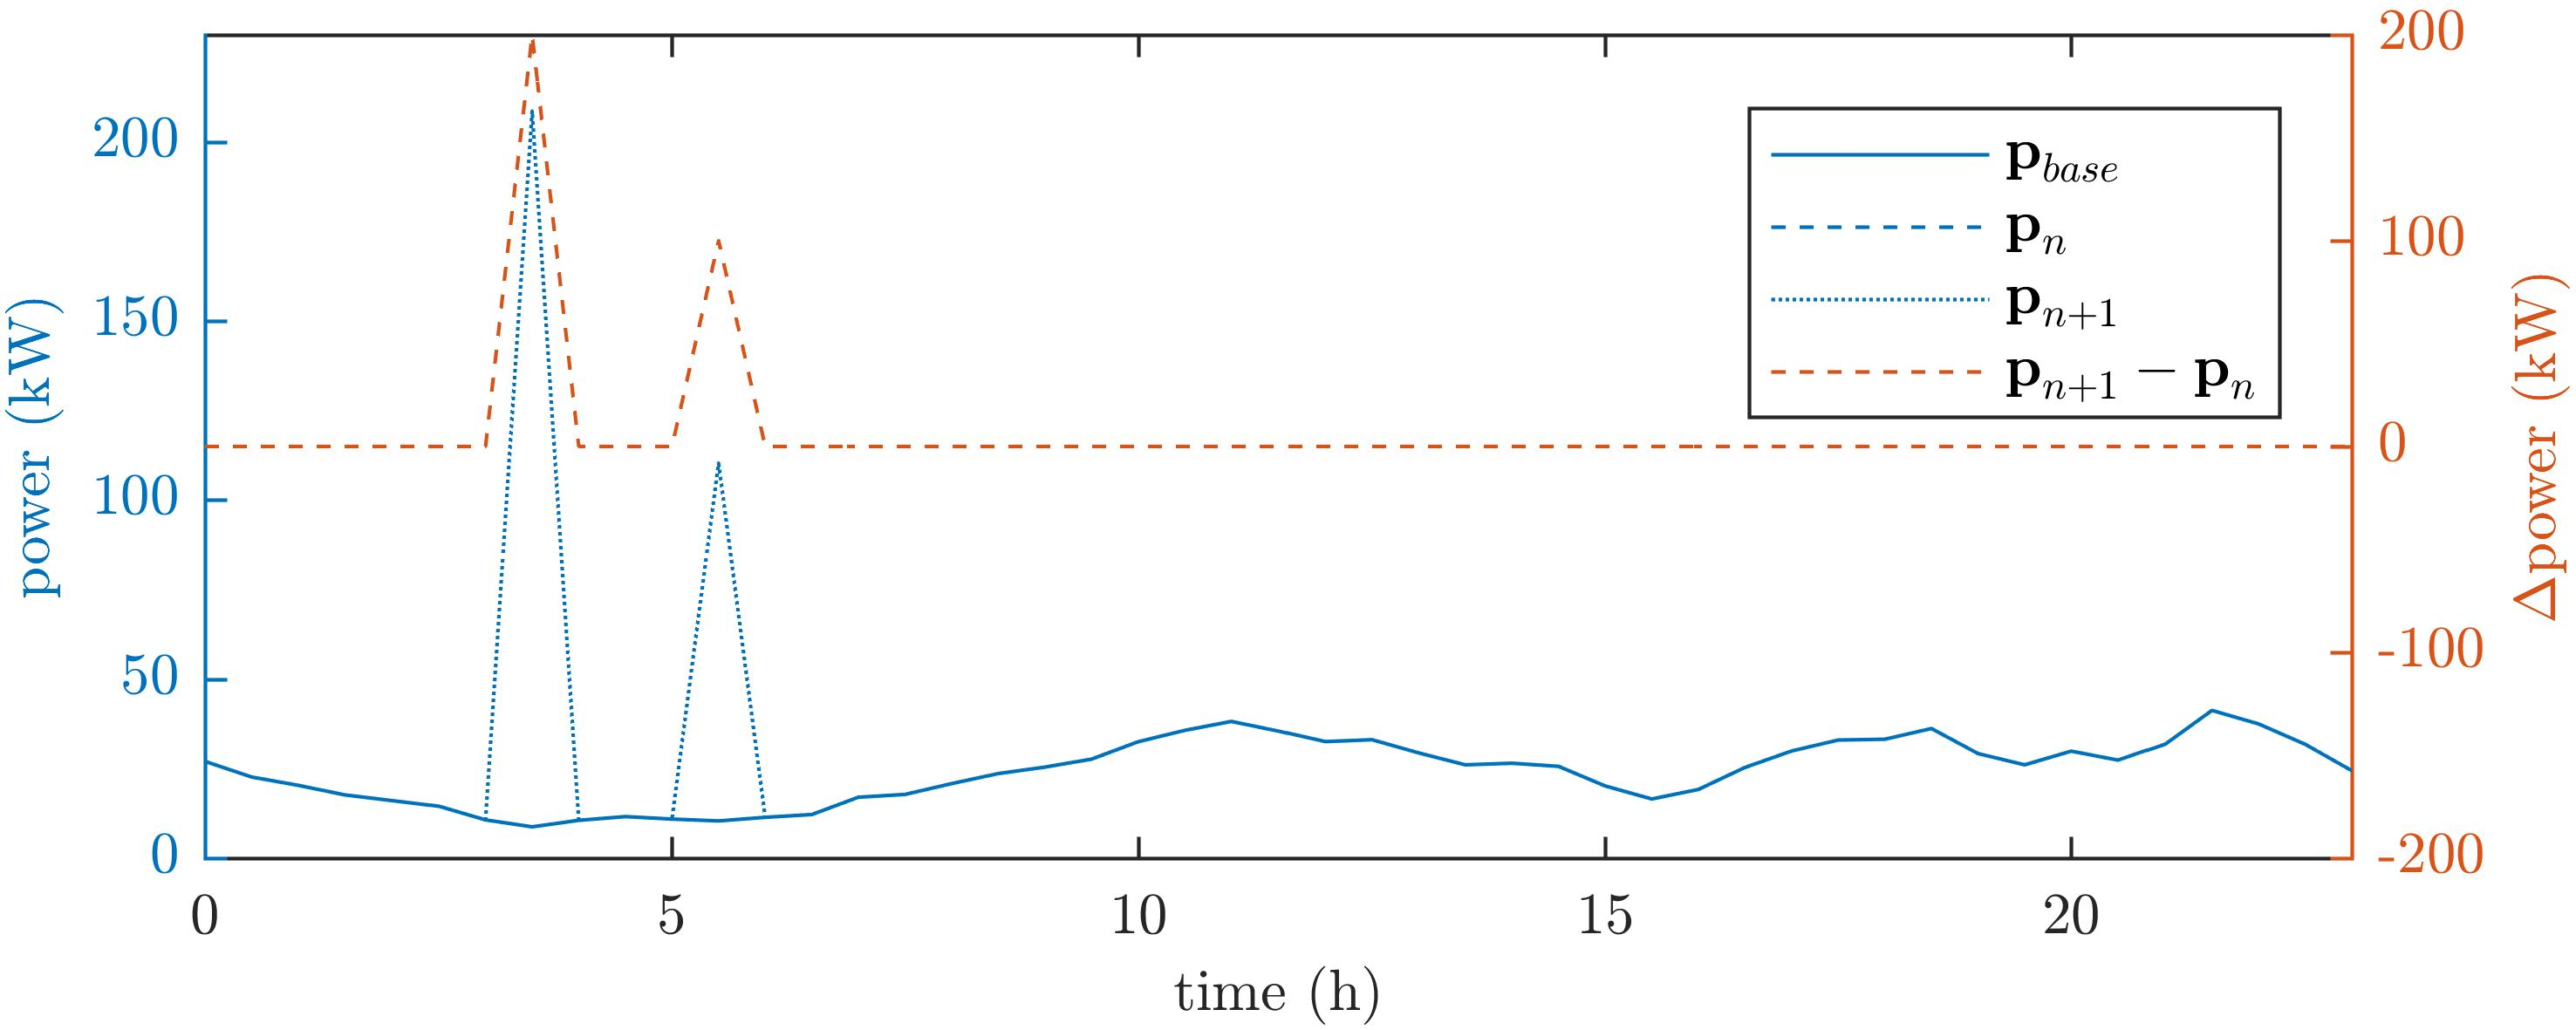
\includegraphics[height=4.5cm]{_chapter3/fig/oscillation/ts-i0001}
		\label{ch3:subfig:oscillation-1}
	}\\
	\subfloat[]{
		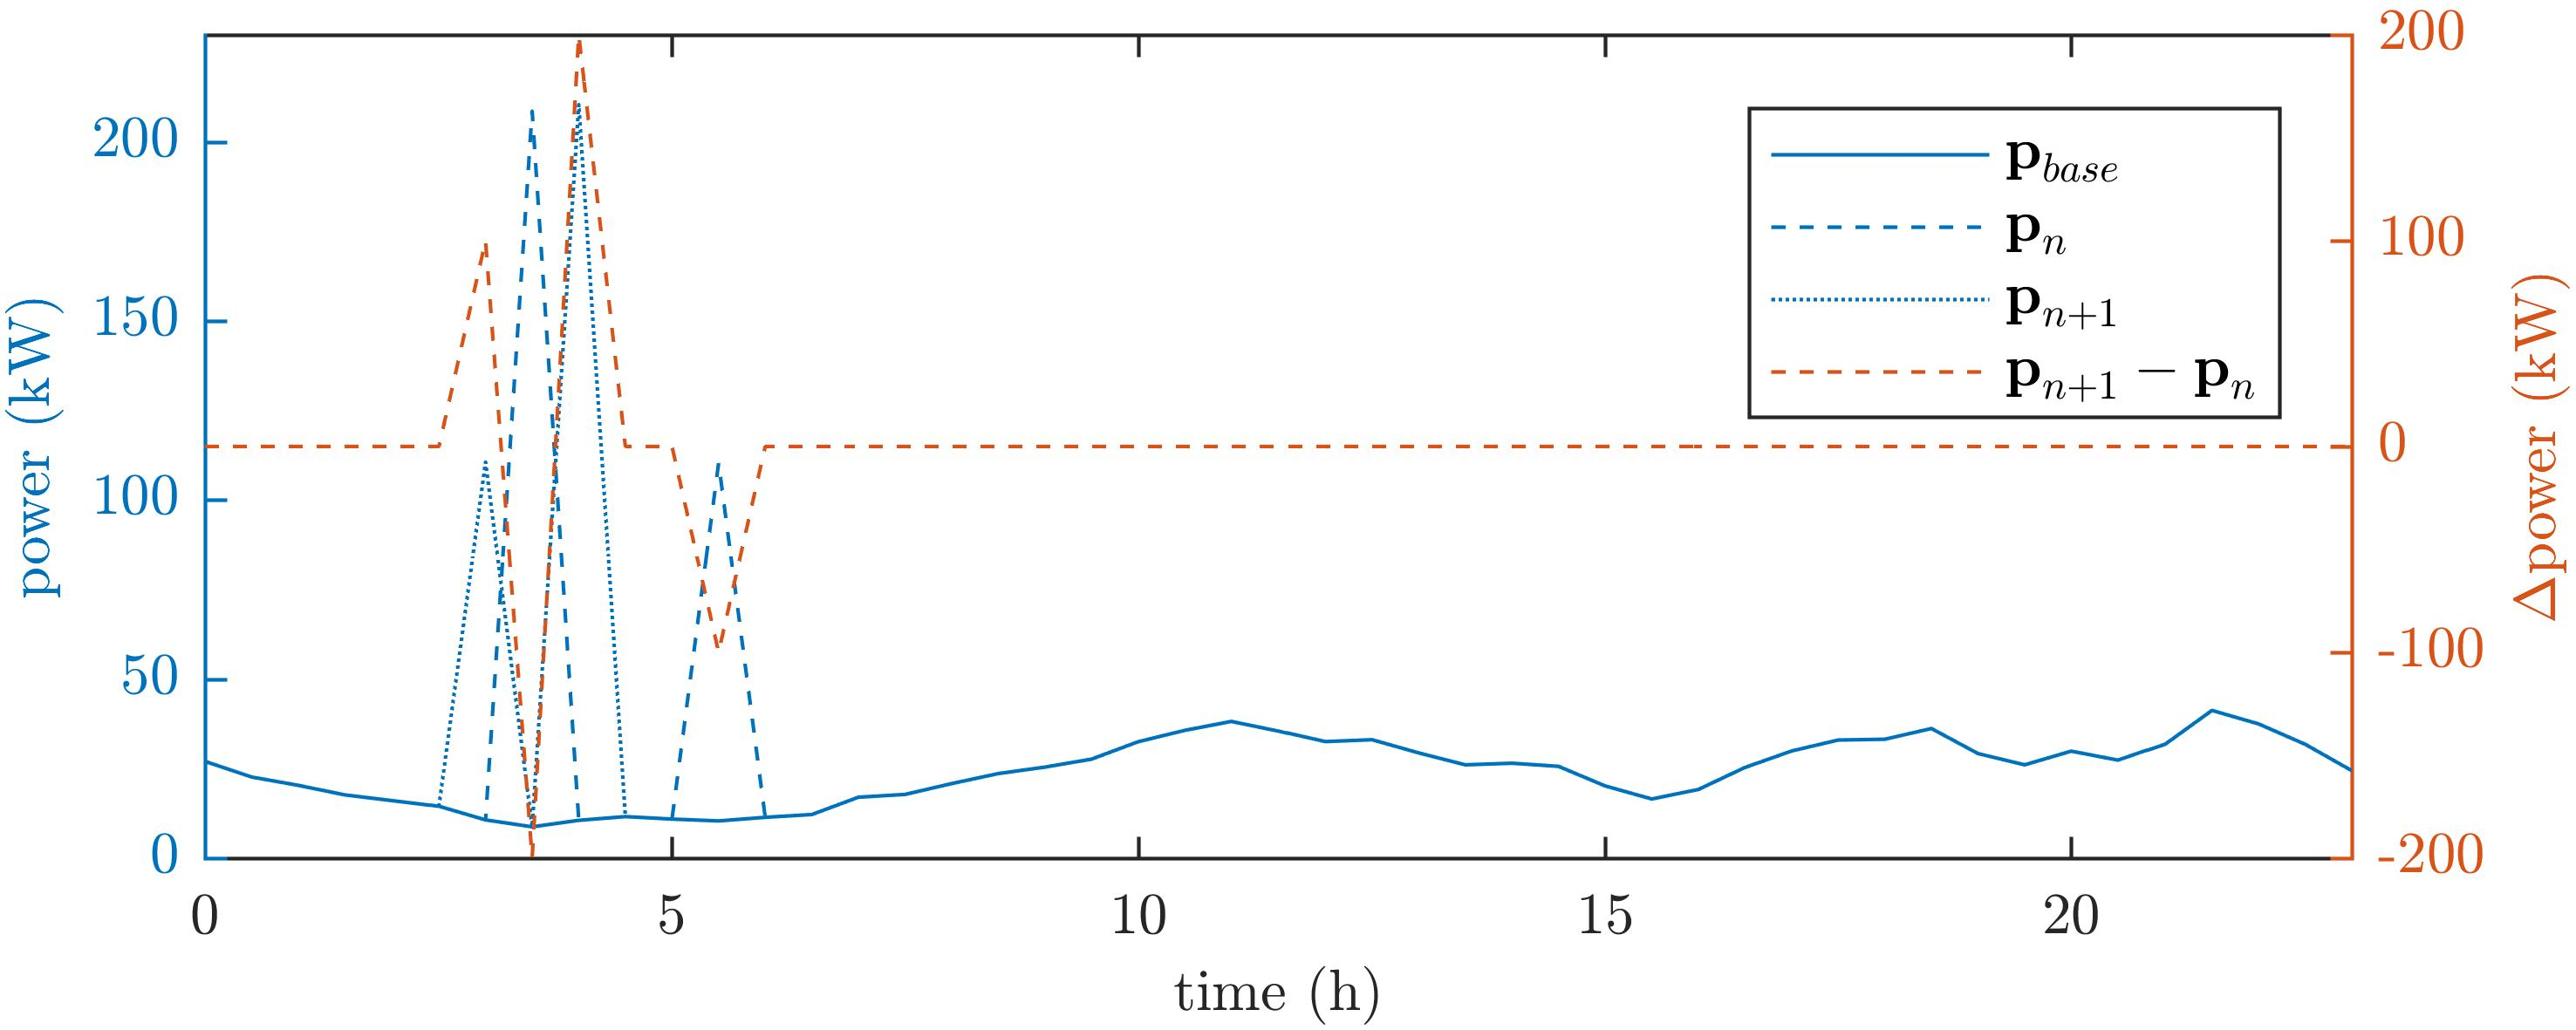
\includegraphics[height=4.5cm]{_chapter3/fig/oscillation/ts-i0002}
		\label{ch3:subfig:oscillation-2}
	}\\
	\subfloat[]{
		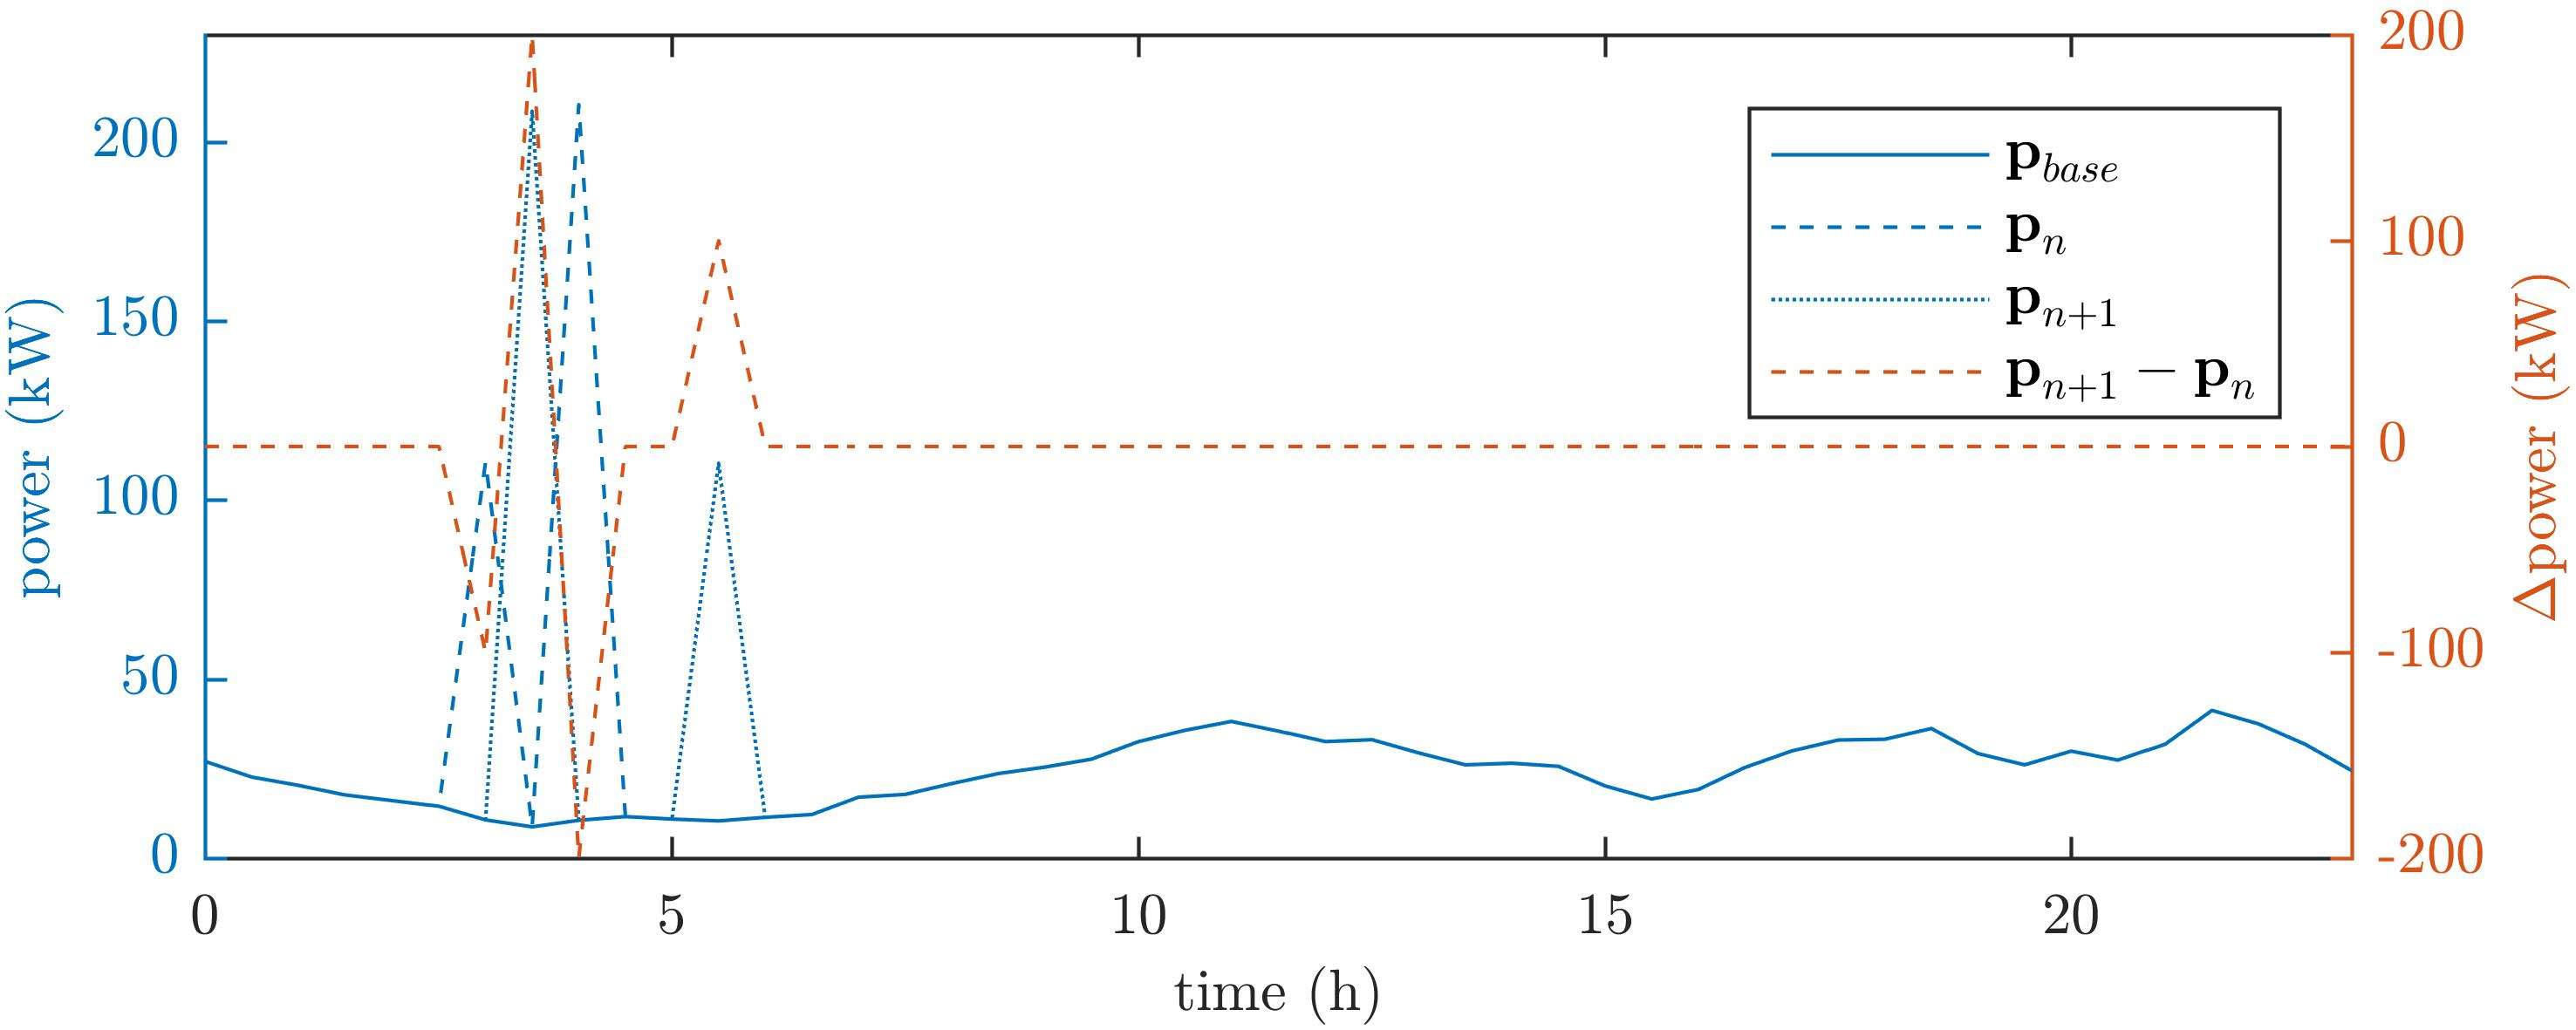
\includegraphics[height=4.5cm]{_chapter3/fig/oscillation/ts-i0003}
		\label{ch3:subfig:oscillation-3}
	}\\
	\subfloat[]{
		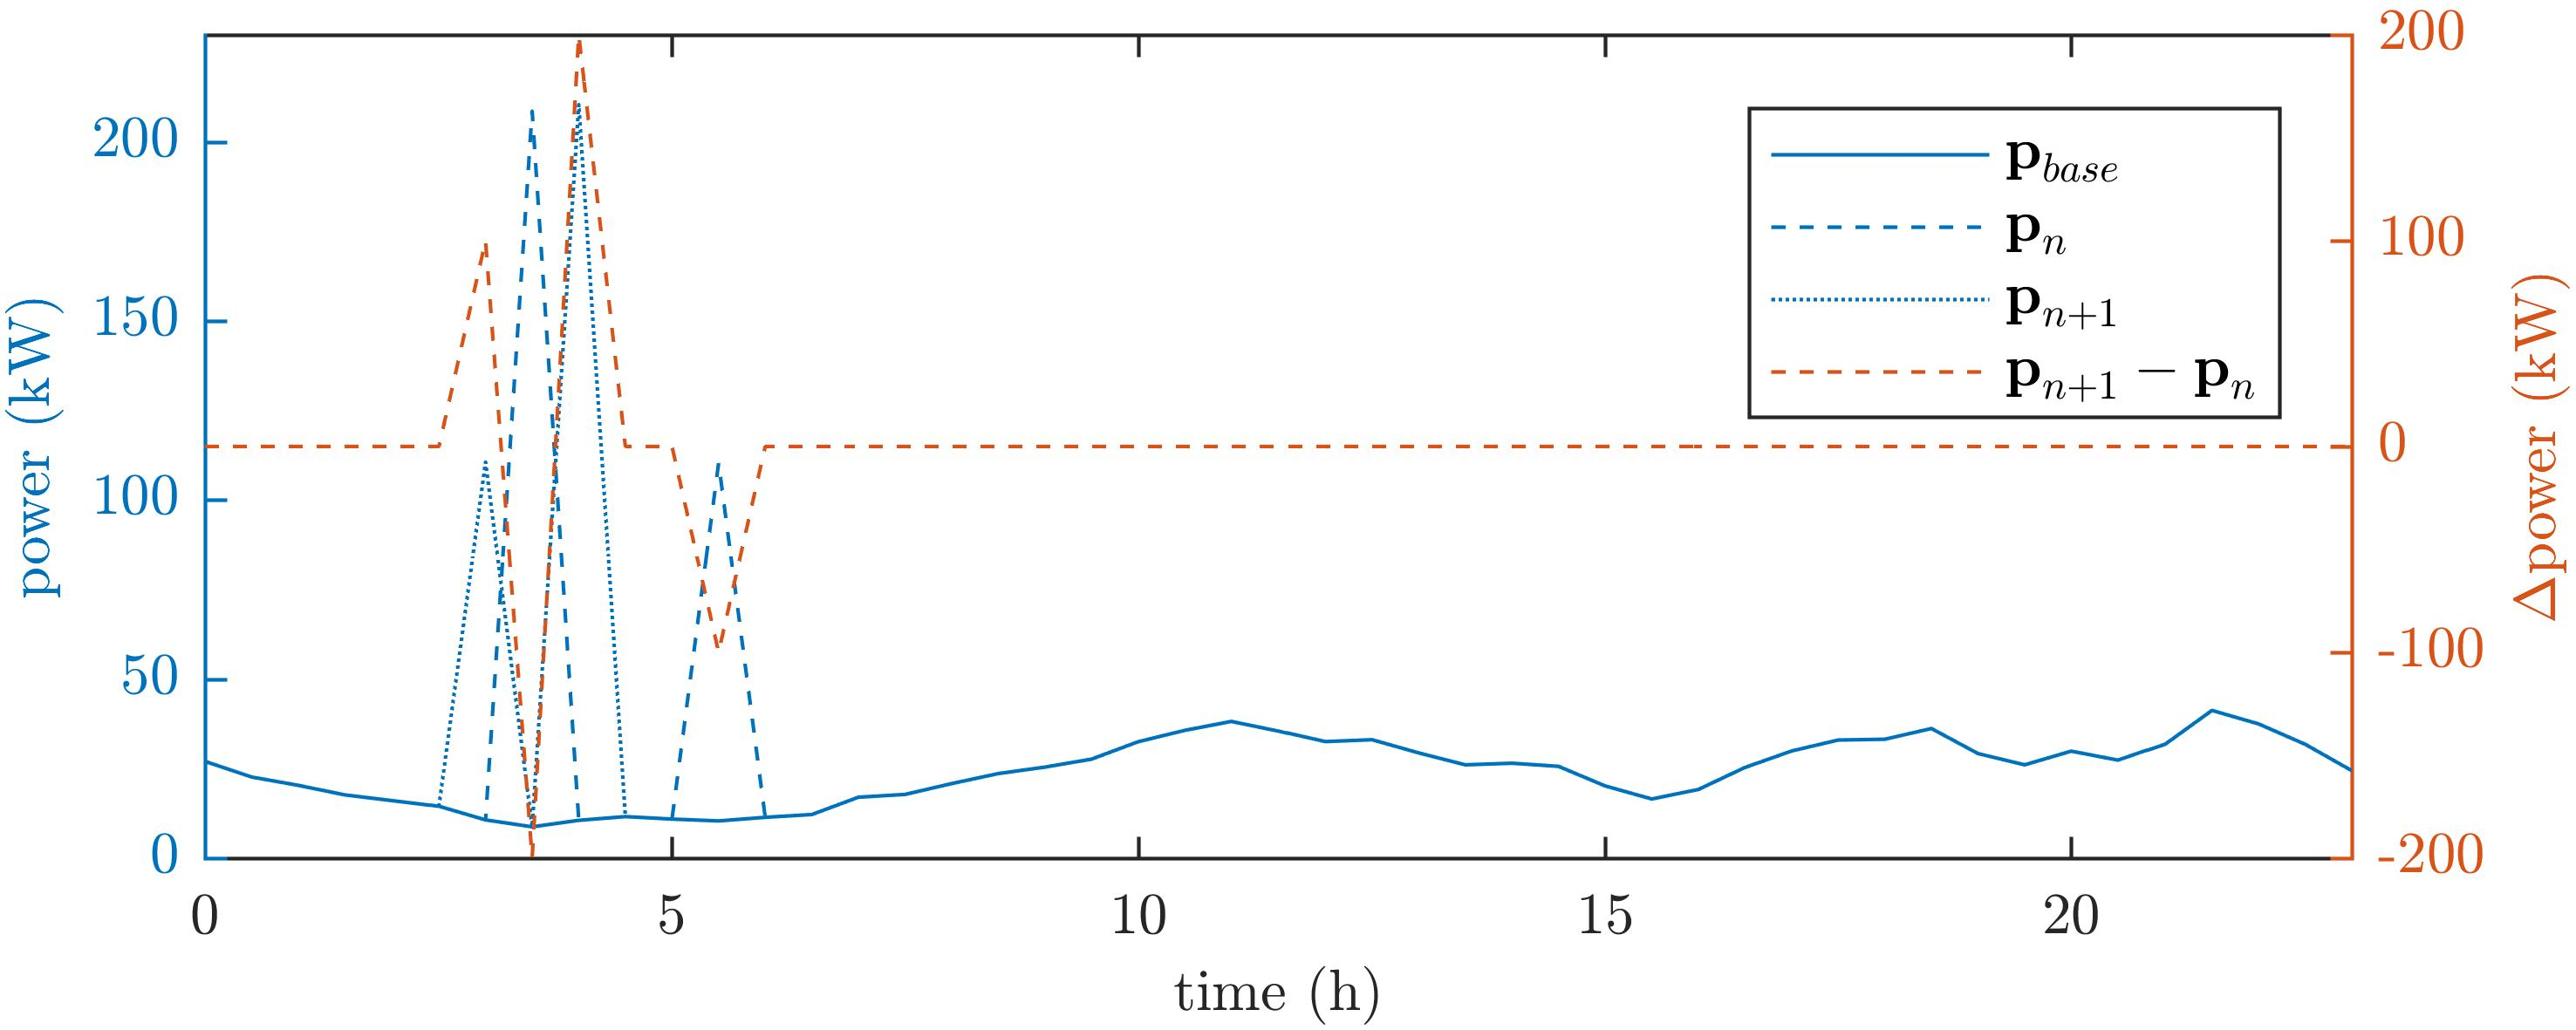
\includegraphics[height=4.5cm]{_chapter3/fig/oscillation/ts-i0100}
		\label{ch3:subfig:oscillation-last}
	}
\caption{Time series evolution for $\alpha=1.00$ and $\beta=1.00$, where (a) is at $n=1$, (b) is at $n=2$, (c) is at $n=3$, and (d) is at $n=N-1$.}
\label{ch3:fig:oscillation}
\end{figure}

\begin{table}\centering
	\begin{tabular}{r | C{2cm} C{2cm} | C{2cm} C{2cm}}
		\multirow{2}{*}{iteration ($n$)} & \multicolumn{2}{c|}{$\alpha=0.02$ and $\beta=0.20$} & \multicolumn{2}{c}{$\alpha=1.00$ and $\beta=1.00$} \\
	   & $\zeta_\text{PAR}$ & $\zeta_\text{TRA}$ & $\zeta_\text{PAR}$ & $\zeta_\text{TRA}$\\
	  	\hline
          1 & 46.84 & 45.86 & 46.84 & 45.86\\
          2 & 30.61 & 35.54 & 47.66 & 46.26\\
          3 & 20.10 & 27.31 & 46.84 & 45.86\\
          4 & 13.28 & 20.75 & 47.66 & 46.26\\
          5 & 8.83  & 15.56 & 46.84 & 45.86\\
          6 & 5.93  & 11.41 & 47.66 & 46.26\\
          7 & 4.02  & 8.20  & 46.84 & 45.86\\
          8 & 2.76  & 5.83  & 47.66 & 46.26\\
          9 & 1.92  & 4.24  & 46.84 & 45.86\\
         10 & 1.83  & 3.22  & 47.66 & 46.26\\
   $\vdots$ & $\vdots$ & $\vdots$ & $\vdots$ & $\vdots$\\
		100 & 1.83  & 2.72  & 47.66 & 46.26\\
   		\hline
   		\hline
   		convergence ($b$) & 0.47 & 0.32 & 0.00 & 0.00
	\end{tabular}
\sethlcolor{green}
	\caption{Comparison of $\zeta^\text{PAR}$ and $\zeta^\text{TRA}$ for two $\alpha$ and $\beta$ parameter pairs as shown in Figure~\ref{ch3:fig:oscillation} and Figure~\ref{ch3:fig:time-series}. Each value per iteration $n$ and the convergence $b$ is shown.}
	\label{ch3:tab:pair-comparison}
\end{table}

%  1 & 46.839871 & 45.855341 & 46.839871 & 45.855341\\
%  2 & 30.607134 & 35.537698 & 47.659842 & 46.257807\\
%  3 & 20.098148 & 27.310970 & 46.839871 & 45.855341\\
%  4 & 13.276370 & 20.747178 & 47.659842 & 46.257807\\
%  5 & 8.833609  & 15.564391 & 46.839871 & 45.855341\\
%  6 & 5.928785  & 11.409779 & 47.659842 & 46.257807\\
%  7 & 4.020532  & 8.204652  & 46.839871 & 45.855341\\
%  8 & 2.759917  & 5.831519  & 47.659842 & 46.257807\\
%  9 & 1.921657  & 4.239981  & 46.839871 & 45.855341\\
% 10 & 1.829655  & 3.223272  & 47.659842 & 46.257807\\
%100 & 1.829655  & 2.722986  & 47.659842 & 46.257807


Whereas the $\alpha$ and $\beta$ parameters use to produce the results in Figure~\ref{ch3:fig:time-series} reduced the power spike, those parameters in \ref{ch3:fig:oscillation} where $\alpha = \beta = 1.0$ did not.
In fact, an oscillating behaviour can be observed since the initially applied power profile is completely undone and completely reassigned onto a different demand trough.
Since this produces similar peaks, the same procedure repeats and reassigns the complete power profile back to the original demand troughs.
In the end, these charging spikes can never be fully mitigated and the algorithm did not smoothen the total demand.
The resulting charging spike of more than 200kW could therefore cause significant issues if \hlrem{e.g. }the underlying physical network has not been scaled appropriately\hladd{, for example}.
This longevity of issue becomes more evident when comparing the $\zeta^\text{PAR}$ and $\zeta^\text{TRA}$ values for both parameter pairs.
The evolution of $\zeta^\text{PAR}$ and $\zeta^\text{TRA}$, as tabulated in Table~\ref{ch3:tab:pair-comparison}, shows this difference in performance and convergence of the algorithm when subjected to different values of $\alpha$ and $\beta$.
Those figures indicate that a well chosen pair of $\alpha$ and $\beta$ results in a convergence value (i.e. $b$) that is greater than zero.
No convergence occurred however for those values of $\alpha$ and $\beta$ that resulted in the oscillating behaviour (i.e. convergence rate $b$ is zero).

Next, the entire range of $\alpha$ and $\beta$ needed to be studied since different parameter pairs are likely to result in different convergence rates (and therefore different algorithm performance).
These results (i.e. for the synchronised algorithm performance) are plotted in Figure~\ref{ch3:fig:all-sync}.

\begin{figure}\centering
	\subfloat[]{
		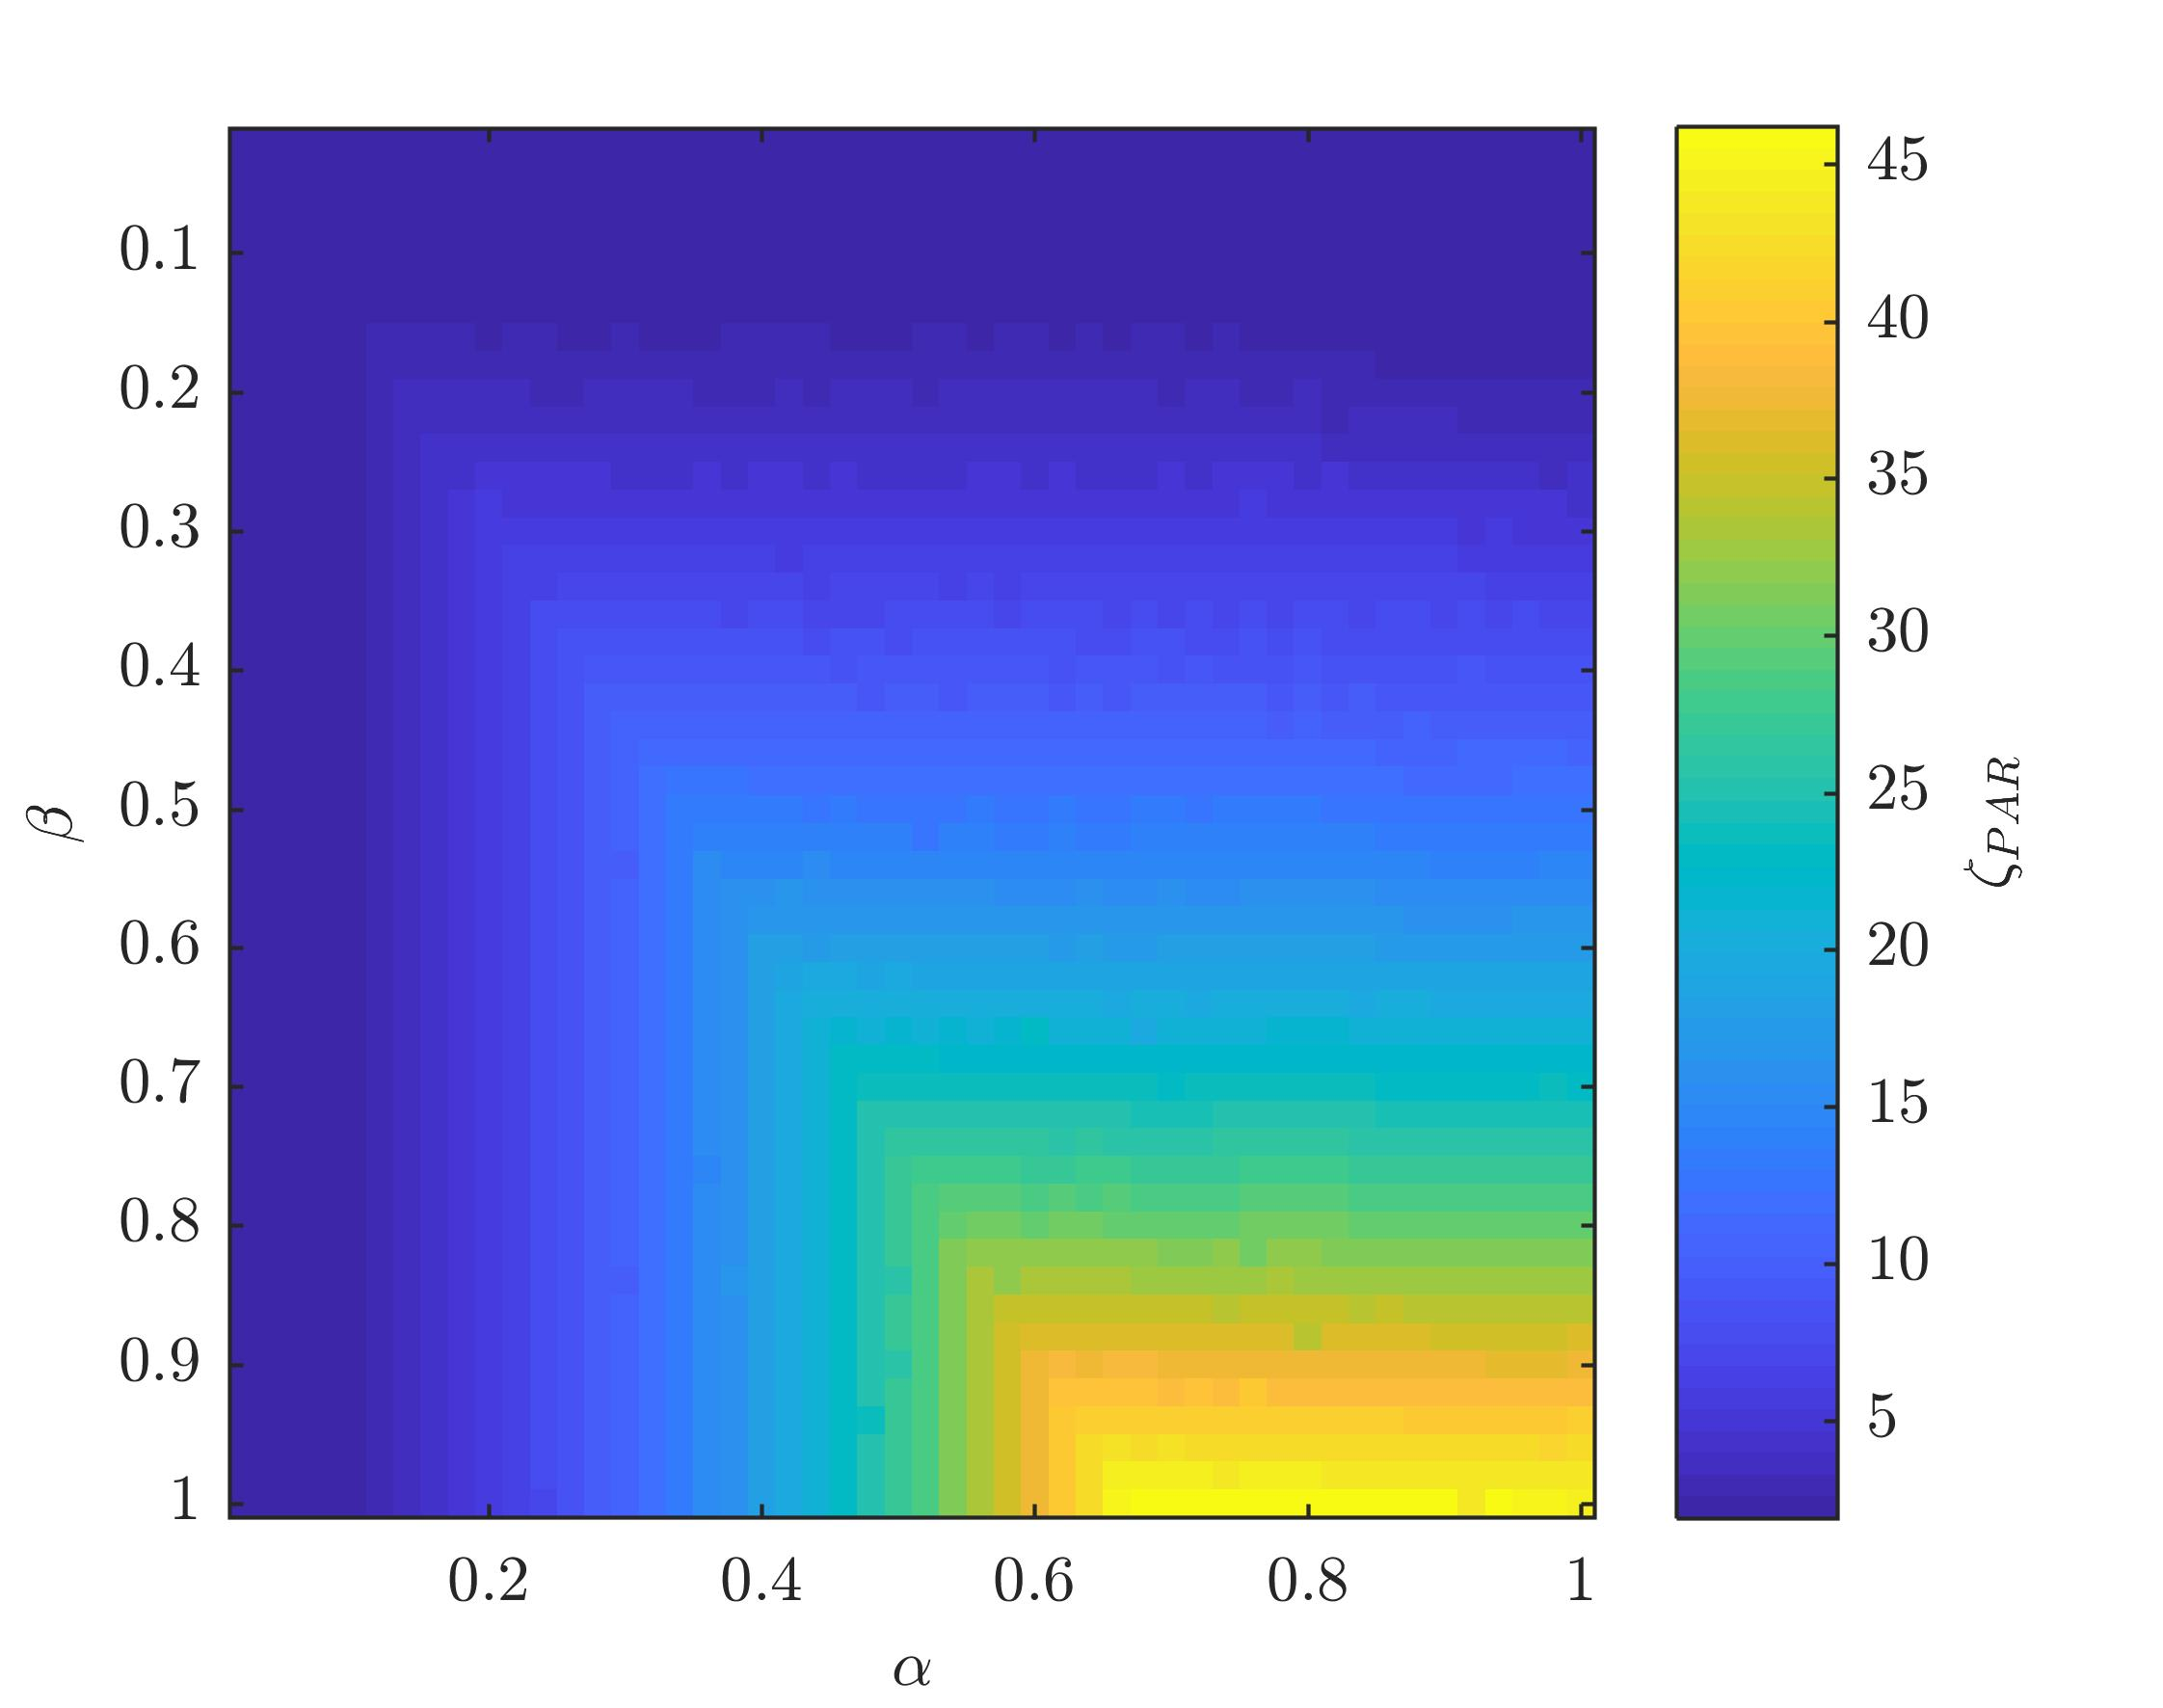
\includegraphics[width=0.5\linewidth]{_chapter3/fig/all-sync/3-all_par}
		\label{ch3:subfig:all-sync-par}
	}
	\subfloat[]{
		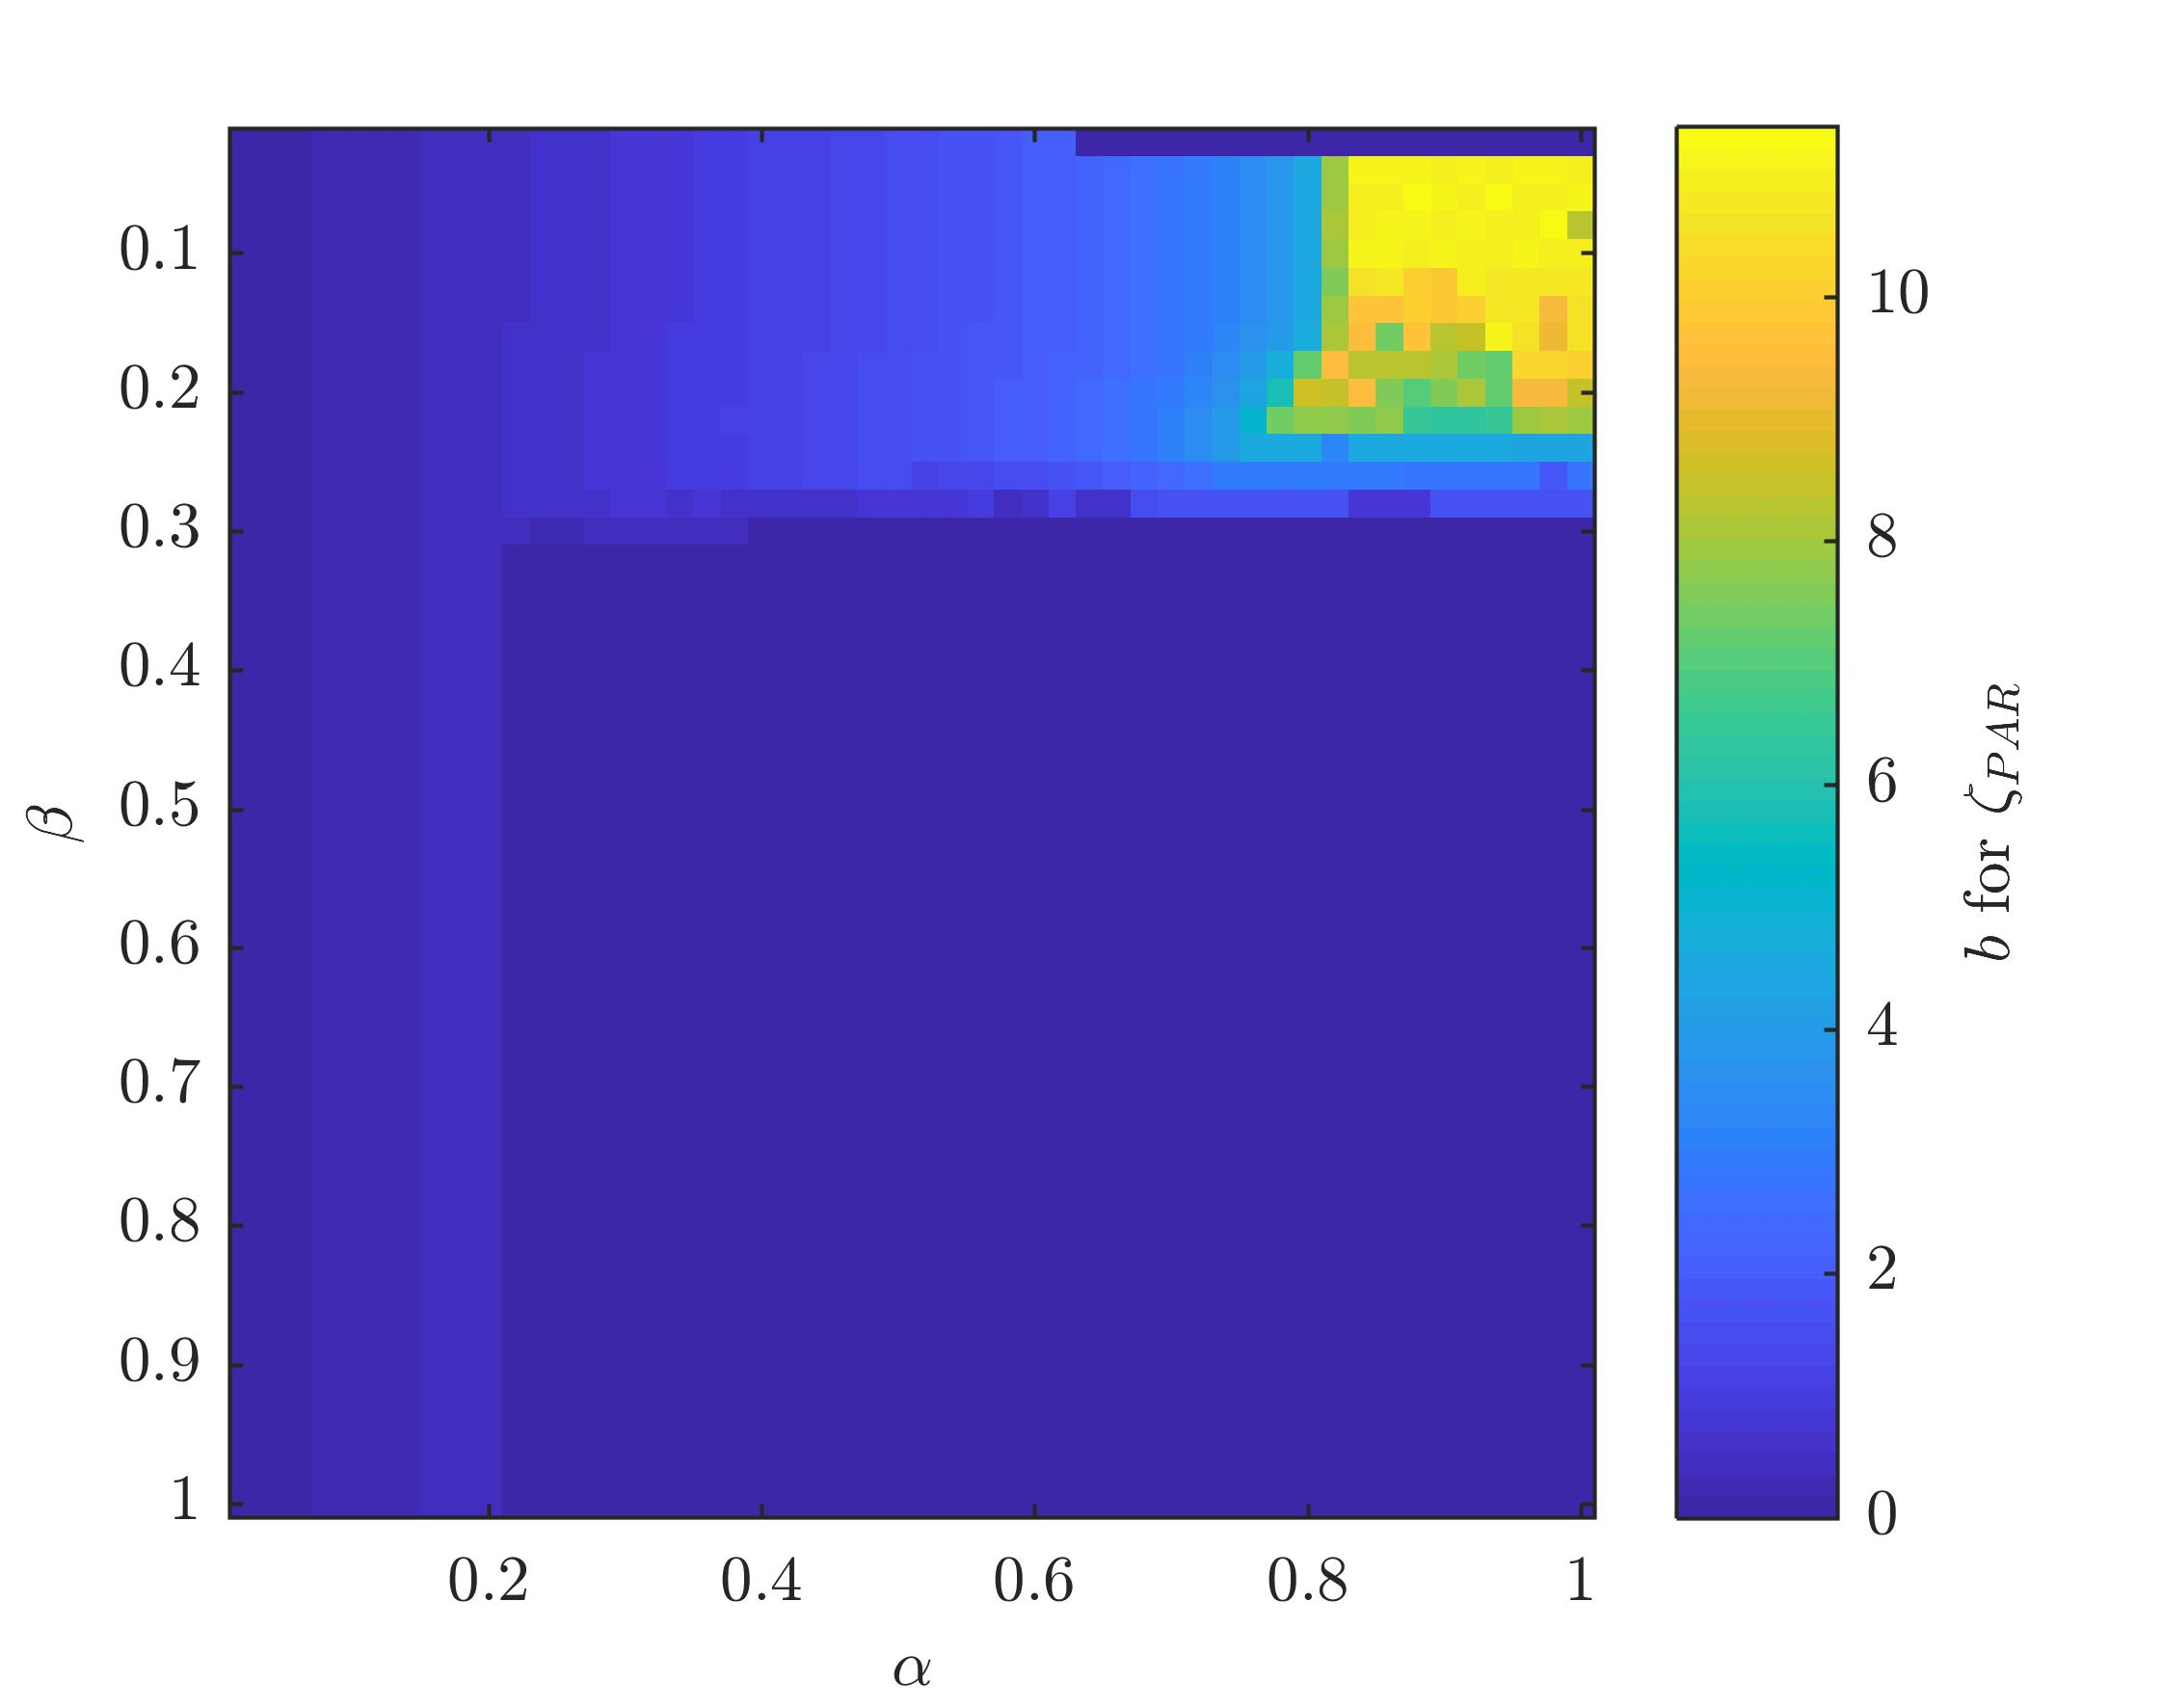
\includegraphics[width=0.5\linewidth]{_chapter3/fig/all-sync/3-all_par_conv}
		\label{ch3:subfig:all-sync-par-conv}
	}\\
	\subfloat[]{
		\includegraphics[width=0.5\linewidth]{_chapter3/fig/all-sync/3-all_tra}
		\label{ch3:subfig:all-sync-tra}
	}
	\subfloat[]{
		\includegraphics[width=0.5\linewidth]{_chapter3/fig/all-sync/3-all_tra_conv}
		\label{ch3:subfig:all-sync-tra-conv}
	}\\
	\caption{Full range analysis of $\alpha$ and $\beta$ where, (a) shows the final $\zeta_\text{PAR}$, (b) shows the convergence, $b$, for $\zeta_\text{PAR}$, (c) shows the final $\zeta_\text{TRA}$, and (d) shows the convergence, $b$, for $\zeta_\text{TRA}$ (red indicates missing data).}
	\label{ch3:fig:all-sync}
\end{figure}

Figure~\ref{ch3:subfig:all-sync-par} and Figure~\ref{ch3:subfig:all-sync-tra} show how the final values for both $\zeta^\text{PAR}$ and $\zeta^\text{TRA}$ were lowest when either $\alpha$ or $\beta$ was chosen closer to zero.
This result coincides with the finding that hard reduction and reallocation lead to an oscillating behaviour of the algorithm.
Similarly, the convergence of those two performance metrics, as shown in Figure~\ref{ch3:subfig:all-sync-par-conv} and Figure~\ref{ch3:subfig:all-sync-tra-conv}, was highest when $\alpha$ approached one and $\beta$ approached zero.
This behaviour is by design since a larger value of $\alpha$ increases the rate at which the currently applied peak is reduced whilst a smaller value of $\beta$ limits the amount that can be reallocated for each time slot.
Such clear behavioural differences for different pairs of $\alpha$ and $\beta$ indicate an optimal operation region of the algorithm within the north-eastern quadrant of the plot.
Whether the algorithm still performs in this way when introducing desynchronisation is answered in the subsequent section, Section~\ref{ch3:subsec:algorithm-performance-desynchronised-regular}.


\subsection{Algorithm performance for desynchronised operation with regular timing}
\label{ch3:subsec:algorithm-performance-desynchronised-regular}

\begin{figure}\centering
	\subfloat[]{
		\includegraphics{_chapter3/fig/time-series-desync/as-r-ts-i0001}
		\label{ch3:subfig:time-series-desync-1}
	}\\
	\subfloat[]{
		\includegraphics{_chapter3/fig/time-series-desync/as-r-ts-i0002}
		\label{ch3:subfig:time-series-desync-2}
	}\\
	\subfloat[]{
		\includegraphics{_chapter3/fig/time-series-desync/as-r-ts-i0003}
		\label{ch3:subfig:time-series-desync-3}
	}\\
	\subfloat[]{
		\includegraphics{_chapter3/fig/time-series-desync/as-r-ts-i0100}
		\label{ch3:subfig:time-series-desync-last}
	}
	\caption{Desynchronised time series evolution for $\alpha=0.02$ and $\beta=0.20$, where (a) is at $n=1$, (b) is at $n=2$, (c) is at $n=3$, and (d) is at $n=N-1$.}
	\label{ch3:fig:time-series-desync}
\end{figure}

Looking at the evolution of the time-series when desynchronising the algorithm's execution shows significant differences already.
Figure~\ref{ch3:fig:time-series-desync} shows thie evolution for the same parameters as those chosen for Figure~\ref{ch3:fig:time-series}.
The difference is however that the assignment of charging powers lead to a significantly lower demand spike at the very beginning of executing the algorithm.
Subsequent iterations then reduce this spike much broader than it has been the case when executing the algorithm in a synchronised manner.
Therefore, more demand troughs are filled and a smoother profile is obtained much quicker when compared to the synchronised case.

\begin{figure}\centering
	\subfloat[]{
		\includegraphics[width=0.5\linewidth]{_chapter3/fig/all-async-regular/2-all_par}
		\label{ch3:subfig:all-async-regular-par}
	}
	\subfloat[]{
		\includegraphics[width=0.5\linewidth]{_chapter3/fig/all-async-regular/2-all_par_conv}
		\label{ch3:subfig:all-async-regular-par-conv}
	}\\
	\subfloat[]{
		\includegraphics[width=0.5\linewidth]{_chapter3/fig/all-async-regular/2-all_tra}
		\label{ch3:subfig:all-async-regular-tra}
	}
	\subfloat[]{
		\includegraphics[width=0.5\linewidth]{_chapter3/fig/all-async-regular/2-all_tra_conv}
		\label{ch3:subfig:all-async-regular-tra-conv}
	}\\
	\caption{Full range analysis of $\alpha$ and $\beta$ for the desynchronised MAS where, (a) shows the final $\zeta_\text{PAR}$, (b) shows the convergence, $b$, for $\zeta_\text{PAR}$, (c) shows the final $\zeta_\text{TRA}$, and (d) shows the convergence, $b$, for $\zeta_\text{TRA}$ (red indicates missing data).}
	\label{ch3:fig:all-async-regular}
\end{figure}

This behaviour becomes particularly apparent when looking at the full range of $\alpha$ and $\beta$ values.
Figure~\ref{ch3:fig:all-async-regular} shows the same full range analysis as the figure in the previous section did, i.e. Figure~\ref{ch3:fig:all-sync}.
When comparing them at the same scale, $\zeta^\text{PAR}$ and $\zeta^\text{TRA}$ values (plotted in Figure~\ref{ch3:subfig:all-async-regular-par} and Figure~\ref{ch3:subfig:all-async-regular-tra}, respectively) have significantly lowered in magnitude.
This indicates a much better performance of the algorithm across the entire range of $\alpha$ and $\beta$ parameters.
Convergence rates (i.e. plotted in Figure~\ref{ch3:subfig:all-async-regular-par-conv} and Figure~\ref{ch3:subfig:all-async-regular-tra-conv}) were however not impacted to the same extend.
This indicates that the underlying execution of the algorithm still performs as intended, but the interplay between the agents that implement this algorithm changes the outcome of the aggregated result.

The next step is to assess whether desynchronising the algorithm's execution by randomising the loop delays yields any further changes in algorithm performance and behaviour.
Results from that step are presented in the following section, Section~\ref{ch3:subsec:algorithm-performance-desynchronised-irregular}.

\subsection{Algorithm performance for desynchronised operation with irregular timing}
\label{ch3:subsec:algorithm-performance-desynchronised-irregular}

\begin{figure}\centering
	\subfloat[]{
		\includegraphics[height=4.5cm]{_chapter3/fig/time-series-desync-irregular/as-i-ts-i0001}
		\label{ch3:subfig:time-series-desync-irregular-1}
	}\\
	\subfloat[]{
		\includegraphics[height=4.5cm]{_chapter3/fig/time-series-desync-irregular/as-i-ts-i0002}
		\label{ch3:subfig:time-series-desync-irregular-2}
	}\\
	\subfloat[]{
		\includegraphics[height=4.5cm]{_chapter3/fig/time-series-desync-irregular/as-i-ts-i0003}
		\label{ch3:subfig:time-series-desync-irregular-3}
	}\\
	\subfloat[]{
		\includegraphics[height=4.5cm]{_chapter3/fig/time-series-desync-irregular/as-i-ts-i0100}
		\label{ch3:subfig:time-series-desync-irregular-last}
	}
	\caption{Desynchronised time series evolution when using irregular loop delays for $\alpha=0.02$ and $\beta=0.20$, where (a) is at $n=1$, (b) is at $n=2$, (c) is at $n=3$, and (d) is at $n=N-1$.}
	\label{ch3:fig:time-series-desync-irregular}
\end{figure}

As shown in Figure~\ref{ch3:fig:time-series-desync-irregular}, the difference between regular and irregular loop delays when executing the smart-charging algorithm is barely noticeable.
The interlaced querying still causes each agent to react to a slightly different network demand profile which results in a varied power profile allocation.
A functioning peak reduction behaviour is therefore a positive sign since this irregular algorithm desynchronisation (as introduced in Section~\ref{ch3:subsec:desynchronisation}) represents the worst algorithm deployment scenario.
Performance and convergence do however need to be inspected for the complete range of $\alpha$ and $\beta$ values so that the results can be compared to the previous findings.

\begin{figure}\centering
	\subfloat[]{
		\includegraphics[width=0.5\linewidth]{_chapter3/fig/all-async-irregular/1-all_par}
		\label{ch3:subfig:all-async-irregular-par}
	}
	\subfloat[]{
		\includegraphics[width=0.5\linewidth]{_chapter3/fig/all-async-irregular/1-all_par_conv}
		\label{ch3:subfig:all-async-irregular-par-conv}
	}\\
	\subfloat[]{
		\includegraphics[width=0.5\linewidth]{_chapter3/fig/all-async-irregular/1-all_tra}
		\label{ch3:subfig:all-async-irregular-tra}
	}
	\subfloat[]{
		\includegraphics[width=0.5\linewidth]{_chapter3/fig/all-async-irregular/1-all_tra_conv}
		\label{ch3:subfig:all-async-irregular-tra-conv}
	}\\
	\caption{Full range analysis of $\alpha$ and $\beta$ for the desynchronised MAS with irregular loop delays where, (a) shows the final $\zeta_\text{PAR}$, (b) shows the convergence, $b$, for $\zeta_\text{PAR}$, (c) shows the final $\zeta_\text{TRA}$, and (d) shows the convergence, $b$, for $\zeta_\text{TRA}$ (red indicates missing data).}
	\label{ch3:fig:all-async-irregular}
\end{figure}

Figure~\ref{ch3:fig:all-async-irregular} shows the results for this range of $\alpha$ and $\beta$ values when executing the algorithm on a desynchronised MAS with irregular loop delays.
The values for $\zeta^\text{PAR}$ and $\zeta^\text{TRA}$ are still significantly lower than they were for the synchronised case, but they do not differ much from the regular desynchronisation case.
The same is true when comparing convergence which indicates that the algorithm's underlying execution still performs as intended.


\section{Summary}
\label{ch3:sec:summary}

When designing a smart-charging algorithm to distribute the EV load over the entire day and thus avoid new demand spikes, coordination between EVs is usually achieved by the means of ICT.
In this chapter, Chapter~\ref{ch3}, such an algorithm was developed to assure that the coordinated charging of an EV fleet dos not add a new demand spike onto the base power profile.
This algorithm was then deployed on a MAS and controlled using two parameters, i.e. $\alpha$ and $\beta$, that allowed each agent to, respectively, undo and reassign a certain amount of its charging profile.
By repeating this behaviour of undoing and reassigning fractions of the charging profile, agents were able to respond to each other and avoid simultaneous charging actions.
Two performance metrics (i.e. $\zeta^\text{PAR}$ and $\zeta^\text{TRA}$) indicated the spikiness and volatility of the final power profile.
Reducing these metrics is therefore the key function of the smart-charging algorithm, despite the fact that the algorithm is not metric dependent or metric driven.

Originally, the presented smart-charging algorithm was designed for synchronised MAS execution which means that all agents obtain a network update to calculate their charging profile at exactly the same time.
The dependence on the control parameters significantly changed when desynchronising the agent communication (i.e. compared to the synchronised execution of the algorithm).
In fact regular and irregular desynchronisation yielded much lower values for $\zeta^\text{PAR}$ and $\zeta^\text{TRA}$ as seen in Section~\ref{ch3:subsec:algorithm-performance-desynchronised-regular} and Section~\ref{ch3:subsec:algorithm-performance-desynchronised-irregular}.
Convergence towards the final performance values on the other hand did remained similar to the synchronised algorithm execution despite the difference in MAS execution behaviour.
Therefore, the algorithm's valley-filling behaviour was still upheld, yet the interplay between agents that implement this algorithm significantly changed the outcome of the aggregated result.
This work thus completes \ref{objective-3} of this thesis (which was outlined in Section~\ref{ch-introduction:sec:problem-statement}) since it shows the capabilities of a smart-charging algorithm and highlights the importance of considering agent de/synchronisation when developing a multi-controller DSM network.
Such findings are especially relevant due to the inherent difficulty and cost associated with the synchronisation of a distributed control system.
More specifically, synchronisation becomes particularly difficult when the network size and number of controllers increases.
With lightweight algorithms like the one proposed in this chapter synchronisation can be neglected without sacrificing algorithm performance.
Nonetheless, this finding is true for any smart algorithm as long as the algorithm is studied in both a synchronised and desynchronised test environment; which is however done very seldom.
This inherent difficulty of designing and implementing any smart algorithm with ICT would thus raise the question if it is possible to design a cooperative algorithm that does not rely on ICT.
The subsequent chapter, Chapter~\ref{ch4}, intends to answer this question.







\chapter{\hl{Cooperative Battery Operation without Need for Communication Infrastructures}}
\label{ch4}

\singlespacing
\epigraph{\textit{M. J. Zangs, P. Adams, et al., ``Distributed Energy Storage Control for Dynamic Load Impact Mitigation,'' Energies, vol. 9, no. 8, p. 647, August 2016}}{--- Available: https://dx.doi.org/10.3390/en9080647}
\epigraph{\textit{T. Yunusov, M. J. Zangs, et al., ``Control of Energy Storage,'' Energies, vol.7, no 10, p. 1010, July 2017}}{--- Available: https://doi.org/10.3390/en10071010}
\doublespacing

\section{Overview}
\label{ch4:sec:overview}

This chapter addresses the question how multiple batteries could be coordinated collectively...

\section{Related Work}
\label{ch4:sec:related-work}

The main body of existing literature on communication-less control has already been covered in Section \ref{ch-literature:subsec:communication-less-control}.
Within this literature the main usage of BESS in LV distribution networks is to assure voltage security and was addressed in \cite{Sugihara2013, Toledo2013, Marra2013, Mokhtari2013, Atia2016}.
However, as also identified by Hatziargyriou et al. in \cite{Hatziargyriou2015}, the underlying but strong requirement for a communication infrastructure to relay network information and control instructions still remains.
Therefore this chapter presents a control algorithm that removes the need for any such BESS communication.
It does so by implementing local voltage measurements with individually tuned control parameters which are used to infer the network operation from a local standpoint.
The underlying coordination mechanism of each control entity is of particular importance so that conflicting device behaviour is prevented.
An AIMD algorithm is perfectly suited for such coordinated control despite originating from a different research area.
In this section, Section \ref{ch4:sec:related-work} the origin and current usage of AIMD are explained to emphasise the algorithm's suitability and room for improvements.

Originally, AIMD algorithms were applied to congestion management in telecommunication networks using the TCP protocol \cite{Chiu1989} (i.e. to maximise utilisation while ensuring a fair allocation of data throughput amongst a number of competing users \cite{Wirth2014}).
Later, AIMD-type algorithms have also been applied to power sharing scenarios in LV distribution networks where the limited resource is the availability of power from the substation's transformer.
For EV charging, one such algorithm was initially proposed by St{\"{u}}dli et al. in \cite{Studli2012} yet this algorithm still required a one-way communication infrastructure to broadcast a ``capacity event'' \cite{Studli2014, Studli2014a}.
Later, their work was extended to include vehicle-to-grid applications with reactive power support \cite {Studli2015}, but the ICT requirements were still not reduced.
The battery control algorithm that is proposed in this chapter thus builds upon the algorithm used by St{\"{u}}dli et al. and Mareels et al. \cite{Mareels2014}, where EV charging was organised by including bidirectional power flow and the use of a reference voltage profile that is derived from network model simulations.
Similar to the work by Xia et al. \cite{Xia2014} who utilised local voltage measurements to adjust the charging rate, the work presented in this chapter only uses voltage measurements at the batteries' connection sites in order to control the batteries' operations.
However, the fact that the charging of EVs is based upon a traditional (i.e. ``dumb'') charging approach and that co-located BESS is used to mitigate this charging impact differentiates the proposed algorithm from the work by Xia et al.

In summary, previous research is extended by developing the bi-directional and individually tuned BESS AIMD control algorithm since it has only utilised common set-point thresholds for controlling each of the Distributed Energy Resources (DERs).
The approach proposed in this chapter ensures that unavoidable voltage drops along the feeder do not skew the global control decisions.
Nonetheless, despite the robustness to voltage drop, voltage oscillations that are caused by demand variation are still taken into control considerations.
Therefore, in strong contrast to previous work where substation monitoring was used to inform control units of the transformer's present operational capacity, the proposed algorithm does not require this information and does not require such any extensive ICT infrastructure.


\section{System Modelling}
\label{ch4:sec:system-modelling}

In this section, Section \ref{ch4:sec:system-modelling} the underlying assumptions to validate the research are presented.
Then the EV charging model and a BESS model are explained.
In the end of this section, the network models that are used to simulate the power distribution networks are presented.

\subsection{Assumptions}
\label{ch4:subsec:assumptions}

Several underlying assumption were made to obtain the models that are used throughout this work :

\begin{enumerate}
\item
The uptake of EVs is assumed to increase and, hence, to have a significant impact on the normal operation of the low voltage distribution network.
This assumption is based on a well-established prediction that the majority of EV charging will take place at home \cite{Munkhammar2015a}.
\item
The transition from internal combustion engine-powered vehicles to EVs is assumed to not impact the users' driving behaviour - apart from the introduction of home-charging.
Similar to \cite{Dallinger2012} this assumption allows the utilisation of recent vehicle mobility data \cite{MiD2008} to generate leaving, driving and arriving probabilities, from which the EV charging demand can be determined and the resulting energy demand can be calculated.
\item
The transition to low carbon technologies will increase the variability of electricity demand and therefore, grid-supporting devices such as BESS are anticipated to play a more important role \cite{FES2015}.
Hence, alongside a high uptake of EVs an increased adoption of distributed BESS devices is assumed.
\item
A realistic behaviour of BESS is also assumed since they are not 100\% efficient at storing and releasing electrical energy as in \cite{Rowe2014a}.
Furthermore the assumption is made that BESS start the simulations at 50\% State of Charge (SOC).
Additionally, it is assumed that BESS utilisation will degrade its energy storage capability and power performance over time as shown in \cite{Laresgoiti2015}.
Therefore, the requirements for equal and fair storage usage is of high importance.
\item
It is assumed that the load profiles provided by the IEEE Power and Energy Society (PES) are sufficient as base load profiles for all simulations and capture enough realistic demand variability to generate results from which conclusions (regarding the algorithm performance) can be drawn.
\end{enumerate}

\subsection{EV charging behaviour}
\label{ch4:subsec:ev-charging-behaviour}

\nomenclature[L]{$n_{s}(t)$}{Probability of starting a trip, where $n_{s}(t) \in [0, 1]$}
\nomenclature[L]{$w_{x}(t)$}{Trip distance probability for weekends ($w_{we}(t)$) and week-days ($w_{wd}(d)$), where $w_{x}(t) \in [0, 1]$}
\nomenclature[L]{$\hat{n}_x(t)$}{Predicted EV demand data, where $n_{r}(t) \in \mathbb{R}$}

An empirical EV model was developed to capture the underlying driving behaviour that was captured in the publicly-available car mobility dataset named \textit{Mobilit\"{a}t in Deutschland} that was published by the German Department of Transport \cite{MiD2008} and validated by Dallinger et al. in \cite{Dallinger2012}.
This dataset contained three parts: the probability of starting a trip, $n_{s}(t)$, the probability of a weekday trip being of a certain distance, $w_{wd}(t)$, and the probability of a weekend trip being of a certain distance, $w_{we}(t)$.
Both probabilities are at a 15 minutely period.
The probability of starting a trip (i.e. $n_{s}(t)$) is approximated by three continuous normal distribution functions since it is assumed that driver behaviour is distributed normally around three key times throughout the day.
Each distribution is based on the subsequent equation of a normal distribution:

\begin{equation}
\hat{n}_x(t) = \beta_x\frac{1}{\sigma_x\sqrt{2\pi}} \exp\left[-\frac{\left(^t/_{24}-\mu_x\right)^2}{2\sigma_x^2}\right] \;\text{where}\; t = [0, 24]
\label{ch4:equ:normal-distribution}
\end{equation}


For better readability and since they are function specific constants, $\beta_x$, $\mu_x$ and $\sigma_x$ are dropped from the equations within the text - i.e. $\hat{n}_x(\beta_x,\mu_x,\sigma_x,t)$ is abbreviated by $\hat{n}_x(t)$.
From Equation \ref{ch4:equ:normal-distribution} a probability distribution is denoted $\hat{n}_{m}(t)$ to represent the probability of a vehicle leaving in the morning.
$\hat{n}_{l}(t)$ represents the probability of it leaving during lunch time and $\hat{n}_{e}(t)$ represents the probability of an EV leaving during the evening.
If it is assumed that vehicles perform a round trip from their home to a certain location and back, then a symmetric commuting behaviour (i.e. vehicles departing in the morning return during the evening) and an equality amongst the three probabilities (i.e. a constraint) can be defined as follows:

\begin{equation}
0 = \int_{0}^{24}\hat{n}_m(t) + \hat{n}_l(t) - \hat{n}_e(t) dt
\label{ch4:equ:normal-distribution-balance}
\end{equation}


To approximate the original probability of starting a trip, the difference between these three probability functions' aggregate and the original distribution (i.e. $n_s(t)$) had to be minimised.
Therefore, this minimisation problem is defined as follows:

\begin{equation}
\begin{split}
	\min_{\boldsymbol{\beta}, \boldsymbol{\mu}, \boldsymbol{\sigma}}& \int_{0}^{24}\left(\hat{n}_m(\beta_m,\mu_m,\sigma_m,t) + \hat{n}_l(\beta_l,\mu_l,\sigma_l,t) + \hat{n}_e(\beta_e,\mu_e,\sigma_e,t) - n_s(t)\right)^2 dt\\
	\text{s.t.}&
	\begin{cases}
		0 = \int_{0}^{24}\hat{n}_m(\beta_m,\mu,_m\sigma_m,t) + \hat{n}_l(\beta_l,\mu_l,\sigma_l,t) - \hat{n}_e(\beta_e,\mu_e,\sigma_e,t) dt \\
		1 = \int_{0}^{24}\hat{n}_m(\beta_m,\mu_m,\sigma_m,t) dt \\
		1 = \int_{0}^{24}\hat{n}_l(\beta_l,\mu_l,\sigma_l,t) dt \\
		1 = \int_{0}^{24}\hat{n}_e(\beta_e,\mu_e,\sigma_e,t) dt
	\end{cases}\\
	\text{where }& \boldsymbol{\beta} = \{\beta_m, \beta_l, \beta_e\} \text{ and } \boldsymbol{\mu} = \{\mu_m, \mu_l, \mu_e\} \text{ and } \boldsymbol{\sigma}  = \{\sigma_m, \sigma_l, \sigma_e\}
\end{split}
\label{ch6:equ:normal-distribution-minimisation}
\end{equation}

This minimisation problem was solved using a Generalised Reduced Gradient (GRG) algorithm so that the obtained parameters make the three functions fit best to the original dataset.
The resulting parameters from the GRG fitting of the three distribution functions are tabulated in Table~\ref{ch4:tab:starting-a-trip-probability}.
Additionally, the resulting departure probabilities as well as the original data (i.e. $n_s(t)$) are shown in Figure~\ref{ch4:fig:starting-a-trip-probability} for visualisation.

\begin{table}\centering
	\begin{tabular}{cccc}
	\hline
	\textbf{Equation} \boldmath{$\hat{n}_x(t)$} & \boldmath{$\mu_x$} \textbf{(Mean)} & \boldmath{$\sigma_x$} \textbf{(SD)} & \boldmath{$\beta_x$} \textbf{(Weight)} \\
	\hline
	$\hat{n}_m(t)$ & 0.3049 & 0.0488 & 0.00206 \\
	$\hat{n}_l(t)$ & 0.4666 & 0.0829 & 0.00314 \\
	$\hat{n}_e(t)$ & 0.7042 & 0.0970 & 0.00521\\
	\hline
	\end{tabular}
	\caption{Parameters for normal distributions.}
	\label{ch4:tab:starting-a-trip-probability}
\end{table}


\begin{figure}\centering
	\includegraphics[width=0.8\textwidth]{_chapter4/fig/starting-a-trip-probability}
	\caption{The probability of starting a trip at a particular time during a weekday, extrapolated into three normal distributions (RMS error: $9.482\%$).}
	\label{ch4:fig:starting-a-trip-probability}
\end{figure}


The second statistical data (i.e. the data capturing the probability distribution of a trip being of a certain distance) was also extracted from the dataset and approximated using probability distributions.
This approximation was performed for both the weekdays (i.e. $w_{wd}(d)$) and weekends (i.e. $w_{we}(d)$) data.
The Weibull function was chosen to fit these probability distributions to the original data since it best suited the underlying data distribution - it is defined as follows:

\begin{equation}
\hat{w}_x(\gamma_x,k_x,d) :=
	\begin{cases}
		\frac{k_x}{\gamma_x}\left(\frac{d}{\gamma_x}\right)^{k_x-1}\exp\left[-\left(\frac{d}{\gamma_x}\right)^{k_x}\right] &\text{if } d \geq 0 \\
		0 &\text{if } d < 0
	\end{cases}
	\label{ch4:equ:weibull-distribution}
\end{equation}


Similar to the approximation of the probability of starting a trip, a minimisation problem was designed to fit the two probability distributions to their original data.

\begin{equation}
\begin{split}
	\min_{\gamma, k}& \int \left(\hat{w}_{x}(d) - w_{x}(d)\right)^2 dd\\
	\text{s.t.}& 1 = \int \hat{w}_{x}(d) dd
\end{split}
\label{ch4:equ:trip-distance-minimisation}
\end{equation}

This problem was also solved using the same GRG algorithm.
As a result, the weekday trip distance distribution, $\hat{w}_{wd}(d)$, and the weekend trip distribution, $\hat{w}_{we}(d)$, could be estimated.
The computed function parameters for these two estimated distribution functions are tabulated in Table~\ref{ch4:tab:trip-distance-probailility}.
Furthermore, their resulting probability distributions are plotted in comparison to the real data (i.e. $w_{wd}(d)$ and $w_{we}(d)$) in Figure~\ref{ch4:fig:trip-distance-probability}.

\begin{table}\centering 
	\begin{tabular}{ccc}
	\hline
	\textbf{Equation} \boldmath{$\hat{w}_x(d)$} & \boldmath{$\gamma_x$} \textbf{(Scale)} & \boldmath{$k_x$} \textbf{(Shape)} \\
	\hline
	$\hat{w}_{wd}(t)$ & 15.462 & 0.6182 \\
	$\hat{w}_{we}(t)$ & 38.406 & 0.4653\\
	\hline
	\end{tabular}
	\caption{Parameters for Weibull distributions.}
	\label{ch4:tab:trip-distance-probailility}
\end{table}


\begin{figure}\centering
	\includegraphics[width=0.8\textwidth]{_chapter4/fig/trip-distance-probability}
	\caption{The probability of a trip being of a particular distance during a weekday, extrapolated into a Weibull distribution (RMS error: $3.791\%$).}
	\label{ch4:fig:trip-distance-probability}
\end{figure}

 
In addition to these probabilities an average driving speed of 56 kmh (35 mph) and an average driving energy efficiency of 0.1305 kWh/kmh (0.21 kWh/mph) are derived from the \textit{UK Government Digital Service} dataset \cite{UKGovernmentDigitalService2013}.
Using the predicted driving distance and average driving speed with the driving energy efficiency, it is possible to estimate an EV's energy demand upon arrival.
A single EV charging profile is then estimated by starting to charge from the EV's predicted arrival time until the energy demand has been met.
To do so a maximum charging power of the UK's average household circuit rating (i.e. 7.4kW) and an immediate disconnection of the EV upon charge completion were assumed to comply with the guidance of the UK's \textit{Electric Vehicle Home Charging Scheme} \cite{EVHomeCharging}.

\begin{figure}\centering
 \includegraphics[width=0.8\textwidth]{_chapter4/fig/aggregated-ev-power}
 \caption{Excerpt from the aggregated 50 EVs; charging powers that were each generated from the empirical models.}
 \label{ch4:fig:aggregated-ev-power}
\end{figure}


Generating several of those charging profiles and aggregating them produces an estimated charging demand for an entire fleet of EVs.
To provide an example, charge demand profiles for 50 EVs were generated, aggregated and plotted in Figure~\ref{ch4:fig:aggregated-ev-power}.
This plot shows the expected magnitude and variability in energy demand that is required to charge several EVs at consumers' homes based on the vehicles' daily usage.

This model's EV charging behaviour has been implemented to reflect EV demand if applied today without widespread smart charging infrastructure.
It does therefore reflect the worst assumable charging scenario.
This model's data is used to simulate additional demand in the power network which is supported by batteries whose model is detailed in the next section.

\subsection{Battery Modelling}

In this chapter a similar BESS model is used as the one that has already been introduced in Chapter~\ref{ch1} and in Chapter~\ref{ch2} of this thesis (i.e. see Section~\ref{ch1:subsec:battery-model} and Section~\ref{ch2:subsec:esmu-model}).
The following paragraphs are however used as a reminder of this model for convenience.
In summary, the battery model consists of a self-discharge loss (i.e. $\mu$ where $\mu \in (0, 1]$) that is dependent on the current State Of Charge (SOC) and the model contains an energy conversion efficiency (i.e. $\eta$ where $\eta \in (0, 1]$) to compute the amount of energy that is lost when charging or discharging this battery.

\nomenclature[L]{$p_\text{bat}(t)$}{Battery power at time $t$, where $p_\text{bat}(t) \in \mathbb{R}$}
\nomenclature[L]{$\text{SOC}(t)$}{Battery state of charge at time $t$, where $\text{SOC}(t) \in [0, 1]$}
\nomenclature[L]{$\Delta\text{SOC}(t)$}{Change in SOC during time period $\Delta t$, where $\Delta\text{SOC}(t) \in [-1, 1]$}
\nomenclature[L]{$\mu$}{Self-discharge loss factor, where $\mu \in (0, 1]$}
\nomenclature[L]{$\eta$}{Energy conversion efficiency, where $\eta \in (0, 1]$}
\nomenclature[L]{$\hat{\eta}$}{Direction dependent energy conversion efficiency, where $\hat{\eta} \in (0, 1]$}
\nomenclature[L]{$\text{SOC}_\text{min}$}{Minimum rated SOC for limited battery operation, where $\text{SOC}_\text{min} < \text{SOC}_\text{max}$ and $\text{SOC}_\text{min} \in [0, 1]$}
\nomenclature[L]{$\text{SOC}_\text{max}$}{Maximum rated SOC for limited battery operation, where $\text{SOC}_\text{min} < \text{SOC}_\text{max}$ and $\text{SOC}_\text{max} \in [0, 1]$}
\nomenclature[L]{$C$}{Battery capacity, where $C \in \mathbb{R}_{>0}$}
\nomenclature[L]{$P_\text{max}$}{Power rating of battery, where $P_\text{max} \in \mathbb{R}_{>0}$}
\nomenclature[L]{$\Delta t$}{Sampling period, where $\Delta t \in \mathbb{Z}_{>0}$}

In an ideal battery the change in SOC is determined by the battery power $p_\text{bat}(t)$.
By sampling battery operation at a regular period (i.e. $\Delta t$) the energy transferred into the battery can be described as $p_\text{bat}(t)\Delta t$.
The change in SOC for this ideal battery that is of capacity $C$ is therefore defined as:

\begin{equation}
\Delta \text{SOC}(t) := \frac{p_\text{bat}(t)\Delta t}{C} = \text{SOC}(t) - \text{SOC}(t-\Delta t)
\label{ch4:equ:change-soc}
\end{equation}


Next, the self-discharge loss is determined by $\mu$ and is included in this ideal battery model to represent the continual loss of energy in the battery - which is typical for chemical energy storage.
This loss, $\Delta\text{SOC}_\text{self-discharge}$, is defined as a proportion of the most recent SOC and is determined using the self-discharge loss factor (i.e. $\mu$) as follows:

\begin{equation}
	\Delta\text{SOC}_\text{self-discharge}(t) := \mu\text{SOC}(t)
	\label{ch4:equ:self-discharge-loss}
\end{equation}


Additionally, to represent the losses in the power electronics and energy conversion process, an energy conversion loss (i.e. $\Delta\text{SOC}_\text{conversion}(t)$) is defined next.
This loss is proportional to the rate at which the battery's SOC changes.
Since a difference is made between charging and discharging BESS, a ``direction dependent energy conversion efficiency'' (i.e. $\hat{\eta}$) is derived from $\eta$ and used as follows:

\begin{equation}
	\Delta\text{SOC}_\text{conversion}(t) := \hat{\eta}\Delta\text{SOC}(t) \text{ where } \hat{\eta} \in (0, 1]
	\label{ch4:equ:conversion-loss}
\end{equation}


Here, the conversion losses in the power electronics are reflected as an asymmetric efficiency that depends on the direction of the flow of energy.
This is done by charging the battery at a lower power when consuming energy and discharging it more quickly when releasing energy.
Mathematically, this is represented as:

\begin{equation}
\hat{\eta} =
	\begin{cases}
		\eta &\text{if } \Delta\text{SOC}(t) \geq 0 \\
		\frac{1}{\eta} &\text{if } \Delta\text{SOC}(t) < 0
	\end{cases}
\label{ch4:equ:energy-conversion-adjustment}
\end{equation}


When substituting the self-discharge loss from Equation~\ref{ch4:equ:self-discharge-loss} (i.e. $\Delta\text{SOC}_\text{self-discharge}$) and conversion losses from Equation~\ref{ch4:equ:conversion-loss} (i.e. $\Delta\text{SOC}_\text{conversion}$) into the SOC evolution equation, then the full battery model (i.e. the transition from $\text{SOC}(t)$ to $\text{SOC}(t+\Delta t)$) can be derived as follows:

\begin{equation}
	\begin{split}
		\text{SOC}(t+\Delta t) :&= \Delta\text{SOC}(t) - \Delta\text{SOC}_\text{self-discharge}(t) - \Delta\text{SOC}_\text{conversion}(t)\\
		&= (1-\mu)\Delta\text{SOC}(t) - \hat{\eta}\Delta\text{SOC}(t)	
	\end{split}
	\label{ch4:equ:soc-transition}
\end{equation}


In addition, both the SOC and the battery power (i.e. $p_\text{bat}(t)$) are constrained due to the device's maximum and minimum energy storage capabilities (i.e. respectively $\text{SOC}_\text{max}$ and $\text{SOC}_\text{min}$ and maximum charge and discharge rate $P_\text{max}$).
These limitations are captured in Equations~\ref{ch4:equ:soc-range} and Equation~\ref{ch4:equ:charge-discharge-range}, respectively.

\begin{equation}
\text{SOC}_\text{min} \leq \text{SOC}(t) \leq \text{SOC}_\text{max}
\label{ch4:equ:soc-range}
\end{equation}


\begin{equation}
\left|p_\text{bat}(t)(t)\right| \leq \text{P}_\text{max}
\label{ch4:equ:charge-discharge-range}
\end{equation}


\subsection{Network Models}
\label{ch4:subsec:network-models}

Similar to Chapter~\ref{ch1} of this thesis, the Open Distribution System Simulator (OpenDSS) that is developed by the Electronic Power Research Institute (EPRI) was used in order to simulate the LV energy distribution networks.
It requires element-based network models including line, load and transformer information to generate realistic power flow results.

\begin{figure}\centering
	\subfloat[]{%
		\includegraphics[width=0.5\linewidth]{_chapter4/fig/network-EULVFeeder}%
		\label{ch4:subfig:network-ieee}%
	}
	\subfloat[]{%
		\includegraphics[width=0.5\linewidth]{_chapter4/fig/network-Deepdale_FD01}%
		\label{ch4:subfig:network-ssen}%
	}
	\caption{Sample OpenDSS power networks, where consumers are indicated as red crosses and 11/0.416-kV substations are marked with a green square. Here, (a) is the IEEE PES EU LV test feeder, and (b) is a SSEN Common Information Model (CIM) based feeder}
	\label{ch4:fig:network}
\end{figure}


Initial simulations were conducted using the IEEE's European Low Voltage Test Feeder \cite{EULVFeeder2015} and later six detailed UK feeder models were added that are based on real power distribution networks.
These models were provided by the project partner Scottish and Southern Electricity Networks (SSEN).
The SSEN circuit models were provided as Common Information Models (CIM) during the collaboration on the New Thames Valley Vision (NTVV) project \cite{NTVV2016}.
An example of the IEEE EU LV Test feeder and a UK feeder provided by SSEN are shown in Figure~\ref{ch4:subfig:network-ssen} and Figure~\ref{ch4:subfig:network-ssen}, respectively.
A summary of all model's parameters is given in the Table~\ref{ch4:tab:model-parameters}.

\begin{table}\centering
\begin{tabular}{r | c | c c c c c c}
%\multirow{2}{*}{\textbf{Parameter}} & \textbf{IEEE EU} & \multicolumn{6}{c}{\multirow{2}{*}{\textbf{SSEN LV Feeders}}}\\
% & \textbf{LV Test Feeder} & \\
Parameter & IEEE Feeder & \multicolumn{6}{c}{SSEN Feeders}\\
\hline
network No. & 1 & 2 & 3 & 4 & 5 & 6 & 7\\
\hline
no. of customers & 55 & 56 & 53 & 91 & 59 & 88 & 37\\
mean customer load (VA) & 227 & 227 & 231 & 241 & 224 & 237 & 237\\
max. customer load (kVA)& 16.8 & 16.8 & 16.8 & 19.5 & 16.8 & 19.5 & 16.8\\
mean net. load (kVA)& 24.4 & 24.9 & 23.9 & 41.9 & 25.6 & 38.9 & 16.3\\
max. net. load (kVA)& 72.6 & 72.7 & 72.2 & 92.9 & 73.5 & 89.6 & 60.5\\ 
%\hline
%Customer connection & Single-phase & \multicolumn{6}{c}{Single-phase}\\
%\hline
%\multirow{2}{*}{Feeder line model} & Three-phase & \multicolumn{6}{c}{Three-phase}\\
% & implicit-neutral & \multicolumn{6}{c}{explicit-neutral}\\
\end{tabular}
\caption{Network model parameters.}
\label{ch4:tab:model-parameters}
\begin{tabular}{ccc}
%\multicolumn{1}{c}{\footnotesize $^1$ These networks are shown in Figure~\ref{ch4:fig:network}.}
\end{tabular}
\end{table}

Throughout the remainder of this chapter, all excerpt and time series results were extracted from experiments with the IEEE EU LV Test feeder (i.e. Network No. 1).
Any further results are then based on an aggregation of all networks to include their network diversity in the analysis.

The same model-derived EV data and the IEEE provided consumer demand profiles were used in all power flow simulations.
The resulting demand profiles therefore represent the total daily electricity demand of households with connected EVs.
These profiles were sampled at $\Delta t = 1\text{ minute}$.
The OpenDSS simulation environment was controlled using MATLAB that communicated with OpenDSS through its Common Object Model (COM) interface which is accessible using Microsoft's ActiveX server bridge.


\section{Storage Control}
\label{ch4:sec:storage-control}

In this section, the control of the energy storage system is explained.
More specifically, all parameters that are used in the Additive-Increase Multiplicative-Decrease (AIMD) algorithm are explained first.
Secondly, the structure of the BESS based AIMD algorithm is presented, where its decision mechanism is explained in full.
In the end the voltage referencing that is used to extend AIMD to AIMD+ is detailed.

\begin{algorithm}
\KwData{$p_\text{bat}(t)$, $\text{SOC}(t)$, $v_\text{bat}(t)$, $V_\text{thr}$, $V_\text{max}$, $V_\text{min}$, $\text{SOC}_\text{max}$, $\text{SOC}_\text{min}$, $\alpha$, $\beta$}
\KwResult{$p(t + \Delta t)$}
\For{$t\leftarrow 1$ \KwTo $T$}{
	 \tcp{Define the rate for the recent voltage reading}\label{cmt}
	 $r(t) = \left(v_\text{bat}(t) - V_\text{thr}\right)$\;
	 \eIf{$v_\text{bat}(t) \geq V_\text{thr}$}{
	 	\tcp{If voltage levels are above a threshold and...}\label{cmt}
	 	\eIf{$\text{SOC}(t) \leq \text{SOC}_\text{max}$}{
	 		\tcp{...SOC is not at max.: increase charging power}\label{cmt}
	 		$p(t + \Delta t) = p_\text{bat}(t) + \alpha P_\text{max}r(t)$
	 	}{
	 		\tcp{...SOC is at max.: shut off}\label{cmt}
	 		$p(t + \Delta t) = 0$\;
	 	}
	 	\tcp{If the battery has been discharging...}\label{cmt}
	 	\If{$p_\text{bat}(t) <0$}{
		 	\tcp{...reduce discharging power by $\beta$}\label{cmt}
		 	$p(t + \Delta t) = \beta p_\text{bat}(t)$\;
	 	}
	 }{
	 	\tcp{If voltage levels are below a threshold and...}\label{cmt}
	 	\eIf{$\text{SOC}(t) \geq \text{SOC}_\text{min}$}{
	 		\tcp{...SOC is not at min.: increase discharging power}\label{cmt}
	 		$p(t + \Delta t) = p_\text{bat}(t) - \alpha P_\text{max}r(t)$
	 	}{
	 		\tcp{...SOC is at min.: shut off}\label{cmt}
	 		$p(t + \Delta t) = 0$\;
	 	}
	 	\tcp{If the battery has been charging...}\label{cmt}
	 	\If{$p_\text{bat}(t) >0$}{
		 	\tcp{...reduce charging power by $\beta$}\label{cmt}
		 	$p(t + \Delta t) = \beta p_\text{bat}(t)$\;
	 	}
	 }
	 \tcp{Restrict power to BESS limits}\label{cmt}
	 $p_\text{bat}(t + \Delta t) = \textbf{signum}(p_\text{bat}(t)) \textbf{min}(|p_\text{bat}(t)|, P_\text{max})$\;
}
\caption{Compute battery power}
\label{ch4:alg:aimd}
\end{algorithm}


\subsection{Algorithm Parameters}

\nomenclature[L]{$v_\text{bat}(t)$}{The current BESS voltage at time $t$, where $v_\text{bat}(t) \in \mathbb{R}$}
\nomenclature[L]{$\alpha$}{Control parameter that regulates the additive increase, where $\alpha \in [0, 1]$}
\nomenclature[L]{$\beta$}{Control parameter that regulates the multiplicative decrease, where $\beta \in [0, 1]$}

The proposed distributed battery storage control is shown in Algorithm~\ref{ch4:alg:aimd}.
This algorithm takes the current voltage reading at BESS level (i.e. $v_\text{bat}(t)$), the current BESS power (i.e. $p_\text{bat}(t)$) and the current state of charge (i.e. $\text{SOC}(t)$) as time-variant inputs.
Using a set of reference parameters that include a nominal voltage threshold (i.e. $V_\text{thr}$), the minimum voltage level (i.e. $V_\text{min}$), the maximum voltage level (i.e. $V_\text{max}$), the minimum allowable state of charge (i.e. $\text{SOC}_\text{min}$), the maximum allowable state of charge (i.e. $\text{SOC}_\text{max}$) and two control parameters (i.e. $\alpha$ and $\beta$), this Algorithm~\ref{ch4:alg:aimd} computes the next BESS power (i.e. $p_\text{bat}(t + \Delta t)$).
Here the two control parameters $\alpha$ (where $\alpha \in [0, 1]$) and $\beta$ (where $\beta \in [0, 1]$), respectively control the size of the power's additive increase step and the size of the multiplicative decrease.
In traditional Internet base applications of AIMD algorithms $\alpha$ is set to a value that slowly increases the number of sent messages (\hlrem{e.g.}\hladd{for example} $0.1$) and $\beta$ is set to a larger value (\hlrem{e.g.}\hladd{for example} $0.5$) to quickly decrease throughput if congestion is noticed.
The constants $V_\text{max}$, $V_\text{min}$ and $V_\text{thr}$ are the maximum and minimum historic voltage values and the set-point threshold that is used to regulate the BESS operation.
In the case when the total demand is too high, the local voltages will fall below $V_\text{thr}$ and the batteries reduce their charging power and eventually start discharging.
This behaviour raises overall voltage levels since the total demand on the feeder is reduced.
For the simulations in this chapter, $V_\text{max}$ is set to the nominal voltage of the substation transformer (i.e. 240V) and $V_\text{thr}$ is set to a value below $V_\text{max}$ which was found by solving a balanced power flow analysis of the underlying network.
For each BESS $V_\text{min}$ is then chosen as the value below $V_\text{thr}$ so that $V_\text{thr}$ lies equidistant to $V_\text{max}$ and $V_\text{min}$.
The variable $v_\text{bat}(t)$ is the battery's local bus voltage and is used to trigger control actions.
This value is obtained by solving the power flow of the underlying network and it is used to adjust the battery power (i.e. $p_\text{bat}(t)$) as defined in Algorithm~\ref{ch4:alg:aimd}.
To stay within operational limits, $P_\text{max}$ is set as the maximum charging/discharging power of the battery.
The charging and discharging power of the batteries is increased in proportion to the available headroom on the network (which is inferred from the local voltage measurement $v_\text{bat}(t)$) to avoid any sudden overloading of the substation transformer.

\subsection{AIMD Algorithm Structure}

The algorithm itself, as shown in Algorithm~\ref{ch4:alg:aimd}, contains two decision levels.
The first level (lines 4-17) determines whether the network is underloaded by comparing the local bus voltage (i.e. $v_\text{bat}(t)$) to the battery's set-point threshold (i.e. $V_\text{thr}$).
If the network is under low load (i.e. when $v_\text{bat}(t) \geq V_\text{thr}$) then the BESS is triggered to decrease its power injection until it begins charging.
In this case the battery's SOC is compared to its operation limit to check whether the battery can charge (i.e. $\text{SOC}$ \textless $\text{SOC}_\text{max}$).
If there is enough charging capacity left then the battery's charging power is linearly increased using $\alpha$ (lines 6-8).
Otherwise (i.e. when the BESS is fully charged by reaching its highest charge level of $\text{SOC}_{max}$) the charging process is turned off (lines 9-11).
If the battery was previously discharging however, the related discharging power is multiplicatively reduced (lines 14-17) to begin reducing voltage levels.

The second decision level (lines 18-32) is entered when the network is overloaded.
If the network is under high load (i.e. when $v_\text{bat}(t) < V_\text{thr}$) then the BESS is triggered to decrease its charging power until it begins to inject energy into the network. 
In this case the discharging power is linearly increased if the battery has enough energy stored (i.e. $\text{SOC}$ \textgreater $\text{SOC}_\text{min}$ - lines 20-22).
Otherwise (i.e. when the BESS has discharged to its low charge level of $\text{SOC}_{min}$) the discharging process is turned off (lines 23-25).
However, if the battery was previously charging, then its charging power is multiplicatively reduced (line 28-31) to begin increasing voltage levels.

The direction of the charging/discharging power adjustment is determined by the first decision level, as well as the threshold proximity ratio $r(t)$.
As the battery's bus voltage (i.e. $v_\text{bat}(t)$) approaches the threshold voltage (i.e. $V_\text{thr}$) this ratio tends to zero and thus stops the adjustments of the battery operation.
Therefore the oscillatory hunting around the BESS threshold is effectively mitigated.
The last step of the algorithm (lines 33-34) assures that the battery's charge/discharge power stays within the device's rating (i.e. $|p_\text{bat}(t)| \leq P_\text{max}$).

\subsection{Reference Voltage Profile}

The difference in the location and load of each customer results in the over-utilisation of the batteries that are located at the feeder end.
This is particularly true when using a fixed voltage threshold.
To individualise the voltage thresholds, a reference voltage profile is generated by performing a power flow analysis of the network model by subjecting it to its maximum power demand.
This approach is comparable to the procedure by Papaioannou et al. in \cite{Papaioannou2015} who generated profiles for the control of EV charging.
In this chapter however, bi-directional power flow of BESS is controlled.
An example of a fixed threshold and reference voltage profile is shown in Figure~\ref{ch4:fig:ref-voltage-difference}.

\begin{figure}\centering
	\includegraphics{_chapter4/fig/ref-voltage-difference}
	\caption{A plot showing the difference between the fixed voltage threshold (AIMD) and the reference voltage profile (AIMD+).}
	\label{ch4:fig:ref-voltage-difference}
\end{figure}

Therefore, BESSs in the AIMD+ algorithm that are located at the head of the feeder are allocated a higher voltage threshold than those towards the end of the feeder.
However, BESSs with lower thresholds are allocated a voltage threshold similar to that of the fixed threshold control.
This allocation takes into account the expected voltage drop that occurs along the length of the feeder and hence results in a better tuned utilisation of all battery storage units - regardless of their distance to the substation.
For the work presented in this chapter, the voltage threshold is set in such a way as to limit the maximum voltage drop to 3\% at the end of the feeder.


\section{Scenarios and Comparison Metrics}
\label{ch4:sec:scenarios-and-comparison-metrics}

This section covers several scenarios that were used to test the performance of the battery control algorithm.
Following that is the definition of three comparison metrics.
These metrics quantify the improvements caused by the different algorithms in comparison to the worst case scenario.

\subsection{Test Cases and Scenarios}
\label{ch4:subsec:test-cases-and-scenarios}

In all simulations, the EVs plug-in on arrival and charge at their nominal charging rate until fully charged.
The BESS devices were chosen to have a capacity of 7kWh with a maximum power rating of 2kW (i.e. battery specifications are based on the Tesla Powerwall \cite{Powerwall2015}).
Four excerpt cases were defined with different levels of EV and storage uptakes.
The detail of these cases are as follows:

\begin{enumerate}[
labelindent=*,
style=multiline,
leftmargin=*,
label=\textbf{Case \Alph*}
]
\item \label{ch4:case-a}
A normal scenario, where only household demand is used.
\item \label{ch4:case-b}
A baseline or worst case scenario, in which EV uptake is 100\% and no BESS is used.
\item \label{ch4:case-c}
An AIMD scenario in which EV uptake is 100\% and each household has a battery energy storage device.
Here each battery was controlled using the AIMD algorithm using a fixed voltage threshold.
\item \label{ch4:case-d}
An AIMD+ scenario in which EV uptake is 100\% and each household has a battery energy storage device.
Here each battery was controlled using the AIMD+ algorithm using the reference voltage profile.
\end{enumerate}

An EV uptake of 100\% was adopted to represent the worst case scenario.
In addition to the four defined scenarios, a full set of simulations was performed with EV and storage uptake varying between 0\% to 100\% in steps of 10\%.

\subsection{Performance Metric Definition}
\label{ch4:subsec:performance-metric-definition}

In order to compare the network's performance during execution of the predefined cases, three performance metrics (i.e. $\zeta^{*}$, $\zeta^{**}$ and $\zeta^{***}$) are defined.
These metrics capture, respectively, the improvements in voltage violation mitigation, line overload reduction and the equality of battery usage.
They are derived from the Probability Distribution (PD) of the underlying measurements and thus allow an comparison of the four scenarios.
Each PD is generated using the standard kernel density estimation.
In the following sections, all subscripts of the metrics notate which scenario they represent (for example $\zeta_\textbf{C}^{**}$ represents results from \ref{ch4:case-c} and $\zeta_\textbf{D}^{*}$ represents results from \ref{ch4:case-d}).
For reproducibility, all excerpts to showcase the performance metrics were generated from simulations based on the IEEE EU LV Test feeder.
Only the full set of simulations is based on the combination of all network models.

\subsubsection{Parameter for Voltage Improvement}

Metric $\zeta^{*}$ is designed to assess the changes in voltage PD.
For instance, a narrow voltage PD around the nominal voltage (i.e. $V_\text{ss}$) would indicate a stable voltage at all nodes of the network.
A wider or even shifted PD would however indicate that the voltage deviation has increased and that voltage levels are not stable at all nodes.
In order to compare the AIMD and AIMD+ cases (i.e. respectively \ref{ch4:case-c} and \ref{ch4:case-d}), the two voltage PD dependent performance metrics are defined:

\nomenclature[L]{$\zeta_\textbf{C}^{*}$}{Metric quantifying improvements in voltage levels for a \ref{ch4:case-c} (i.e. AIMD), where $\zeta_\textbf{C}^{*} \in \mathbb{R}$}
\nomenclature[L]{$\zeta_\textbf{D}^{*}$}{Metric quantifying improvements in voltage levels for a \ref{ch4:case-d} (i.e. AIMD+), where $\zeta_\textbf{D}^{*} \in \mathbb{R}$}
\nomenclature[L]{$\delta^{*}(v)$}{Scaling function for a voltage $v$, which is used in the metric to quantify improvements in voltage levels for a case named \textbf{X}, where $\delta^{*}(v) \in \mathbb{R}$}
\nomenclature[L]{$P_\textbf{B}(v)$}{Probability distribution of voltage levels for case \ref{ch4:case-b} (i.e. baseline case), where $P_\textbf{B}(v) \in \mathbb{R}$}
\nomenclature[L]{$P_\textbf{C}(v)$}{Probability distribution of voltage levels for case \ref{ch4:case-c} (i.e. AIMD), where $P_\textbf{C}(v) \in \mathbb{R}$}
\nomenclature[L]{$P_\textbf{D}(v)$}{Probability distribution of voltage levels for case \ref{ch4:case-d} (i.e. AIMD+), where $P_\textbf{D}(v) \in \mathbb{R}$}

\begin{equation}
 \zeta^*_\textbf{C} := \sum_{v = V_\text{min}}^{V_\text{max}} \delta^{*}(v) \left[P_\textbf{B}(v) - P_\textbf{C}(v)\right]
 \label{ch4:equ:voltage-metric-c}
\end{equation}
\begin{equation}
 \zeta^*_\textbf{D} := \sum_{v = V_\text{min}}^{V_\text{max}} \delta^{*}(v) \left[P_\textbf{B}(v) - P_\textbf{D}(v)\right]
 \label{ch4:equ:voltage-metric-d}
\end{equation}

\begin{equation}
	\delta^{*}(v) := 
	\begin{cases} 
		\frac{V_\text{ss} - v}{V_\text{ss} - V_\text{low}} & \text{if } v \leq V_\text{ss} \\
		\frac{v - V_\text{ss}}{V_\text{high} - V_\text{ss}} & \text{otherwise}
	\end{cases}
	\label{ch4:equ:metric-voltage-scaling}
\end{equation}


Together with their scaling function (i.e. $\delta^{*}$ in Equation~\ref{ch4:equ:metric-voltage-scaling}) Equation~\ref{ch4:equ:voltage-metric-c} and Equation~\ref{ch4:equ:voltage-metric-d} define the performance metrics $\zeta_\textbf{C}^{*}$ and $\zeta_\textbf{D}^{*}$, respectively.
In these equations $P_\textbf{B}(v)$ represents the probability distribution of all voltages for \ref{ch4:case-b} (i.e. the baseline case).
The two metric specific PDs (i.e. $P_\textbf{C}(v)$ and $P_\textbf{D}(v)$) represent the voltage PDs (i.e. for \ref{ch4:case-c} and \ref{ch4:case-d}, respectively).
By computing the weighted difference, a reduction in probabilistic voltage deviation is found.
The weighting is necessary to emphasise those changes in PD that do not lie close to the nominal substation voltage (i.e. $V_\text{ss}$).
$V_\text{high}$ and $V_\text{low}$ are also used in Equation~\ref{ch4:equ:metric-voltage-scaling} to normalise the deviation at the upper and lower voltage bounds (these constants are also used in the AIMD+ algorithm in Section~\ref{ch4:sec:storage-control}).
With $\delta^{*}(v)$, regions outside the nominal operating band are thus weighted higher than those within and surrounding the nominal voltage level.
In summary, the proposed voltage comparison parameters $\zeta^*_\textbf{C}$ and $\zeta^*_\textbf{D}$ show an improvement in voltage PD when they are negative, whereas a positive value implies a voltage PD with higher deviation from the nominal level of $V_\text{ss}$.

\subsubsection{Parameter for Line Overload Reduction}

Similar to measuring the voltage level improvements, all line utilisation PDs are also compared with the base case (i.e. \ref{ch4:case-b}).
This follows a similar approach as in Equations~\ref{ch4:equ:voltage-metric-c} to \ref{ch4:equ:metric-voltage-scaling}, but the line utilisation PD uses a different scaling factor.
The two line utilisation performance metrics, $\zeta_\textbf{C}^{**}$ and $\zeta_\textbf{D}^{**}$, for assessing, respectively, \ref{ch4:case-c} and   \ref{ch4:case-d} are defined as follows:

\nomenclature[L]{$\zeta_\textbf{C}^{**}$}{Metric quantifying improvements in line utilisation for \ref{ch4:case-c}, where $\zeta_\textbf{D}^{**} \in \mathbb{R}$}
\nomenclature[L]{$\zeta_\textbf{D}^{**}$}{Metric quantifying improvements in line utilisation for \ref{ch4:case-d}, where $\zeta_\textbf{D}^{**} \in \mathbb{R}$}
\nomenclature[L]{$\delta^{**}(c)$}{Scaling function for a current $c$, which is used in the metric to quantify improvements in line utilisation for a case named \textbf{X}, where $\delta^{**}(c) \in \mathbb{R}$}
\nomenclature[L]{$C_\text{min}$}{Minimum necessary line loading to take the changes into account, where $C_\text{min} \in [0, 1)$}
\nomenclature[L]{$P_\textbf{B}(c)$}{Probability distribution of line utilisation for \ref{ch4:case-b} (i.e. baseline case), where $P_\textbf{B}(c) \in \mathbb{R}_{\geq0}$}
\nomenclature[L]{$P_\textbf{C}(c)$}{Probability distribution of line utilisation for \ref{ch4:case-c} (i.e. AIMD), where $P_\textbf{C}(c) \in \mathbb{R}_{\geq0}$}
\nomenclature[L]{$P_\textbf{D}(c)$}{Probability distribution of line utilisation for \ref{ch4:case-d} (i.e. AIMD+), where $P_\textbf{D}(c) \in \mathbb{R}_{\geq0}$}

\begin{equation}
	\zeta_\textbf{C}^{**} := \sum_{c = 0}^{C_\text{max}} \delta^{**}(c) \left[P_\textbf{C}(c) - P_\textbf{B}(c)\right]
	\label{ch4:equ:utilisation-metric-c}
\end{equation}
\begin{equation}
	\zeta_\textbf{D}^{**} := \sum_{c = 0}^{C_\text{max}} \delta^{**}(c) \left[P_\textbf{D}(c) - P_\textbf{B}(c)\right]
	\label{ch4:equ:utilisation-metric-d}
\end{equation}


\begin{equation}
	\delta^{**}(c) := 
	\begin{cases} 
		\left(\frac{c}{1-C_\text{min}}\right)^2 & \text{if } c \geq C_\text{min} \\
		0 & \text{otherwise}
	\end{cases}
	\label{ch4:equ:metric-utilisation-scaling}
\end{equation}


Here, $P_\textbf{B}(c)$ represents the baseline PD (i.e. \ref{ch4:case-b}), $P_\textbf{C}(c)$ represents the line utilisation PD for the AIMD scenario (i.e. \ref{ch4:case-c}) and $P_\textbf{D}(c)$ represents the line utilisation PD for the AIMD+ scenario (i.e. \ref{ch4:case-d}).
Line utilisation is computed as the ratio between the simulated current in each line and the nominal line rating.
A value of one would therefore indicate a fully loaded line.
To scale the comparison with the baseline case correctly, a corresponding scaling function $\delta^{**}(c)$ is defined in Equation~\ref{ch4:equ:metric-utilisation-scaling}.
This function is a quadratic function since the relationship between line current and resistive losses is also quadratic.
A minimum line current (i.e. $C_\text{min}$) is however used to neglect those probabilities where lines are only lightly loaded.
The resulting scaling effect thus amplifies the impact of line current reduction beyond the line's nominal rating and reduces the weight on those improvements within the line's thermal constraints.
For the work presented in this chapter, the value for this modifier is set to $0.5$ since only line utilisation improvements above $0.5$ per unit are considered noteworthy.
In summary, a reduction in line overloads would give a negative $\zeta^{**}_\textbf{C}$ or $\zeta^{**}_\textbf{D}$, whereas a positive value implies a higher line utilisation or worse network operation.

It should be noted, that maximised asset utilisation may be of benefit to the DNO since such a state would reflect a best return for the investment.
Different ownership of the support asset would therefore reflect different incentives for using the asset.
Therefore, in scenarios where a longevity of BESS whilst providing network support is of importance, the above metric is used.
Nonetheless, different usage and ownership scenarios are discussed in Section~\ref{ch-conclusions:sec:research-limits-and-future-work} of this thesis.

\subsubsection{Parameter for the Improvement of Battery Cycling}

The final metric, $\zeta^{***}$, gives an indication of the inequality of battery cycling.
Here, one battery cycle is defined as a full discharge and charge of the BESS at its maximum operating power.
Since BESS at the bottom of the feeder are more likely to partake in voltage correcting functions than a BESS located closer to the substation, higher degradation would be expected.
To assess the difference in cycling between different BESSs, the ratio between the peak and mean battery cycling is used.
Previous chapters used this so called Peak-to-Average Ratio (PAR) to assess smoothness of load profiles (see Section~\ref{ch1:subsec:esmu-scheduling}, Section~\ref{ch2:subsec:load-data-and-esmu-scheduling} and Section~\ref{ch3:subsec:cases-and-metrics} of this thesis).
In this chapter however, PAR is used to quantify the maximum deviation in battery usage from the mean battery cycling.
The metrics to determine the PAR for \ref{ch4:case-c} and \ref{ch4:case-d} are defined as follows:

\nomenclature[L]{$U$}{Number of BESS units in the network}
\nomenclature[L]{$\zeta_\textbf{C}^{***}$}{Equality metric of using distributed BESS for \ref{ch4:case-c}}
\nomenclature[L]{$\zeta_\textbf{D}^{***}$}{Equality metric of using distributed BESS for \ref{ch4:case-d}}

\begin{equation}
	\zeta_\textbf{C}^{***} := \frac{\max \left|\textbf{c}_\textbf{C}\right|}{U^{-1} \sum_{u=1}^U{\left|c_\textbf{C}^u\right|}} \text{ where } \textbf{c}_\textbf{C} = (c_\textbf{C}^u)
	\label{ch4:equ:par-metric-c}
\end{equation}
\begin{equation}
	\zeta_\textbf{D}^{***} := \frac{\max \left|\textbf{c}_\textbf{D}\right|}{U^{-1} \sum_{u=1}^U{\left|c_\textbf{D}^u\right|}} \text{ where } \textbf{c}_\textbf{D} = (c_\textbf{D}^u)
	\label{ch4:equ:par-metric-d}
\end{equation}


In Equation~\ref{ch4:equ:par-metric-c} and Equation~\ref{ch4:equ:par-metric-d} $c^u$ is the total cycling of a BESS unit (i.e. unit $u$) out of a total number of units $U$.
For simplicity, a BESS cycling vector (i.e. $\textbf{c}$ where $\textbf{c} = (c^u)$) is used to combine the cycling of all devices.
To differentiate between \ref{ch4:case-c} and \ref{ch4:case-d}, $\textbf{c}_\textbf{C}$ (where $\textbf{c}_\textbf{C} = (c^u_\textbf{C})$) and $\textbf{c}_\textbf{D}$ (where $\textbf{c}_\textbf{D} = (c^u_\textbf{D})$) are respectively used to indicate the total cycling of each BESS unit for the AIMD and AIM+ case.
In the event of a perfectly equal cycling of all batteries, $\zeta^{***}_\textbf{C}$ and $\zeta^{***}_\textbf{D}$ will have a value of one.
But these values are expected to be greater than one since batteries are more likely to operate differently.
Therefore, values closer to one imply a more equal and therefore fairer utilisation of the deployed batteries whilst values deviating further from one imply the opposite.


\section{Results and Discussion}
\label{ch4:sec:results-and-discussion}

In this section, all presented results were generated from the simulation of the different cases.
In each of the following three subsections, the performances of the AIMD and AIMD+ algorithm are compared against each other and the baseline cases.
To do so, the performance metrics that were outlined in Section~\ref{ch4:subsec:performance-metric-definition} are used.
Results from the four test cases, which have been defined as \ref{ch4:case-a}, \ref{ch4:case-b}, \ref{ch4:case-c} and \ref{ch4:case-d} in Section~\ref{ch4:subsec:test-cases-and-scenarios}, are explained at first.
Then the results from the full analysis over the large range of EV and battery storage uptake is presented.

\subsection{Voltage Violation Analysis}

\begin{figure}\centering
	\includegraphics{_chapter4/fig/voltage-profiles}
	\caption{Mean voltage profiles for all four test cases over a single day.}
	\label{ch4:fig:voltage-profiles}
\end{figure}


For the assessment of improving voltage levels, results are compared for the algorithms' performances at reducing bus voltage deviation - particularly by increasing the lowest recorded bus voltage.
Each load's bus voltage was recorded and a sample voltage profile (shown in Figure~\ref{ch4:fig:voltage-profiles}) was extracted.
Here the bus voltage fluctuation over time becomes apparent.
It can be seen that the introduction of EVs has significantly lowered the line-to-neutral voltage.
Adding energy BESS devices did raise the voltage levels during times of peak demand.
AIMD+ did however outperform AIMD since a further voltage increase can be seen between 17:00 and 21:00 where the AIMD+ algorithm has elevated voltages further than the AIMD scenario.
To obtain a better understanding of the level of improvement, the voltage frequency distribution of all buses along the feeder was generated and plotted in in Figure~\ref{ch4:fig:voltage-probabilities}.

\begin{figure}\centering
 \includegraphics{_chapter4/fig/voltage-probabilities}
 \caption{Voltage level probability distribution for the entire feeder where\protect\linebreak $\zeta_\textbf{C}^{*}=-0.153$ and $\zeta_\textbf{D}^{*}=-0.135$.}
 \label{ch4:fig:voltage-probabilities}
\end{figure}


In this figure the voltage PD for all four cases were normalised and plotted against each other.
Here the previous drop in voltages that was generated by introducing EVs is recorded as a shift in the voltage distribution towards the left.
Additionally, the widened left hand tail of \ref{ch4:case-b} can be clearly observed in Figure~\ref{ch4:fig:voltage-probabilities}.
This voltage drop and spread is then mitigated by the introduction of the storage solutions since the voltage PD is shifted towards higher voltage bands (i.e. towards the right).
Since the difference between the BESS controlled by AIMD and AIMD+ is difficult to see, a comparison of their underlying performance metrics (i.e. values of $\zeta^{*}$) is necessary.
In Figure~\ref{ch4:fig:voltage-probabilities} for the IEEE EU LV Test feeder, the AIMD+-controlled batteries outperform the AIMD devices since the resulting $\zeta_\textbf{C}^{*}$ is greater than $\zeta_\textbf{D}^{*}$.

\begin{figure}\centering
	\subfloat[]{
		\includegraphics[width=0.5\textwidth]{_chapter4/fig/voltage-aimd}
		\label{ch4:subfig:voltage-aimd}
	}
	\subfloat[]{
		\includegraphics[width=0.5\textwidth]{_chapter4/fig/voltage-aimd-plus}
		\label{ch4:subfig:voltage-aimd-plus}
	}
	\caption{Comparison of voltage improvement indices for (a) $\zeta_\textbf{C}^{*}$ indices (AIMD); (b) $\zeta_\textbf{D}^{*}$ indices (AIMD+).}
	\label{ch4:fig:voltage-aimd}
\end{figure}


However, to gain a full understanding of the performance of the AIMD and AIMD+ algorithms, a full sweep of EV and BESS uptake combinations was simulated on all available power distribution networks.
The resulting parameters were averaged and plotted in Figure~\ref{ch4:fig:voltage-aimd}.

These figures show that the AIMD+ control algorithm reduces voltage deviation more effectively as the uptake in storage and EVs increases.
For low storage uptake, the AIMD algorithm does not perform as strongly since more $\zeta_\textbf{C}^{*}$ values are positive and larger than their corresponding $\zeta_\textbf{D}^{*}$ value.
This becomes more apparent when averaging all $\zeta_\textbf{C}^{*}$ and $\zeta_\textbf{D}^{*}$ values across all EV uptakes for their common storage uptake.
The resulting averaged metrics are plotted in Figure~\ref{ch4:fig:voltage-aimd-compare}.

\begin{figure}\centering
	\includegraphics{_chapter4/fig/voltage-aimd-compare}
	\caption{Average $\zeta_\textbf{C}^{*}$ and $\zeta_\textbf{D}^{*}$ values recorded against the corresponding storage uptake.}
	\label{ch4:fig:voltage-aimd-compare}
\end{figure}


In this last figure (i.e. Figure~\ref{ch4:fig:voltage-aimd-compare}) it can be seen how the sole impact of BESS uptake reflects in a continuing improvement of voltage levels.
In fact, both compared algorithms improved the bus voltage which coincides with the findings in the case studies.
On average, this is the case for all BESS uptakes, as $\zeta_\textbf{C}^{*} \approx \zeta_\textbf{D}^{*}$.
Nonetheless, it should be noted that for scenarios with lower BESS uptake, the AIMD+ algorithm has better reduced the frequency of severe voltage deviations in comparison to the AIMD algorithm.
For scenarios with higher BESS uptake however, AIMD proved more effective.

\subsection{Line Overload Analysis}

\begin{figure}\centering
	\includegraphics{_chapter4/fig/utilisation-probability}
	\caption{Line utilisation probability distribution of all lines in the simulated feeder where $\zeta_\textbf{C}^{**}=-0.360$ and $\zeta_\textbf{D}^{**}=-0.518$.}
	\label{ch4:fig:utilisation-probability}
\end{figure}


Similar to the voltage PD analysis, a PD of the line utilisation was generated and plotted in Figure~\ref{ch4:fig:utilisation-probability}.
This figure shows a normalised PD plot of the per unit current in all lines for each of the four scenarios (here per unit represents a 100\% line usage, i.e. a line current of the same value as the line's nominal current rating).
Whilst the case without any charging EVs (i.e. \ref{ch4:case-a}) shows no overloading, \ref{ch4:case-b} has significantly widened the probability spectrum.
AIMD and AIMD+ controlled BESS can mitigate the effect of this EV introduction, and the difference in performance becomes more apparent than it did for the voltage PD analysis.
In Figure~\ref{ch4:fig:utilisation-probability} the PDs for \ref{ch4:case-c} and \ref{ch4:case-d} intersect at one per unit load, but overloads were less likely for the AIMD+ scenario than they were for the AIMD controlled scenario.
Furthermore, in this figure it can also be observed that the used test network is of insufficient capacity to cater for the chosen EV uptake since the probability of line over-utilisation is still above zero.

Nonetheless, the AIMD+ controlled storage devices yielded a noticeable reduction in line overloads despite being a voltage driven control method.
This improvement is apparent through the compressed width of the probability distribution and the negative $\zeta_\textbf{D}^{**}$ value.
In contrast, the AIMD controlled storage devices do not utilise the line capacity as effectively as the AIMD+ controlled devices which resulted in its value of $\zeta_\textbf{C}^{**}$ to be more positive than the value for AIMD+.
To evaluate the line utilisation improvement across all simulations, the full range of EV and storage uptake was evaluated.
The resulting plots are shown in Figure~\ref{ch4:fig:utilisation-aimd}.

\begin{figure}\centering
\subfloat[]{
	\includegraphics[width=0.5\textwidth]{_chapter4/fig/utilisation-aimd}
	\label{ch4:subfig:utilisation-aimd}
}
\subfloat[]{
	\includegraphics[width=0.5\textwidth]{_chapter4/fig/utilisation-aimd-plus}
	\label{ch4:subfig:utilisation-aimd-plus}
}
\caption{Comparison of line utilisation improvement indices for (a) $\zeta_\textbf{C}^{*}$ indices (AIMD); (b) $\zeta_\textbf{D}^{*}$ indices (AIMD+).}
\label{ch4:fig:utilisation-aimd}
\end{figure}


In these figures it can be seen how the performance metrics change as EV uptake and storage uptake increase.
For the AIMD-controlled BESS, the resulting $\zeta_\textbf{C}^{**}$ values are distributed around zero throughout the entire spectrum of EV and BESS uptake, whereas the AIMD+ algorithm achieved values of $\zeta_\textbf{D}^{**}$ of zero or below for 91\% of the performed simulations.
These negative values confirm the better usage of available line capacity.
This becomes particularly apparent for scenarios where very low EV uptake is combined with larger BESS uptake.
Here, AIMD-controlled storage devices commence their initial charge simultaneously.
As they are located closer to the substation they do not measure a sufficient bus voltage offset to regulate down their charging power.
This behaviour causes a number of line overloads at the very beginning of the simulated days.
The AIMD+ algorithm on the other hand, with its adjusted thresholds, is more responsive to non-optimal network operation and thus increases the charging rate gradually.

\begin{figure}\centering
	 \includegraphics{_chapter4/fig/utilisation-aimd-compare}
	 \caption{Average $\zeta_\textbf{C}^{**}$ and $\zeta_\textbf{D}^{**}$ values recorded against the corresponding storage uptake.}
	 \label{ch4:fig:utilisation-aimd-compare}
\end{figure}


This gradual adjustment is based on the fact that the bus voltages in the AIMD+ algorithm are closer to their nominal voltages (i.e. bus voltages found by simulating the feeder with its equally-distributed nominal load) than they are in the conventional AIMD case.
A greater voltage disparity which is the case in AIMD causes a prolonged additive adjustment to the battery's power.
This prolonged adjustment is particularly apparent for batteries situated at the bottom of the feeder since their voltage measurements deviate the furthest from the substation voltage level.
AIMD+ on the other hand prevents this behaviour by setting the voltage threshold based on the network's nominal voltage drop - which is dependent on the distance between the BESS and its feeding substation.
As a result, the set-point voltage thresholds at the bottom of the feeder are lower than those closer to the substation and hence the additive power adjustment becomes equal for all BESS along the feeder.
Therefore, by applying these individualised control thresholds, the sensitivity of the algorithm is corrected, whilst successfully mitigating the severity of line overloads.

Averaging the $\zeta_\textbf{C}^{**}$ and $\zeta_\textbf{D}^{**}$ values over all EV uptakes gives a clearer indication of performance since this now becomes the only variable in the performance analysis.
The result is plotted in Figure~\ref{ch4:fig:utilisation-aimd-compare}.
Here the hypothesis that AIMD-controlled energy storage devices do not always improve line utilisation is confirmed.
In contrast the AIMD+-controlled devices succeed on average at effectively reducing line overloads.
This is also demonstrated since the values of $\zeta_\textbf{C}^{**}$ lie close to zero for low BESS uptake and stay above the values for $\zeta_\textbf{D}^{**}$  that are shown Figure~\ref{ch4:fig:utilisation-aimd-compare}.

Whilst the deployment of energy storage has often been seen as a possible solution to defer network reinforcements, the presented results show that this is not always the case.
In fact, due to technical limitations of the algorithm, choosing an appropriate control algorithm enables the BESS to perform optimally.
This becomes particularly apparent when energy storage devices need to recharge their injected energy for times of peak demand.
For the AIMD case, this recharging was not controlled in accordance to the underlying network properties which led to higher line currents.
The proposed AIMD+ algorithm was not as susceptible to this kind of behaviour since it has been designed to take battery location into account.
This immunity and well-controlled power flow caused little to no additional strain on the network's equipment, allowing the deployed storage devices to free some of the network resources.

\subsection{Battery Utilisation Analysis}

In this part of the analysis, the batteries' equality of use was evaluated by comparing the battery cycling for each AIMD implementation.
As already mentioned, a single battery cycle is defined as a full discharge and recharge.
In Figure~\ref{ch4:fig:storage-aimd} the battery power profiles are plotted along the horizontal axis and they are ordered by increasing distance to the substation:

\begin{figure}\centering
	\subfloat[]{
		\includegraphics[width=0.5\textwidth]{_chapter4/fig/storage-aimd}
		\label{ch4:subfig:storage-aimd}
	}
	\subfloat[]{
		\includegraphics[width=0.5\textwidth]{_chapter4/fig/storage-aimd-plus}
		\label{ch4:subfig:storage-aimd-plus}
	}
	\caption{Battery power profiles of each load's battery storage device over four days for (a) \ref{ch4:case-c} and (b) \ref{ch4:case-d}.}
	\label{ch4:fig:storage-aimd}
\end{figure}


Figure~\ref{ch4:fig:storage-aimd} shows a load profile plotted from the left to right for each load, where all loads are numbered in increasing order (top to bottom) as their distance to the substation increases.
The shade of the colour indicates the energy consumed or injected into the grid.
From this figure, it can be seen that only about one third of the deployed storage devices were active in \ref{ch4:case-c} (i.e. using AIMD control) whereas all devices are utilised in \ref{ch4:case-d} (i.e. using AIMD+ control).
Alongside the these power profiles, the SOC profiles were also recorded, and
from these recorded battery SOC profiles, the net cycling of each battery was computed and divided by the duration of the simulation to give an average daily cycling value.
This average battery cycling value is plotted for each load in Figure~\ref{ch4:subfig:storage-aimd-cycling-compare} - the corresponding box-plot is included in Figure~\ref{ch4:subfig:storage-aimd-cycling-stats}, where the central red mark indicates the median, the bottom and top edges of the blue box indicate the 25$^\text{th}$ and 75$^\text{th}$ percentiles, respectively, and the whiskers extend to the most extreme data points not considered outliers.

\begin{figure}\centering
	\subfloat[]{
		\includegraphics[height=0.3\textwidth]{_chapter4/fig/storage-aimd-compare}
		\label{ch4:subfig:storage-aimd-cycling-compare}
	}
	\subfloat[]{
		\includegraphics[height=0.3\textwidth]{_chapter4/fig/storage-aimd-compare-stats}
		\label{ch4:subfig:storage-aimd-cycling-stats}
	}
	\caption{Each load's battery cycling compared for (a) each BESS and (b) the two cases, where $\zeta_\textbf{C}^{***}=3.89$ and $\zeta_\textbf{D}^{***}=2.54$.}
	\label{ch4:fig:storage-aimd-cycling}
\end{figure}


These two plots in Figure~\ref{ch4:fig:storage-aimd-cycling} show the under-use of AIMD controlled batteries, as well as the variance in battery usage under AIMD control (i.e. \ref{ch4:case-c}) and AIMD+ control (i.e. \ref{ch4:case-d}).
In fact, when using the AIMD control, 20 out of 55 batteries experienced a battery cycling of less than 10\% per day whereas the remaining devices were utilised fully.
This discrepancy causes the cycling performance metric of \ref{ch4:case-c} (i.e. $\zeta_\textbf{C}^{***}$) to be higher than the performance metric of \ref{ch4:case-d} (i.e $\zeta_\textbf{D}^{***}$).
Such a difference supports the assumption that AIMD+ yields a more equal battery cycling than traditional AIMD.
For a more detailed comparison however, the PARs of the batteries' daily cycling over the full range of EV and storage uptake scenarios are plotted in Figure~\ref{ch4:fig:storage-aimd-par} (Section~\ref{ch4:subsec:performance-metric-definition} gave details on all performance metrics including $\zeta^{***}$ which is the PAR as defined in Equation~\ref{ch4:equ:par-metric-c} and Equation~\ref{ch4:equ:par-metric-d}):

\begin{figure}\centering
	\subfloat[]{
		\includegraphics[width=0.5\textwidth]{_chapter4/fig/storage-aimd-par}
		\label{ch4:subfig:storage-aimd-par}
	}
	\subfloat[]{
		\includegraphics[width=0.5\textwidth]{_chapter4/fig/storage-aimd-plus-par}
		\label{ch4:subfig:storage-aimd-plus-par}
	}
	\caption{Peak-to-Average Ratios (PAR) of the battery cycling profiles of each load's battery storage device over four days for (a) \ref{ch4:case-c}  and  (a) \ref{ch4:case-d}.}
	\label{ch4:fig:storage-aimd-par}
\end{figure}


In Figure~\ref{ch4:fig:storage-aimd-par} it can be seen that for any EV uptake scenario, AIMD-controlled energy storage units were cycled less equally than the AIMD+ controlled devices.
The results also show that with an increasing storage uptake, BESS were cycled less equally for both control methods.
However, AIMD+ (i.e. \ref{ch4:case-d}) always outperformed the traditional AIMD algorithm (i.e. \ref{ch4:case-c}).
When averaging the values of $\zeta^{***}$ over all EV uptake percentages for all batteries' SOC profiles, then a clear performance difference between AIMD and AIMD+ can be observed.
These resulting averaged PARs are plotted in the subsequent figure, Figure~\ref{ch4:fig:storage-aimd-compare-par}.

\begin{figure}\centering
	\includegraphics{_chapter4/fig/storage-aimd-compare-par}
	\caption{The performance index $\zeta_\textbf{C}^{***}$ for AIMD storage and $\zeta_\textbf{D}^{***}$ for AIMD+ storage control against storage uptake.}
	\label{ch4:fig:storage-aimd-compare-par}
\end{figure}


Although the AIMD controlled batteries were on average cycled less than the batteries controlled by the proposed AIMD+ algorithm, inspecting the average by itself produces a distorted understanding of the algorithm's performance.
After all, since more than a third of the assigned AIMD BESS devices never partook in the network control, a lower average cycling would be expected to begin with.
The difference in cycling across all batteries (or the cycling PAR) reveals the difference between usage equality as well as effective usage.
And since a lower PAR indicates a more equal usage of the deployed batteries, AIMD+ clearly outperforms AIMD when subjected to the provided power data.


\section{Summary}
\label{ch4:sec:summary}

In this chapter, Chapter~\ref{ch4}, an algorithm is proposed for distributed battery energy storage, in order to mitigate the negative impact of highly variable uncontrolled loads, such as the charging of EVs. The improved AIMD algorithm uses local bus voltage measurements and implements a reference voltage profile, derived from power flow analysis of the distribution network, for its set-point control. Taking the distance to the feeding substation into account allowed optimising the algorithm's parameters for each BESS. Simulations were performed on the IEEE EU LV Test feeder and a set of real U.K. suburban network models. Comparisons were made of the standard AIMD algorithm with a fixed voltage threshold against the proposed AIMD+ algorithm using a reference voltage threshold. A set of European demand profiles and a realistic EV travel model were used to feed load data into the simulations.

For all conducted simulations, the performance of the energy storage units was improved by using the proposed AIMD+ algorithm instead of traditional AIMD control. The improved algorithm resulted in a reduction of voltage variation and an increased utilisation of available line capacity, which also reduced the frequency of line overloads. Additionally, the same algorithm equalised the cycling and utilisation of battery energy storage, making better use of the deployed battery assets. To take this work further, future work will also consider distributed generation, such as photovoltaic panels, smart-charging EV uptake, as well as decentralised methods for determining voltage reference values, so no prior network knowledge is required.
\chapter{Conclusion}
\label{ch-conclusion}

Throughout this thesis, aspects concerning the scheduling and control of energy storage devices on the LV network for system support have been studied.
More specifically, each chapter has presented its own findings and conclusions, and thus this thesis presents several contributions to knowledge.
Therefore, this chapter, Chapter~\ref{ch-conclusion}, is going to retrospectively summarise to those contributions to knowledge and link them back to the overarching problem statement presented in Section~\ref{ch-introduction:sec:problem-statement}.
At first, Chapter~\ref{ch-conclusion} summarises the main findings in Section~\ref{ch-conclusion:main-findings}.
Then, the contributions to knowledge are presented in Section~\ref{ch-conclusion:knowledge-contribution}, before the limitations of the conducted research and the potential future work are, respectively, being discussed in Section~\ref{ch-conclusion:research-limits} and Section~\ref{ch-conclusion:future-work}.

\section{Overview of Main Findings}
\label{ch-conclusion:main-findings}

This thesis' problem statement, which has been presented in Chapter~\ref{ch-introduction}, can be summarised as follows:

\begin{itemize}
	\item
	The aim of this thesis is to investigate how BESS in the LV network should be controlled in order to achieve best possible network support, including the reduction of peak load, voltage deviations and phase unbalance.
	\item 
	To assess the impact of BESS on the LV network's topology, simulations are being run to compare on-line and off-line control performance.
	\item
	Given that BESS can operate flexibly but have a limited energy resource and often have a predetermined half-hourly schedule, the research studies whether sub-half-hourly corrections can improve the performance of LV networks by incorporating load forecasts.
	\item
	Additionally the aim is extended to assess the effects of, and to develop algorithms for desynchronised and communication less BESS control.
	This is done since distributed BESS (that is usually controlled using ICT) is expected to proliferate within the LV networks.
\end{itemize}

The reviewed literature in Chapter~\ref{ch-literature} as well as the findings from Chapter~\ref{ch1} emphasise the need for improved methods of control for energy storage in the LV network.
In Chapter~\ref{ch1} a set of key network parameters were introduced to highlight the breadth of possible network improvement functions.
Using the LV connected BESS, its impact on each of these key network parameters was assessed by optimising each parameter through its corresponding cost function.
The same BESS would traditionally have been operated with a half-hourly schedule that dictates the device's active powers.
Using this operation as a benchmark, sub-half-hourly phasor adjustments were proposed to tune the BESS operation to achieve optimal impact for any given key network parameter - yet without violating the higher resolution power constraints.
As shown in several resulting time-series plots in Section~\ref{ch1:sec:results-and-discussion} that were summarised in Table~\ref{ch1:tab:cost-table} optimising BESS operation for certain key network parameters has two resulting impacts.
Firstly, the targeted key network parameter and the associated network operation are improved and secondly, other key network parameters are also impacted.
The second impact however need not be a positive impact since e.g. reducing voltage deviation can lead to a significantly worse power factor due to the injection of reactive power.
Nonetheless, showing that sub-half-hourly phasor adjustments can result in improved network operation formed the basis for the subsequent chapter, Chapter~\ref{ch2}, where the half-hourly active power constraint is  eliminated.

Chapter~\ref{ch2} presented a novel approach in combining both on-line and off-line energy storage control to dynamically reduce both daily and minutely load peaks.
This load reduction was achieved without reaching a surplus of shortage of stored energy since a half-hourly BESS schedule (similar to Chapter~\ref{ch1}) was followed.
Unlike the preceding chapter however, the BESS control in Chapter~\ref{ch2} had operational flexibility within a certain tolerance band around the predetermined half-hourly schedule.
Combined with a MPC to estimate the sub-half-hourly power volatility, results were achieved that noticeably reduced peak loads in comparison to the traditional forecast driven control.
In fact, as shown in Figure~\ref{ch2:fig:peak-diff-pdf} the mean peak load reduction increased from 1.7kW to around 5kW for different types of MPC.
These findings from Chapter~\ref{ch1} and Chapter~\ref{ch2} thus form the contribution to knowledge i.e. \ref{objective-1} and \ref{objective-2}, respectively.

However, the findings in Chapter~\ref{ch1} and Chapter~\ref{ch2} assumed the inter-device communication to e.g. allow network information to be used in the derivation of BESS control instructions.
Chapter~\ref{ch3} therefore develops a new smart-charging algorithm and uses a novel MAS implementation that operates in an intentionally desynchronised manner.
This desynchronisation was to assess the algorithm performance when e.g. the previously assumed communication infrastructure become less reliable.
Since uncoordinated EV charging is expected to put the most significant stress on the LV network, any algorithm failure (i.e. failure to coordinate this charging) would become noticeable.
And indeed, the findings indicate that the algorithm's converging behaviour is less sensitive to its control parameters in a desynchronised environment, when compared to the traditional synchronised algorithm execution.
However, when comparing the overall performance at avoiding charging peaks between the synchronised case (i.e. Figure~\ref{ch3:fig:all-sync}) with the fully desynchronised case (i.e. Figure~\ref{ch3:fig:all-async-irregular}) then this parameter sensitivity is no longer observed.
Chapter~\ref{ch3} therefore achieved \ref{objective-3} by developing and assessing the smart-charging algorithm in regards to communication desynchronisation.

From the lessons learnt in Chapter~\ref{ch3} and to circumvent the need for a communication infrastructure altogether, Chapter~\ref{ch4} proposes a communication-less control method for distributed BESS to reduce peak load, voltage deviation and unequal asset utilisation.
This communication-less control is achieved by using individualised control parameters in an improved AIMD algorithm.
Dynamic loads (i.e. uncoordinated EVs) are co-located to BESS in order to maximise the stress on the LV network that the developed control algorithm has to mitigate.
The results show that for different EV uptake levels, BESS could always yield improvements for both AIMD and the proposed AIMD+ control methods.
However, as seen in Figure~\ref{ch4:fig:storage-aimd}, only the latter method did compensate uniformly across the LV network since it took into account the network specific voltage characteristics.
Therefore, these findings form the contribution to knowledge stated in Section~\ref{ch-introduction:sec:problem-statement} \ref{objective-4}.

The research over these four chapters has shown that energy storage algorithm can be improved by merging on-line and off-line control at high and low temporal resolution.
Additionally, the research has shown that desynchronised control instructions can yield significantly different operation of otherwise synchronised control algorithms - yet this issue can be avoided by mitigating the need for ICT.
In each chapter this thesis comprehensively tested the presented control algorithms on real demand data, which allowed it to encapsulate varying demand behaviour and characteristics at both high and low temporal resolutions.
The overarching finding from Chapter~\ref{ch1} to Chapter~\ref{ch4} is, that there is not currently a single control algorithm that will consistently outperform all proposed covered aspects of the research.
However, the results show that focused control can be tuned to achieve a significantly higher impact on a narrow set of key parameters, which is why the chapters that implement such methods do also present the means of implementing their control and thus achieve the subsequent improvements.
One can thus conclude that the research that has been presented in this thesis is therefore beneficial to both industry and the academic research community.
All objectives that were set out in the problem statement of this thesis have been met by making the aforementioned key contributions.


\section{Contribution to Knowledge}
\label{ch-conclusions:sec:knowledge-contribution}

The main contribution presented in this thesis is the development of control methods for BESS in the LV network that improve network operation (for example power flow, voltage deviation and phase unbalance) whilst taking into account telecommunication limitations (for example possible desynchronisation or total absence of a communication infrastructure) in later chapters.
With this knowledge, when developing BESS control systems, on-line and off-line control methods can be combined to complement each other whilst keeping in mind limitations regarding their ICT implementation.
All in all, the chapters presented in this thesis made contributions within these identified gaps and in accordance to the outlined research objectives, these contributions are summarised as follows:

\begin{itemize}
	\item
	In accordance with \ref{objective-1}, Chapter~\ref{ch1} has proposed a control algorithm to adjust the active and reactive BESS operation whilst maintaining given BESS schedule and achieving improved network operation.
	Findings in Chapter~\ref{ch1} showed how network issues (for example voltage deviation, neutral currents, phase unbalance and losses) can be reduced individually when adjusting BESS operation at a sub-half-hourly resolution, even though the BESS was constrained by an active power schedule at half-hourly time scale.
	Knowing how improving one key network parameter impacts different network operation is of relevance to industry since their limited network observability constrains their assessment of any control actions.
	Being able to infer and possibly predict the overall network impact from a limited set of measurements allows DNOs to better control BESS and thus improve operation of their LV networks.
	\item
	Then, in Chapter~\ref{ch2}, a method to dynamically correct BESS schedules was developed in order to control DNO owned BESS and to maximise its capabilities at reducing both daily demand peaks whilst also mitigating volatile load peaks.
	This method is thus in accordance with \ref{objective-2} and findings in Chapter~\ref{ch2} showed how the control method outperformed traditional BESS control and how the probability of reducing peak load could be noticeably increased.
	Having developed such a method that functions despite the underlying errors in the load forecasts allows DNOs to reduce the occurrence of power peaks and thus prevent possible tripping of protection equipment, for example.
	Therefore, DNOs will be able to leverage the proposed dynamic control method instead of only relying on the accuracy of the underlying load forecast when aiming to ensure an undisrupted supply of electricity.
	\item
	Regarding \ref{objective-3}, in Chapter~\ref{ch3}, a smart-charging algorithm for distributed control of an EV fleet was developed and simulated on a standardised Multi-Agent System (MAS) in both a synchronised and desynchronised environment to study the performance of the algorithm.
	Findings showed that the algorithm became less dependent on the underlying control parameters when executed in a desynchronised environment, yet the overall performance of the algorithm remained intact.
	This difference in performance highlights the danger of assuming that distributed algorithms will function in any environment.
	With this knowledge, both academic and industry based research can to take into account the effect of latency on an algorithm when designing their own BESS control systems.
	\item
	Lastly, in accordance with \ref{objective-4}, a communication-less control method for distributed BESS was developed in Chapter~\ref{ch4} to assess the ability at reducing the negative impact from the charging of co-located EVs.
	Findings showed that the developed AIMD+ algorithm did not only reduce load peaks and voltage deviation, but that it also harmonised the asset utilisation across the entire feeder.
	The achievement of this improvement was due to the individual algorithm tuning which was based on the properties of the underlying power delivery network.
	Whilst academic and industry based research projects typically use historic demand data to derive set-points for their control algorithms, system models allow better tuning when the traditional demand assumptions no longer hold.
	This was done in Chapter~\ref{ch4} which is why a stochastic EV model was developed to simulate a future load scenarios.
	Such an approach in combination with the proposed AIMD+ algorithm would therefore benefit the planning and performance assessment of future power distribution networks.
\end{itemize}









\section{Research Limits}
\label{ch-conclusions:sec:research-limits}

Throughout Chapters~\ref{ch1} to~\ref{ch4}, several models, algorithms and assumptions were made that form the basis of the conducted research.
This basis allowed a focused research execution, but also imposes limitations on the developed methods.
After all, since these models, algorithms and assumptions formed the basis of the conducted research, their limitations and their implications for academia and industry should be discussed.
This is done in the following subsections.

\subsection{Energy storage model}

From an academic standpoint, modelling may be seen as a first step to mathematically represent a system to simulate experiments that may be conducted before investing in larger field trials.
The energy store model that was developed during the \textit{NTVV} project with \textit{SSEN} is such an academic model since it is targeted at only representing the deployed BESS.
Whilst this model did accurately represent SOC behaviour, conversion and energy storage efficiencies, it does not take into account external effects, for example.
For the assessment of BESS in a half-hourly and sub-half-hourly environment, this model was adequately accurate since the scale (both temporal and quantitatively) was sufficiently large to neglect small errors.
However, when taking into account external disturbances, more work would need to be done in the future.
A possible extension would be in regard to the non-linear discharging behaviour as a result of battery stress or due to different operating temperatures.
The implementation of the two is worth considering as a next step of future work.
Nonetheless, having established the presented model for simulated experiments is the first step towards field testing BESS.

On that note, and as mentioned in the literature review (Section~\ref{ch-literature:subsec:power-flow-management}), \textit{SSEN} did in fact deploy several ESMUs in the town of Bracknell as a result of the \textit{NTVV} project and the work presented in this thesis.
This deployment allowed to draw a first conclusion regarding the industrial applicability of the developed model.
It was found that latency issues, dynamic control restrictions and safety precautions plaid a much larger role when managing the operation of BESS than the above-mentioned non-linear effect.
On a positive note however (and as may be taken from the \textit{NTVV} project reports \cite{NTVV9.8a}) when operating within its nominal mode the behaviour of the BESS did match the predictions made by the model.
Although different battery models including RC-bridges, steady state systems or more complex feedback systems do exist, these preliminary results show that it is valid to use the developed model at least within the scope of the \textit{NTVV} project.

\subsection{Electric vehicle charging}

In Chapter~\ref{ch4} of this thesis a stochastic EV model was developed to simulate the predicted increase in electricity demand.
Being based on statistical data from 2008, this model does however bring inherent temporal limitations since driving behaviour most likely changed since then.
Also, the typical commuter leaving home in the morning or lunch time and returning (or leaving work) in the evening has also seen changes.
After all, fleet-cars, home-office and night-shifts can avoid commuting at those times and are reasonable possibilities impacting the driving behaviour.
Therefore, assuming that charging will take place at home is an assumption necessary for the conducted work and valid at the time of formulating the research objective.
However, charging stations or power sockets at work weaken this assumption since the necessity for home-based charging is being steadily removed.

Therefore, one may conclude that the EV demand model has noticeable limitations, but for the sake of academic research and focus on the problem of home-charging, a worst case assumption is still worth considering.
After all, if co-located BESS is able to provide noticeable network support during the most extreme scenarios, then a proportionally larger impact can be achieved when the network is less stressed.
Nonetheless, since EV technology and the use of EV technology has noticeably changed over less than a decade, providing a future proof EV demand model is a challenge worthy of its own doctoral research project.
It is therefore reasonable to consider the presented model as a sufficient first step to provide an estimated charging demand for commuters.
Possible extensions are therefore discussed in the Future Work section (Section~\ref{ch-conclusions:sec:future-work}) of this thesis.

\subsection{Data}

All findings throughout the presented work were generated from historic demand data.
This data has both limitations in temporal resolution and data length, which therefore limit the ability to capture a number of load scenarios necessary to guarantee correct algorithm operation.
After all, since the entire work presented in this thesis relies on carrying out data driven simulations, using these datasets with varying demand characteristics is of high importance.
More specifically, the size of the used Irish dataset allows to cover such a range with high certainty, but it has a low temporal resolution of only half an hour.
Using minutely data from the IEEE and the \textit{NTVV} project complemented this Irish dataset since they compensate for its temporal deficiencies.
It is worth mentioning, that obtaining domestic demand data is a challenge to begin with; partially due to privacy, but also due to IP issues.
However, constructing models and stating the corresponding assumptions that validate their utilisation is sufficient for the development and testing of the presented BESS control methods.
Needless to say, the scope of this thesis was put on the development of BESS control methods and not on development of load prediction mechanisms.

By differentiating between measurable and theoretical data (for example data measurable at a substation and data only obtainable from simulations) motivations to develop targeted measurement systems are also better understood.
For instance, measuring or better estimating feeder voltages is of larger interest that precise calculation of neutral currents since obtaining those network parameters in reality can only be done at significant financial cost or at unusably low resolution.
Substation monitoring and voltage measurements at the BESS were a certain prerequisite for most of the presented research and do not pose such financial issues.
Therefore, being able to include data acquisition mechanisms that are comparable to reality (for example data acquisition through the deployment of smart-meters) would strengthen the validity of the findings.
In cases where data acquisition is not possible however, either due to the lack of measuring equipment or legal barriers to uphold customer privacy, endpoint data needs to be estimated instead.
Developing a reliable method of estimating this endpoint data from a limited number of measuring points is still an open research challenge.
This point is also briefly addressed in the Future Work section of this thesis (Section~\ref{ch-conclusions:sec:future-work}), but more emphasis is put on data handling and acquisition from an industrial point of view.
All in all however, the domestic demand predictions and publicly available datasets do serve as a valid starting point for the conducted academic research.

\subsection{Network models and Power Flow Simulations}

The dominant network model that was used throughout the research was a European LV model published by the IEEE.
This so called ``LV Test Case'' complemented some of the in-house network models that were provided by SSEN - particularly since reproducibility of the findings can assured with the IEEE model.
However, this model aims to present a typical European feeder, yet feeding two households per lateral on a single-phase basis is a characteristic shared by only by some distribution networks in the UK.
In the German distribution networks each household is always connected to all three phases and specialised technicians aim to balance the three-phase load when connecting large domestic appliances in the house.
Since the focus of the research is however targeted at supporting UK based networks to begin with, the use of models of several UK power networks is still valid.
When, for example assessing whether the algorithms function where three-phase loads are connected, different models need to be considered.

The method of averaging the results from multiple simulations is only statistically valid if the number of network models is of sufficient size.
After all, the correctness of the models cannot be guaranteed (for example due to degradation or misinformation).
In conclusion, a higher number of detailed and accurate network models allows the proposed algorithms to be tested with larger network variety, which in turn improves certainty that the proposed algorithms functions correctly if deployed.
This is also briefly addressed in the Future Work section.

\subsection{Different Control Methods}

So far, the selection of control methods was based on both literature recommendations and the scope of the presented research.
As already stated in Chapters~\ref{ch2} and~\ref{ch4} the modifications and tuning of the control methods is unconventional.
For example, in the field of control systems, a more formal approach would have to be formulated to assure stability and convergence of the proposed predictor.
The complexity of the underlying network and battery models does however increase the difficulty of this formal approach to an extend that would certainly validate its own doctoral research, and due to the time constraints a quicker solution was pursued.
Therefore, assuring stability and convergence for the used data was considered a valid approach.
This assumption goes hand in hand with the preceding discussion about data and number of used network models.
After all, since this data captures sufficient load variation, findings are seen as valid.
Further, since the stability and convergence can be guaranteed for this dataset, it is also reasonable to assume that the methods will operate similarly when deployed.
Nonetheless, the above-mentioned formal approach would also proof stability and convergence mathematically, which is why this proof is indeed worth pursuing as part of the future work.

\subsection{Communication System}

Lastly, Chapter~\ref{ch3} addressed the common assumption that control instructions propagate in a synchronised manner.
However, other communication issues beside message desynchronisation do still remain an open research challenge.
As mentioned in the beginning of this section, the field trials during the \textit{NTVV} project found that delay and ``hidden'' safety systems increase the difficulty of providing scheduled BESS control.
Also, a sudden loss of communication will result in a cluster of control devices, operating in a so called ``islanded'' or unsupervised manner (especially from an ICT point of view).
The assumption made for assessing the effect of desynchronisation is however valid.
Especially, since the focus of the research had to be targeted at the known problem at hand.
With the posterior knowledge regarding ESMU operation, further studies regarding the communication system are worth pursuing.
However, these further issued do lie beyond the scope of the presented research, but should be included in the future work.


\section{Future Work}
\label{ch-conclusion:future-work}

Based on the lessons learnt, the experience gained and the assumptions made whilst conducting the presented research, potential steps for future work are presented here, in the subsequent subsections:

% Remove energy storage model
\subsection{Energy storage model}

Although the energy storage model that was used throughout this research is based on similar assumptions as those models that are used in other state of the art literature, there are still certain assumptions regarding this model that need not be disregarded in future research.
The nonlinearity regarding the battery's charging behaviour for instance can be included since more battery characteristics have been discovered over the recent past.
Characteristics regarding constant-current constant-voltage charging paradigms, temperature and battery condition have become better understood.
Especially with the dissemination of EV information and their charging curves, previously proprietary data has started to become ubiquitous and available to the public domain.
In future work, such data could not only aid the simulation battery control algorithms, but could also take into account the battery conditions itself to maximise its live.

\subsection{Network model and power flow simulation}

Future work will also incorporate the algorithms into a more accurate and standardised network model.
Power flow simulations on OpenDSS, PowerSim, GridLab-D or similar tools are frequently used throughout literature to create accurate network assessments.
Having learnt the standardised network model structure that is specified by the IEEE in the recently published European test feeder will allow any future work to utilise the updated collection of network models in a compliant manner.
Such compliancy would also allow the assessment of network failures, harmonic studies and islanded operation, which would previously have been impossible.
Furthermore, with improved and updated network information, simulation tools would also give more accurate results regarding, e.g. the location and scaling of LV assets.
Finally, by cooperating with research institutes, i.e. EPRI and NERL in the United States, it has now become possible to accelerate the simulation of network models by parallelising the power flow simulations.
Therefore extending the number of trials would also improve the finding's certainty and lead to more conclusive results.

\subsection{Different MPC}

So far, the selection of MPC was based on both literature recommendations and the scope of the presented research.
However, computer science driven areas of research including, e.g. artificial intelligence (AI), are becoming increasingly popular and have also begun penetrating the control of power network assets.
With the ever increasing abilities of computers, such complex control approaches are likely to outperform traditional deterministic and probabilistic methods.
Future work is therefore likely to also include AI aspects to assess their performance and to also understand how AI can safely be implemented.

% Remove governance (not important)
\subsection{Governance}

At the present time there is also a considerable discussion regarding the changes in governance required for DNOs to own and operate energy storage devices, as well as whether DNOs will have access to customer's smart-meter data.
These changes are likely to be important, in order for the findings and methods that are presented in this thesis to fit into the DNO's business strategy and capability.

\subsection{Data acquisition and estimation}

The data that was used for simulations to trigger certain control instructions may not be available in reality.
Although substation monitoring and voltage measurements at the energy storage were a certain prerequisite for most of the presented research, other network parameters, e.g. customer voltages, can only be obtained at significant financial cost or at low resolution.
Being able to include a data acquisition mechanisms that are comparable to reality (e.g. data acquisition through the deployment of smart-meters) would strengthen the validity of the resulting findings.
In cases where data acquisition is not possible either due to the lack of measuring equipment or the legal barriers that uphold customer privacy, endpoint data needs to be estimated instead.
Developing a reliable method of estimating the endpoint data, e.g. customer voltages, from a limited number of measuring points is still an open research objective.
Future work will therefore develop a method that uses BESS and substation data to maximise the certainty of endpoint data, which in turn can be used to improve future BESS control methods.

% Add points on communication and cyber security











% next line adds the Bibliography to the contents page
\addcontentsline{toc}{chapter}{References}
% uncomment next line to change bibliography name to references
\renewcommand{\bibname}{References}
\bibliography{library}
\bibliographystyle{ieeetr}  %use the plain bibliography style


% now enable appendix numbering format and include any appendices
\appendix
\chapter{Additional Results}
\label{appx-a:additional-results}

\section{Improving operation performance of battery schedules at sub-half-hourly resolution}
\label{appx-a:ch1}

\subsection{Additional Time Series Analysis}
\label{appx-a:ch1:additional-time-series-analysis}

Since the plots in Section \ref{ch1:subsec:time-series-analysis} are averages over a 10 minute moving average window (in order to aid visual representation of the volatile data), the raw and unfiltered data is included for reference in this appended section.

\begin{figure}\centering
\subfloat[Voltage levels as measured at the substation]{\includegraphics{_chapter1/fig/appendix/ts-substation-voltages___}}\\	
\subfloat[Cost associated with the voltage levels as measured at the substation]{\includegraphics{_chapter1/fig/appendix/ts-substation-voltages__}}
\caption{Additional substation voltage level comparison between base, normal and the case where the ESMU's schedule was adjusted.}
\end{figure}

\begin{figure}\centering
\subfloat[ESMU voltage levels]{\includegraphics{_chapter1/fig/appendix/ts-esmu-voltages___}}\\	
\subfloat[Cost associated with the ESMU voltage levels]{\includegraphics{_chapter1/fig/appendix/ts-esmu-voltages__}}
\caption{Additional ESMU voltage level comparison between base, normal and the case where the ESMU's schedule was adjusted.}
\end{figure}

\begin{figure}\centering
\subfloat[Highest and lowest voltage levels in entire network]{\includegraphics{_chapter1/fig/appendix/ts-all-voltages___}}\\	
\subfloat[Cost associated with highest and lowest voltage levels in entire network]{\includegraphics{_chapter1/fig/appendix/ts-all-voltages__}}
\caption{Additional voltage level comparison between base, normal and the case where the ESMU's schedule was adjusted.}
\end{figure}

\begin{figure}\centering
\subfloat[Highest and lowest phase power]{\includegraphics{_chapter1/fig/appendix/ts-phase-unbalance___}}\\	
\subfloat[Phase unbalance cost]{\includegraphics{_chapter1/fig/appendix/ts-phase-unbalance__}}
\caption{Additional phase unbalance cost comparison between base, normal and the case where the ESMU's schedule was adjusted.}
\end{figure}

\begin{figure}\centering
\subfloat[Network load]{\includegraphics{_chapter1/fig/appendix/ts-power-factor___}}\\	
\subfloat[Power factor]{\includegraphics{_chapter1/fig/appendix/ts-power-factor__}}
\caption{Additional power factor cost comparison between base, normal and the case where the ESMU's schedule was adjusted.}
\end{figure}

\begin{figure}\centering
\subfloat[Utilisation of the substation fuse]{\includegraphics{_chapter1/fig/appendix/ts-fuse-utilisation___}}\\	
\subfloat[Cost associated with the utilisation of the substation fuse]{\includegraphics{_chapter1/fig/appendix/ts-fuse-utilisation__}}
\caption{Additional comparison of the substation fuse utilisation between base, normal and the case where the ESMU's schedule was adjusted.}
\end{figure}

\begin{figure}\centering
\subfloat[The highest line utilisation of any line in the entire network]{\includegraphics{_chapter1/fig/appendix/ts-all-line-utilisation___}}\\	
\subfloat[The highest cost associated to the highest line utilisation of any line in the entire network]{\includegraphics{_chapter1/fig/appendix/ts-all-line-utilisation__}}
\caption{Additional line utilisation comparison between base, normal and the case where the ESMU's schedule was adjusted.}
\end{figure}

\begin{figure}\centering
\subfloat[Distribution losses]{\includegraphics{_chapter1/fig/appendix/ts-losses___}}\\	
\subfloat[Cost associated to distribution losses]{\includegraphics{_chapter1/fig/appendix/ts-losses__}}
\caption{Additional comparison of distribution loss cost between base, normal and the case where the ESMU's schedule was adjusted.}
\end{figure}
\newpage

\subsection{Additional Difference Analysis}
\label{appx-a:ch1:additional-difference-analysis}

Only the cost differences for the case of actual cost minimisation were compared in Section~\ref{ch1:subsec:difference-analysis}.
Therefore, all remaining cost differences have been included in this appended section.

\begin{figure}\centering
	\includegraphics{_chapter1/fig/appendix/minimising-substation-voltage-deviation}
	\caption{Cost difference spread, based on the ESMU schedule adjustment to minimise substation voltage deviation}
\end{figure}

\begin{figure}\centering
	\includegraphics{_chapter1/fig/appendix/minimising-battery-voltage-deviation}
	\caption{Cost difference spread, based on the ESMU schedule adjustment to minimise ESMU's PCC voltage deviation}
\end{figure}

\begin{figure}\centering
	\includegraphics{_chapter1/fig/appendix/minimising-maximum-voltage-deviation}
	\caption{Cost difference spread, based on the ESMU schedule adjustment to minimise the maximum voltage deviation on any bus of the network}
\end{figure}

\begin{figure}\centering
	\includegraphics{_chapter1/fig/appendix/minimising-phase-unbalance}
	\caption{Cost difference spread, based on the ESMU schedule adjustment to minimise the network's phase unbalance}
\end{figure}

\begin{figure}\centering
	\includegraphics{_chapter1/fig/appendix/minimising-neutral-power}
	\caption{Cost difference spread, based on the ESMU schedule adjustment to minimise the network's power flow in the neutral conductor}
\end{figure}

\begin{figure}\centering
	\includegraphics{_chapter1/fig/appendix/minimising-power-factor}
	\caption{Cost difference spread, based on the ESMU schedule adjustment to minimise the network's offset to unity power factor}
\end{figure}

\begin{figure}\centering
	\includegraphics{_chapter1/fig/appendix/minimising-substation-fuse-loading}
	\caption{Cost difference spread, based on the ESMU schedule adjustment to minimise the substation's fuse utilisation}
\end{figure}

\begin{figure}\centering
	\includegraphics{_chapter1/fig/appendix/minimising-maximum-line-loading}
	\caption{Cost difference spread, based on the ESMU schedule adjustment to minimise the maximum line utilisation of any line in the network}
\end{figure}

\begin{figure}\centering
	\includegraphics{_chapter1/fig/appendix/minimising-losses}
	\caption{Cost difference spread, based on the ESMU schedule adjustment to minimise distribution losses}
\end{figure}
\newpage

\subsection{Probability Density Analysis}
\label{appx-a:ch1:probability-density-analysis}

The details described in this section address the prerequisites for the performed null hypothesis test in Section~\ref{ch1:subsec:probability-density-analysis}.
These steps lie beyond the content of the corresponding chapter, yet have been included for completeness.
Here, each step to condition the raw data for the $t$-test is explained in detail.

The original data is a highly volatile and non-stationary time-series that has a non-gaussian probability distribution.
However, in order to apply the $t$-test, these criteria have to be met.
Data conditioning steps were followed for each dataset that would modify the properties of the time-series without modifying their context.
These steps are listed below and go as follows: First

\begin{enumerate}
	\item the time-series is rescaled using the $\log()$ function, then
	\item the rescaled values is averaged over $N$ samples, then
	\item the averages are split into two distinct sections (one prior to 11am and one after 11am), then
	\item the sections are compared against each other (i.e. by computing the difference), then
	\item the comparison's auto-correlation is computed to check for the presence of self-dependence.
	\begin{enumerate}
		\item If the self-dependence is low enough (i.e. within confidence interval) the $t$-test is executed
		\item otherwise the data is feathered and the auto-correlation is tested again, and
		\item if the results still indicate a self-dependence, then a different $N$ is chosen and the steps are repeated.
	\end{enumerate}
\end{enumerate}

To visualise this procedure, the dataset corresponding to the minimisation of distribution losses, i.e. $\zeta_\text{losses}()$, is presented and the data modifications are explained.
Since the steps apply to all data sets, only one is being presented in this appendix.

\begin{figure}\centering
	\includegraphics{_appendices/_a1/fig/raw-cost}
	\caption{Raw time-series that are supposed to be compared.}
	\label{appx-a:ch1:fig:raw-data}
\end{figure}

Figure~\ref{appx-a:ch1:fig:raw-data} shows the raw data of the two time-series that are going to be compared in the $t$-test.
Since this data is very spiky and has many values located closely to zero, they are scaled using the $\log()$ function.

\begin{figure}\centering
	\includegraphics{_appendices/_a1/fig/log-cost}
	\caption{Rescaled time-series that are supposed to be compared.}
	\label{appx-a:ch1:fig:log-data}
\end{figure}

Figure~\ref{appx-a:ch1:fig:log-data} shows this rescaled cost.
It can be observed how differences, e.g. the increase in load during the morning hours, has become more apparent.
Nonetheless, this data is still volatile and is averaged over $N$ values.

\begin{figure}\centering
	\includegraphics{_appendices/_a1/fig/averaged-log-cost}
	\caption{Averaged log-scaled time-series.}
	\label{appx-a:ch1:fig:averaged-log-data}
\end{figure}

The two different levels in the data can clearly be observed in Figure~\ref{appx-a:ch1:fig:averaged-log-data}.
This distinction in levels allows an easy separation of the data into two sections: \textit{morning} and \textit{afternoon}.

\begin{figure}\centering
	\includegraphics{_appendices/_a1/fig/averaged-log-cost-split}
	\caption{Splitting of the conditioned data into two stationary sections}
	\label{appx-a:ch1:fig:split-averaged-log-data}
\end{figure}

The preconditioned data in the two sections, that are highlighted in Figure~\ref{appx-a:ch1:fig:split-averaged-log-data}, are now compared by computing their difference.
Figure~\ref{appx-a:ch1:fig:split-averaged-log-data-difference} shows this difference.

\begin{figure}\centering
	\includegraphics{_appendices/_a1/fig/averaged-log-cost-difference}
	\caption{Difference of the two pre-conditioned time-series.}
	\label{appx-a:ch1:fig:split-averaged-log-data-difference}
\end{figure}

This difference is now auto-correlated and to indicate if any ``self-dependence'' (i.e. indicating auto-regression) is still present in the data.
Results from both sections are shown in Figure~\ref{appx-a:ch1:fig:section-auto-correlation}

\begin{figure}\centering
	\subfloat[]{
		\includegraphics{_appendices/_a1/fig/autocorr_1}
		\label{appx-a:ch1:fig:section-auto-correlation-1}
	}\\
	\subfloat[]{
		\includegraphics{_appendices/_a1/fig/autocorr_2}
		\label{appx-a:ch1:fig:section-auto-correlation-2}
	}
	\caption{Auto-correlation of signal for (\ref{appx-a:ch1:fig:section-auto-correlation-1}) morning and (\ref{appx-a:ch1:fig:section-auto-correlation-2}) afternoon sections}
	\label{appx-a:ch1:fig:section-auto-correlation}	
\end{figure}


Using the statistics package \textit{MINITAB}, the significance bounds are determined.
If any auto-correlation value lies outside this bound, then the data still contains significant self-dependence and must be re-conditioned.
In the case presented in Figure~\ref{appx-a:ch1:fig:section-auto-correlation} however, the auto-correlation indices lie within the bounds for all lags.
Therefore, the criteria for the $t$-test are met and the data can be assessed.
In this case, the $t$-test resulted in $p<0.001$, which is the same value that is used in the ``Probability Density Analysis'' Section~\ref{ch1:sec:results-and-discussion}.






\newpage
\chapter{Multi-Agent Systems}
\label{appx-b:multi-agent-systems}

This appendix, Appendix~\ref{appx-b:multi-agent-systems}, presents additional details on the MAS implementation.
More specifically, the method used to implement FIPA are presented, and the main communication protocols that war used within this method are detailed.

\section{FIPA Implementation}

\nomenclature[G]{JADE}{JAVA Agent Communication Language}
\nomenclature[G]{ACL}{Agent Communication Language}

The Foundation for Intelligent Physical Agents (FIPA) has established a standard set of protocols that allow agents to interact with each other.
These protocols form the so called Agent Communication Language (ACL)
Telecom Italia has successively begun to develop a JAVA Agent Development Framework (JADE) that puts the entire ACL at the programmer's disposal.
Published under LGPL (i.e. the Lesser General Public License Version 2), JADE is a free software package that can easily be used to construct large MASs.

In order to perform optimisation functions however, a way to interact with OpenDSS was required.
On Microsoft Windows, the ActiveX COM server provided a simple access point to MATLAB and OpenDSS specific functions, and the JAVA COM Bridge (JACOB) made this server accessible to the JAVA run-time environment.

JADE and JACOB were, respectively, obtained from the following two sources:

\begin{itemize}
	\item JADE: \textit{http://jade.tilab.com}
	\item JACOB: \textit{https://sourceforge.net/projects/jacob-project/}
\end{itemize}

By including the \textit{jade.jar} and \textit{jacob.jar}, and the corresponding Dynamic Linked Libraries (DLLs) \textit{jacob-1.8-M2-x86.dll} and  \textit{jacob-1.8-M2-x64.dll}, FIPA was fully implemented and linked to MATLAB and OpenDSS.

\section{Communication Protocols}

The main three protocols that were used within Chapter~\ref{ch3} are:

\begin{enumerate}
	\item FIPA Query Protocol (FIPA-standard-SC00027H)
	\item FIPA Brokering Protocol (FIPA-standard-SC00033H)
	\item FIPA ContractNet Protocol (FIPA-standard-SC00029H)
\end{enumerate}

The flowcharts for these three protocols were taken from the corresponding standards and, for completeness, are explained in the following three subsections.

\subsection{FIPA Query Protocol}
\label{appx-b:subsec:fipa-query-protocol}

\begin{figure}\centering
	\includegraphics[width=0.5\linewidth]{_appendices/_a2/fig/fipa-query}
	\caption{FIPA Query Protocol flow chart}
	\label{appx-b:fig:fipa-query}
\end{figure}

Figure~\ref{appx-b:fig:fipa-query} shows the complete flow chart of the FIPA Query protocol.
This protocol is initiated by an ``\textit{initiator}'' that send a ``\textit{query}'' message (either ``if'' or ``reference'' message) to a ``\textit{Participant}''.
In Chapter~\ref{ch3}, the initiators were the brokering agents of the loads and the participant were the brokering agents of the energy supplier.
The \textit{participant} replies either with an ``\textit{agree}'' to inform the \textit{initiator} that the query is received, or a ``\textit{refuse}'' message is sent to terminate the communication.
After an \textit{agree} message, the \textit{participant} sends the required information in an ``\textit{inform}'' message (as a reply to the ``if'' or ``reference'' query), or a ``\textit{failure}'' is sent when no data is available.
In Chapter~\ref{ch3}, the data that is sent in the \textit{inform} messages includes the daily load profile onto which the EV agents should superimpose their charging demand.

\subsection{FIPA Brokering protocol}
\label{appx-b:subsec:fipa-brokering-protocol}

\begin{figure}\centering
	\includegraphics[width=0.66\linewidth]{_appendices/_a2/fig/fipa-brokering}
	\caption{FIPA Brokering Protocol flow chart}
	\label{appx-b:fig:fipa-brokering}
\end{figure}

The brokering protocol, as shown in Figure~\ref{appx-b:fig:fipa-brokering}, is used to delegate an agents task to a different agent in order to free up its own computational resources.
In Chapter~\ref{ch3} for instance, the load agents never communicate with the energy supplier directly, since the applying and undoing of power profiles is delegated to their brokering agents.
The protocol is initiated by assigning a broker to a load agent by sending a ``\textit{proxy}'' message.
This message contains the required information for the broker, like the power profile a buying broker should apply.
If the broker can fulfil this request, then an ``\textit{agree}'' message is sent, otherwise a ``\textit{refuse}'' message is sent.
The broker uses the FIPA Query protocol, as explained in Section~\ref{appx-b:subsec:fipa-query-protocol}, to obtain a list of broker agents that are linked to energy suppliers, which can be used to apply the load's demand profile.
However, if no such broker is found, then a ``\textit{failure}'' (i.e. ``no match'') message is sent.
Alternatively, the broker begins its delegating task and it forwards the requested demand profile to the corresponding energy supplier (i.e. it uses the FIPA ContractNet protocol as outlined in the next section, Section~\ref{appx-b:subsec:fipa-contract-net-protocol}).
If an error occurs during this delegating process, then a ``\textit{failure}'' message is sent (i.e. ``proxy failure'' or ``inform falure'').
Upon successful delegation, the broker replies to the ``\textit{Initiator}'' with a ``\textit{reply}'' message that contains information about the applied demand profile.
Theoretically, this information can also contain pricing information, yet this feature was disregarded since it lies outside the scope of this thesis.

\subsection{FIPA ContractNet Protocol}
\label{appx-b:subsec:fipa-contract-net-protocol}

\begin{figure}\centering
	\includegraphics[width=0.5\linewidth]{_appendices/_a2/fig/fipa-contract-net}
	\caption{FIPA ContractNet Protocol flow chart}
	\label{appx-b:fig:fipa-contract-net}
\end{figure}

Figure~\ref{appx-b:fig:fipa-contract-net} shows the FIPA ContractNet Protocol that allows an agent to negotiate a binding contract.
After executing this dual handshake protocol, all contract participants are informed about the final contract decision and no information is lost during the message exchange.
The protocol is initiated by an ``\textit{Initiator}'', who sends a ``\textit{Call For Proposal}'' (\textit{cfp}) to $m$ ``\textit{Participant}s''.
This \textit{cfp} contains a deadline within which all agents that do want to participate should reply.
They can reject their participation by sending a ``\textit{refuse}'' message, or acknowledge their participation by sending a ``\textit{propose}'' message that also contains proposition information (for example pricing information).
Once all participants have replied or the deadline has expired, the \textit{initiator} continues executing.
It collects and assesses all proposals, choses the accepted and rejected ones and, respectively, issues ``\textit{accept}'' and ``\textit{reject}'' notifications.
The participating agents reply with an ``\textit{inform}'' message if they acknowledge the ``accept`` or ``reject'' message, and in case of an error, they reply with a ``failure'' message.







\end{document}
